% This is the Reed College LaTeX thesis template. Most of the work
% for the document class was done by Sam Noble (SN), as well as this
% template. Later comments etc. by Ben Salzberg (BTS). Additional
% restructuring and APA support by Jess Youngberg (JY).
% Your comments and suggestions are more than welcome; please email
% them to cus@reed.edu
%
% See https://www.reed.edu/cis/help/LaTeX/index.html for help. There are a
% great bunch of help pages there, with notes on
% getting started, bibtex, etc. Go there and read it if you're not
% already familiar with LaTeX.
%
% Any line that starts with a percent symbol is a comment.
% They won't show up in the document, and are useful for notes
% to yourself and explaining commands.
% Commenting also removes a line from the document;
% very handy for troubleshooting problems. -BTS

%%
%% Preamble
\documentclass[
12pt, % The default document font size, options: 10pt, 11pt, 12pt
twoside,
english]{guelphthesis}

%----------------------------------------------------------------------------------------
% PACKAGES
%----------------------------------------------------------------------------------------
\usepackage{tocloft} %needed for table of contents, list of figures, list of tables, list of appendices
\usepackage{graphicx,latexsym}
\usepackage{amsmath}
\usepackage{amssymb,amsthm}
\usepackage{longtable,booktabs,setspace}

\usepackage{hyperref}
\usepackage{lmodern}
\usepackage{float}
\usepackage{etoolbox}
\floatplacement{figure}{H}
% Thanks, @Xyv
\usepackage{calc}
% End of CII addition
\usepackage{rotating}
\usepackage{tocbibind} %includes list of figures, list of tables, and table of contents in table of contents
\usepackage{indentfirst} %needed so that first paragraph after each section titles has indent
\usepackage{lineno} %allows option for line numbering
\usepackage{draftwatermark} %for draft watermark
\SetWatermarkText{} %ensures draft is not printed when draft:false

% Syntax highlighting #22

% To pass between YAML and LaTeX the dollar signs are added by CII
\title{Is Timing Everything? Measurement Timing and the Ability to Accurately Model Longitudinal Data}
\author{Sebastian L.V. Sciarra}
\year{2022}
\date{October, 2022}
\advisor{David Stanley}
\institution{University of Guelph}
\degree{Doctorate of Philosophy}



\department{Psychology}


% From {rticles}
\newlength{\cslhangindent}
\setlength{\cslhangindent}{1cm} %indentation of hanging lines
% for Pandoc 2.8 to 2.10.1
\newenvironment{cslreferences}%
  {}%
  {\par}

% For Pandoc 2.11+
% As noted by @mirh [2] is needed instead of [3] for 2.12
\newenvironment{CSLReferences}[2] % #1 hanging-ident, #2 entry spacing
 {% don't indent paragraphs
  \setlength{\parindent}{0pt}
  % turn on hanging indent if param 1 is 1
  \ifodd #1 \everypar{\setlength{\hangindent}{\cslhangindent}}\ignorespaces\fi
  % set entry spacing
  \ifnum #2 > 0
  \setlength{\parskip}{\linespacing{2}}
  \fi
 }%
 {}



\urlstyle{rm}

%----------------------------------------------------------------------------------------
% CUSTOM COMMANDS
%----------------------------------------------------------------------------------------
%numbers lines before equations
%taken from https://tex.stackexchange.com/questions/43648/why-doesnt-lineno-number-a-paragraph-when-it-is-followed-by-an-align-equation
\newcommand*\patchAmsMathEnvironmentForLineno[1]{%
  \expandafter\let\csname old#1\expandafter\endcsname\csname #1\endcsname
  \expandafter\let\csname oldend#1\expandafter\endcsname\csname end#1\endcsname
  \renewenvironment{#1}%
     {\linenomath\csname old#1\endcsname}%
     {\csname oldend#1\endcsname\endlinenomath}}%
\newcommand*\patchBothAmsMathEnvironmentsForLineno[1]{%
  \patchAmsMathEnvironmentForLineno{#1}%
  \patchAmsMathEnvironmentForLineno{#1*}}%
\AtBeginDocument{%
\patchBothAmsMathEnvironmentsForLineno{equation}%
\patchBothAmsMathEnvironmentsForLineno{align}%
\patchBothAmsMathEnvironmentsForLineno{flalign}%
\patchBothAmsMathEnvironmentsForLineno{alignat}%
\patchBothAmsMathEnvironmentsForLineno{gather}%
\patchBothAmsMathEnvironmentsForLineno{multline}%
}


%nest all the \frontmatter functions in \oldfrontmatter, which allows us to redefine \frontmatter as everything it was with one modification to the
%draft watermark
\let\oldfrontmatter\frontmatter
%set page numbering to bottom center for \frontmatter
\fancypagestyle{frontmatter}{%
 \fancyhf{}% clear all header and footer fields
  \renewcommand{\headrulewidth}{0pt}
  \fancyhead[R]{\roman{page}}% Roman page number in footer centre

  }

\renewcommand{\frontmatter}{
  \oldfrontmatter
     \SetWatermarkLightness{0.8} %shading of draft watermark
  \SetWatermarkText{DRAFT}
  
   %set page number font to Arial if ArialFont: false in YAML header
  
   \pagestyle{frontmatter} % add this to center page numbers
}

%set page numbering to bottom center for \mainmatter
\fancypagestyle{mainmatter}{%
 \fancyhf{}% clear all header and footer fields
  \renewcommand{\headrulewidth}{0pt}
  \fancyfoot[C]{\arabic{page}}% Roman page number in footer centre

  \hypersetup{pdfpagemode={UseOutlines},
    bookmarksopen=true,
    hypertexnames=true,
    colorlinks = true,
    citecolor = blue,
    linkcolor = blue,
    urlcolor= blue,
    anchorcolor = blue,
    pdfstartview={FitV},
    breaklinks=true}

  

}

%nest all the \mainmatter functions in \oldmainmatter, which allows us to redefine \mainmatter as everything it was with one modification to the
%page numbering format
\newcommand{\setMainMatterLinespacing}{
 \setstretch{2} %default line spacing

  %change line spacing if specified in YAML header
        \setstretch{2}
  }

\let\oldmainmatter\mainmatter
\renewcommand{\mainmatter}{
  \oldmainmatter

  %change line spacing if specified in YAML header
  \setMainMatterLinespacing

      \linenumbers
  
  \pagestyle{mainmatter} % add this to center page numbers

}

%code below is important for linespacing to remain unaffected when kableExtra::landscape() is used andthe margin is specifically defined. Otherwise,
%linespacing for entire document goes to singlespacing for the text that follows the table.
\let\oldRestoreGeometry\restoregeometry
\renewcommand{\restoregeometry}{
  \oldRestoreGeometry

  %change line spacing if specified in YAML header
  \setMainMatterLinespacing
}

%change footnote and page number font to arial if desired

%----------------------------------------------------------------------------------------
%	TABLE OF CONTENTS, LIST OF FIGURES, & LIST OF TABLES
%----------------------------------------------------------------------------------------
%TABLE OF CONTENTS
\setlength{\cftbeforetoctitleskip}{0cm} %remove vertical space above table of contents

%two lines below ensure centered title for toc
%needed so that table of contents entry is not indented
\renewcommand{\contentsname}{Table of Contents} %change title for toc
\renewcommand{\cfttoctitlefont}{\hfill\fontsize{14}{14}\selectfont\bfseries\MakeUppercase}
\renewcommand{\cftaftertoctitle}{\hfill\hfill} %sometimes another \hfill is needed; depends on some setting in abovce code

%fonts for all entry level titles
\renewcommand\cftchapfont{\mdseries} %eliminate bolded chapter titles in toc
\renewcommand\cftsecfont{\mdseries} %eliminate bolded chapter titles in toc
\renewcommand\cftsubsecfont{\mdseries} %eliminate bolded chapter titles in toc
\renewcommand\cftsubsubsecfont{\mdseries} %eliminate bolded chapter titles in toc
\renewcommand\cftparafont{\mdseries} %eliminate bolded chapter titles in toc
\renewcommand\cftsubparafont{\mdseries} %eliminate bolded chapter titles in toc

%fonts for all entry level page numbers
\renewcommand{\cftchappagefont}{\mdseries} %remove bolding of page numbers for chapter headers in toc
\renewcommand\cftsecpagefont{\mdseries} %eliminate bolded chapter titles in toc
\renewcommand\cftsubsecpagefont{\mdseries} %eliminate bolded chapter titles in toc
\renewcommand\cftsubsubsecpagefont{\mdseries} %eliminate bolded chapter titles in toc
\renewcommand\cftparapagefont{\mdseries} %eliminate bolded chapter titles in toc
\renewcommand\cftsubparapagefont{\mdseries} %eliminate bolded chapter titles in toc

\renewcommand{\cftchapleader}{\cftdotfill{0.1}} %remove chapter bolding + modif dot spacing
\renewcommand{\cftdotsep}{0.1} %make dots in toc closer together

%spacing between toc items (should be all equal)
\setlength{\cftbeforechapskip}{0cm} %removes spacing before each chapter element
\renewcommand{\cftchapafterpnum}{\vskip6pt}
\renewcommand{\cftsecafterpnum}{\vskip6pt}
\renewcommand{\cftsubsecafterpnum}{\vskip6pt}
\renewcommand{\cftsubsubsecafterpnum}{\vskip6pt}
\renewcommand{\cftparaafterpnum}{\vskip6pt}
\renewcommand{\cftsubparaafterpnum}{\vskip6pt}

%remove header that appears in table of contents after first page
\renewcommand{\cftmarktoc}{}

%commands need to be redefined so that leading dots go all the way to the page numbers for all header levels (chap, sec, subsec, subsubsec, para, subpara
%%%general framework for commands below: cftXfillnum sets the format for the leading dots (\cftchapleader) and the page number (\cftchappagefont) such that leading dots proceed all the way to the page number with no spaces between dots and page number (\nobreak) at which wpoint paragraph mode ends (\par) and vertical spacing (defined  above) after item entry is inserted
%chapter (level 0)
\renewcommand{\cftchapfillnum}[1]{%
  {\cftchapleader}\nobreak
  {\cftchappagefont #1}\par\cftchapafterpnum
}

%sec (level 1)
\renewcommand{\cftsecfillnum}[1]{%
  {\cftsecleader}\nobreak
  {\cftsecpagefont #1}\par\cftsecafterpnum
}

%subsec (level 2)
\renewcommand{\cftsubsecfillnum}[1]{%
  {\cftsubsecleader}\nobreak
  {\cftsubsecpagefont #1}\par\cftsubsecafterpnum
}

%subsubsec (level 3)
\renewcommand{\cftsubsubsecfillnum}[1]{%
  {\cftsubsubsecleader}\nobreak
  {\cftsubsubsecpagefont #1}\par\cftsubsubsecafterpnum
}

%para (level 4)
\renewcommand{\cftparafillnum}[1]{%
  {\cftparaleader}\nobreak
  {\cftparapagefont #1}\par\cftparaafterpnum
}

%subpara (level 5)
\renewcommand{\cftsubparafillnum}[1]{%
  {\cftsubparaleader}\nobreak
  {\cftsubparapagefont #1}\par\cftsubparaafterpnum
}

%LIST OF TABLES
\renewcommand{\cfttabfont}{\mdseries} %set font for entries in lot
\renewcommand{\cfttabpagefont}{\mdseries} %set front for page numbers

\setlength{\cftbeforelottitleskip}{0cm} %remove vertical space above table of contents
\setlength{\cftafterlottitleskip}{0.5cm} %space between title for list of tables and list entries
%two lines below ensure centered title for toc
%needed so that table of contents entry is not indented
\renewcommand{\cftlottitlefont}{\hfill\fontsize{14}{14}\selectfont\bfseries\MakeUppercase}
\renewcommand{\cftafterlottitle}{\hfill} %sometimes another \hfill is needed; depends on some setting in abovce code

%commands need to be redefined so that leading dots go all the way to the page numbers for tables
%%%general framework for command below: cftfigfillnum sets the format for the leading dots (\cftfigleader) and the page number (\cftfigpagefont) such that leading dots proceed all the way to the page number with no spaces between dots and page number (\nobreak) at which point paragraph mode ends (\par) and vertical spacing (defined  below) after item entry is inserted
\setlength{\cftbeforetabskip}{0cm} %removes spacing before each chapter element
\renewcommand{\cfttabafterpnum}{\vskip6pt}

\renewcommand{\cfttabfillnum}[1]{%
  {\cfttableader}\nobreak
  {\cfttabpagefont #1}\par\cfttabafterpnum
}

%remove header that appears in list of tables after first page
\renewcommand{\cftmarklot}{}

%LIST OF FIGURES
\renewcommand{\cftfigfont}{\mdseries} %set font for entries in lot
\renewcommand{\cftfigpagefont}{\mdseries} %set front for page numbers

\setlength{\cftbeforeloftitleskip}{0cm} %remove vertical space above table of contents
\setlength{\cftafterloftitleskip}{0.5cm} %space between title for list of figures and list entries

%two lines below ensure centered title for toc
%needed so that table of contents entry is not indented
\renewcommand{\cftloftitlefont}{\hfill\fontsize{14}{14}\selectfont\bfseries\MakeUppercase}
\renewcommand{\cftafterloftitle}{\hfill} %sometimes another \hfill is needed; depends on some setting in abovce code

%commands need to be redefined so that leading dots go all the way to the page numbers for figures
%%%general framework for command below: cftfigfillnum sets the format for the leading dots (\cftfigleader) and the page number (\cftfigpagefont) such that leading dots proceed all the way to the page number with no spaces between dots and page number (\nobreak) at which wpoint paragraph mode ends (\par) and vertical spacing (defined  below) after item entry is inserted
\setlength{\cftbeforefigskip}{0cm} %removes spacing before each chapter element
\renewcommand{\cftfigafterpnum}{\vskip6pt}

\renewcommand{\cftfigfillnum}[1]{%
  {\cftfigleader}\nobreak
  {\cftfigpagefont #1}\par\cftfigafterpnum
}

%remove header that appears in list of figures after first page
\renewcommand{\cftmarklof}{}

%----------------------------------------------------------------------------------------
% LIST OF APPENDICES
%----------------------------------------------------------------------------------------
\newcommand{\listappname}{List of Appendices}
\newlistof[chapter]{app}{loa}{\listappname} %creates a new appendix counter that will be reset at the start of each \chapter
\setcounter{loadepth}{5} %loa will  go to depth of level 5
\setlength{\cftbeforeloatitleskip}{0cm} %remove vertical space above loa
\setlength{\cftafterloatitleskip}{0.5cm} %space between title for loa and list entries
\renewcommand{\cftmarkloa}{} %remove header titles

%two lines below ensure centered title for toc
%needed so that table of contents entry is not indented
\renewcommand{\cftloatitlefont}{\hfill\fontsize{14}{14}\selectfont\bfseries\MakeUppercase}
\renewcommand{\cftafterloatitle}{\hfill\hfill} %sometimes another \hfill is needed; depends on some setting in above code


%APPENDIX (level 0)
\renewcommand{\theapp}{\Alph{app}} %sets alphabetic counter for appendix
\renewcommand{\cftappfont}{\mdseries} %set font for level 0 entry in loa
\renewcommand{\cftapppagefont}{\mdseries} %set front for page numbers

\renewcommand{\cftapppresnum}{Appendix\space}
\renewcommand{\cftappaftersnum}{:\space}
\settowidth{\cftappnumwidth}{\cftapppresnum\theapp\cftappaftersnum\space}

\setlength{\cftbeforeappskip}{0cm} %removes vertical spacing before each chapter element
\renewcommand{\cftappafterpnum}{\vskip6pt}

%updates appendix counter, modifies chapter title such so that it is Appendix _letter_: #1
\newcommand{\app}[1]{%
  \refstepcounter{app}\pdfbookmark[-1]{\cftapppresnum\theapp\cftappaftersnum#1}{#1\theapp}%
  \chapter*{\fontsize{16}{16}\selectfont\bfseries\cftapppresnum\theapp\cftappaftersnum #1} %formats entry in document
  \addcontentsline{loa}{app}{{\cftapppresnum\theapp\cftappaftersnum}#1}%
  \par
}

% figure and table counting in appendix
\usepackage{chngcntr}


%leading dots for appendix (end immediately before page number)
\renewcommand{\cftappfillnum}[1]{%
 {\cftappleader}\nobreak{\cftapppagefont #1}\par\cftappafterpnum
}

%SECAPPENDIX (level 1; format A.1 : title)
\newlistentry[app]{secapp}{loa}{1}
\renewcommand{\thesecapp}{\theapp.\arabic{secapp}}
\renewcommand{\cftsecappfont}{\mdseries} %set font for level 1 entry in loa
\renewcommand{\cftsecapppagefont}{\mdseries} %set front for page numbers

\renewcommand{\cftsecapppresnum}{} %remove word 'Appendix'
\renewcommand{\cftsecappaftersnum}{\hspace{0.5cm}}  %replicate toc format for sub-level-0 headers \thesubappendix (i.e., A.1   title )

\setlength{\cftbeforesecappskip}{0cm} %removes vertical spacing before each chapter element
\renewcommand{\cftsecappafterpnum}{\vskip6pt}
\setlength{\cftsecappindent}{1.55em} %indentation in loa
\settowidth{\cftsecappnumwidth}{\cftsecapppresnum\thesecapp\cftsecappaftersnum\hspace{0.3cm}}

%updates appendix counter, modifies chapter title such so that it is Appendix _letter_: #1
\newcommand{\secapp}[1]{%
  \refstepcounter{secapp}\pdfbookmark[0]{#1}{#1\thesubapp}%
  \section*{\thesecapp\hspace{0.3cm} #1} %spacing between section number and title in text
  \addcontentsline{loa}{secapp}{{\thesecapp\cftsecappaftersnum}#1}%
  \par
}

%leading dots for appendix (end immediately before page number)
\renewcommand{\cftsecappfillnum}[1]{%
 {\cftsecappleader}\nobreak{\cftsecapppagefont #1}\par\cftsecappafterpnum
}


%SUBAPPENDIX (level 2; format A.1.1 : title)
\newlistentry[app]{subapp}{loa}{1}
\renewcommand{\thesubapp}{\thesecapp.\arabic{subapp}}
\renewcommand{\cftsubappfont}{\mdseries} %set font for level 2 entry in loa
\renewcommand{\cftsubapppagefont}{\mdseries} %set front for page numbers

\renewcommand{\cftsubapppresnum}{} %remove word 'Appendix'
\renewcommand{\cftsubappaftersnum}{\hspace{0.5cm}}  %replicate toc format for sub-level-0 headers \thesubappendix (i.e., A.1   title )

\setlength{\cftbeforesubappskip}{0cm} %removes vertical spacing before each chapter element
\renewcommand{\cftsubappafterpnum}{\vskip6pt}
\setlength{\cftsubappindent}{3.10em} %indentation in loa
%\renewcommand{\cftsubappnumwidth}{1.47cm}
\settowidth{\cftsubappnumwidth}{\thesubapp\cftsubappaftersnum\hspace{0.3cm}}

%updates appendix counter, modifies chapter title such so that it is Appendix _letter_: #1
\newcommand{\subapp}[1]{%
  \refstepcounter{subapp}\pdfbookmark[1]{#1}{#1\thesubapp}%
  \subsection*{\thesubapp\hspace{0.3cm} #1}%
  \addcontentsline{loa}{subapp}{{\thesubapp\cftsubappaftersnum}#1}%
  \par
}

%leading dots for appendix (end immediately before page number)
\renewcommand{\cftsubappfillnum}[1]{%
 {\cftsubappleader}\nobreak{\cftsubapppagefont #1}\par\cftsubappafterpnum
}


% SUBSUBAPPENDIX (level 3; format A.1.1.1  title)
\newlistentry[app]{subsubapp}{loa}{1}
\renewcommand{\thesubsubapp}{\thesubapp.\arabic{subsubapp}}
\renewcommand{\cftsubsubappfont}{\mdseries} %set font for level 3 entry in loa
\renewcommand{\cftsubsubapppagefont}{\mdseries} %set front for page numbers


\renewcommand{\cftsubsubapppresnum}{} %remove word 'Appendix'
\renewcommand{\cftsubsubappaftersnum}{\hspace{0.5cm}}  %space after subsubapp title

\setlength{\cftbeforesubsubappskip}{0cm} %removes vertical spacing before each chapter element
\renewcommand{\cftsubsubappafterpnum}{\vskip6pt}
\setlength{\cftsubsubappindent}{4.65em} %indentation in loa (1.55 *2)
\settowidth{\cftsubsubappnumwidth}{\thesubsubapp\cftsubsubappaftersnum\hspace{0.3cm}}

%updates appendix counter, modifies chapter title such so that it is Appendix _letter_: #1
\newcommand{\subsubapp}[1]{%
  \refstepcounter{subsubapp}\pdfbookmark[2]{#1}{#1\thesubsubapp}%
  \subsubsection*{\thesubsubapp\hspace{0.3cm} #1}%
  \addcontentsline{loa}{subsubapp}{{\thesubsubapp\cftsubsubappaftersnum}#1}%
  \par
}

%leading dots for appendix (end immediately before page number)
\renewcommand{\cftsubsubappfillnum}[1]{%
 {\cftsubsubappleader}\nobreak{\cftsubsubapppagefont #1}\par\cftsubsubappafterpnum
}

% PARA (level 4; format A.1.1.1.1  title)
\newlistentry[app]{paraapp}{loa}{1}
\renewcommand{\theparaapp}{\thesubsubapp.\arabic{paraapp}}
\renewcommand{\cftparaappfont}{\mdseries} %set font for level 4 entry in loa
\renewcommand{\cftparaapppagefont}{\mdseries} %set front for page numbers

\renewcommand{\cftparaapppresnum}{} %remove word 'Appendix'
\renewcommand{\cftparaappaftersnum}{\hspace{0.5cm}}  %space after paraapp title

\setlength{\cftbeforeparaappskip}{0cm} %removes vertical spacing before each chapter element
\renewcommand{\cftparaappafterpnum}{\vskip6pt}
\setlength{\cftparaappindent}{6.2em} %indentation in loa (1.55 *2)
\settowidth{\cftparaappnumwidth}{\theparaapp\cftparaappaftersnum\hspace{0.3cm}}

%updates appendix counter, modifies chapter title such so that it is Appendix _letter_: #1
\newcommand{\paraapp}[1]{%
  \refstepcounter{paraapp}\pdfbookmark[3]{#1}{#1\theparaapp}%
  \paragraph*{\theparaapp\hspace{0.3cm} #1}%
  \addcontentsline{loa}{paraapp}{{\theparaapp\cftparaappaftersnum}#1}%
  \par
}

%leading dots for appendix (end immediately before page number)
\renewcommand{\cftparaappfillnum}[1]{%
 {\cftparaappleader}\nobreak{\cftparaapppagefont #1}\par\cftparaappafterpnum
}

% SUBPARA (level 5; format A.1.1.1.1  title)
\newlistentry[app]{subparaapp}{loa}{1}
\renewcommand{\thesubparaapp}{\theparaapp.\arabic{subparaapp}}
\renewcommand{\cftsubparaappfont}{\mdseries} %set font for level 5 entry in loa
\renewcommand{\cftsubparaapppagefont}{\mdseries} %set front for page numbers

\renewcommand{\cftsubparaapppresnum}{} %remove word 'Appendix'
\renewcommand{\cftsubparaappaftersnum}{\hspace{0.5cm}}  %space after subparaapp title

\setlength{\cftbeforesubparaappskip}{0cm} %removes vertical spacing before each chapter element
\renewcommand{\cftsubparaappafterpnum}{\vskip6pt}
\setlength{\cftsubparaappindent}{7.75em} %indentation in loa (1.55 *2)
\settowidth{\cftsubparaappnumwidth}{\thesubparaapp\cftsubparaappaftersnum\hspace{0.3cm}}

%updates appendix counter, modifies chapter title such so that it is Appendix _letter_: #1
\newcommand{\subparaapp}[1]{%
  \refstepcounter{subparaapp}\pdfbookmark[4]{#1}{#1\thesubparaapp}%
  \paragraph*{\thesubparaapp\hspace{0.3cm} #1} %paragraph is used because subparagraph has weird numbering problem
  \addcontentsline{loa}{subparaapp}{{\thesubparaapp\cftsubparaappaftersnum}#1}%
  \par
}

%SUBSUBPARA (level 6; format A.1.1.1.1.1  title)
\newlistentry[app]{subsubparaapp}{loa}{1}
\renewcommand{\thesubsubparaapp}{\thesubparaapp.\arabic{subsubparaapp}}

\renewcommand{\cftsubsubparaapppresnum}{} %remove word 'Appendix'
\renewcommand{\cftsubsubparaappaftersnum}{\hspace{0.5cm}}  %space after subparaapp title

\setlength{\cftbeforesubsubparaappskip}{0cm} %removes vertical spacing before each chapter element
\renewcommand{\cftsubsubparaappafterpnum}{\vskip6pt}
\setlength{\cftsubsubparaappindent}{9.3em} %indentation in loa (1.55 *2)
\settowidth{\cftsubsubparaappnumwidth}{\thesubsubparaapp\cftsubsubparaappaftersnum\hspace{0.3cm}}

%updates appendix counter, modifies chapter title such so that it is Appendix _letter_: #1
\newcommand{\subsubparaapp}[1]{%
  \refstepcounter{subsubparaapp}\pdfbookmark[5]{#1}{#1\thesubsubparaapp}%
  \subparagraph*{\thesubsubparaapp\hspace{0.3cm} #1} %paragraph is used because subparagraph has weird numbering problem
  \addcontentsline{loa}{subsubparaapp}{{\thesubsubparaapp\cftsubsubparaappaftersnum}#1}%
  \par
}

%leading dots for appendix (end immediately before page number)
\renewcommand{\cftsubsubparaappfillnum}[1]{%
 {\cftsubsubparaappleader}\nobreak{\cftsubsubparaapppagefont #1}\par\cftsubsubparaappafterpnum
}




%load additional latex packages needed within document
	\usepackage{booktabs}
 \usepackage{longtable}
 \usepackage{array}
 \usepackage{multirow}
 \usepackage{wrapfig}
 \usepackage{float}
 \usepackage{colortbl}
 \usepackage{pdflscape}
 \usepackage{tabu}
 \usepackage{threeparttable}
 \usepackage{threeparttablex}
 \usepackage[normalem]{ulem}
 \usepackage{makecell}
 \usepackage{xcolor}


% BEGIN DOCUMENT
\usepackage{amsthm}
\newtheorem{theorem}{Theorem}[chapter]
\newtheorem{lemma}{Lemma}[chapter]
\newtheorem{corollary}{Corollary}[chapter]
\newtheorem{proposition}{Proposition}[chapter]
\newtheorem{conjecture}{Conjecture}[chapter]
\theoremstyle{definition}
\newtheorem{definition}{Definition}[chapter]
\theoremstyle{definition}
\newtheorem{example}{Example}[chapter]
\theoremstyle{definition}
\newtheorem{exercise}{Exercise}[chapter]
\theoremstyle{definition}
\newtheorem{hypothesis}{Hypothesis}[chapter]
\theoremstyle{remark}
\newtheorem*{remark}{Remark}
\newtheorem*{solution}{Solution}
\begin{document}
\frontmatter %pages will be numbered with roman numerals

  \maketitle

\setcounter{page}{2} %ensures abstract page number starts at roman numberal ii

\thispagestyle{empty} %removes page number only for abstract page
  \begin{abstract}{2}{The preface pretty much says it all. This is additional content. The preface pretty much says it all. This is additional content. The preface pretty much says it all. This is additional content. The preface pretty much says it all. This is additional content. The preface pretty much says it all. This is additional content.}  %[linespacing][abstract][

  \end{abstract}

% notice how yaml variables are indexed with dollar signs and then passed into second argument of preambleItem environments
  \begin{preambleItem}{2}{Dedication}{You can have a dedication here if you wish. You can have a dedication here if you wish.You can have a dedication here if you wish.You can have a dedication here if you wish.You can have a dedication here if you wish.You can have a dedication here if you wish.You can have a dedication here if you wish.}
  \end{preambleItem}
   \begin{preambleItem}{2}{Acknowledgements}{I want to thank a few people.You can have a dedication here if you wish. You can have a dedication here if you wish.You can have a dedication here if you wish.You can have a dedication here if you wish.You can have a dedication here if you wish.You can have a dedication here if you wish.You can have a dedication here if you wish.}
  \end{preambleItem}


%move page numbers to top right for list of tables, figures, and tables
\fancypagestyle{plain}{%
  \fancyhf{}% clear all header and footer fields
  \renewcommand{\headrulewidth}{0pt}
  \fancyhead[R]{\thepage}

   }

%table of contents
  \hypersetup{linkcolor = black, pdfborder= 0 0 0} %remove red borders around toc items
  \setcounter{secnumdepth}{5}
  \setcounter{tocdepth}{5}
  \tableofcontents
  \newpage

%list of tables
  \listoftables
  \newpage

%list of figures
  \listoffigures
  \newpage

%list of appendices
  \addcontentsline{toc}{chapter}{\listappname}
  \listofapp
  \newpage

\mainmatter % here the regular arabic numbering starts

\hypertarget{introduction}{%
\chapter{Introduction}\label{introduction}}

``Neither the behavior of human beings nor the activities of organizations can be defined without reference to time, and temporal aspects are critical for understanding them'' (Navarro et al., 2015, p. 136).

The topic of time has received a considerable amount of
attention in organizational psychology over the past 20 years. Examples
of well-received articles published around the beginning of the 21\textsuperscript{st}
century discuss how investigating time is important for
understanding patterns of change and boundary conditions of theory
(Zaheer et al., 1999), how longitudinal research is necessary for disentangling
different types of causality (T. R. Mitchell \& James, 2001), and explicate a pattern
of organizational change (or institutionalization; Lawrence et al., 2001).
Since then, articles have emphasized the need to address time in
specific areas such as performance (Dalal et al., 2014; C. D. Fisher, 2008), teams (Roe et al., 2012), and goal setting (Fried \& Slowik, 2004) and, more generally, throughout organizational research (Aguinis \& Bakker, 2021; George \& Jones, 2000; Kunisch et al., 2017; Navarro et al., 2015; Ployhart \& Vandenberg, 2010; Roe, 2008; Shipp \& Cole, 2015; Sonnentag, 2012; Vantilborgh et al., 2018).

The importance of time has also been recognized in organizational theory. In defining a theoretical contribution, Whetten (1989) discussed that time must be discussed in regard to setting boundary conditions (i.e., under what circumstances does the theory apply) and in specifying relations between variables over time (George \& Jones, 2000; see also T. R. Mitchell \& James, 2001). Even if a considerable number of organizational theories do not adhere to the definition of Whetten (1989), theoretical models in organizational psychology consist of path diagrams that delineate the causal underpinnings of a process. Given that temporal precedence is a necessary condition for establishing causality (Mill, 2011), time has a role, whether implicitly or explicitly, in organizational theory.





Despite the considerable emphasis that has been placed on investigating processes over time and its ubiquity in organizational theory, the prevalence of longitudinal research has historically remained low. One study examined the prevalence of longitudinal research from 1970--2006 across five organizational psychology journals and found that 4\% of articles used longitudinal designs (Roe, 2014). Another survey of two applied psychology journals in 2005 found that approximaely 10\% (10 of 105 studies) of studies used longitudinal designs (Roe, 2008). Similarly, two surveys of studies employing longitudinal designs with mediation analysis found that, across five journals, only about 10\% (7 of 72 studies) did so in 2005 (Maxwell \& Cole, 2007) and approximately 16\% (15 of 92 studies) did so in 2006 (M. A. Mitchell \& Maxwell, 2013).\footnote{Note that the definition of a longitudinal design in Maxwell \& Cole (2007) and M. A. Mitchell \& Maxwell (2013) required that measurements be taken over at least three time points so that measurements of the predictor, mediator, and outcome variables were separated over time.} Thus, the prevalence of longitudinal research has remained low.

In the six sections that follow, I will explain why longitudinal research is necessary and the factors that must be considered when conducting such research. In the first section, I will explain why conducting longitudinal research is essential for understanding the dynamics of psychological processes. In the second section, I will overview patterns of change that are likely to emerge over time. In the the third section, I will overview design and analytical issues involved in designing longitudinal studies. In the fourth section, I will explain how design and analytical issues encountered in conducting longitudinal research can be investigated. In the fifth section, I will provide a systematic review of the research that has investigated design and analytical issues involved in conducting longitudinal research. Finally, in the sixth section, I will briefly explain strategies for modelling nonlinear change. A summary of the three simulation experiments that I conducted in my dissertation will then be provided.

\hypertarget{the-need-to-conduct-longitudinal-research}{%
\section{The Need to Conduct Longitudinal Research}\label{the-need-to-conduct-longitudinal-research}}

Longitudinal research provides substantial advantages over cross-sectional research. Unfortunately, researchers commonly discuss the results of cross-sectional analyses as if they have been obtained with a longitudinal design. However, cross-sectional and longitudinal analyses often produce different results. Oneexample of the assumption that cross-sectional findings are equivalent to longitudinal findings comes from the large number of studies employing mediation analysis. Given that mediation is used to understand chains of causality in psychological processes (Baron \& Kenny, 1986), it would thus make sense to pair mediation analysis with a longitudinal design because understanding causality, after all, requires temporal precedence. Unfortunately, the majority of studies that have used mediation analysis have done so using cross-sectional designs---with estimates of approximately 90\% (Maxwell \& Cole, 2007) and 84\% (M. A. Mitchell \& Maxwell, 2013)---and have often discussed the results as if they were longitudinal. Investigations into whether mediation results remain equivalent across cross-sectional and longitudinal designs have repeatedly concluded that using mediation analysis on cross-sectional data can return different, and sometimes completely opposite, results from using it on longitudinal data (Cole \& Maxwell, 2003; Maxwell et al., 2011; Maxwell \& Cole, 2007; M. A. Mitchell \& Maxwell, 2013; O'Laughlin et al., 2018). Therefore, mediation analyses based on cross-sectional analyses may be misleading.

The non-equivalence of cross-sectional and longitudinal results that occurs with mediation analysis is, unfortunately, not due to a specific set of circumstances that only arise with mediation analysis, but a consequence of a broader systematic cause that affects the results of almost every analysis. The concept of ergodicity explains why cross-sectional and longitudinal analyses seldom yield similar results. To understand ergodicity, it is first important to realize that variance is central to many statistical analyses---correlation, regression, factor analysis, and mediation are some examples. Thus, if variance remains unchanged across cross-sectional and longitudinal data sets, then analyses of either data set would return the same results. Importantly, variance only remains equal across cross-sectional and longitudinal data sets if two conditions put forth by ergodic theory are satisfied (homogeneity and stationarity; Molenaar, 2004; Molenaar \& Campbell, 2009). If these two conditions are met, then a process is said to be ergodic. Unfortunately, the two conditions required for ergodicity are highly unlikely to be satisfied and so cross-sectional findings will frequently deviate from longitudinal findings (see {[}Technical Appendix A{]}{[}Technical Appendix A: Ergodicity and the Need to Conduct Longitudinal Research{]} for more information).



Given that cross-sectional and longitudinal analyses are, in general, unlikely to return equivalent findings, it is unsurprising that several investigations in organizational research---and psychology as a whole---have found these analyses to return different results. Beginning with an example from Curran \& Bauer (2011), heart attacks are less likely to occur in people who exercise regularly (longitudinal finding), but more likely to happen when exercising (cross-sectional finding). Correlational studies find differences in correlation magnitudes between cross-sectional and longitudinal data sets J. Fisher et al. (2018).\footnote{Note that J. Fisher et al. (2018) also found the variability of longitudinal correlations to be considerably larger than the variability of cross-sectional correlations.} Moving on to perhaps the most commonly employed analysis in organizational research of mediation, several articles have highlighted cross-sectional data can return different, and sometimes completely opposite, results to longitudinal data (Cole \& Maxwell, 2003; Maxwell et al., 2011; Maxwell \& Cole, 2007; O'Laughlin et al., 2018). Factor analysis is perhaps the most interesting example: The well-documented five-factor model of personality seldom arises when analyzing person-level data that was obtained by measuring personality on 90 consecutive days (Ellen L. Hamaker et al., 2005). Therefore, cross-sectional analyses are rarely equivalent to longitudinal analyses.

Fortunately, technological advancements have allowed researchers to more easily conduct longitudinal research in two ways. First, the use of the experience sampling method (Beal, 2015) in conjunction with modern information transmission technologies---whether through phone applications or short message services---allows data to sometimes be sampled over time with relative ease. Second, the development of analyses for longitudinal data (along with their integration in commonly used software) that enable person-level data to be modelled such as multilevel models (Raudenbush \& Bryk, 2002), growth mixture models (Mo Wang \& Bodner, 2007), and dynamic factor analysis (Ram et al., 2013) provide researchers with avenues to explore the temporal dynamics of psychological processes. With one recent survey estimating that 43.3\% of mediation studies (26 of 60 studies) used a longitudinal design (O'Laughlin et al., 2018), it appears that the prevalence of longitudinal research has increased from the 9.5\% (Roe, 2008) and 16.3\% (M. A. Mitchell \& Maxwell, 2013) values estimated at the beginning of the 21\textsuperscript{st} century. Although the frequency of longitudinal research appears to have increased over the past 20 years, several avenues exist where the quality of longitudinal research can be improved, and in my dissertation, I focus on investigating these avenues.

\hypertarget{understanding-patterns-of-change-that-emerge-over-time}{%
\section{Understanding Patterns of Change That Emerge Over Time}\label{understanding-patterns-of-change-that-emerge-over-time}}

Change can occur in many ways over time. One pattern of change commonly assumed to occur over time is that of linear change. When change follows a linear pattern, the rate of change over time remains constant. Unfortunately, a linear pattern places demanding restrictions on possible patterns of change. If change were to follow a linear pattern, then any pauses in change (or plateaus) or changes in direction would not occur and effects would simply grow over time. Unfortunately, effect sizes have been shown to diminish over time (for meta-analytic examples, see Cohen, 1993; Griffeth et al., 2000; Hom et al., 1992; Riketta, 2008; Steel et al., 1990; Steel \& Ovalle, 1984). Moreover, many variables display cyclic patterns of change over time, with mood (Larsen \& Kasimatis, 1990), daily stress (Bodenmann et al., 2010), and daily drinking behaviour (Huh et al., 2015) as some examples. Therefore, change over is unlikely to follow a linear pattern.

A more realistic pattern of change to occur over time is a nonlinear pattern (for a review, see Cudeck \& Harring, 2007). Nonlinear change allows nonconstant rates of change such that change may occur more rapidly during certain periods of time, stop altogether, or reverse direction. When looking at patterns of change observed across psychology, examples appear in the declining rate of speech errors throughout child development (Burchinal \& Appelbaum, 1991), forgetting rates in memory (Murre \& Dros, 2015), development of habits over time (Fournier et al., 2017), and the formation of opinions over time (Xia et al., 2020). Given nonlinear change appears more likely than linear change, my dissertation will assume change over time to be nonlinear.

\hypertarget{challenges-involved-in-conducting-longitudinal-research}{%
\section{Challenges Involved in Conducting Longitudinal Research}\label{challenges-involved-in-conducting-longitudinal-research}}



Conducting longitudinal research presents researchers with several challenges. Many challenges are those from cross-sectional research only amplified (for a review, see Bergman \& Magnusson, 1990).\footnote{It should be noted that conducting a longitudinal study does alleviate some issues encountered in conducting cross-sectional research. For example, taking measurements over multiple time points likely reduces common method variance (Podsakoff et al., 2003; for an example, see Ostroff et al., 2002).} For example, greater efforts have to be made to to prevent missing data which can increase over (Dillman et al., 2014; Newman, 2008). Likewise, the adverse effects of well-documented biases such as demand characteristics (Orne, 1962) and social desirability (Nederhof, 1985) have to be countered at each time point. Outside challenges share with cross-sectional research, conducting longitudinal research also presents new challenges. Analyses of longitudinal data have to consider complications such as how to model error structures (Grimm \& Widaman, 2010), check for measurement non-invariance over time (the extent to which a construct is measured with equivalent accuracy over time; Schoot et al., 2012), and how to center/process data to appropriately answer research questions (Enders \& Tofighi, 2007; Wang \& Maxwell, 2015).

Although researchers must contend with several issues in conducting longitudinal research, three issues are of particular interest in my dissertation. The first issue concerns how many measurements to use in a longitudinal design. The second issue concerns how to space the measurements. The third issue focuses on how much error is incurred if the time structuredness of the data is overlooked. The sections that follow will review each of these issues.

\hypertarget{number-of-measurements}{%
\subsection{Number of Measurements}\label{number-of-measurements}}

Researchers have to decide on the number of measurements to include in a longitudinal study. Although using more measurements increases the accuracy of results---as noted in the results of several studies (e.g., Coulombe et al., 2016; Finch, 2017; Fine et al., 2019; Timmons \& Preacher, 2015)---taking additional measurements often comes at a cost that a researcher may be unable account for with a limited budget. One important point to mention is that a researcher designing a longitudinal study must take at least three measurements to obtain a reliable estimate of change and, perhaps more importantly, to allow a nonlinear pattern of change to be modelled (Ployhart \& Vandenberg, 2010). In my dissertation, I hope to determine whether an optimal number of measurements exists when modelling a nonlinear pattern of change.

\hypertarget{spacing-of-measurements}{%
\subsection{Spacing of Measurements}\label{spacing-of-measurements}}

Additionally, a researcher must decide on the spacing of measurements in a longitudinal study. Although discussions of measurement spacing often recommend that researchers use theory and previous studies to implement measurement spacings that Dormann \& Griffin (2015), organizational theories seldom delineate a period of time over which a process unfolds, and so the majority of longitudinal research uses intervals of convention and/or convenience to space measurements (Dormann \& Ven, 2014; T. R. Mitchell \& James, 2001). Unfortunately, using measurement spacing lengths that do not account for the temporal pattern of change of a psychological process can lead to inaccurate results (e.g., Chen et al., 2014). As an example, Cole \& Maxwell (2009) provide show how correlation magnitudes are affected by the choice of measurement spacing intervals. In my dissertation, I hope to determine whether an optimal measurement spacing schedule exists when modelling a nonlinear pattern of change.

\hypertarget{time-structuredness}{%
\subsection{Time Structuredness}\label{time-structuredness}}

Last, and perhaps most pernicious, analyses of longitudinal data are likely to incur error from an assumption they make about data collection conditions. Many analyses assume that, across all collection points, participants provide their data at the same time. Unfortunately, such a high level of regularity in the response patterns of participants is unlikely: Participants are more likely to provide their data over some period of time after a data collection window has opened. As an example, consider a study that collects data from participants at the beginning of each month. If participants respond with perfect regularity, then they would all provide their data at the exact same time (e.g., noon on the second day of each month). If the participants respond with imperfect regularity, then they would provide their at different times after the beginning of each month. The regularity of responding observed across participants in a longitudinal study determines the time structuredness of the data and the sections that follow will provide overview of time structuredness.

\hypertarget{time-structured-data}{%
\subsubsection{Time-Structured Data}\label{time-structured-data}}



Many analyses assume that data are \emph{time structured}: Participants provide data at the same time at each collection point. By assuming time-structured data, an analysis can incur error because it will map time intervals of inappropriate lengths onto the time intervals that occurred between participant's responses.\footnote{It should be noted that, although seldom implemented, analyses can be accessorized to handle time-unstructured data by using definition variables (Mehta \& Neale, 2005; Mehta \& West, 2000).} As an example of the consequences of incorrectly assuming data to be time structured, consider a study that assessed the effects of an intervention on the development of leadership by collecting leadership ratings at four time points each separated by four weeks (Day \& Sin, 2011). The employed analysis assumed time-structured data; that is, each each participant provided ratings on the same day---more specifically, the exact same moment---each time these ratings were collected. Unfortunately, it is unlikely that the data collected from participants were time structured: At any given collection point, some participants may have provided leadership ratings at the beginning of the week, while others may only provide ratings two weeks after the survey opened. Importantly, ratings provided two weeks after the survey opened were likely influenced by changes in leadership that occurred over the two weeks. If an analysis incorrectly assumes time-structured data, then it assumes each participant has the same response rate and, therefore, will incorrectly attribute the amount of time that elapses between most participants' responses. For instance, if a participant only provides a leadership rating two weeks after having received a survey (and six weeks after providing their previous rating), then using an analysis that assumes time-structured data would incorrectly assume that each collection point of this participant is separated by four weeks (the interval used in the experiment) and would, consequently, model the observed change as if it had occurred over four weeks. Therefore, incorrectly assuming data to be time structured leads an analysis to overlook the unique response rates of participants across the collection points and, as a consequence, incur error (Coulombe et al., 2016; Mehta \& Neale, 2005; Mehta \& West, 2000).

\hypertarget{time-unstructured-data}{%
\subsubsection{Time-Unstructured Data}\label{time-unstructured-data}}

Conversely, some analyses assume that data are \emph{time unstructured}: Participants provide data at different times at each collection point. Given the unlikelihood of one response pattern describing the response rates of all participants in a given study, the data
obtained in a study are unlikely to be time structured. Instead, and because participants are likely to exhibit unique response
patterns in their response rates, data are likely to be time unstructured. One way to conceptualize the distinction between time-structured and time-unstructured data is on a continuum. On one end of the continuum, participants all provide data with identical response patterns, thus giving time-structured data. When participants show unique response patterns, the resulting data are time unstructured, with the extent of time-unstructuredness depending on the length of the response windows. For example, if data are collected at the beginning of each month and participants only have one day to provide data at each time, then, assuming a unique response rate for each participant, the resulting data will have a low amount of time unstructuredness. Alternatively, if data are collected at the beginning of each month and participants have 30 days to provide data each time, then, assuming a unique response rate for each participant, the resulting data will have a high amount of time unstructuredness. Therefore, the continuum of time struturedness has time-structured data on one end and time-unstructured data with long response rates on another end. In my dissertation, I hope to determine how much error is incurred when time-unstructured data are assumed to be time structured.

\hypertarget{summary}{%
\subsection{Summary}\label{summary}}

In summary, researchers must contend with several issues when conducting longitudinal research. In addition to contending with issues encountered in conducting cross-sectional research, researchers must contend with new issues that arise from conducting longitudinal research. Three issues of particular importance in my dissertation are the number of measurements, the spacing of measurements, and incorrectly assuming data to be time structured. These issues will be serve as a basis for a systematic review of the simulation literature.

\hypertarget{using-simulations-to-assess-modelling-accuracy}{%
\section{Using Simulations To Assess Modelling Accuracy}\label{using-simulations-to-assess-modelling-accuracy}}

In the next section, I will present the results of the systematic review of the literature that has investigated the issues of measurement number, measurement spacing, and time structuredness. Before presenting the results of the systematic review, I will provide an overview of the Monte Carlo method used to investigate issues involved in conducting longitudinal research.

To understand how the effects of longitudinal issues on modelling accuracy can be investigated, the inferential method commonly employed in psychological research will first be reviewed with an emphasis on its shortcomings (see Figure \ref{fig:MonteCarlo-comparison}). Consider an example where a researcher wants to estimate a population mean (\(\upmu\)) and understand how sampling error affects the accuracy of the estimate. Using the inferential method, the researcher samples data and then estimates the population mean (\(\upmu\)) by computing the mean of the sampled data. Because collected samples are almost always contaminated by a variety of methodological and/or statistical deficiencies (such as sampling error, measurement error, assumption violations, etc.), the estimation of the population parameter is likely to be imperfect. Unfortunately, to estimate the effect of sampling error on the accuracy of the population mean estimate (\(\upmu\)), the researcher would need to know the value of the population mean; without knowing the value of the population mean, it is impossible to know how much error was incurred in estimating the population mean and, as as a result, impossible to know the extent to which sampling error contributed to this error. Therefore, a study following the inferential approach can only provide estimates of population parameters.

The Monte Carlo method has a different goal. Whereas inferential methods focus on estimating parameters from sample data, the Monte Carlo method is used to understand the factors that influence the accuracy of the inferential approach. Figure \ref{fig:MonteCarlo-comparison} shows that the Monte Carlo method works in the opposite direction of the inferential approach: Instead of collecting a sample, the Monte Carlo method begins by assigning a value to at least one parameter to define a population. Many sample data sets are then generated from the defined population, with some methodological deficiency built in to each data set. In the current example, each data set is generated to have a specific amount of missing data. Each generated sample is then analyzed and the population estimates of each statistical model are averaged and compared to the pre-determined parameter value.\footnote{A statistical deficiency can also be introduced in the analysis of each generated data set.} The difference between the average of the estimates and the known population value constitutes bias in parameter estimation (i.e., parameter bias). In the current example, the missing data manipulation causes a systematic underestimation, on average, of the population parameter. By randomly generating data, the Monte Carlo method can determine how a variety of methodological and statistical factors affect the accuracy of a model (for a review, see Robert \& Casella, 2010).
\begin{apaFigure}
[landscape]
[samepage]
[0cm]
{Depiction of Monte Carlo Method}
{MonteCarlo-comparison}
{0.7}
{Figures/Monte_Carlo_comparison}
{Comparison of inferential approach with the Monte Carlo approach. The inferential approach begins with a collected sample and then estimates the population parameter using an appropriate statistical model. The difference between the estimated and population value can be conceptualized as error. Because the population value is generally unknown in the inferential approach, it cannot estimate how much error is introduced by any given methodological or statistical deficiency. To estimate how much error is introduced by any given methodological or statistical deficiency, the Monte Carlo method needs to be used, which constitutes four steps. The Monte Carlo method first defines a population by setting parameter values. Second, many samples are generated from the pre-defined population, with some methodological deficiency built in to each data set (in this case, each sample has a specific amount of missing data). Third, each generated sample is then analyzed and the population estimates of each statistical model are averaged and compared to the pre-determined parameter value. Fourth, the difference between the estimate average and the known population value defines the extent to which the missing data manipulation affected parameter estimation (the difference between the population and average estimated population value is the parameter bias).}
\end{apaFigure}
Monte Carlo simulations have been used to evaluate a variety of methodological and statistical deficiencies. Beginning with the simple bivariate correlation, Monte Carlo simulations have shown that realistic values of sample size and measurement accuracy produce considerable variability in estimated correlation values (Stanley \& Spence, 2014). Monte Carlo simulations have also provided valuable insights into more complicated statistical analyses. In investigating more complex statistical analyses, simulations have shown that mediation analyses are biased to produce results of complete mediation because the statistical power to detect direct effects falls well below the statistical power to detect indirect effects (Kenny \& Judd, 2014). Finally, as an example of the utility of Monte Carlo simulations for evaluating growth mixture models, Monte Carlo simulations have shown that class enumeration accuracy (the ability to identify the correct number of response groups) decreases with nonnormal data (Bauer, 2003). Given the ability of the Monte Carlo method to evaluate statistical methods, the experiments in my dissertation used it to evaluate the effects of measurement number, measurement spacing, and time structuredness on modelling accuracy.\footnote{My simulation experiments also investigated the effects of sample size and nature of change on modelling accuracy.}

\hypertarget{systematic-review-of-simulation-literature}{%
\section{Systematic Review of Simulation Literature}\label{systematic-review-of-simulation-literature}}

To understand the extent to which issues involved in conducting longitudinal research had been investigated, I conducted a systematic review of the simulation literature. The sections that follow will first present the method I followed in systematically reviewing the literature and then summarize the findings of the review.

\hypertarget{systematic-review-methodology}{%
\subsection{Systematic Review Methodology}\label{systematic-review-methodology}}

I identified the following keywords through citation searching and independent reading: ``growth curve,'' ``time-structured analysis,'' ``time structure,'' ``temporal design,'' ``individual measurement occasions,'' ``measurement intervals,'' ``methods of timing,'' ``longitudinal data analysis,'' ``individually-varying time points,'' ``measurement timing,'' ``latent difference score models,'' ``parameter bias,'' and ``measurement spacing.'' I entered these keywords entered into the PsycINFO database (on July 23, 2021) and any paper that contained any one of these key words and the word ``simulation'' in any field was considered a viable paper (see Figure \ref{fig:prismaDiagram} for a PRISMA diagram illustrating the filtering of the reports). The search returned 165 reports, which I screened by reading the abstracts. Initial screening led to the removal of 60 reports because they did not contain any simulation experiments. Of the remaining 105 papers, I removed 2 more popers because they could not accessed (Stockdale, 2007; Tiberio, 2008). Of the remaining 103 identified simulation studies, I deemed a paper as relevant if it investigated the effects of any design and/or analysis factor relating to conducting longitudinal research (i.e., number of measurements, spacing of measurements, and/or time structuredness) and did so using the Monte Carlo simulation method. Of the remaining 103 studies, I removed 89 studies being removed because they did not meet the inclusion criteria, leaving fourteen studies to be included the review, with. I also found an additional 3 studies through citation searching, giving a total of 17 studies.








The findings of my systematic review are summarized in Tables \ref{tab:systematicReviewCount}--\ref{tab:systematicReview}. Tables \ref{tab:systematicReviewCount}--\ref{tab:systematicReview} differ in one way: Table \ref{tab:systematicReviewCount} indicates how many studies investigated each effect, whereas Table \ref{tab:systematicReview} provides the reference of each study and detailed information about each study's method. Otherwise, all other details of Tables \ref{tab:systematicReviewCount}--\ref{tab:systematicReview} are identical. The first column lists the longitudinal design factor (alongside with sample size) and the corresponding two- and three-way interactions. The second and third columns list whether each effect has been investigated with linear and nonlinear patterns of change, respectively. Shaded cells indicate effects that have not been investigated, with cells shaded in light blue indicating effects that have not been investigated with linear patterns of change and cells shaded in dark blue indicating effects that have not been investigated with nonlinear patterns of change.\footnote{Table \ref{tab:systematicReview} lists the effects that each study (identified by my systematic review) investigated and notes the following methodological details (using superscript letters and symbols): the type
of model used in each paper, assumption and/or manipulation of complex error structures
(heterogeneous variances and/or correlated residuals), manipulation of missing data,
and/or pseudo-time structuredness manipulation. Across all 17 simulation studies, 5 studies (29\%) assumed complex error structures (Gasimova et al., 2014; Liu \& Perera, 2021; Y. Liu et al., 2015; Miller \& Ferrer, 2017; Murphy et al., 2011), 1 study (6\%) manipulated missing data (Fine et al., 2019), and 2 studies (12\%) contained a pseudo-time structuredness manipulation (Fine et al., 2019; Fine \& Grimm, 2020) . Importantly, the pseudo-time structuredness manipulation used in Fine et al. (2019) and Fine \& Grimm (2020) differed from the manipulation of time
structuredness used in the current experiments (and from previous simulation experiments of Coulombe et al., 2016; Miller \& Ferrer, 2017) in that it randomly generated longitudinal data such that a given person could provide all their data before another person provided any data.}
\begin{apaFigure}
[landscape]
{PRISMA Diagram Showing Study Filtering Strategy}
{prismaDiagram}
{0.7}
{Figures/prisma_diagram}
{PRISMA diagram for systematic review of simulation research that investigates measurement timing effects.}
\end{apaFigure}
\hypertarget{systematic-review-results}{%
\subsection{Systematic Review Results}\label{systematic-review-results}}

Although the previous research appeared to sufficiently fill some cells of Table \ref{tab:systematicReviewCount}, two patterns suggest that arguably the most important cells (or effects) have not been investigated. First, it appears that simulation research has invested more effort in investigating the effects of longitudinal design factors with linear patterns than with nonlinear patterns of change. In counting the number of effects that remain unaddressed with linear and nonlinear patterns of change, a total of five cells (or effects) have not been

\newgeometry{margin=2.54cm}
\begin{landscape}
\begin{ThreePartTable}
\begin{TableNotes}
\item \textit{Note. }Cells are only numbered for effects that have not been investigated. Cells shaded in light blue indicate effects that have not been investigated with linear patterns of change and cells shaded in dark blue indicate effects that have not been investigated with nonlinear patterns of change.
\end{TableNotes}
\begin{longtable}[l]{>{\raggedright\arraybackslash}p{4.5cm}>{\centering\arraybackslash}p{8cm}>{\centering\arraybackslash}p{8cm}}
\caption{\label{tab:systematicReviewCount}Number of Simulation Studies That Have Investigated Longitudinal Issues with Linear and Nonlinear Change Patterns (\textit{n} = 17)}\\
\toprule
Effect & Linear pattern & Nonlinear pattern\\
\midrule
\endfirsthead
\caption[]{\label{tab:systematicReviewCount}Number of Simulation Studies That Have Investigated Longitudinal Issues with Linear and Nonlinear Change Patterns (\textit{n} = 17) \textit{(continued)}}\\
\toprule
Effect & Linear pattern & Nonlinear pattern\\
\midrule
\endhead

\endfoot
\bottomrule
\insertTableNotes
\endlastfoot
\textbf{Main effects} & \cellcolor{white}{} & \cellcolor{white}{}\\
\cmidrule{1-3}
Number of measurements (NM) & \cellcolor{white}{11 studies} & \cellcolor{white}{6 studies}\\
 
Spacing of measurements (SM) & \cellcolor{white}{1 study} & \cellcolor{white}{1 study}\\
 
Time structuredness (TS) & \cellcolor{white}{2 studies} & \cellcolor{white}{1 study}\\
 
Sample size (S) & \cellcolor{white}{11 studies} & \cellcolor{white}{7 studies}\\
\cmidrule{1-3}
\textbf{Two-way interactions} & \cellcolor{white}{} & \cellcolor{white}{}\\
\cmidrule{1-3}
NM x SM & \cellcolor{white}{1 study} & \cellcolor{white}{1 study}\\
 
NM x TS & \cellcolor{white}{1 study} & \cellcolor[HTML]{9fc5e8}{\textbf{Cell 1 (\hyperref[Exp3]{Exp. 3})}}\\
 
NM x S & \cellcolor{white}{9 studies} & \cellcolor{white}{5 studies}\\
 
SM x TS & \cellcolor[HTML]{acddfa}{\textbf{Cell 2}} & \cellcolor[HTML]{9fc5e8}{\textbf{Cell 3}}\\
 
SM x S & \cellcolor[HTML]{acddfa}{\textbf{Cell 4}} & \cellcolor[HTML]{9fc5e8}{\textbf{Cell 5 (\hyperref[Exp2]{Exp. 2})}}\\
 
TS x S & \cellcolor{white}{1 study} & \cellcolor{white}{2 studies}\\
\cmidrule{1-3}
\textbf{Three-way interactions} & \cellcolor{white}{} & \cellcolor{white}{}\\
\cmidrule{1-3}
NM x SM x TS & \cellcolor[HTML]{acddfa}{\textbf{Cell 6}} & \cellcolor[HTML]{9fc5e8}{\textbf{Cell 7}}\\
 
NM x SM x S & \cellcolor[HTML]{acddfa}{\textbf{Cell 8}} & \cellcolor[HTML]{9fc5e8}{\textbf{Cell 9 (\hyperref[Exp2]{Exp. 2})}}\\
 
NM x TS x S & \cellcolor{white}{1 study} & \cellcolor[HTML]{9fc5e8}{\textbf{Cell 10 (\hyperref[Exp3]{Exp. 3})}}\\
 
SM x TS x S & \cellcolor[HTML]{acddfa}{\textbf{Cell 11}} & \cellcolor[HTML]{9fc5e8}{\textbf{Cell 12}}\\*
\end{longtable}
\end{ThreePartTable}
\end{landscape}
\restoregeometry





































\newgeometry{margin=2.54cm}
\begin{landscape}
\begin{ThreePartTable}
\begin{TableNotes}
\item \textit{Note. }Cells are only numbered for effects that have not been investigated. Cells shaded in light and dark blue indicate effects that have not, respectively, been investigated with linear and nonlinear patterns of change.
\item[a] Latent growth curve model. \textsuperscript{b} Second-order latent growth curve model. \textsuperscript{c} Hierarchical Bayesian model. \textsuperscript{d} Bivariate latent change score model. \textsuperscript{e} Functional mixed-effects model. \textsuperscript{f} Nonlinear mixed-effects model. \textsuperscript{g} Bilinear spline model. \textsuperscript{g} Parallel bilinear spline model.
\item[$\circ$] Manipulated missing data. $^\mho$ Assumed complex error structure (heterogeneous variances and/or correlated residuals). $^\triangledown$ Contained pseudo-time structuredness manipulation.
\end{TableNotes}
\begin{longtable}[l]{l>{\centering\arraybackslash}p{8cm}>{\centering\arraybackslash}p{8cm}}
\caption{\label{tab:systematicReview}Summary of Simulation Studies That Have Investigated Longitudinal Issues with Linear and Nonlinear Change Patterns (\textit{n} = 17)}\\
\toprule
Effect & Linear pattern & Nonlinear pattern\\
\midrule
\endfirsthead
\caption[]{\label{tab:systematicReview}Summary of Simulation Studies That Have Investigated Longitudinal Issues with Linear and Nonlinear Change Patterns (\textit{n} = 17) \textit{(continued)}}\\
\toprule
Effect & Linear pattern & Nonlinear pattern\\
\midrule
\endhead

\endfoot
\bottomrule
\insertTableNotes
\endlastfoot
\textbf{Main effects} & \cellcolor{white}{} & \cellcolor{white}{}\\
\cmidrule{1-3}
Number of measurements (NM) & \cellcolor{white}{Timmons \& Preacher (2015)\textsuperscript{a}; Murphy et al. (2011)$^{\mho}$\textsuperscript{b}; Gasimova et al. (2014)\textsuperscript{c}$^{\mho}$; Wu et al. (2014)\textsuperscript{a}; Coulombe (2016)\textsuperscript{a};Ye (2016)\textsuperscript{a}; Finch (2017)\textsuperscript{a}; O'Rourke et al. (2021)\textsuperscript{d}; Newsom \& Smith (2020)\textsuperscript{a}; Coulombe et al. (2016)\textsuperscript{a}} & \cellcolor{white}{Timmons \& Preacher (2015)\textsuperscript{a}; Finch (2017)\textsuperscript{a}; Fine et al. (2019)\textsuperscript{e}$^{\circ\triangledown}$; Fine \& Grimm (2020)\textsuperscript{e,f}$^{\triangledown}$;J. Liu et al. (2019)\textsuperscript{g}; Liu \& Perera (2021)\textsuperscript{h}$^{\mho}$; Y. Liu et al. (2015)\textsuperscript{g}$^{\mho}$}\\
 
Spacing of measurements (SM) & \cellcolor{white}{Timmons \& Preacher (2015)\textsuperscript{a}} & \cellcolor{white}{Timmons \& Preacher (2015)\textsuperscript{a}}\\
 
Time structuredness (TS) & \cellcolor{white}{Aydin et al. (2014)\textsuperscript{a}; Coulombe et al. (2016)\textsuperscript{a}} & \cellcolor{white}{Miller \& Ferrer (2017)\textsuperscript{a}$^{\mho}$; Y. Liu et al. (2015)\textsuperscript{g}$^{\mho}$}\\
 
Sample size (S) & \cellcolor{white}{Murphy et al. (2011)\textsuperscript{b}${\mho}$; Gasimova et al. (2014)\textsuperscript{c}$^{\mho}$; Wu et al. (2014)\textsuperscript{a}; Coulombe (2016)\textsuperscript{a};Ye (2016)\textsuperscript{a}; Finch (2017)\textsuperscript{a}; O'Rourke et al. (2021)\textsuperscript{d}; Newsom \& Smith (2020)\textsuperscript{a}; Coulombe et al. (2016)\textsuperscript{a};Aydin et al. (2014)\textsuperscript{a}; Coulombe et al. (2016)\textsuperscript{a}} & \cellcolor{white}{Finch (2017)\textsuperscript{a}; Fine et al. (2019)\textsuperscript{e}$^{\circ\triangledown}$; Fine \& Grimm (2020)\textsuperscript{e,f}$^{\triangledown}$;J. Liu et al. (2019)\textsuperscript{g}; Liu \& Perera (2021)\textsuperscript{h}$^{\mho}$; Y. Liu et al. (2015)\textsuperscript{g}$^{\mho}$; Miller \& Ferrer (2017)\textsuperscript{a}$^{\mho}$}\\
\cmidrule{1-3}
\textbf{Two-way interactions} & \cellcolor{white}{} & \cellcolor{white}{}\\
\cmidrule{1-3}
NM x SM & \cellcolor{white}{Timmons \& Preacher (2015)\textsuperscript{a}} & \cellcolor{white}{Timmons \& Preacher (2015)\textsuperscript{a}}\\
 
NM x TS & \cellcolor{white}{Coulombe et al. (2016)\textsuperscript{a}} & \cellcolor[HTML]{9fc5e8}{\textbf{Cell 1}}\\
 
NM x S & \cellcolor{white}{Murphy et al. (2011)\textsuperscript{b}$^{\mho}$; Gasimova et al. (2014)\textsuperscript{c}$^{\mho}$; Wu et al. (2014)\textsuperscript{a}; Coulombe (2016)\textsuperscript{a};Ye (2016)\textsuperscript{a}; Finch (2017)\textsuperscript{a}; O'Rourke et al. (2021)\textsuperscript{d}; Newsom \& Smith (2020)\textsuperscript{a}; Coulombe et al. (2016)\textsuperscript{a}} & \cellcolor{white}{Finch (2017)\textsuperscript{a}; Fine et al. (2019)\textsuperscript{e}$^{\circ\triangledown}$; Fine \& Grimm (2020)\textsuperscript{e,f}$^{\triangledown}$;J. Liu et al. (2019)\textsuperscript{g}; Liu \& Perera (2021)\textsuperscript{h}$^{\mho}$}\\
 
SM x TS & \cellcolor[HTML]{acddfa}{\textbf{Cell 2}} & \cellcolor[HTML]{9fc5e8}{\textbf{Cell 3}}\\
 
SM x S & \cellcolor[HTML]{acddfa}{\textbf{Cell 4}} & \cellcolor[HTML]{9fc5e8}{\textbf{Cell 5}}\\
 
TS x S & \cellcolor{white}{Aydin et al. (2014)\textsuperscript{a}} & \cellcolor{white}{Y. Liu et al. (2015)\textsuperscript{g}$^{\mho}$; Miller \& Ferrer (2017)\textsuperscript{a}$^{\mho}$}\\
\cmidrule{1-3}
\textbf{Three-way interactions} & \cellcolor{white}{} & \cellcolor{white}{}\\
\cmidrule{1-3}
NM x SM x TS & \cellcolor[HTML]{acddfa}{\textbf{Cell 6}} & \cellcolor[HTML]{9fc5e8}{\textbf{\centering{\arraybackslash{Cell 7}}}}\\
 
NM x SM x S & \cellcolor[HTML]{acddfa}{\textbf{Cell 8}} & \cellcolor[HTML]{9fc5e8}{\textbf{Cell 9}}\\
 
NM x TS x S & \cellcolor{white}{Coulombe et al. (2016)\textsuperscript{a}} & \cellcolor[HTML]{9fc5e8}{\textbf{Cell 10}}\\
 
SM x TS x S & \cellcolor[HTML]{acddfa}{\textbf{Cell 11}} & \cellcolor[HTML]{9fc5e8}{\textbf{Cell 12}}\\*
\end{longtable}
\end{ThreePartTable}
\end{landscape}
\restoregeometry

\hypertarget{next-steps}{%
\subsection{Next Steps}\label{next-steps}}

Given that longitudinal research is needed to understand the temporal dynamics of psychological processes, it is necessary to understand how longitudinal design and analysis factors interact with each other (and with sample size) in affecting the accuracy with which nonlinear patterns of change are modelled. With no study to my knowledge having conducted a comprehensive investigation of how longitudinal design and analysis factors affect the modelling of nonlinear change patterns, my simulation experiments are designed to address this gap in the literature. Specifically, my simulation experiments investigate how measurement number, measurement spacing, and time structuredness affect the accuracy with which a nonlinear change pattern is modelled (see Cells 1, 5, 9, and 10 of Table \ref{tab:systematicReviewCount}).

\hypertarget{methods-of-modelling-nonlinear-patterns-of-change-over-time}{%
\section{Methods of Modelling Nonlinear Patterns of Change Over Time}\label{methods-of-modelling-nonlinear-patterns-of-change-over-time}}




Because my simulation experiments assumed change over time to be nonlinear, it is important to provide an overview of how nonlinear change is modelled. In this section, I will provide a brief review on how nonlinear change can be modelled and will contrast the commonly employed polynomial approach with the lesser known nonlinear function approach that I use in my simulations.\footnote{It should be noted that nonlinear change can be modelled in a variety of ways, with latent change score models (e.g., O'Rourke et al., 2021) and spline models (e.g., Fine \& Grimm, 2020) offering some examples.}\footnote{The definition of a nonlinear function is mathematical in nature. Specifically, a nonlinear function contains at least one parameter that exists in the corresponding partial derivative. For example, in the logistic function $\uptheta + \frac{\upalpha - \uptheta}{1 + exp^(\frac{\upbeta - t}{\upgamma}}$ is nonlinear because $\upbeta$ exists in $\frac{\partial y}{\partial \upbeta}$ (in addition to $\upgamma$ existing in its corresponding partial derivative). The $n^{th}$ order polynomial function of $y = a + bx + cx^2 + ... + nx^n$ is linear because  the partial derivatives with respect to the parameters (i.e., $1, x^2, ..., x^n$) do not contain the associated parameter.}

Consider an example where an organization introduces a new incentive system with the goal of increasing the motivation of its employees. To assess the effectiveness of the incentive system, employees provide motivation ratings every month days over a period of 360 days. Over the 360-day period, the motivation levels of the employees increase following an s-shaped pattern of change over time. One analyst decides to model the observed change using a \textbf{polynomial function} shown below in Equation \ref{eq:polynomial}:
\begin{align}
  y = \mathit{a} + \mathit{b}x + \mathit{c}x^2 + \mathit{d}x^3.
  \label{eq:polynomial}
\end{align}
\noindent A second analyst decides to model the observed change using a \textbf{logistic function} shown below in Equation \ref{eq:logistic1}:
\begin{align}
  y = \uptheta + \frac{\upalpha - \uptheta}{1 + e^{\frac{\upbeta -time}{\upgamma}}}
  \label{eq:logistic1}
\end{align}
\noindent  Figure \ref{fig:polynomial-vs-logistic}A shows the response pattern predicted by the polynomial function of Equation \ref{eq:polynomial} with the estimated values of each parameter (\(a\), \(b\), \(c\), and \(d\)) and Figure \ref{fig:polynomial-vs-logistic}B shows the response pattern predicted by the logistic function (Equation \ref{eq:logistic1}) along with the values estimated for each parameter (\(\uptheta\), \(\upalpha\), \(\upbeta\), and \(\upgamma\)). Although the logistic and polynomial functions predict nearly identical response patterns, the parameters of the logistic function have the following meaningful interpretations (see Figure \ref{fig:combined_plot}):
\begin{itemize}
\tightlist
\item
  \(\uptheta\) specifies the value at the first plateau (i.e., the starting value) and so is called the \emph{baseline} parameter (see Figure \ref{fig:combined_plot}A).
\item
  \(\upalpha\) specifies the value at the second plateau (i.e., the ending value) and so is called the the \emph{maximal elevation} parameter (see Figure \ref{fig:combined_plot}B).
\item
  \(\upbeta\) specifies the number of days required to reach the half the difference between the first and second plateau (i.e., the midway point) and so is called the \emph{days-to-halfway-elevation} parameter (see Figure \ref{fig:combined_plot}C).
\item
  \(\upgamma\) specifies the number of days needed to move from the midway point to approximately 73\% of the difference between the starting and ending values (i.e., satiation point) nd so is called the \emph{halfway-triquarter delta} parameter (see Figure \ref{fig:combined_plot}D).
\end{itemize}
\noindent Applying the parameter meanings of the logistic function to the parameter values estimated by using the logistic function (Equation \ref{eq:logistic1}), the predicted response pattern begins at a value of 3 (baseline) and reaches a value of 3.32 (maximal elevation) by the end of the 360-day period. The midway point of the curve is reached after 199 days (days-to-halfway elevation) and the satiation point is reached 21days later (halfway-triquarter delta; or 220 days after the beginning of the incentive system is introduced). When looking at the polynomial function, aside from the `\(a\)' parameter indicating the starting value, it is impossible to meaningfully interpret the values of any of the other parameter values. Therefore, using a nonlinear function such as the logistic function provides a meaningful way to interpret nonlinear change.
\begin{apaFigure}
[portrait]
[samepage]
[0cm]
{Response Patterns Predicted by Polynomial (Equation \ref{eq:polynomial}) and Logistic (Equation \ref{eq:logistic1}) Functions}
{polynomial-vs-logistic}
{0.26}
{Figures/polynomial_vs_nonlinear_plot}
{Panel A: Response pattern predicted by the polynomial function of Equation \eqref{eq:polynomial}. Panel B: Response pattern predicted by the logistic function of Equation \eqref{eq:logistic1}.}
\end{apaFigure}
\hypertarget{overview-of-simulation-experiments}{%
\section{Overview of Simulation Experiments}\label{overview-of-simulation-experiments}}

To investigate the effects of longitudinal design and analysis factors on modelling accuracy, I conducted three Monte Carlo experiments. Before summarizing the simulation experiments, one point needs to be mentioned regarding the maximum number of independent variables used in each experiment. No simulation experiment manipulated more than three variables because of the difficulty associated with interpreting interactions between four or more variables. Even among academics, the ability to correctly interpret interactions sharply declines when the number of independent variables increases from three to four (Halford et al., 2005). Therefore, none of my simulation experiments manipulated more than three variables so that results could be readily interpreted.

To summarize the three simulation experiments, the independent variables of each simulation experiment are listed below:
\begin{itemize}
\tightlist
\item
  Experiment 1: number of measurements, spacing of measurements, and nature of change.
\item
  Experiment 2: number of measurements, spacing of measurements, and sample size.
\item
  Experiment 3: number of measurements, sample size, and time structuredness.
\end{itemize}
\noindent The sections that follow will present each of the simulation experiments and their corresponding results.
\begin{apaFigure}
[landscape]
[samepage]
[0cm]
{Description Each Parameters Logistic Function (Equation \ref{eq:logistic1}) Functions}
{combined_plot}
{0.18}
{Figures/parameter_explanation_plot}
{Panel A: The baseline parameter ($\uptheta$) sets the starting value of the of curve, which in the current example has a value of 3.00 ($\uptheta$ = 3.00). Panel B: The maximal elevation parameter ($\upalpha$) sets the ending value of the curve, which in the current example has a value of 3.32 ($\upalpha$ = 3.32). Panel C: The days-to-halfway elevation parameter ($\upbeta$) sets the number of days needed to reach 50\% of the difference between the baseline and maximal elevation. In the current example, the baseline-maximal elevation difference is 0.32 ($\upalpha - \uptheta$ = 3.32 - 3.00 = 0.32), and so the days-to-halfway elevation parameter defines the number of days needed to reach a value of 3.16. Given that the days-to-halfway elevation parameter is set to 180 in the current example ($\upbeta = 180$), then 180 days are neededto go from a value of 3.00 to a value of 3.16. Panel D: The halfway-triquarter delta parameter ($\upgamma$) sets the number of days needed to go from halfway elevation to approximately 73\% of the baseline-maximal elevation difference of 0.32 ($\upalpha - \uptheta$ = 3.32 - 3.00 = 0.32). Given that 73\% of the baseline-maximal elevation difference is 0.23 and the halfway-triquarter delta is set to 40 days ($\upgamma = 40$), then 40 days are needed to go from the halfway point of 3.16 to the triquarter point of approximately 3.23).}
\end{apaFigure}
\hypertarget{experiment-1}{%
\chapter{Experiment 1}\label{experiment-1}}

In Experiment 1, I investigated the number of measurements needed to obtain accurate modelling (i.e., unbiased and precise parameter estimation) under different spacing schedules and natures of change. Before presenting the results of Experiment 1, I will present my design and analysis goals. For the design, I conducted a 4(measurement spacing:equal, time-interval increasing, time-interval decreasing, middle-and-extreme x 4(number of measurements: 5, 7, 9, 11) x 3(nature of change: population value for the fixed-effect days-to-halfway elevation parameter {[}\(\upbeta_{fixed}\){]} of 80, 180, or 280) study. For the analysis, I was interested in answering two questions. First, I was interested in whether spacing measurements near periods of change leads to higher modelling accuracy. To answer the first question, I determined whether modelling accuracy under each spacing schedule increased when measurements were taken closer to periods of change.

Second, I was interested in how to space measurements when the nature of change is unknown. When the nature of change is unknown, this translates to a situation where a researcher has little to no knowledge of how change unfolds over time, and so any nature of change is a viable candidate for the true change. Therefore, to determine how to space measurements when the nature of change is unknown, I averaged the modelling accuracy of each spacing schedule across all possible nature-of-change curves and considered the spacing schedule with the highest modelling accuracy to be the best one.

\hypertarget{methods}{%
\section{Methods}\label{methods}}

\hypertarget{variables-used-in-simulation-experiment}{%
\subsection{Variables Used in Simulation Experiment}\label{variables-used-in-simulation-experiment}}

\hypertarget{independent-variables}{%
\subsubsection{Independent Variables}\label{independent-variables}}

To build on current research, Experiment 1 used independent variable manipulations from a select number of previous studies. In looking at the summary of the simulation literature in Table \ref{tab:systematicReview}, the study by Coulombe et al. (2016) was the only one to investigate three longitudinal issues of interest to my dissertation, and so represented the most comprehensive investigation. Because I was also interested in investigating measurement spacing, manipulations were inspired from the only other simulation study to manipulate measurement spacing (the study by Timmons \& Preacher, 2015). The sections that follow will discuss each of the variables manipulated in Experiment 1.

\hypertarget{spacing-measurements}{%
\paragraph{Spacing of Measurements}\label{spacing-measurements}}

The only simulation study identified by my systematic review that manipulated measurement spacing was
Timmons \& Preacher (2015). Measurement spacing in Timmons \& Preacher (2015) was manipulated in the
following four ways:
\begin{enumerate}
\def\labelenumi{\arabic{enumi})}
\item
  \textbf{Equal spacing}: measurements were divided by intervals of
  equivalent lengths.
\item
  \textbf{Time-interval increasing spacing}: intervals that divided measurements
  increased in length over time.
\item
  \textbf{Time-interval decreasing spacing}: intervals that divided measurements
  decreased in length over time.
\item
  \textbf{Middle-and-extreme spacing}: measurements were clustered near the
  beginning, middle, and end of the data collection period.
\end{enumerate}
\noindent To maintain consistency with the established literature, I manipulated measurement spacing in the same way as Timmons \& Preacher (2015) presented above. Importantly, because Timmons \& Preacher (2015) did not create their measurement spacing schedules with any systematicity, I developed a novel and replicable procedure for generating measurement schedules for each of the four measurement spacing conditions, which is described in \protect\hyperlink{appendix-A}{Appendix A}. I also automated the generation of measurement schedules by creating a set of functions in R (RStudio Team, 2020).

Table \ref{tab:measurementDays} lists the measurement days that were
used for all measurement spacing-measurement number cells. The first
column lists the type of measurement spacing (i.e., equal, time-interval
increasing, time-interval decreasing, or middle-and-extreme); the second
column lists the number of measurements (5, 7, 9, or 11); the third
column lists the measurement days that correspond to each measurement
number-measurement spacing condition; and the fourth column lists the
interval lengths that characterize each set of measurements. Note that
the interval lengths are equal for the equal spacing, increase over time
for the time-interval increasing spacing, and decrease over time for the
time-interval decreasing spacing, For cells with middle-and-extreme
spacing, the measurement days and and interval lengths corresponding to
the middle of the measurement window have been emboldened.

\newgeometry{margin=2.54cm}
\begin{landscape}\begingroup\fontsize{10}{12}\selectfont
\begin{ThreePartTable}
\begin{TableNotes}
\item \textit{Note. }For middle-and-extreme spacing levels, the measurement days and and interval lengths corresponding to the middle of measurement windows have been emboldened.
\end{TableNotes}
\begin{longtable}[l]{>{\raggedright\arraybackslash}p{4.5cm}>{\raggedright\arraybackslash}p{3cm}>{\raggedright\arraybackslash}p{6.5cm}>{\raggedright\arraybackslash}p{6cm}}
\caption{\label{tab:measurementDays}Measurement Days Used for All Measurement Number-Measurement Spacing Conditions }\\
\toprule
Spacing Schedule & Number of Measurements & Measurement Days & Interval Lengths\\
\midrule
\endfirsthead
\caption[]{\label{tab:measurementDays}Measurement Days Used for All Measurement Number-Measurement Spacing Conditions  \textit{(continued)}}\\
\toprule
Spacing Schedule & Number of Measurements & Measurement Days & Interval Lengths\\
\midrule
\endhead

\endfoot
\bottomrule
\insertTableNotes
\endlastfoot
Equal & 5 & 0, 90, 180, 270, 360 & 90, 90, 90, 90\\
 & 7 & 0, 60, 120, 180, 240, 300, 360 & 60, 60, 60, 60, 60, 60\\
 & 9 & 0, 45, 90, 135, 180, 225, 270, 315, 360 & 45, 45, 45, 45, 45, 45, 45, 45\\
 & 11 & 0, 36, 72, 108, 144, 180, 216, 252, 288, 324, 360 & 36, 36, 36, 36, 36, 36, 36, 36, 36, 36\\
\cmidrule{1-4}\addlinespace
Time-interval increasing & 5 & 0, 30, 100, 210, 360 & 30, 70, 110, 150\\
 & 7 & 0, 30, 72, 126, 192, 270, 360 & 30, 42, 54, 66, 78, 90\\
 & 9 & 0, 30, 64.29, 102.86, 145.71, 192.86, 244.29, 300, 360 & 30, 34.29, 38.57, 42.86, 47.14, 51.43, 55.71, 60\\
 & 11 & 0, 30, 61.33, 94, 128, 163.33, 200, 238, 277.33, 318, 360 & 30, 31.33, 32.67, 34, 35.33, 36.67, 38, 39.33, 40.67, 42\\
\cmidrule{1-4}\addlinespace
Time-interval decreasing & 5 & 0, 150, 260, 330, 360 & 150, 110, 70, 30\\
 & 7 & 0, 90, 168, 234, 288, 330, 360 & 90, 78, 66, 54, 42, 30\\
 & 9 & 0, 60, 115.71, 167.14, 214.29, 257.14, 295.71, 330, 360 & 60, 55.71, 51.43, 47.14, 42.86, 38.57, 34.29, 30\\
 & 11 & 0, 42, 82.67, 122, 160, 196.67, 232, 266, 298.67, 330, 360 & 42, 40.67, 39.33, 38, 36.67, 35.33, 34, 32.67, 31.33, 30\\
\cmidrule{1-4}\addlinespace
Middle-and-extreme & 5 & 1, \textbf{150, 180, 210}, 360 & 150, \textbf{30, 30}, 150\\
 & 7 & 1, 30, \textbf{150, 180, 210}, 330, 360 & 30, 120, \textbf{30, 30}, 120, 30\\
 & 9 & 1, 30, 60, \textbf{150, 180, 210}, 300, 330, 360 & 30, 30, 90, \textbf{30, 30}, 90, 30, 30\\
 & 11 & 1, 30, 60, \textbf{120, 150, 180, 210, 240,} 300, 330, 360 & 30, 30, 60, \textbf{30, 30, 30, 30}, 60, 30, 30\\*
\end{longtable}
\end{ThreePartTable}
\endgroup{}
\end{landscape}
\restoregeometry

\hypertarget{number-measurements}{%
\paragraph{Number of Measurements}\label{number-measurements}}




The smallest measurement number value in (\textbf{coulomble2016?})(i.e., three) could not be used in Experiment 1 (or any other simulation experiment that manipulated measurement number in my dissertation) because doing so would have created non-identified models. The model used in my simulations estimated 9 parameters (\emph{p} = 9; 4 fixed-effects + 4 random-effects + 1
error) and so the minimum number of measurements (or observed variables) required for model identification (and to allow model comparison) was 4.\footnote{Degrees of freedom is calculated by multiplying the number of observed variables (\textit{p})
by \textit{p} + 1 and dividing it by 2 ((\textit{p}{[}\{\textit{p} + 1\}{]}/2; see Loehlin \& Beaujean, 2017)}. Although a measurement number of three could not be used in my manipulation of measurement number, the next highest measurement number values in Coulombe et al. (2016) of 5, 7, and 9 were used. Importantly, a larger value of 11 was added to test for a possible effect of a high measurement number. Therefore, my simulation experiments used the following values in manipulating the number of
measurements: 5, 7, 9, and 11.

\hypertarget{population-values-set-for-the-fixed-effect-days-to-halfway-elevation-parameter-upbeta_fixed-nature-of-change}{%
\paragraph{\texorpdfstring{Population Values Set for The Fixed-Effect Days-to-Halfway Elevation Parameter \(\upbeta_{fixed}\) (Nature of Change)}{Population Values Set for The Fixed-Effect Days-to-Halfway Elevation Parameter \textbackslash upbeta\_\{fixed\} (Nature of Change)}}\label{population-values-set-for-the-fixed-effect-days-to-halfway-elevation-parameter-upbeta_fixed-nature-of-change}}

The nature of change was manipulated by setting the days-to-halfway elevation parameter (\(\upbeta_{fixed}\)) to a value of either 80, 180, or 280 days (see Figure \ref{fig:combined_plot}A). Note that no other study manipulated nature of change using logistic curves and so its manipulation in Experiment 1 is, to the best of my knowledge, unique (in this literature). Nature of change was manipulated to simulate situations where uncertainty exists in the nature of change.

\hypertarget{constants}{%
\subsubsection{Constants}\label{constants}}

Because sample size was not manipulated in Experiment 1, I set it to have a constant value across all cells. I decided to set the sample size value to the average sample size used in organizational research (\emph{n} = 225; Bosco et al., 2015). Another variable set to a constant value across the cells was time structuredness (data were assumed to be time structured). That is, data were generated such that, at each time point, all data were obtained at the exact same time.

\hypertarget{dependent-variables}{%
\subsubsection{Dependent Variables}\label{dependent-variables}}

\hypertarget{convergence}{%
\paragraph{Convergence Success Rate}\label{convergence}}

The proportion of iterations in a cell where models converged defined
the \emph{convergence success rate}.\footnote{Specifically, convergence was obtained if the convergence code returned by OpenMx was 0.} Equation \eqref{eq:convergence} below shows the calculation used to compute the convergence success rate:
\begin{align}
  \text{Convergence success rate} =  \frac{\text{Number of models that successfully converged in a cell}}{n},
  \label{eq:convergence} 
\end{align}
\noindent where \emph{n} represents the total number of models run in a cell.

\hypertarget{bias-comp}{%
\paragraph{Bias}\label{bias-comp}}

Bias was calculated to evaluate the accuracy with which each logistic
function parameter was estimated in each experimental cell. As shown below in Equation
\eqref{eq:bias}, \emph{bias} was obtained by summing the differences
between the population value set for a parameter and the value estimated for the parameter by each \(i\) converged model and then dividing the sum by the number of \(N\) converged models.
\begin{align}
  \text{Bias} = \frac{\sum_i^N\text{(Population value for parameter} - \text{Average estimated value}_i)}{N}
  \label{eq:bias} 
\end{align}
\noindent Bias was calculated for the fixed- and random-effect parameters of the baseline (\(\uptheta_{fixed}\), \(\uptheta_{random}\)), maximal elevation (\(\upalpha_{fixed}\), \(\upalpha_{random}\)), days-to-halfway elevation (\(\upbeta_{fixed}\), \(\upbeta_{random}\)), and the halfway-triquarter delta parameters (\(\upgamma_{fixed}\), \(\upgamma_{random}\)) and the error parameter (\(\upepsilon\)).

\hypertarget{pres-precision}{%
\paragraph{Precision}\label{pres-precision}}

In addition to computing bias, precision was calculated to evaluate the variability with which each parameter was estimated. Importantly, metrics used to evaluate precision in previous studies could not be used for two reasons. First, some metrics assume estimates are normally distributed (e.g., mean-squared error and empirical standard error). Because some parameters in my simulations had skewed distributions, using a metric that assumed a normal distribution would likely yield inaccurate results. Second, although some simulation studies have used confidence intervals to evaluate precision, there is no confidence interval calculation (to my knowledge) for structure latent growth curves. Therefore, I defined \emph{precision} as the range of values covered by the middle 95\% of values estimated for a logistic parameter, which could be interpreted as a range of plausible population estimates.

\hypertarget{data-generation}{%
\subsection{Overview of Data Generation}\label{data-generation}}

\hypertarget{data-generation-1}{%
\subsubsection{Data Generation}\label{data-generation-1}}

\hypertarget{function-used-to-generate-each-data-set}{%
\paragraph{Function Used to Generate Each Data Set}\label{function-used-to-generate-each-data-set}}

Data for each simulation experiment were generated using R (RStudio Team, 2020).
To generate the data, the \emph{multilevel logistic function} shown below
in Equation \eqref{eq:logFunction-generation} was used:
\begin{align}
  y_{ij} = \uptheta_j + \frac{\upalpha_j - \uptheta_j}{{1 + e^\frac{\upbeta_j - time_i}{\upgamma_j}}} + \upepsilon_{ij}, 
\label{eq:logFunction-generation}
\end{align}
\noindent where \(\uptheta\) represents the baseline parameter, \(\upalpha\)
represents the maximal elevation parameter, \(\upbeta\) represents the
days-to-halfway elevation parameter, and \(\upgamma\) represents
triquarter-halfway delta parameter. Note that, values for \(\uptheta\),
\(\upalpha\), \(\upbeta\), and \(\upgamma\) were generated for each \emph{j} person
across all \emph{i} time points, with an error value being randomly generated
at each \emph{i} time point(\(\upepsilon_{ij}\); see Figure \ref{fig:combined_plot} for a review of each parameter). In other words, unique response patterns were generated for each person in each of the 1000
data sets generated per cell.

The logistic growth function (Equation \ref{eq:logFunction-generation}
was used because it is a common pattern of organizational change (or
institutionalization; Lawrence et al., 2001). Institutionalization curves follow
an s-shaped pattern of the logistic growth function, and so their rates
of change can be represented by the days-to-halfway elevation and
triquarter-halfway delta parameters (\(\upbeta\), \(\upgamma\),
respectively), and the success of the change can be defined by the
magnitude of the difference between baseline and maximal elevation
parameters (\(\upalpha\) - \(\uptheta\), respectively).

\hypertarget{population-values-used-for-function-parameters}{%
\paragraph{Population Values Used for Function Parameters}\label{population-values-used-for-function-parameters}}



Table \ref{tab:parameterValues} lists the parameter values that will be
used for the population parameters. Given that the decisions for setting the values for the baseline, maximal elevation, and residual variance parameters were informed by past research, the discussion that follows highlights how these decisions were made. The difference between the baseline and maximal elevation
parameters (\(\uptheta\) and \(\upalpha\), respectively) corresponded to the effect size most commonly observed in organizational research (i.e., the 50\textsuperscript{th} percentile effect size value; Bosco et al., 2015). Because the meta-analysis of Bosco et al. (2015) computed effect sizes as correlations, the the 50\textsuperscript{th} percentile effect size value of \(r = .16\) was computed to a standardized effect size using the following conversion function shown in Equation \ref{eq:conversion-effect} (Borenstein et al., 2009, Chapter 7):
\begin{align}
d = \frac{2r}{\sqrt{1 - r^2}}, 
\label{eq:conversion-effect}
\end{align}
\noindent where \(r\) is the correlation effect size. Using Equation \ref{eq:conversion-effect}, a correlation value of \(r = .16\) becomes a standardized effect size value of \(d = 0.32\). For the value of the residual variance parameter, its value in Coulombe et al. (2016) was set to the value used for the value of the intercept variance parameter. In the current context, the intercept of the logistic function (Equation \ref{eq:logFunction-generation}) is the baseline parameter.\footnote{The definition of an intercept parameter is the value of a curve when no time has elapsed, and this is precisely the definition of the baseline parameter ($\uptheta$). Therefore, the variance of the intercept parameter carries the same meaning as the variance of the baseline parameter ($\uptheta_{random}$).} Given that the value for the variability of the baseline parameter was 0.05 (albeit in standard deviation units), the value used for the residual variance parameter was 0.05 (\(\upepsilon = 0.05\)). Because justification for the other parameters could not be found in any of the simulation studies identified in my systematic review, values set for the other parameters was largely arbitrary.

To facilitate interpretation of the results, data were generated to resemble the commonly used Likert (range of 1--5) by using a standard deviation of 1.00 and change was assumed to occur over a
period of 360 days. The decision to generate data in the context of a
360-day period was made because many organizational processes are often
governed by annual events (e.g., performance reviews, annual returns,
regulations, etc.). Importantly, because Coulombe et al. (2016) set covariances
between parameters to zero, all the simulation experiments used
zero-value covariances.
\begin{ThreePartTable}
\begin{TableNotes}
\item \textit{Note. }The difference between $\upalpha$ and $\uptheta$ corresponds to the 50$\mathrm{^{th}}$ percentile Cohen's $d$ value of 0.32 in organizational psychology (Bosco et al., 2015).
\end{TableNotes}
\begin{longtable}[l]{>{\raggedright\arraybackslash}p{12 cm}c}
\caption{\label{tab:parameterValues}Values Used for Multilevel Logistic Function Parameters}\\
\toprule
Parameter Means & Value\\
\midrule
\endfirsthead
\caption[]{\label{tab:parameterValues}Values Used for Multilevel Logistic Function Parameters \textit{(continued)}}\\
\toprule
Parameter Means & Value\\
\midrule
\endhead

\endfoot
\bottomrule
\insertTableNotes
\endlastfoot
\hspace{2em}Baseline, $\uptheta$ & 3.00\\
\hspace{2em}Maximal elevation, $\upalpha$ & 3.32\\
\hspace{2em}Days-to-halfway elevation, $\upbeta$ & 180.00\\
\hspace{2em}Triquarter-halfway delta, $\upgamma$ & 20.00\\
\addlinespace\addlinespace\cmidrule{1-2}
Variability and Covariability Parameters (in Standard Deviations) & \\
\cmidrule{1-2}
\hspace{2em}Baseline standard deviation, $\uppsi_{\uptheta}$ & 0.05\\
\hspace{2em}Maximal elevation standard deviation, $\uppsi_{\upalpha}$ & 0.05\\
\hspace{2em}Days-to-halfway elevation standard deviation, $\uppsi_{\upbeta}$ & 10.00\\
\hspace{2em}Triquarter-halfway delta standard deviation, $\uppsi_{\upgamma}$ & 4.00\\
\hspace{2em}Baseline-maximal elevation covariability, $\uppsi_{\uptheta\upalpha}$ & 0.00\\
\hspace{2em}Baseline-days-to-halfway elevation covariability, $\uppsi_{\uptheta\upbeta}$ & 0.00\\
\hspace{2em}Baseline-triquarter-halfway delta covariability, $\uppsi_{\uptheta\upgamma}$ & 0.00\\
\hspace{2em}Maximal elevation-days-to-halfway elevation covariability, $\uppsi_{\upalpha\upbeta}$ & 0.00\\
\hspace{2em}Maximal elevation-triquarter-halfway delta covariability, $\uppsi_{\upalpha\upgamma}$ & 0.00\\
\hspace{2em}Days-to-halfway elevation-triquarter-halfway delta covariability, $\uppsi_{\upbeta\upgamma}$ & 0.00\\
\hspace{2em}Residual standard deviation, $\uppsi_{\upepsilon}$ & 0.05\\*
\end{longtable}
\end{ThreePartTable}
\hypertarget{data-modelling}{%
\subsection{Modelling of Each Generated Data Set}\label{data-modelling}}

Previously, I described how data were generated. Here, I describe how the generated data were modelled.

Each data set generated by the multilevel logistic function (Equation \ref{eq:logFunction-generation}) was analyzed using a modified latent growth curve model known as a structure latent growth curve model (K. J. Preacher \& Hancock, 2015). Importantly, the model fit to each generated data set estimated nine parameters: A fixed-effect parameter for each of the four logistic function parameters, a random-effect parameter for each of the four logistic function parameters, and an error parameter. As with a multilevel model, a fixed-effect parameter has a constant value across all individuals, whereas a random-effect parameter represents the variability of values across all modelled people.\footnote{Estimating a random-effect for a parameter allows person- or data-point-specific values to be computed for the parameter.} To fit the logistic function to a given data set (Equation \ref{eq:logFunction-generation}), a linear approximation of the logistic function was needed so that it could fit within the linear nature of structural equation modelling framework.\footnote{The logistic function (Equation \ref{eq:logFunction-generation}) is a nonlinear function and so cannot be directly inserted into the structural equation modelling framework because this framework only allows linear computations of matrix-matrix, matrix-vector, and vector-vector operations. Unfortunately, the algebraic operations permitted in a linear framework cannot directly reproduce the operations in the logistic function (Equation \ref{eq:logFunction-generation}) and so a linear approximation of the logistic function must be constructed so that the logistic function can be inserted into the structural equation modelling framework.} To construct a linear approximation of the logistic function, a first-order Taylor series was constructed for the logistic function. For a detailed explanation of how the logistic function was fit into the structural equation modelling framework, see \protect\hyperlink{structured-latent}{Technical Appendix B}.

\hypertarget{analysis-visualization}{%
\subsection{Analysis of Data Modelling Output and Accompanying Visualizations}\label{analysis-visualization}}

To analyse and visualize modelling performancel, I calculated values for convergence success rate, bias, and precision in each experimental cell (see \protect\hyperlink{dependent-variables}{dependent variables}). The sections that follow provide details on how I analysed each dependent variable and constructed plots to visualize bias and precision.

\hypertarget{convergence-analysis}{%
\subsubsection{Analysis of Convergence Success Rate}\label{convergence-analysis}}

For the analysis of convergence success rate, the mean convergence success rate was computed for each cell in each experiment (see section on \protect\hyperlink{convergence}{convergence success rate}). Because convergence rates exhibited little
variability across cells due to the nearly unanimous high rates (almost all cells across all experiments had convergence success rates above 90\%), examining the effects of any independent variable on these rates would have provided little information. Therefore, I only reported the average convergence success rate for each cell (see \protect\hyperlink{appendix-a-convergence-rates}{Appendix B}).

\hypertarget{bias-analysis}{%
\subsubsection{Analysis and Visualization of Bias}\label{bias-analysis}}

In accordance with several simulation studies, an estimate with a bias value within a \(\pm10\%\) margin of error of the parameter's population value was deemed unbiased (Muthén, 1997). To visualize bias, I constructed parameter estimation plots. Figure \ref{fig:param-estimation-ex} shows a parameter estimation plot for the fixed-effect halfway-triquarter parameter (\(\upgamma_{fixed}\)) for each measurement number and nature of change. The dots (squares, circles, triangles, diamonds) indicate the average estimated value (see \protect\hyperlink{bias-comp}{bias}). The horizontal blue line indicates the population value (\(\upgamma_{fixed}\) = 4.00) and the gray band indicates the acceptable margin of error of \(\pm10\%\) of the parameter's population value. Dots that lie within the gray margin of error are filled and dots that lie outside of the margin remain unfilled. In the current example, the average value estimated for the fixed-effect halfway-triquarter delta parameter (\(\upgamma_{fixed}\)) is only biased (i.e., lies outside the margin of error) with five measurements and a nature of change with an early halfway-elevation point (i.e., \(\upbeta_{fixed}\) = 80). Therefore, estimates are unbiased in almost all cells.
\begin{apaFigure}
[portrait]
[-0.8cm]
{Parameter Estimation Plot for the Fixed-Effect Days-to-Halfway Elevation Parameter ($\upgamma_{fixed}$)}
{param-estimation-ex}
{0.9}
{Figures/param_estimation_ex}
{Dots (squares, circles, triangles, diamonds) indicate the average estimated value and error bars show the range of values covered by the middle 95\% of the estimated values (see \nameref{pres-precision}).  The horizontal blue line indicates the population value ($\upgamma_{fixed}$ = 4.00) and the gray band indicates the acceptable margin of error (i.e., $\pm$10\% of the population value) for bias. Dots that lie outside of the margin of error are unfilled and are considered biased estimates. Dots that lie inside the margin of error are filled and considered unbiased estimates. Error bars whose upper and/or lower whisker lengths exceed 10\% of the parameter's population value are light blue and indicate parameter estimation that is not precise. Error bars whose upper and/or lower whisker lengths do not excced 10\% of the parameter's population value are black and indicate parameter estimation that is precise.}
\end{apaFigure}
\hypertarget{precision-analysis}{%
\subsubsection{Analysis and Visualization of Precision}\label{precision-analysis}}

As discussed previously, precision was defined as the range of values covered by the middle 95\% of estimated values for a given parameter (see \protect\hyperlink{precision-slow-exp3}{precision}). The cutoff value used to estimate precision directly followed from the cutoff value used for bias. Given that bias values within a \(\pm10\%\) of a parameter's population value were deemed acceptable, an acceptable value for precision should not allow any bias values above the \(\pm10\%\) cutoff. That is, the range covered by the middle 95\% of estimated values should not allow a bias value outside the the \(\pm10\%\) cutoff. If the range of values covered by the middle 95\% of estimate values is conceptualized as an error bar centered on the population value, then an acceptable value for precision implies that neither the lower nor upper whiskers have a length greater than 10\% of the parameter's population value. In summary, I deemed precision acceptable if no estimate within the range of values covered by the middle 95\% of estimated values had a bias value greater than 10\% of the population value, which also means that neither the lower nor upper whiskers of the error bar have a length greater than 10\% of the population value.

Like bias, I also depicted precision in parameter estimation plots using error bar. Each error bar in the parameter estimation plot of Figure \ref{fig:param-estimation-ex} indicates the range of values covered by the middle 95\% of estimated values in the given cell for the fixed-effect halfway-triquarter delta parameter (\(\upgamma_{fixed}\)). Importantly, if estimation is not precise, then at least one of the lower and/or upper whisker lengths exceeds 10\% of the parameter's population value. When estimation is not precise, the error bar is light blue. When estimation is precise (i.e., neither of the lower or upper whisker lengths exceed 10\% of the parameter's population value), the corresponding error bar is black. In the current example, all error bars are light blue and so precision is low in all cells.

\hypertarget{effect-size-computation-for-precision}{%
\paragraph{Effect Size Computation for Precision}\label{effect-size-computation-for-precision}}

One last statistic I calculated was an effect size value to estimate the variance in parameter estimates for each independent variable. Among the several effect size metrics---at a broad level, effect size
metrics can represent standardized differences or variance-accounted-for
measures that are corrected or uncorrected for sampling error---the corrected
variance-accounted-for effect size metric of partial \(\upomega^2\) was
chosen because of three desirable properties. First, partial
\(\upomega^2\) provides a less biased estimate of effect size than other
variance-accounted-for measures (Okada, 2013). Second, partial \(\upomega^2\) is more
robust to assumption violations of normality and homogeneity of variance
(Yigit \& Mendes, 2018). Given that parameter estimates were often non-normally distributed across cells, effect size values computed with using partial \(\upomega^2\) should be relatively less biased than
other variance-accounted-for effect size metrics (e.g., \(\eta^2\)). Third, being partial effect size, partial \(\upomega^2\) provides an effect size estimate that is not diluted by the inclusion of unaccountable variance in the denominator. To compute partial \(\upomega^2\) value for each experimental effect, Equation \ref{eq:partial-omega} shown below was used:
\begin{align}
\text{partial} \upomega^2 = \frac{\sigma^2_{effect}}{\sigma^2_{effect} + MSE} 
\label{eq:partial-omega}
\end{align}
\noindent where \(\sigma^2_{effect}\) represents the variance accounted by an effect and \(MSE\) is the mean squared error. Importantly, \(\sigma^2_{effect}\) values were corrected values obtained by using the following formula in Equation \ref{eq:var-effect} for a two-way factorial design with fixed variables (Howell, 2009):
\begin{align}
 \sigma^2_{effect} = \frac{(a - 1)(MS_{effect} - MS_{error})}{nab},
\label{eq:var-effect}
\end{align}
\noindent where \(a\) is the number of levels in the effect, \(b\) is the number of levels in the second effect, and \(n\) is the cell size. The variance accounted by the interaction was computed using the following formula in Equation \ref{eq:var-interac}:
\begin{align}
 \sigma^2_{A x B} = \frac{(a - 1)(b-1)(MS_{AxB} - MS_{error})}{nab}. 
\label{eq:var-interac}
\end{align}
To compute partial \(\upomega^2\) values for effects, a Brown-Forsythe test was computed and the appropriate
sum-of-squares terms were used to compute partial \(\upomega^2\) values. A Brown-Forsythe test was used because to protect against the biasing effects of skewed distributions(Brown \& Forsythe, 1974), which were were observed in the parameter estimate distributions in the current simulation experiments. To compute the Brown-Forsythe test, median absolute deviations in each cell were computed by calculating the absolute difference between each \(i\) estimate and the median estimated value in the given experimental cell as shown in Equation \ref{eq:brown-forsythe} below:
\begin{align}
\text{Median absolute deviation}_i = \lvert \text{Parameter estimate}_i - \text{Median parameter estimate}_{cell} \rvert.
\label{eq:brown-forsythe}
\end{align}
\noindent An ANOVA was then computed on the median absolute deviation values (using the independent variables of the experiment as predictors), with the terms in Equation \ref{eq:partial-omega} extracted from the ANOVA output to compute partial \(\upomega^2\) values.

\hypertarget{results-and-discussion}{%
\section{Results and Discussion}\label{results-and-discussion}}

In the sections that follow, I organize the results by presenting them for each spacing schedule (equal, time-interval
increasing, time-interval decreasing, middle-and-extreme). The results are presented for each spacing schedule because
answering my research questions first requires knowledge of these results. To answer my first question of whether modelling
accuracy increases from spacing measurements during periods of change, I need to determine whether modelling accuracy
increases by placing measurements near periods of change for each spacing schedule. To answer my second question of how to
space measurements when the nature of change is unknown, modelling accuracy across all manipulated nature-of-change values
must be calculated for each spacing schedule. The spacing schedule that obtains the lowest modelling accuracy across all
nature-of-change values can then be determined as the best schedule to use.

For each spacing schedule, I will first present a concise summary table of the results and then provide a detailed report for each column of the summary table. Because the lengths of the detailed reports are considerable, I provide concise summaries before the detailed reports to establish a framework to interpret the detailed reports. The detailed report of each spacing schedule presents the results of each day-unit's parameter estimation plot, modelling accuracy under each nature-of-change value, and then provides a qualitative summary. After providing the results for each spacing schedule, I then use the results to answer my research questions.

\hypertarget{framework-for-interpreting-results}{%
\subsection{Framework for Interpreting Results}\label{framework-for-interpreting-results}}

Because Experiment 1 (like all other experiments) had many cells (i.e., 48 cells in Experiment 1), the number of dependent variables to track in the results section can become overwhelming. Therefore, I will provide a framework to help the reader efficiently navigate the results section. Figure \ref{fig:results-plot-primer} shopws the entire set of results that will be presented for each spacing schedule. For each spacing schedule, a parameter estimation plot is created for each of the nine parameters estimated by the structured latent growth curve model used on each generated data set (for a review, see \protect\hyperlink{modelling-data-sets}{modelling of each generated data set}). Parameter estimation plots with black outlines show the results for day-unit parameter and plots with gray outlines show the results for likert-unit parameters. Importantly, only the results for the day-unit parameters will be presented (i.e., fixed- and random-effect days-to-halfway elevation and halfway-triquarter delta parameters {[}\(\upbeta_{fixed}\), \(\upbeta_{random}\), \(\upgamma_{fixed}\), \(\upgamma_{random}\), respectively{]}). The results for the likert-unit parameters (i.e., fixed- and random-effect baseline and maximal elevation parameters {[}\(\uptheta_{fixed}\), \(\uptheta_{random}\), \(\upalpha_{fixed}\), \(\upalpha_{random}\), respectively{]}) were largely trivial and so are presented in \protect\hyperlink{appendix-b}{Appendix B}.
\begin{apaFigure}
[portrait]
[samepage]
[-0.2cm]
{Set of Parameter Estimation Plots Constructed for Each Spacing Schedule in Experiment 1}
{results-plot-primer}
{.95}
{Figures/logistic_results_plot_exp1}
{A parameter estimation plot is constructed for each parameter of the logistic function (see Equation \ref{eq:logFunction-generation}). Note that each parameter of the logistic function is modelled as a fixed and random effect along with an error term ($\upepsilon$; for a review, see Figure \ref{fig:combined_plot}).}
\end{apaFigure}
\hypertarget{pre-processing-of-data-and-model-convergence}{%
\subsection{Pre-Processing of Data and Model Convergence}\label{pre-processing-of-data-and-model-convergence}}

After collecting the output from the simulations, non-converged models
(and their corresponding parameter estimates) were removed from
subsequent analyses. Table \ref{tab:conv-exp-1} in \protect\hyperlink{appendix-c-convergence-rates}{Appendix C} provides the convergence
success rates for each cell in Experiment 1. Model convergence was almost always above 90\% and convergence rates
rates below 90\% only occurred in two cells with five measurements.

\hypertarget{concise-tab}{%
\subsection{Equal Spacing}\label{concise-tab}}

For equal spacing, Table \ref{tab:summary-table-equal-spacing-exp1} provides a concise summary of the results for the day-unit parameters (see Figure \ref{fig:exp1_plot_equal} for the corresponding parameter estimation plots). The sections that follow will present the results for each column of Table \ref{tab:summary-table-equal-spacing-exp1} and provide elaboration when necessary.

Before presenting the results for equal spacing, I provide a brief description of the concise summary table created for each spacing schedule and shown for equal spacing in Table \ref{tab:summary-table-equal-spacing-exp1}. Text within the `Highest Modelling Accuracy' indicates the nature-of-change value that leads to the highest modelling accuracy for each day-unit parameter. Text within the `Unbiased' and `Precise' columns indicates the number of measurements needed to, respectively, obtain unbiased and precise parameter estimation across all manipulated nature-of-change values. Emboldened text in the `Unbiased' and `Qualitative Description' columns indicates the measurement number that, respectively, results in unbiased estimation and the greatest improvements in bias and precision across all day-unit parameters and manipulated nature-of-change values. The `Error Bar Length' column indicates the average error bar length across all manipulated nature-of-change values that results from using the measurement number listed in the `Qualitative Description' column.

\newgeometry{margin=2.54cm}
\begin{landscape}
\begin{ThreePartTable}
\begin{TableNotes}
\item \textit{Note. }`Highest Modelling Accuracy' indicates the curve that results in the highest modelling accuracy. Emboldened text in the `Unbiased' and `Qualitative Description' columns indicates the number of measurements needed to, respectively, obtain unbiased estimates and the greatest improvements in bias and precision across all day-unit parameters (acceptable precision not obtained in the estimation of all day-unit parameters with equal spacing). `Error Bar Length' indicates the average error bar length value across all nature-of-change values that results from using the measurement number in the `Qualitative Description` column. Parameter names and population values are as follows: $\upbeta_{fixed}$ = fixed-effect days-to-halfway elevation parameter = {80, 180, 280}; $\upgamma_{fixed}$ = fixed-effect halfway-triquarter delta parameter = 20; $\upbeta_{random}$ = random-effect days-to-halfway elevation parameter = 10; $\upgamma_{random}$ = random-effect halfway-triquarter delta parameter = 4. NM = number of measurements.
\end{TableNotes}
\begin{longtable}[l]{>{\raggedright\arraybackslash}p{2cm}>{\centering\arraybackslash}p{5cm}>{\centering\arraybackslash}p{2.5cm}>{\centering\arraybackslash}p{3cm}>{\raggedright\arraybackslash}p{6.5cm}>{\centering\arraybackslash}p{3cm}}
\caption{\label{tab:summary-table-equal-spacing-exp1}Concise Summary of Results for Equal Spacing in Experiment 1}\\
\toprule
\multicolumn{4}{c}{ } & \multicolumn{2}{c}{Description} \\
\cmidrule(l{3pt}r{3pt}){5-6}
Parameter & Highest Modelling Accuracy & Unbiased & Precise & Qualitative Description & Error Bar Length\\
\midrule
\thead[lt]{$\upbeta_{fixed}$ \\ (Figure \ref{fig:exp1_plot_equal}A)} & $\upbeta_{fixed}$ = 180 & All cells & All cells & Largest improvements in precision with \textbf{NM = 7} & 5.64\\
\cmidrule{1-6}
\thead[lt]{$\gamma_{fixed}$ \\ (Figure \ref{fig:exp1_plot_equal}B)} & $\upbeta_{fixed}$ = 180 & All cells & No cells & Largest improvements in precision with \textbf{NM = 7} & 4.37\\
\cmidrule{1-6}
\thead[lt]{$\upbeta_{random}$ \\ (Figure \ref{fig:exp1_plot_equal}C)} & $\upbeta_{fixed}$ = 180 & All cells & No cells & Largest improvements in precision with \textbf{NM = 7} & 7.74\\
\cmidrule{1-6}
\thead[lt]{$\upgamma_{random}$ \\ (Figure \ref{fig:exp1_plot_equal}D)} & $\upbeta_{fixed}$ = 180 & \textbf{NM $\boldsymbol{\ge}$ 9} & No cells & Largest improvements in bias and precision with \textbf{NM = 7} & 7.02\\
\bottomrule
\insertTableNotes
\end{longtable}
\end{ThreePartTable}
\end{landscape}
\restoregeometry

\hypertarget{nature-change-equal-exp1}{%
\subsubsection{Nature of Change That Leads to Highest Modelling Accuracy}\label{nature-change-equal-exp1}}

For equal spacing, Table \ref{tab:errorbar-equal-nc} lists the precision values (i.e., error bar lengths) for each day-unit parameter across each nature-of-change value. The `Total' column indicates the total error bar length, which is a sum of the the lower (`Lower') and upper (`Upper') whisker lengths. Given that the lower and upper whisker lengths are largely equivalent for each parameter, they are largely redundant and so will not be reported for the remainder of the results for equal spacing. Although modelling accuracy is determined by bias and precision, results for bias are not shown because the differences in bias across the nature-of-change values are negligible. Note that error bar lengths are obtained by computing the average length across all manipulated number of measurements. The columns shaded in gray indicate the nature of change where precision is highest (i.e., shortest error bar lengths) for equal spacing. For equal spacing, precision is lowest with a nature-of-change value of 180 for all day-unit parameters with one exception (i.e., midway change; see the `Highest Modelling Accuracy' column in Table \ref{tab:summary-table-equal-spacing-exp1}).

One important result to discuss concerns the error bar length of the random-effect triquarter-halfway elevation parameter (\(\upgamma_{random}\)) across the nature-of-change values. Precision is highest (i.e, shortest error bars) when the halfway-elevation point occurs midway through the measurement period (i.e., 180 days) for each day-unit parameter except the random-effect triquarter-halfway elevation parameter (\(\upgamma_{random}\)). For the random-effect triquarter-halfway elevation parameter (\(\upgamma_{random}\)), precision is lowest (i.e., longest error bars) when the halfway-elevation point occurred midway through the measurement period (i.e., 180 days). An inspection of the error bar lengths for the random-effect triquarter-halfway elevation parameter (\(\upgamma_{random}\)) in Figure \ref{fig:exp1_plot_equal}D reveals that the lower precision (i.e., longer error bars) observed for \(\upgamma_{random}\) with a nature of change of 180 results from a longer upper whisker with five measurements.

To understand why precision for the random-effect triquarter-halfway elevation parameter (\(\upgamma_{random}\)) is lower with a nature-of-change value of 180, I looked at the
\begin{ThreePartTable}
\begin{TableNotes}
\item \textit{Note. }`Total' indicates the total error bar length, which is a sum of the lower (`Lower') and upper (`Upper') whisker lengths. Parameter names and population values are as follows: $\upbeta_{fixed}$ = fixed-effect days-to-halfway elevation parameter = {80, 180, 280}; $\upgamma_{fixed}$ = fixed-effect halfway-triquarter delta parameter = 20; $\upbeta_{random}$ = random-effect days-to-halfway elevation parameter = 10; $\upgamma_{random}$ = random-effect halfway-triquarter delta parameter = 4. Note that error bar lengths were calculated by computing the average error bar length value across all number-of-measurement (NM) values (NM $\in$ \{5, 7, 9, 11\}). Columns shaded in gray indicate the nature-of-change value that results in the shortest error bar and whisker lengths.
\end{TableNotes}
\begin{longtable}[l]{>{\raggedright\arraybackslash}p{3cm}ccc>{}c>{}c>{}cccc}
\caption{\label{tab:errorbar-equal-nc}Error Bar Lengths Across Nature-of-Change Values Under Equal Spacing in Experiment 1}\\
\toprule
\multicolumn{1}{c}{ } & \multicolumn{9}{c}{Population Value of $\upbeta_{fixed}$} \\
\cmidrule(l{3pt}r{3pt}){2-10}
\multicolumn{1}{c}{ } & \multicolumn{3}{c}{80} & \multicolumn{3}{c}{180} & \multicolumn{3}{c}{280} \\
\cmidrule(l{3pt}r{3pt}){2-4} \cmidrule(l{3pt}r{3pt}){5-7} \cmidrule(l{3pt}r{3pt}){8-10}
Parameter & Lower & Upper & Total & Lower & Upper & Total & Lower & Upper & Total\\
\midrule
\thead[lt]{$\upbeta_{fixed}$ \\ (Figure \ref{fig:exp1_plot_equal}A)} & 4.42 & 4.12 & 8.54 & \cellcolor[HTML]{DFDEDE}{2.46} & \cellcolor[HTML]{DFDEDE}{2.32} & \cellcolor[HTML]{DFDEDE}{4.78} & 4.09 & 4.16 & 8.25\\
\thead[lt]{$\upgamma_{fixed}$ \\ (Figure \ref{fig:exp1_plot_equal}B)} & 4.84 & 4.69 & 9.53 & \cellcolor[HTML]{DFDEDE}{4.95} & \cellcolor[HTML]{DFDEDE}{3.7} & \cellcolor[HTML]{DFDEDE}{8.65} & 4.79 & 4.65 & 9.44\\
\thead[lt]{$\upbeta_{random}$ \\ (Figure \ref{fig:exp1_plot_equal}C)} & 4.74 & 3.88 & 8.62 & \cellcolor[HTML]{DFDEDE}{3.96} & \cellcolor[HTML]{DFDEDE}{3.55} & \cellcolor[HTML]{DFDEDE}{7.51} & 4.77 & 4.05 & 8.82\\
\thead[lt]{$\upgamma_{random}$ \\ (Figure \ref{fig:exp1_plot_equal}D)} & 3.00 & 5.52 & 8.52 & \cellcolor[HTML]{DFDEDE}{3.00} & \cellcolor[HTML]{DFDEDE}{13.05\textsuperscript{a}} & \cellcolor[HTML]{DFDEDE}{16.05} & 3.00 & 5.78 & 8.78\\
\bottomrule
\insertTableNotes
\end{longtable}
\end{ThreePartTable}
\noindent distribution of estimated values. Figure \ref{fig:density_gamma_equal} shows the distribution of values (i.e., density plots) estimated for the random-effect triquarter-halfway elevation parameter (\(\upgamma_{random}\)) for each nature-of-change level with five measurements. Panel A shows the density plot with an early halfway point (i.e., \(\upbeta_{fixed} = 80\)). Panel B shows the density plot with a midway halfway point (i.e., \(\upbeta_{fixed} = 180\)). Panel C shows the density plot with a late halfway point (i.e., \(\upbeta_{fixed} = 280\)). Regions shaded in in gray represent the the middle 95\% of estimated values and the width of the shaded regions is indicated by the length of the horizontal error bars. As originally confirmed by Table \ref{tab:errorbar-equal-nc}, Figure \ref{fig:density_gamma_equal}B shows that precision is indeed lowest (i.e., longer error bars) with a nature of change of 180. In looking across the density plots in Figure \ref{fig:density_gamma_equal}, precision is lowest (i.e., longest error bars) for the random-effect triquarter-halfway parameter (\(\upgamma_{random}\)) with a nature-of-change value of 180 because of the existence of high-value outliers.

In summary, under equal spacing, modelling accuracy for all the day-unit parameters (with one exception) is greatest when the nature-of-change value set by the fixed-effect days-to-halfway elevation parameter (\(\upbeta_{fixed}\)) has a value of 180. As one exception, modelling accuracy (as indicated by precision) is lower for the random-effect triquarter-halfway elevation parameter (\(\upgamma_{random}\)) with a nature-of-change value of 180 because of high-value estimates.
\begin{apaFigure}
[portrait]
[samepage]
[0cm]
{Density Plots of the Random-Effect Halfway-Triquarter Delta ($\upgamma_{random}$; Figure \ref{fig:exp1_plot_equal}D) With Equal Spacing in Experiment 1 (95\% Error Bars)}
{density_gamma_equal}
{0.16}
{Figures/density_plots_equal_gamma_exp1}
{Regions shaded in in gray represent the the middle 95\% of estimated values and the width of the shaded regions is indicated by the length of the horizontal error bars. The error bar length if longest when the nature-of-change value is 180. $\upgamma_{random}$ = random-effect triquarter-halfway delta parameter, with population value of 4.00, NM = number of measurements.}
\end{apaFigure}
\hypertarget{bias-equal-exp1}{%
\subsubsection{Bias}\label{bias-equal-exp1}}

Before presenting the results for bias, I provide a description of the set of parameter estimation plots shown in Figure \ref{fig:exp1_plot_equal} and in the results sections for the other spacing schedules in Experiment 1. Figure \ref{fig:exp1_plot_equal} shows the parameter estimation plots for each day-unit parameter and Table \ref{tab:omega-exp1-equal} provides the partial \(\upomega^2\) values for each independent variable of each day-unit parameter. In Figure \ref{fig:exp1_plot_equal}, blue horizontal lines indicate the population values for each parameter (with population values of \(\upbeta_{fixed} \in\) \{80, 180, 280\}, \(\upbeta_{random}\) = 10.00, \(\upgamma_{fixed}\) = 20.00, and \(\upgamma_{random}\) = 4.00). Gray bands indicate the \(\pm 10\%\) margin of error for each parameter and unfilled dots indicate cells with average parameter estimates outside of the margin. Error bars represent the middle 95\% of estimated values, with light blue error bars indicating imprecise estimation. I considered dots that fell outside the gray bands as biased and error bar lengths with at least one whisker length exceeding the 10\% cutoff (i.e., or longer than the portion of the gray band underlying the whisker) as imprecise. Panels A--B show the parameter estimation plots for the fixed- and random-effect days-to-halfway elevation parameters (\(\upbeta_{fixed}\) and \(\upbeta_{random}\), respectively). Panels C--D show the parameter estimation plots for the fixed- and random-effect triquarter-halfway delta parameters (\(\upgamma_{fixed}\) and \(\upgamma_{random}\), respectively). Note that random-effect parameter units are in standard deviation units. Importantly, across all population values used for the fixed-effect days-to-halfway elevation parameter (\(\upbeta_{fixed}\)), the acceptable amount of bias and precision was based on a population value of 180.

With respect to bias for equal spacing, estimates are biased (i.e., above the acceptable 10\% cutoff) for each day-unit parameter in the following cells:
\begin{itemize}
\tightlist
\item
  fixed-effect days-to-halfway elevation parameter (\(\upbeta_{fixed}\); Figure \ref{fig:exp1_plot_equal}A): no cells.
\end{itemize}
\begin{apaFigure}
[portrait]
[samepage]
[0cm]
{Parameter Estimation Plots for Day-Unit Parameters With Equal Spacing in Experiment 1}
{exp1_plot_equal}
{0.16}
{Figures/exp1_plot_days_equal spacing}
{Panel A: Parameter estimation plot for the fixed-effect days-to-halfway elevation parameter ($\upbeta_{fixed}$). Panel B: Parameter estimation plot for the fixed-effect triquarter-halfway elevation parameter ($\upgamma_{fixed}$). Panel C: Parameter estimation plot for the random-effect days-to-halfway elevation parameter ($\upbeta_{random}$). Panel D: Parameter estimation plot for the random-effect triquarter-halfway elevation parameter ($\upgamma_{random}$). Blue horizontal lines in each panel represent the population value for each parameter. Population values for each day-unit parameter are as follows: $\upbeta_{fixed} \in$ {80, 180, 280}, $\upbeta_{random}$ = 10.00, $\upgamma_{fixed}$ = 20.00, $\upgamma_{random}$ = 4.00. Gray bands indicate the $\pm 10\%$ margin of error for each parameter and unfilled dots indicate cells with average parameter estimates outside of the margin or biased estimates. Error bars represent the middle 95\% of estimated values, with light blue error bars indicating imprecise estimation. I considered dots that fell outside the gray bands as biased and error bar lengths with at least one whisker length exceeding the 10\% cutoff (i.e., or longer than the portion of the gray band underlying the whisker) as imprecise. Note that random-effect parameter units are in standard deviation units. Importantly, across all nature-of-change values (i.e., population values used for $\upbeta_{fixed}$), the acceptable amount of bias and precision was based on a population value of 180. See Table \ref{tab:exp1-alpha-theta-param-est} for specific values estimated for each parameter and Table \ref{tab:omega-exp1-equal} for $\upomega^2$ effect size values.}
\end{apaFigure}
\begin{ThreePartTable}
\begin{TableNotes}
\item \textit{Note. }NM = number of measurements $\in$ \{5, 7, 9, 11\}, NC = nature of change (population value set for $\upbeta_{fixed}$ $\in$ \{80, 180, 280\}), NM x NC = interaction between number of measurements and population value set for $\upbeta_{fixed}$. $\upbeta_{fixed}$ = fixed-effect days-to-halfway elevation parameter,
           $\upgamma_{fixed}$ = fixed-effect halfway-triquarter delta parameter, 
           $\upbeta_{random}$ = random-effect days-to-halfway elevation parameter, and 
           $\upgamma_{random}$ = random-effect halfway-triquarter delta parameter.
\end{TableNotes}
\begin{longtable}[l]{>{\raggedright\arraybackslash}p{6cm}ccc}
\caption{\label{tab:omega-exp1-equal}Partial $\upomega^2$ Values for Manipulated Variables With Equal Spacing in Experiment 1}\\
\toprule
\multicolumn{1}{c}{ } & \multicolumn{3}{c}{Effect} \\
\cmidrule(l{3pt}r{3pt}){2-4}
Parameter & NM & NC & NM x NC\\
\midrule
$\upbeta_{fixed}$ (Figure \ref{fig:exp1_plot_equal}A) & 0.02 & 0.00 & 0.01\\
$\upbeta_{random}$ (Figure \ref{fig:exp1_plot_equal}B) & 0.29 & 0.02 & 0.02\\
$\upgamma_{fixed}$ (Figure \ref{fig:exp1_plot_equal}C) & 0.36 & 0.01 & 0.03\\
$\upgamma_{random}$ (Figure \ref{fig:exp1_plot_equal}D) & 0.21 & 0.03 & 0.04\\
\bottomrule
\insertTableNotes
\end{longtable}
\end{ThreePartTable}
\begin{itemize}
\tightlist
\item
  fixed-effect halfway-triquarter delta parameter (\(\upgamma_{fixed}\); Figure \ref{fig:exp1_plot_equal}B): no cells.
\item
  random-effect days-to-halfway elevation parameter (\(\upbeta_{random}\); Figure \ref{fig:exp1_plot_equal}C): no cells.
\item
  random-effect triquarter-halfway elevation parameter (\(\upgamma_{random}\); Figure \ref{fig:exp1_plot_equal}D): five measurements with all manipulated nature-of-change values and seven measurements with nature-of-change values of 180 and 280.
\end{itemize}
In summary, with equal spacing, estimation of all the day-unit parameters across all manipulated nature-of-change values is unbiased using nine or more measurements, which is indicated by the emboldened text in the `Unbiased' column of Table \ref{tab:summary-table-equal-spacing-exp1}.

\hypertarget{precision-equal-exp1}{%
\subsubsection{Precision}\label{precision-equal-exp1}}

With respect to precision for equal spacing, estimates are imprecise (i.e., error bar length with at least one whisker length exceeding 10\% of a parameter's population value) in the following cells for each day-unit parameter:
\begin{itemize}
\tightlist
\item
  fixed-effect days-to-halfway elevation parameter (\(\upbeta_{fixed}\); Figure \ref{fig:exp1_plot_equal}A): no cells.
\item
  fixed-effect halfway-triquarter delta parameter (\(\upgamma_{fixed}\); Figure \ref{fig:exp1_plot_equal}B): all cells.
\item
  random-effect days-to-halfway elevation parameter (\(\upbeta_{random}\); Figure \ref{fig:exp1_plot_equal}C): all cells.
\item
  random-effect halfway-triquarter delta parameter {[}\(\upgamma_{random}\){]} in Figure \ref{fig:exp1_plot_equal}D): all cells.
\end{itemize}
In summary, with equal spacing, estimation across all manipulated nature-of-change values is only precise for the fixed-effect days-to-halfway elevation parameter (\(\upbeta_{fixed}\)) with five or more measurements. No manipulated measurement number results in precise estimation of the fixed-effect triquarter-halfway delta parameter (\(\upgamma_{fixed}\)) or the random-effect day-unit parameters (see the `Precise' column of Table \ref{tab:summary-table-equal-spacing-exp1}).

\hypertarget{qualitative-equal-exp1}{%
\subsubsection{Qualitative Description}\label{qualitative-equal-exp1}}

Although no manipulated measurement number results in precise estimation of all the day-unit parameters, the largest improvements in precision (and bias) result from using moderate measurements numbers. With respect to bias under equal spacing, the largest improvements in bias across all manipulated nature-of-change values result from using the following measurement numbers for the following day-unit parameters (note that only the random-effect triquarter halfway delta parameter {[}\(\upgamma_{random}\){]} had instances of high bias):
\begin{itemize}
\tightlist
\item
  random-effect triquarter-halfway delta parameters (\(\upgamma_{random}\)): seven measurements.
\end{itemize}
\noindent With respect to precision under equal spacing, the largest improvements precision in the estimation of all day-unit parameters (except the fixed-effect days-to-halfway elevation parameter {[}\(\upbeta_{fixed}\){]}) are obtained with following measurement numbers:
\begin{itemize}
\tightlist
\item
  fixed-effect triquarter-halfway delta parameter (\(\upgamma_{fixed}\)): seven measurements, which results in a maximum error bar length of 4.37 days.
\item
  random-effect days-to-halfway elevation parameter (\(\upbeta_{random}\)): seven measurements, which results in a maximum error bar length of 7.74 days.
\item
  random-effect triquarter-halfway delta parameter (\(\upgamma_{random}\)): seven measurements,which results in a maximum error bar length of 7.02 days.
\end{itemize}
\noindent Therefore, for equal spacing, seven measurements results leads to the greatest improvements in bias and precision in the estimation of all day-unit parameters across all manipulated nature-of-change values (see the emboldened text in the `Qualitative Description' column of Table \ref{tab:summary-table-equal-spacing-exp1}).

\hypertarget{summary-of-results}{%
\subsubsection{Summary of Results}\label{summary-of-results}}

In summarizing the results for equal spacing, modelling accuracy is greatest across all day-unit parameters with a nature-of-change value of 180, with the random-effect days-to-halfway elevation parameter (\(\upgamma_{random}\)) being an exception (see \protect\hyperlink{nature-change-equal-exp1}{highest modelling accuracy}). Unbiased estimation of all the day-unit parameters across all manipulated nature-of-change values results from using nine or more measurements (see \protect\hyperlink{bias-equal-exp1}{bias}). Precise estimation of all the day-unit parameters is never obtained with any manipulated measurement number (see \protect\hyperlink{precision-equal-exp1}{precision}). Although it may be discouraging that no manipulated measurement number under equal spacing results in precise estimation of all the day-unit parameters, the largest improvements in precision (and bias) across all day-unit parameters are obtained with moderate measurement numbers. With equal spacing, the largest improvements in bias and precision in the estimation of all day-unit parameters across all manipulated nature-of-change values are obtained using seven measurements (see \protect\hyperlink{qualitative-equal-exp1}{Qualitative Description}).

\hypertarget{time-interval-increasing-spacing}{%
\subsection{Time-Interval Increasing Spacing}\label{time-interval-increasing-spacing}}

For time-interval increasing spacing, Table \ref{tab:summary-table-time-inc-exp1} provides a concise summary of the results for the day-unit parameters (see Figure \ref{fig:exp1_plot_time_inc} for the corresponding parameter estimation plots). The sections that follow will present the results for each column of Table \ref{tab:summary-table-time-inc-exp1} and provide elaboration when necessary (for a description of Table \ref{tab:summary-table-time-inc-exp1}, see \protect\hyperlink{concise-tab}{concise summary table}).

\newgeometry{margin=2.54cm}
\begin{landscape}
\begin{ThreePartTable}
\begin{TableNotes}
\item \textit{Note. }`Highest Modelling Accuracy' indicates the curve that results in the highest modelling accuracy. Emboldened text in the `Unbiased' and `Qualitative Description' columns indicates the number of measurements needed to, respectively, obtain unbiased estimates and the greatest improvements in bias and precision across all day-unit parameters (acceptable precision not obtained in the estimation of all day-unit parameters with time-interval increasing spacing). `Error Bar Length' indicates the average error bar length value across all nature-of-change values that results from using the measurement number in the `Qualitative Description` column. Parameter names and population values are as follows: $\upbeta_{fixed}$ = fixed-effect days-to-halfway elevation parameter = {80, 180, 280}; $\upgamma_{fixed}$ = fixed-effect halfway-triquarter delta parameter = 20; $\upbeta_{random}$ = random-effect days-to-halfway elevation parameter = 10; $\upgamma_{random}$ = random-effect halfway-triquarter delta parameter = 4. NM = number of measurements.
\end{TableNotes}
\begin{longtable}[l]{>{\raggedright\arraybackslash}p{2cm}>{\centering\arraybackslash}p{5cm}>{\centering\arraybackslash}p{2.5cm}>{\centering\arraybackslash}p{3cm}>{\raggedright\arraybackslash}p{6.5cm}>{\centering\arraybackslash}p{3cm}}
\caption{\label{tab:summary-table-time-inc-exp1}Concise Summary of Results for Time-Interval Increasing Spacing in Experiment 1}\\
\toprule
\multicolumn{4}{c}{ } & \multicolumn{2}{c}{Description} \\
\cmidrule(l{3pt}r{3pt}){5-6}
Parameter & Highest Modelling Accuracy & Unbiased & Precise & Qualitative Description & Error Bar Length\\
\midrule
\thead[lt]{$\upbeta_{fixed}$ \\ (Figure \ref{fig:exp1_plot_time_inc}A)} & $\upbeta_{fixed}$ = 80 & All cells & NM $\ge$ 7 & Largest improvement in precision with NM = 7 & 8.38\\
\cmidrule{1-6}
\thead[lt]{$\gamma_{fixed}$ \\ (Figure \ref{fig:exp1_plot_time_inc}B)} & $\upbeta_{fixed}$ = 80 & All cells & No cells & Largest improvement in precision with \textbf{NM = 9} & 3.45\\
\cmidrule{1-6}
\thead[lt]{$\upbeta_{random}$ \\ (Figure \ref{fig:exp1_plot_time_inc}C)} & $\upbeta_{fixed}$ = 80 & NM $\ge$ 7 & No cells & Largest improvement in bias and precision with NM = 7 & 9.47\\
\cmidrule{1-6}
\thead[lt]{$\upgamma_{random}$ \\ (Figure \ref{fig:exp1_plot_time_inc}D)} & $\upbeta_{fixed}$ = 80 & \textbf{NM $\ge$ 9} & No cells & Largest improvements in bias and precision with \textbf{NM = 9} & 5.97\\
\bottomrule
\insertTableNotes
\end{longtable}
\end{ThreePartTable}
\end{landscape}
\restoregeometry

\hypertarget{nature-change-time-inc-exp1}{%
\subsubsection{Nature of Change That Leads to Highest Modelling Accuracy}\label{nature-change-time-inc-exp1}}

For time-interval increasing spacing, Table \ref{tab:errorbar-time-inc-nc} lists the precision values (i.e., error bar lengths) for each day-unit parameter across each nature-of-change value. The `Total' column indicates the total error bar length, which is a sum of the the lower (`Lower') and upper (`Upper') whisker lengths. Given that the lower and upper whisker lengths are largely equivalent for each parameter, they are largely redundant and so will not be reported for the remainder of the results for time-interval increasing spacing. Although modelling accuracy is determined by bias and precision, results for bias are not shown because the differences in bias across the nature-of-change values are negligible. Note that error bar lengths are obtained by computing the average length across all manipulated number of measurements. The columns shaded in gray indicate the nature of change where precision is highest (i.e., shortest error bar lengths). For time-interval increasing spacing, precision is lowest (i.e., longest error bars) with a nature-of-change value of 80 for all day-unit parameters (i.e., early halfway point; see the `Highest Modelling Accuracy' in Table \ref{tab:summary-table-time-inc-exp1}).

\hypertarget{bias-time-inc-exp1}{%
\subsubsection{Bias}\label{bias-time-inc-exp1}}

With respect to bias for time-interval increasing spacing, estimates are biased (i.e., above the acceptable 10\% cutoff) for each day-unit parameter in the following cells:
\begin{itemize}
\tightlist
\item
  fixed-effect days-to-halfway elevation parameter (\(\upbeta_{fixed}\); Figure \ref{fig:exp1_plot_time_inc}A): no cells.
\item
  fixed-effect halfway-triquarter delta parameter (\(\upgamma_{fixed}\); Figure \ref{fig:exp1_plot_time_inc}B): no cells
\item
  random-effect days-to-halfway elevation parameter (\(\upbeta_{random}\); Figure \ref{fig:exp1_plot_time_inc}C): five measurements with a nature-of-change value of 280.
\item
  random-effect days-to-halfway elevation parameter (\(\upbeta_{random}\); Figure \ref{fig:exp1_plot_time_inc}C): five measurements with all nature-of-change values and seven measurements with nature-of-change values of 180 and 280.
\end{itemize}
\begin{ThreePartTable}
\begin{TableNotes}
\item \textit{Note. }`Total' indicates the total error bar length, which is a sum of the lower (`Lower') and upper (`Upper') whisker lengths. Parameter names and population values are as follows: $\upbeta_{fixed}$ = fixed-effect days-to-halfway elevation parameter = {80, 180, 280}; $\upgamma_{fixed}$ = fixed-effect halfway-triquarter delta parameter = 20; $\upbeta_{random}$ = random-effect days-to-halfway elevation parameter = 10; $\upgamma_{random}$ = random-effect halfway-triquarter delta parameter = 4. Note that error bar lengths were calculated by computing the average error bar length value across all number-of-measurement (NM) values (NM $\in$ \{5, 7, 9, 11\}). Columns shaded in gray indicate the nature-of-change value that results in the shortest error bar and whisker lengths.
\end{TableNotes}
\begin{longtable}[l]{>{\raggedright\arraybackslash}p{3cm}>{}c>{}c>{}ccccccc}
\caption{\label{tab:errorbar-time-inc-nc}Error Bar Lengths Across Nature-of-Change Values Under Time-Interval Increasing Spacing in Experiment 1}\\
\toprule
\multicolumn{1}{c}{ } & \multicolumn{9}{c}{Population Value of $\upbeta_{fixed}$} \\
\cmidrule(l{3pt}r{3pt}){2-10}
\multicolumn{1}{c}{ } & \multicolumn{3}{c}{80} & \multicolumn{3}{c}{180} & \multicolumn{3}{c}{280} \\
\cmidrule(l{3pt}r{3pt}){2-4} \cmidrule(l{3pt}r{3pt}){5-7} \cmidrule(l{3pt}r{3pt}){8-10}
Parameter & Lower & Upper & Total & Lower & Upper & Total & Lower & Upper & Total\\
\midrule
\thead[lt]{$\upbeta_{fixed}$ \\ (Figure \ref{fig:exp1_plot_time_inc}A)} & \cellcolor[HTML]{DFDEDE}{3.04} & \cellcolor[HTML]{DFDEDE}{2.76} & \cellcolor[HTML]{DFDEDE}{5.80} & 3.90 & 6.72 & 10.62 & 17.87 & 14.84 & 32.71\\
\thead[lt]{$\upgamma_{fixed}$ \\ (Figure \ref{fig:exp1_plot_time_inc}B)} & \cellcolor[HTML]{DFDEDE}{1.59} & \cellcolor[HTML]{DFDEDE}{2.81} & \cellcolor[HTML]{DFDEDE}{4.40} & 4.39 & 3.21 & 7.60 & 9.00 & 6.38 & 15.38\\
\thead[lt]{$\upbeta_{random}$ \\ (Figure \ref{fig:exp1_plot_time_inc}C)} & \cellcolor[HTML]{DFDEDE}{3.55} & \cellcolor[HTML]{DFDEDE}{3.25} & \cellcolor[HTML]{DFDEDE}{6.80} & 4.41 & 4.18 & 8.59 & 6.20 & 9.60 & 15.81\\
\thead[lt]{$\upgamma_{random}$ \\ (Figure \ref{fig:exp1_plot_time_inc}D)} & \cellcolor[HTML]{DFDEDE}{3.00} & \cellcolor[HTML]{DFDEDE}{3.34} & \cellcolor[HTML]{DFDEDE}{6.34} & 3.00 & 4.10 & 7.10 & 3.00 & 7.09 & 10.09\\
\bottomrule
\insertTableNotes
\end{longtable}
\end{ThreePartTable}
In summary, with time-interval increasing spacing, estimation of all the day-unit parameters across all manipulated nature-of-change values is unbiased using nine or more measurements, which is indicated by the emboldened text in the `Unbiased' column of Table \ref{tab:summary-table-time-inc-exp1}.

\hypertarget{precision-time-inc-exp1}{%
\subsubsection{Precision}\label{precision-time-inc-exp1}}

With respect to precision for time-interval increasing spacing, estimates are imprecise (i.e., error bar length with at least one whisker length exceeding 10\% of a parameter's population value) in the following cells for each day-unit parameter:
\begin{itemize}
\tightlist
\item
  fixed-effect days-to-halfway elevation parameter (\(\upbeta_{fixed}\); Figure \ref{fig:exp1_plot_time_inc}A): five measurements with nature-of-change values of 180 and 280.
\item
  fixed-effect triquarter-halfway delta parameter (\(\upgamma_{fixed}\); Figure \ref{fig:exp1_plot_time_inc}B): all cells.
\item
  random-effect days-to-halfway elevation parameter (\(\upbeta_{random}\); Figure \ref{fig:exp1_plot_time_inc}C): all cells.
\item
  random-effect triquarter-halfway delta parameter (\(\upgamma_{random}\); Figure \ref{fig:exp1_plot_time_inc}D): all cells.
\end{itemize}
In summary, with time-interval increasing spacing, precise estimation of the fixed-effect day-unit parameters across all manipulated nature-of-change values results with seven or more measurements, but no manipulated measurement number results in precise estimation of the random-effect day-unit parameters (see the `Precise' column of Table \ref{tab:summary-table-time-inc-exp1}).

In summary, with time-interval increasing spacing, estimation across all manipulated nature-of-change values is only precise for the fixed-effect days-to-halfway elevation parameter (\(\upbeta_{fixed}\)) with seven or more measurements. No manipulated measurement number results in precise estimation of the fixed-effect triquarter-halfway delta parameter (\(\upgamma_{fixed}\)) or the random-effect day-unit parameters (see the `Precise' column of Table \ref{tab:summary-table-time-inc-exp1}).
\begin{apaFigure}
[portrait]
[samepage]
[-0.2cm]
{Parameter Estimation Plots for Day-Unit Parameters With Time-Interval Increasing Spacing in Experiment 1}
{exp1_plot_time_inc}
{0.16}
{Figures/exp1_plot_days_time-interval increasing}
{Panel A: Parameter estimation plot for the fixed-effect days-to-halfway elevation parameter ($\upbeta_{fixed}$). Panel B: Parameter estimation plot for the fixed-effect triquarter-halfway elevation parameter ($\upgamma_{fixed}$). Panel C: Parameter estimation plot for the random-effect days-to-halfway elevation parameter ($\upbeta_{random}$). Panel D: Parameter estimation plot for the random-effect triquarter-halfway elevation parameter ($\upgamma_{random}$). Blue horizontal lines in each panel represent the population value for each parameter. Population values for each day-unit parameter are as follows: $\upbeta_{fixed} \in$ {80.00, 180.00, 280.00}, $\upbeta_{random}$ = 10.00, $\upgamma_{fixed}$ = 20.00, $\upgamma_{random}$ = 4.00. Gray bands indicate the $\pm 10\%$ margin of error for each parameter and unfilled dots indicate cells with average parameter estimates outside of the margin or biased estimates. Error bars represent the middle 95\% of estimated values, with light blue error bars indicating imprecise estimation. I considered dots that fell outside the gray bands as biased and error bar lengths with at least one whisker length exceeding the 10\% cutoff (i.e., or longer than the portion of the gray band underlying the whisker) as imprecise. Note that random-effect parameter units are in standard deviation units. Importantly, across all nature-of-change values (i.e., population values used for $\upbeta_{fixed}$), the acceptable amount of bias and precision was based on a population value of 180. See Table \ref{tab:exp1-alpha-theta-param-est} for specific values estimated for each parameter and Table \ref{tab:omega-exp1-time-inc} for $\upomega^2$ effect size values.}
\end{apaFigure}
\begin{ThreePartTable}
\begin{TableNotes}
\item \textit{Note. }NM = number of measurements $\in$ \{5, 7, 9, 11\}, NC = nature of change (population value set for $\upbeta_{fixed}$ $\in$ \{80, 180, 280\}), NM x NC = interaction between number of measurements and population value set for $\upbeta_{fixed}$. $\upbeta_{fixed}$ = fixed-effect days-to-halfway elevation parameter,
           $\upgamma_{fixed}$ = fixed-effect halfway-triquarter delta parameter, 
           $\upbeta_{random}$ = random-effect days-to-halfway elevation parameter, and 
           $\upgamma_{random}$ = random-effect halfway-triquarter delta parameter.
\end{TableNotes}
\begin{longtable}[l]{>{\raggedright\arraybackslash}p{6cm}ccc}
\caption{\label{tab:omega-exp1-time-inc}Partial $\upomega^2$ Values for Manipulated Variables With Time-Interval Decreasing Spacing in Experiment 1}\\
\toprule
\multicolumn{1}{c}{ } & \multicolumn{3}{c}{Effect} \\
\cmidrule(l{3pt}r{3pt}){2-4}
Parameter & NM & NC & NM x NC\\
\midrule
$\upbeta_{fixed}$ (Figure \ref{fig:exp1_plot_time_inc}A) & 0.43 & 0.30 & 0.50\\
$\upbeta_{random}$ (Figure \ref{fig:exp1_plot_time_inc}B) & 0.12 & 0.04 & 0.05\\
$\upgamma_{fixed}$ (Figure \ref{fig:exp1_plot_time_inc}C) & 0.26 & 0.21 & 0.22\\
$\upgamma_{random}$ (Figure \ref{fig:exp1_plot_time_inc}D) & 0.12 & 0.05 & 0.04\\
\bottomrule
\insertTableNotes
\end{longtable}
\end{ThreePartTable}
\hypertarget{qualitative-time-inc-exp1}{%
\subsubsection{Qualitative Description}\label{qualitative-time-inc-exp1}}

For time-interval increasing spacing in Figure \ref{fig:exp1_plot_time_inc}, although no manipulated measurement number results in precise estimation of all the day-unit parameters, the largest improvements in precision (and bias) result from using moderate measurements numbers. With respect to bias under time-interval increasing spacing, the largest improvements across all manipulated nature-of-change values in bias occur with the following measurement numbers for the random-effect day-unit parameters:
\begin{itemize}
\tightlist
\item
  random-effect days-to-halfway elevation parameter (\(\upbeta_{random}\)): seven measurements.
\item
  random-effect triquarter-halfway delta parameters (\(\upgamma_{random}\)): nine measurements.
\end{itemize}
\noindent With respect to precision under time-interval increasing spacing, the largest improvements precision in the estimation of all day-unit parameters across all manipulated nature-of-change values result with following measurement numbers:
\begin{itemize}
\tightlist
\item
  fixed-effect days-to-halfway elevation parameter (\(\upbeta_{fixed}\)): seven measurements, which results in an average error bar length of 8.38 days.
\item
  fixed-effect triquarter-halfway delta parameter (\(\upgamma_{fixed}\)): nine measurements, which results in an average error bar length of 3.45 days.
\item
  random-effect days-to-halfway elevation parameter (\(\upbeta_{random}\)): nine measurements, which results in an average error bar length of 9.47 days.
\item
  random-effect triquarter-halfway delta parameter (\(\upgamma_{random}\)): nine measurements, which results in an average error bar length of 5.97 days.
\end{itemize}
\noindent Therefore, for time-interval increasing spacing, nine measurements leads to the greatest improvements in bias and precision in the estimation of all day-unit parameters across all manipulated nature-of-change values (see the 'Qualitative Description` column in Table \ref{tab:summary-table-time-inc-exp1}).

\hypertarget{summary-of-results-1}{%
\subsubsection{Summary of Results}\label{summary-of-results-1}}

In summarizing the results for time-interval increasing spacing, modelling accuracy is highest for each day-unit parameter with a nature-of-change value of 80 (i.e., early halfway point; see \protect\hyperlink{nature-change-time-inc-exp1}{highest modelling accuracy}). Estimation of all day-unit parameters is unbiased across all manipulated nature-of-change values using nine or more measurements (see \protect\hyperlink{bias-time-inc-exp1}{bias}). Precise estimation is never obtained in the estimation of all day-unit parameters with any manipulated measurement (see \protect\hyperlink{precision-time-inc-exp1}{precision}). Although it may be discouraging that no manipulated measurement number under time-interval increasing spacing results in precise estimation of all day-unit parameters, the largest improvements in precision (and bias) across all day-unit parameters are obtained with moderate measurement numbers. With time-interval increasing spacing, the largest improvements in bias and precision in the estimation of all day-unit parameters across all manipulated nature-of-change values are obtained using nine measurements (see \protect\hyperlink{qualitative-time-inc-exp1}{qualitative description}).

\hypertarget{time-interval-decreasing-spacing}{%
\subsection{Time-Interval Decreasing Spacing}\label{time-interval-decreasing-spacing}}

For time-interval decreasing spacing, Table \ref{tab:summary-table-time-dec-exp1} provides a concise summary of the results for the day-unit parameters (see Figure \ref{fig:exp1_plot_time_dec} for the corresponding parameter estimation plots). The sections that follow will present the results for each column of Table \ref{tab:summary-table-time-dec-exp1} and provide elaboration when necessary (for a description of Table \ref{tab:summary-table-time-dec-exp1}, see \protect\hyperlink{concise-tab}{concise summary table}).

\newgeometry{margin=2.54cm}
\begin{landscape}
\begin{ThreePartTable}
\begin{TableNotes}
\item \textit{Note. }`Highest Modelling Accuracy' indicates the curve that results in the highest modelling accuracy. Emboldened text in the `Unbiased' and `Qualitative Description' columns indicates the number of measurements needed to, respectively, obtain unbiased estimates and the greatest improvements in bias and precision across all day-unit parameters (acceptable precision not obtained in the estimation of all day-unit parameters with time-interval decreasing spacing). `Error Bar Length' indicates the average error bar length value across all nature-of-change values that results from using the measurement number in the `Qualitative Description` column. Parameter names and population values are as follows: $\upbeta_{fixed}$ = fixed-effect days-to-halfway elevation parameter = {80, 180, 280}; $\upgamma_{fixed}$ = fixed-effect halfway-triquarter delta parameter = 20; $\upbeta_{random}$ = random-effect days-to-halfway elevation parameter = 10; $\upgamma_{random}$ = random-effect halfway-triquarter delta parameter = 4. NM = number of measurements.
\end{TableNotes}
\begin{longtable}[l]{>{\raggedright\arraybackslash}p{2cm}>{\centering\arraybackslash}p{5cm}>{\centering\arraybackslash}p{2.5cm}>{\centering\arraybackslash}p{3cm}>{\raggedright\arraybackslash}p{6.5cm}>{\centering\arraybackslash}p{3cm}}
\caption{\label{tab:summary-table-time-dec-exp1}Concise Summary of Results for Time-Interval Decreasing Spacing in Experiment 1}\\
\toprule
\multicolumn{4}{c}{ } & \multicolumn{2}{c}{Description} \\
\cmidrule(l{3pt}r{3pt}){5-6}
Parameter & Highest Modelling Accuracy & Unbiased & Precise & Qualitative Description & Error Bar Length\\
\midrule
\thead[lt]{$\upbeta_{fixed}$ \\ (Figure \ref{fig:exp1_plot_time_dec}A)} & $\upbeta_{fixed}$ = 280 & All cells & NM $\ge$ 9 & Largest improvements in precision with \textbf{NM = 9} & 4.88\\
\cmidrule{1-6}
\thead[lt]{$\gamma_{fixed}$ \\ (Figure \ref{fig:exp1_plot_time_dec}B)} & $\upbeta_{fixed}$ = 280 & NM $\ge$ 7 & No cells & Largest improvement in precision with \textbf{NM = 9} & 3.40\\
\cmidrule{1-6}
\thead[lt]{$\upbeta_{random}$ \\ (Figure \ref{fig:exp1_plot_time_dec}C)} & $\upbeta_{fixed}$ = 280 & NM $\ge$ 7 & No cells & Largest improvement in bias and precision with \textbf{NM = 9} & 6.15\\
\cmidrule{1-6}
\thead[lt]{$\upgamma_{random}$ \\ (Figure \ref{fig:exp1_plot_time_dec}D)} & $\upbeta_{fixed}$ = 280 & \textbf{NM $\boldsymbol{\ge}$ 9} & No cells & Largest improvements in bias and precision with \textbf{NM = 9} & 5.96\\
\bottomrule
\insertTableNotes
\end{longtable}
\end{ThreePartTable}
\end{landscape}
\restoregeometry

\hypertarget{nature-change-time-dec-exp1}{%
\subsubsection{Nature of Change That Leads to Highest Modelling Accuracy}\label{nature-change-time-dec-exp1}}

For time-interval decreasing spacing, Table \ref{tab:errorbar-time-dec-nc} lists the error bar lengths for each day-unit parameter and nature-of-change value. Although modelling accuracy is determined by bias and precision, results for bias are not discussed or computed because the differences in bias across the nature-of-change values are negligible. Given that the lower and upper whisker lengths are largely equivalent for each parameter, they are largely redundant and so will not be reported for the remainder of the results for time-interval decreasing spacing. Note that error bar lengths are computed by computing the average length across all manipulated number-of-measurement values. The column shaded in gray indicates the nature-of-change value that results in the shortest error bar lengths under equal spacing. For time-interval decreasing spacing, precision is lowest (i.e., longest error bars) with a nature-of-change value of 280 for all day-unit parameters (i.e., late halfway point; see the `Highest Modelling Accuracy' in Table \ref{tab:summary-table-time-dec-exp1}).
\begin{ThreePartTable}
\begin{TableNotes}
\item \textit{Note. }Parameter names and population values are as follows: $\upbeta_{fixed}$ = fixed-effect days-to-halfway elevation parameter = {80, 180, 280}; $\upgamma_{fixed}$ = fixed-effect halfway-triquarter delta parameter = 20; $\upbeta_{random}$ = random-effect days-to-halfway elevation parameter = 10; $\upgamma_{random}$ = random-effect halfway-triquarter delta parameter = 4. Note that error bar lengths were calculated by computing the average error bar length value across all number-of-measurement (NM) values (NM $\in$ \{5, 7, 9, 11\}). Columns shaded in gray indicate the nature-of-change value that results in the shortest error bar and whisker lengths.
\end{TableNotes}
\begin{longtable}[l]{>{\raggedright\arraybackslash}p{3.5cm}cccccc>{}c>{}c>{}c}
\caption{\label{tab:errorbar-time-dec-nc}Error Bar Lengths Across Nature-of-Change Values Under Time-Interval Decreasing Spacing in Experiment 1}\\
\toprule
\multicolumn{1}{c}{ } & \multicolumn{9}{c}{Population Value of $\upbeta_{fixed}$} \\
\cmidrule(l{3pt}r{3pt}){2-10}
\multicolumn{1}{c}{ } & \multicolumn{3}{c}{80} & \multicolumn{3}{c}{180} & \multicolumn{3}{c}{280} \\
\cmidrule(l{3pt}r{3pt}){2-4} \cmidrule(l{3pt}r{3pt}){5-7} \cmidrule(l{3pt}r{3pt}){8-10}
Parameter & Lower & Upper & Total & Lower & Upper & Total & Lower & Upper & Total\\
\midrule
$\upbeta_{fixed}$ (Figure \ref{fig:exp1_plot_time_dec}A) & 30.51 & 15.73 & 46.24 & 7.64 & 3.67 & 11.31 & \cellcolor[HTML]{DFDEDE}{3.28} & \cellcolor[HTML]{DFDEDE}{2.56} & \cellcolor[HTML]{DFDEDE}{5.84}\\
$\upgamma_{fixed}$ (Figure \ref{fig:exp1_plot_time_dec}B) & 9.70 & 6.11 & 15.81 & 4.88 & 3.14 & 8.02 & \cellcolor[HTML]{DFDEDE}{1.79} & \cellcolor[HTML]{DFDEDE}{2.69} & \cellcolor[HTML]{DFDEDE}{4.48}\\
$\upbeta_{random}$ (Figure \ref{fig:exp1_plot_time_dec}C) & 6.09 & 11.26 & 17.35 & 4.70 & 3.90 & 8.60 & \cellcolor[HTML]{DFDEDE}{3.60} & \cellcolor[HTML]{DFDEDE}{3.13} & \cellcolor[HTML]{DFDEDE}{6.73}\\
$\upgamma_{random}$ (Figure \ref{fig:exp1_plot_time_dec}D) & 3.00 & 6.57 & 9.57 & 3.00 & 4.20 & 7.20 & \cellcolor[HTML]{DFDEDE}{3.00} & \cellcolor[HTML]{DFDEDE}{3.24} & \cellcolor[HTML]{DFDEDE}{6.24}\\
\bottomrule
\insertTableNotes
\end{longtable}
\end{ThreePartTable}
\hypertarget{bias-time-dec-exp1}{%
\subsubsection{Bias}\label{bias-time-dec-exp1}}

With respect to bias for time-interval decreasing spacing, estimates are biased (i.e., above the acceptable 10\% cutoff) for each day-unit parameter in the following cells:
\begin{itemize}
\tightlist
\item
  fixed-effect days-to-halfway elevation parameter (\(\upbeta_{fixed}\); Figure \ref{fig:exp1_plot_time_dec}A): no cells.
\item
  fixed-effect halfway-triquarter delta parameter (\(\upgamma_{fixed}\); Figure \ref{fig:exp1_plot_time_dec}B): five measurements with a nature-of-change value of 80.
\item
  random-effect days-to-halfway elevation parameter (\(\upbeta_{random}\); Figure \ref{fig:exp1_plot_time_dec}C): five measurements with a nature-of-change value of 80.
\item
  random-effect halfway-triquarter delta parameter (\(\upgamma_{random}\); Figure \ref{fig:exp1_plot_time_dec}D): five measurements across all manipulated nature-of-change values and seven measurements with nature-of-change values of 80 and 180.
\end{itemize}
In summary, with time-interval decreasing spacing, unbiased estimation can be obtained for all day-unit parameters across all manipulated nature-of-change values using nine or more measurements, which is indicated by the emboldened text in the `Unbiased' column of Table \ref{tab:summary-table-time-dec-exp1}.

\hypertarget{precision-time-dec-exp1}{%
\subsubsection{Precision}\label{precision-time-dec-exp1}}

With respect to precision for time-interval decreasing spacing, estimates are imprecise (i.e., error bar length with at least one whisker length exceeding 10\% of a parameter's population value) in the following cells for each day-unit parameter:
\begin{itemize}
\tightlist
\item
  fixed-effect days-to-halfway elevation parameter (\(\upbeta_{fixed}\); Figure \ref{fig:exp1_plot_time_dec}A): five measurements with nature-of-change values of 80 and 180 an seven measurements with a nature-of-change value of 80.
\item
  fixed-effect triquarter-halfway delta parameter (\(\upgamma_{fixed}\); Figure \ref{fig:exp1_plot_time_dec}B): all cells.
\item
  random-effect days-to-halfway elevation parameter (\(\upbeta_{random}\); Figure \ref{fig:exp1_plot_time_dec}C): all cells.
\item
  random-effect triquarter-halfway delta parameter (\(\upgamma_{random}\); Figure \ref{fig:exp1_plot_time_dec}D): all cells.
\end{itemize}
In summary, with time-interval increasing spacing, estimation across all manipulated nature-of-change values is only precise for the estimation of the fixed-effect days-to-halfway elevation parameter (\(\upbeta_{fixed}\)) with nine or more measurements. No manipulated measurement number results in precise estimation of the fixed-effect triquarter-halfway delta parameter (\(\upgamma_{fixed}\)) or the random-effect day-unit parameters (see the `Precise' column of Table \ref{tab:summary-table-time-dec-exp1}).
\begin{apaFigure}
[portrait]
[samepage]
[-0.2cm] %distance between bottom of figure and beggining of the note 
{Parameter Estimation Plots for Day-Unit Parameters With Time-Interval Decreasing Spacing in Experiment 1} 
{exp1_plot_time_dec}
{0.16} %scaling factor 
{Figures/exp1_plot_days_time-interval decreasing} %path to figure 
{Panel A: Parameter estimation plot for the fixed-effect days-to-halfway elevation parameter ($\upbeta_{fixed}$). Panel B: Parameter estimation plot for the fixed-effect triquarter-halfway elevation parameter ($\upgamma_{fixed}$). Panel C: Parameter estimation plot for the random-effect days-to-halfway elevation parameter ($\upbeta_{random}$). Panel D: Parameter estimation plot for the random-effect triquarter-halfway elevation parameter ($\upgamma_{random}$). Blue horizontal lines in each panel represent the population value for each parameter. Population values for each day-unit parameter are as follows: $\upbeta_{fixed} \in$ {80.00, 180.00, 280.00}, $\upbeta_{random}$ = 10.00, $\upgamma_{fixed}$ = 20.00, $\upgamma_{random}$ = 4.00. Gray bands indicate the $\pm 10\%$ margin of error for each parameter and unfilled dots indicate cells with average parameter estimates outside of the margin or biased estimates. Error bars represent the middle 95\% of estimated values, with light blue error bars indicating imprecise estimation. I considered dots that fell outside the gray bands as biased and error bar lengths with at least one whisker length exceeding the 10\% cutoff (i.e., or longer than the portion of the gray band underlying the whisker) as imprecise. Note that random-effect parameter units are in standard deviation units. Importantly, across all nature-of-change values (i.e., population values used for $\upbeta_{fixed}$), the acceptable amount of bias and precision was based on a population value of 180. See Table \ref{tab:exp1-alpha-theta-param-est} for specific values estimated for each parameter and Table \ref{tab:omega-exp1-time-dec} for $\upomega^2$ effect size values.}
\end{apaFigure}
\begin{ThreePartTable}
\begin{TableNotes}
\item \textit{Note. }NM = number of measurements $\in$ \{5, 7, 9, 11\}, NC = nature of change (population value set for $\upbeta_{fixed}$ $\in$ \{80, 180, 280\}), NM x NC = interaction between number of measurements and population value set for $\upbeta_{fixed}$. $\upbeta_{fixed}$ = fixed-effect days-to-halfway elevation parameter,
           $\upgamma_{fixed}$ = fixed-effect halfway-triquarter delta parameter, 
           $\upbeta_{random}$ = random-effect days-to-halfway elevation parameter, and 
           $\upgamma_{random}$ = random-effect halfway-triquarter delta parameter.
\end{TableNotes}
\begin{longtable}[l]{>{\raggedright\arraybackslash}p{6cm}ccc}
\caption{\label{tab:omega-exp1-time-dec}Partial $\upomega^2$ Values for Manipulated Variables With Time-Interval Decreasing Spacing in Experiment 1}\\
\toprule
\multicolumn{1}{c}{ } & \multicolumn{3}{c}{Effect} \\
\cmidrule(l{3pt}r{3pt}){2-4}
Parameter & NM & NC & NM x NC\\
\midrule
$\upbeta_{fixed}$ (Figure \ref{fig:exp1_plot_time_dec}A) & 0.20 & 0.10 & 0.22\\
$\upbeta_{random}$ (Figure \ref{fig:exp1_plot_time_dec}B) & 0.13 & 0.04 & 0.05\\
$\upgamma_{fixed}$ (Figure \ref{fig:exp1_plot_time_dec}C) & 0.27 & 0.19 & 0.21\\
$\upgamma_{random}$ (Figure \ref{fig:exp1_plot_time_dec}D) & 0.11 & 0.03 & 0.03\\
\bottomrule
\insertTableNotes
\end{longtable}
\end{ThreePartTable}
\hypertarget{qualitative-time-dec-exp1}{%
\subsubsection{Qualitative Description}\label{qualitative-time-dec-exp1}}

For time-interval decreasing spacing in Figure \ref{fig:exp1_plot_time_dec}, although no manipulated measurement number results in precise estimation of all day-unit parameters, the largest improvements in precision (and bias) are obtained using moderate measurements numbers. With respect to bias under time-interval decreasing spacing, the largest improvements across all manipulated nature-of-change values in bias occur with the following measurement numbers for the random-effect day-unit parameters:
\begin{itemize}
\tightlist
\item
  random-effect days-to-halfway elevation parameter (\(\upbeta_{random}\)): seven measurements
\item
  random-effect triquarter-halfway delta parameters (\(\upgamma_{random}\)): nine measurements
\end{itemize}
\noindent With respect to precision under time-interval decreasing spacing, the largest improvements precision in the estimation of all day-unit parameters across all manipulated nature-of-change values are obtained with following measurement numbers:
\begin{itemize}
\tightlist
\item
  fixed-effect days-to-halfway elevation parameter (\(\upbeta_{fixed}\)): seven measurements, which results in a maximum error bar length of 20.42 days.
\item
  fixed-effect triquarter-halfway delta parameter (\(\upgamma_{fixed}\)): nine measurements, which results in a maximum error bar length of 3.4 days.
\item
  random-effect days-to-halfway elevation parameter (\(\upbeta_{random}\)): nine measurements, which results in a maximum error bar length of 9.45 days.
\item
  random-effect triquarter-halfway delta parameter (\(\upgamma_{random}\)): nine measurements, which results in a maximum bar length of 5.96 days.
\end{itemize}
\noindent Therefore, for time-interval decreasing spacing, nine measurements leads to the greatest improvements in bias and precision in the estimation of all day-unit parameters across all manipulated nature-of-change values (see the emboldened text in the `Qualitative Description' column in Table \ref{tab:summary-table-time-dec-exp1}).

\hypertarget{summary-of-results-2}{%
\subsubsection{Summary of Results}\label{summary-of-results-2}}

In summarizing the results for time-interval decreasing spacing, modelling accuracy is highest for each day-unit parameter with a nature-of-change value of 280 (i.e., late halfway point; see \protect\hyperlink{nature-change-time-dec-exp1}{highest modelling accuracy}). Unbiased estimation of the day-unit parameters across all manipulated nature-of-change values results from using nine or more measurements (see \protect\hyperlink{bias-time-dec-exp1}{bias}). Precise estimation of all the day-unit parameters is never obtained using any of the manipulated measurement numbers (see \protect\hyperlink{precision-time-dec-exp1}{precision}). Although it may be discouraging that no manipulated measurement number under time-interval decreasing spacing results in precise estimation of all day-unit parameters, the largest improvements in precision (and bias) across all day-unit parameters are obtained with moderate measurement numbers. With time-interval decreasing spacing, the largest improvements in bias and precision in the estimation of all day-unit parameters across all manipulated nature-of-change values are obtained using nine measurements (see \protect\hyperlink{qualitative-time-inc-exp1}{qualitative description}).

\hypertarget{middle-and-extreme-spacing}{%
\subsection{Middle-and-Extreme Spacing}\label{middle-and-extreme-spacing}}

For middle-and-extreme spacing, Table \ref{tab:summary-table-mid-ext-exp1} provides a concise summary of the results for the day-unit parameters (see Figure \ref{fig:exp1_plot_time_mid_ext} for the corresponding parameter estimation plots). The sections that follow will present the results for each column of Table \ref{tab:summary-table-mid-ext-exp1} and provide elaboration when necessary (for a description of Table \ref{tab:summary-table-mid-ext-exp1}, see \protect\hyperlink{concise-tab}{concise summary table}).

\newgeometry{margin=2.54cm}
\begin{landscape}
\begin{ThreePartTable}
\begin{TableNotes}
\item \textit{Note. }`Highest Modelling Accuracy' indicates the curve that results in the highest modelling accuracy. Emboldened text in the `Unbiased' and `Qualitative Description' columns indicates the number of measurements needed to, respectively, obtain unbiased estimates and the greatest improvements in bias and precision across all day-unit parameters (acceptable precision not obtained in the estimation of all day-unit parameters with middle-and-extreme spacing). `Error Bar Length' indicates the average error bar length value across all nature-of-change values that results from using the measurement number in the `Qualitative Description` column. Parameter names and population values are as follows: $\upbeta_{fixed}$ = fixed-effect days-to-halfway elevation parameter = {80, 180, 280}; $\upgamma_{fixed}$ = fixed-effect halfway-triquarter delta parameter = 20; $\upbeta_{random}$ = random-effect days-to-halfway elevation parameter = 10; $\upgamma_{random}$ = random-effect halfway-triquarter delta parameter = 4. NM = number of measurements.
\end{TableNotes}
\begin{longtable}[l]{>{\raggedright\arraybackslash}p{2cm}>{\centering\arraybackslash}p{5cm}>{\centering\arraybackslash}p{2.5cm}>{\centering\arraybackslash}p{3cm}>{\raggedright\arraybackslash}p{6.5cm}>{\centering\arraybackslash}p{3cm}}
\caption{\label{tab:summary-table-mid-ext-exp1}Concise Summary of Results for Middle-and-Extreme Spacing in Experiment 1}\\
\toprule
\multicolumn{4}{c}{ } & \multicolumn{2}{c}{Description} \\
\cmidrule(l{3pt}r{3pt}){5-6}
Parameter & Highest Modelling Accuracy & Unbiased & Precise & Qualitative Description & Error Bar Length\\
\midrule
\thead[lt]{$\upbeta_{fixed}$ \\ (Figure \ref{fig:exp1_plot_time_mid_ext}A)} & $\upbeta_{fixed}$ = 180 & All cells & NM $\ge$ 7 & Largest improvements in precision with NM = 7 & 14.10\\
\cmidrule{1-6}
\thead[lt]{$\gamma_{fixed}$ \\ (Figure \ref{fig:exp1_plot_time_mid_ext}B)} & $\upbeta_{fixed}$ = 180 & NM $\ge$ 7 & No cells & Largest improvements in bias and precision with NM = 7 & 6.27\\
\cmidrule{1-6}
\thead[lt]{$\upbeta_{random}$ \\ (Figure \ref{fig:exp1_plot_time_mid_ext}C)} & $\upbeta_{fixed}$ = 180 & NM $\ge$ 9 & No cells & Largest improvements in bias and precision with \textbf{NM = 9} & 9.02\\
\cmidrule{1-6}
\thead[lt]{$\upgamma_{random}$ \\ (Figure \ref{fig:exp1_plot_time_mid_ext}D)} & $\upbeta_{fixed}$ = 180 & \textbf{NM = 11} & No cells & Largest improvements in bias and precision with NM = 7 & 7.92\\
\bottomrule
\insertTableNotes
\end{longtable}
\end{ThreePartTable}
\end{landscape}
\restoregeometry

\hypertarget{nature-change-mid-ext-exp1}{%
\subsubsection{Nature of Change That Leads to Highest Modelling Accuracy}\label{nature-change-mid-ext-exp1}}

For middle-and-extreme spacing, Table \ref{tab:errorbar-mid-ext-nc} lists the error bar lengths for each day-unit parameter and nature-of-change value. Although modelling accuracy is determined by bias and precision, results for bias are not discussed or computed because the differences in bias across the nature-of-change values are negligible. Given that the lower and upper whisker lengths are largely equivalent for each parameter, they are largely redundant and so will not be reported for the remainder of the results for middle-and-extreme spacing. Note that error bar lengths are computed by computing the average length across all manipulated number-of-measurement values. The column shaded in gray indicates the nature-of-change value that results in the shortest error bar lengths under equal spacing. For middle-and-extreme spacing, precision is lowest (i.e., longest error bars) with a nature-of-change value of 180 for all day-unit parameters (i.e., midway halfway point; see the `Highest Modelling Accuracy' in Table \ref{tab:summary-table-mid-ext-exp1}).
\begin{ThreePartTable}
\begin{TableNotes}
\item \textit{Note. }Parameter names and population values are as follows: $\upbeta_{fixed}$ = fixed-effect days-to-halfway elevation parameter = {80, 180, 280}; $\upgamma_{fixed}$ = fixed-effect halfway-triquarter delta parameter = 20; $\upbeta_{random}$ = random-effect days-to-halfway elevation parameter = 10; $\upgamma_{random}$ = random-effect halfway-triquarter delta parameter = 4. Note that error bar lengths were calculated by computing the average error bar length value across all number-of-measurement (NM) values (NM $\in$ \{5, 7, 9, 11\}). Columns shaded in gray indicate the nature-of-change value that results in the shortest error bar and whisker lengths.
\end{TableNotes}
\begin{longtable}[l]{>{\raggedright\arraybackslash}p{3.5cm}ccc>{}c>{}c>{}cccc}
\caption{\label{tab:errorbar-mid-ext-nc}Error Bar Lengths Across Nature-of-Change Values Under Middle-and-Extreme Spacing in Experiment 1}\\
\toprule
\multicolumn{1}{c}{ } & \multicolumn{9}{c}{Population Value of $\upbeta_{fixed}$} \\
\cmidrule(l{3pt}r{3pt}){2-10}
\multicolumn{1}{c}{ } & \multicolumn{3}{c}{80} & \multicolumn{3}{c}{180} & \multicolumn{3}{c}{280} \\
\cmidrule(l{3pt}r{3pt}){2-4} \cmidrule(l{3pt}r{3pt}){5-7} \cmidrule(l{3pt}r{3pt}){8-10}
Parameter & Lower & Upper & Total & Lower & Upper & Total & Lower & Upper & Total\\
\midrule
$\upbeta_{fixed}$ (Figure \ref{fig:exp1_plot_time_mid_ext}A) & 22.13 & 19.89 & 42.02 & \cellcolor[HTML]{DFDEDE}{2.25} & \cellcolor[HTML]{DFDEDE}{2.21} & \cellcolor[HTML]{DFDEDE}{4.46} & 20.32 & 21.74 & 42.06\\
$\upgamma_{fixed}$ (Figure \ref{fig:exp1_plot_time_mid_ext}B) & 6.50 & 5.77 & 12.27 & \cellcolor[HTML]{DFDEDE}{0.87} & \cellcolor[HTML]{DFDEDE}{2.22} & \cellcolor[HTML]{DFDEDE}{3.09} & 6.73 & 6.11 & 12.84\\
$\upbeta_{random}$ (Figure \ref{fig:exp1_plot_time_mid_ext}C) & 7.14 & 16.84 & 23.97 & \cellcolor[HTML]{DFDEDE}{2.28} & \cellcolor[HTML]{DFDEDE}{2.48} & \cellcolor[HTML]{DFDEDE}{4.76} & 7.27 & 15.69 & 22.96\\
$\upgamma_{random}$ (Figure \ref{fig:exp1_plot_time_mid_ext}D) & 3.00 & 6.20 & 9.20 & \cellcolor[HTML]{DFDEDE}{3.00} & \cellcolor[HTML]{DFDEDE}{2.73} & \cellcolor[HTML]{DFDEDE}{5.73} & 3.00 & 6.77 & 9.77\\
\bottomrule
\insertTableNotes
\end{longtable}
\end{ThreePartTable}
\hypertarget{bias-mid-ext-exp1}{%
\subsubsection{Bias}\label{bias-mid-ext-exp1}}

With respect to bias for middle-and-extreme spacing, estimates are biased (i.e., above the acceptable 10\% cutoff) for each day-unit parameter in the following cells:
\begin{itemize}
\tightlist
\item
  fixed-effect days-to-halfway elevation parameter (\(\upbeta_{fixed}\); Figure \ref{fig:exp1_plot_time_dec}A): no cells.
\item
  fixed-effect halfway-triquarter delta parameter (\(\upgamma_{fixed}\); Figure \ref{fig:exp1_plot_time_mid_ext}B): five measurements with nature-of-change values of 80 and 280.
\item
  random-effect days-to-halfway elevation parameter (\(\upbeta_{random}\); Figure \ref{fig:exp1_plot_time_mid_ext}C): five and seven measurements with nature-of-change values of 80 and 280.
\item
  random-effect triquarter-halfway delta parameter (\(\upgamma_{random}\); Figure \ref{fig:exp1_plot_time_mid_ext}D): five, seven, and nine measurements with nature-of-change values of 80 and 280.
\end{itemize}
In summary, with middle-and-extreme spacing, estimation of all the day-unit parameters across all manipulated nature-of-change values is unbiased using 11 measurements, which is indicated by the emboldened text in the `Unbiased' column of Table \ref{tab:summary-table-mid-ext-exp1}.

\hypertarget{precision-mid-ext-exp1}{%
\subsubsection{Precision}\label{precision-mid-ext-exp1}}

With respect to precision for middle-and-extreme spacing, estimates are imprecise (i.e., error bar length with at least one whisker length exceeding 10\% of a parameter's population value) in the following cells for each day-unit parameter:
\begin{itemize}
\tightlist
\item
  fixed-effect days-to-halfway elevation parameter (\(\upbeta_{fixed}\); Figure \ref{fig:exp1_plot_time_mid_ext}A): five measurements with nature-of-change values of 80 and 280.
\item
  fixed-effect triquarter-halfway delta parameter (\(\upgamma_{fixed}\); Figure \ref{fig:exp1_plot_time_mid_ext}B): five and seven, an nine measurements with nature-of-change values of 80 and 280 (shown on x-axis).
\item
  random-effect days-to-halfway elevation parameter (\(\upbeta_{random}\); Figure \ref{fig:exp1_plot_time_mid_ext}C): all cells.
\item
  random-effect triquarter-halfway delta parameter (\(\upgamma_{random}\); Figure \ref{fig:exp1_plot_time_mid_ext}D): all cells.
\end{itemize}
\noindent In summary, with middle-and-extreme spacing, precise estimation of the fixed-effect day-unit parameters across all manipulated nature-of-change values is obtained with 11 measurements, but no manipulated measurement number results in precise estimation of the random-effect day-unit parameters (see the `Precise' column of Table \ref{tab:summary-table-mid-ext-exp1}).
\begin{apaFigure}
[portrait]
[samepage]
[-0.2cm]
{Parameter Estimation Plots for Day-Unit Parameters With Middle-and-Extreme Spacing in Experiment 1}
{exp1_plot_time_mid_ext}
{0.16}
{Figures/exp1_plot_days_middle-and-extreme spacing}
{Panel A: Parameter estimation plot for the fixed-effect days-to-halfway elevation parameter ($\upbeta_{fixed}$). Panel B: Parameter estimation plot for the fixed-effect triquarter-halfway elevation parameter ($\upgamma_{fixed}$). Panel C: Parameter estimation plot for the random-effect days-to-halfway elevation parameter ($\upbeta_{random}$). Panel D: Parameter estimation plot for the random-effect triquarter-halfway elevation parameter ($\upgamma_{random}$). Blue horizontal lines in each panel represent the population value for each parameter. Population values for each day-unit parameter are as follows: $\upbeta_{fixed} \in$ {80.00, 180.00, 280.00}, $\upbeta_{random}$ = 10.00, $\upgamma_{fixed}$ = 20.00, $\upgamma_{random}$ = 4.00. Gray bands indicate the $\pm 10\%$ margin of error for each parameter and unfilled dots indicate cells with average parameter estimates outside of the margin or biased estimates. Error bars represent the middle 95\% of estimated values, with light blue error bars indicating imprecise estimation. I considered dots that fell outside the gray bands as biased and error bar lengths with at least one whisker length exceeding the 10\% cutoff (i.e., or longer than the portion of the gray band underlying the whisker) as imprecise. Note that random-effect parameter units are in standard deviation units. Importantly, across all nature-of-change values (i.e., population values used for $\upbeta_{fixed}$), the acceptable amount of bias and precision was based on a population value of 180. See Table \ref{tab:exp1-alpha-theta-param-est} for specific values estimated for each parameter and Table \ref{tab:omega-exp1-mid-ext} for $\upomega^2$ effect size values.}
\end{apaFigure}
\begin{ThreePartTable}
\begin{TableNotes}
\item \textit{Note. }NM = number of measurements $\in$ \{5, 7, 9, 11\}, NC = nature of change (population value set for $\upbeta_{fixed}$ $\in$ \{80, 180, 280\}), NM x NC = interaction between number of measurements and population value set for $\upbeta_{fixed}$. $\upbeta_{fixed}$ = fixed-effect days-to-halfway elevation parameter,
           $\upgamma_{fixed}$ = fixed-effect halfway-triquarter delta parameter, 
           $\upbeta_{random}$ = random-effect days-to-halfway elevation parameter, and 
           $\upgamma_{random}$ = random-effect halfway-triquarter delta parameter.
\end{TableNotes}
\begin{longtable}[l]{>{\raggedright\arraybackslash}p{6cm}ccc}
\caption{\label{tab:omega-exp1-mid-ext}Partial $\upomega^2$ Values for Manipulated Variables With Middle-and-Extreme Spacing in Experiment 1}\\
\toprule
\multicolumn{1}{c}{ } & \multicolumn{3}{c}{Effect} \\
\cmidrule(l{3pt}r{3pt}){2-4}
Parameter & NM & NC & NM x NC\\
\midrule
$\upbeta_{fixed}$ (Figure \ref{fig:exp1_plot_time_mid_ext}A) & 0.32 & 0.09 & 0.19\\
$\upbeta_{random}$ (Figure \ref{fig:exp1_plot_time_mid_ext}B) & 0.12 & 0.09 & 0.06\\
$\upgamma_{fixed}$ (Figure \ref{fig:exp1_plot_time_mid_ext}C) & 0.49 & 0.20 & 0.32\\
$\upgamma_{random}$ (Figure \ref{fig:exp1_plot_time_mid_ext}D) & 0.07 & 0.05 & 0.03\\
\bottomrule
\insertTableNotes
\end{longtable}
\end{ThreePartTable}
\hypertarget{qualitative-mid-ext-exp1}{%
\subsubsection{Qualitative Description}\label{qualitative-mid-ext-exp1}}

For middle-and-extreme spacing in Figure \ref{fig:exp1_plot_time_mid_ext}, although no manipulated measurement number results in precise estimation of all day-unit parameters, the largest improvements in precision (and bias) are obtained using moderate measurements numbers. With respect to bias under middle-and-extreme spacing, the largest improvements across all manipulated nature-of-change values in bias occur with the following measurement numbers for the following day-unit parameters:
\begin{itemize}
\tightlist
\item
  random-effect days-to-halfway elevation parameter (\(\upgamma_{fixed}\)): seven measurements
\item
  random-effect days-to-halfway elevation parameter (\(\upbeta_{random}\)): nine measurements
\item
  random-effect triquarter-halfway delta parameters (\(\upgamma_{random}\)): 11 measurements
\end{itemize}
\noindent With respect to precision under middle-and-extreme spacing, the largest improvements precision in the estimation of all day-unit parameters across all manipulated nature-of-change values result with following measurement numbers:
\begin{itemize}
\tightlist
\item
  fixed-effect days-to-halfway elevation parameter (\(\upbeta_{fixed}\)): seven measurements, which results in a maximum error bar length of 14.1 days.
\item
  fixed-effect triquarter-halfway delta parameter (\(\upgamma_{fixed}\)): seven measurements, which results in a maximum error bar length of 5.55 days.
\item
  random-effect days-to-halfway elevation parameter (\(\upbeta_{random}\)): nine measurements, which results in a maximum error bar length of 20.49 days.
\item
  random-effect triquarter-halfway delta parameter (\(\upgamma_{random}\)): seven measurements, which results in a maximum error bar length of 7.2 days.
\end{itemize}
\noindent Therefore, for middle-and-extreme spacing, nine measurements obtain the greatest improvements in bias and precision in the estimation of all day-unit parameters across all manipulated nature-of-change values (see the emboldened text in the `Qualitative Description' column in Table \ref{tab:summary-table-mid-ext-exp1}).

\hypertarget{summary-of-results-3}{%
\subsubsection{Summary of Results}\label{summary-of-results-3}}

In summarizing the results for time-interval decreasing spacing, modelling accuracy is highestfor each day-unit parameter with a a nature-of-change value of 180 (i.e., midway halfway point; see \protect\hyperlink{nature-change-time-dec-exp1}{highest modelling accuracy}). Unbiased estimation of the day-unit parameters across all manipulated nature-of-change values results from using nine or more measurements (see \protect\hyperlink{bias-time-dec-exp1}{bias}). Precise estimation of all the day-unit parameters is never obtained using any of the manipulated measurement numbers (see \protect\hyperlink{precision-time-dec-exp1}{precision}). Although it may be discouraging that no manipulated measurement number under time-interval decreasing spacing results in precise estimation of all day-unit parameters, the largest improvements in precision (and bias) across all day-unit parameters are obtained with moderate measurement numbers. With time-interval decreasing spacing, the largest improvements in bias and precision in the estimation of all day-unit parameters across all manipulated nature-of-change values are obtained using nine measurements (see \protect\hyperlink{qualitative-time-inc-exp1}{qualitative description}).

\hypertarget{addressing-my-research-questions}{%
\subsection{Addressing My Research Questions}\label{addressing-my-research-questions}}

\hypertarget{when-the-nature-of-change-is-suspected-how-should-measurements-be-spaced}{%
\subsubsection{When the Nature of Change is Suspected, How Should Measurements be Spaced?}\label{when-the-nature-of-change-is-suspected-how-should-measurements-be-spaced}}

Table \ref{tab:summary-table-exp1-nc} lists the nature-of-change value that each spacing schedule obtains its highest modelling accuracy along with the corresponding precision with which each day-unit parameter is estimated. Text in the `Highest Modelling Accuracy' column indicates the nature-of-change with which each spacing schedule obtains its modelling accuracy. The `Error Bar Summary' columns list the error bar lengths obtained for each day-unit parameter using the nature-of-change value listed in the `Highest Modelling Accuracy' column.\footnote{Bias values are not presented because the differences across the schedules are negligible.} Note that the error bar lengths are obtained by computing the average error bar length across all manipulated measurement numbers for the optimal nature-of-change value. Modelling accuracy for each spacing schedule is highest with the following nature-of-change values:
\begin{itemize}
\tightlist
\item
  equal spacing: \(\upbeta_{fixed}\) = 180 (i.e., midway halfway point)
\item
  time-interval increasing spacing: \(\upbeta_{fixed}\) = 80 (i.e., early halfway point)
\item
  time-interval decreasing spacing: \(\upbeta_{fixed}\) = 280 (i.e., late halfway point)
\item
  middle-and-extreme spacing: \(\upbeta_{fixed}\) = 180 (i.e., midway halfway point)
\end{itemize}
To understand why the modelling accuracy of each spacing schedule is highest with a specific nature of change, it is important to consider the locations on the curve where each schedule samples data. Figure \ref{fig:midpoint_plot} shows the measurement locations (indicates by dots) where each spacing schedule samples data for each manipulated nature of change (\(\upbeta_{fixed} \in\) \{80, 180, 180\}). In Figure \ref{fig:midpoint_plot}A, data are sampled according to the equal spacing schedule. In Figure \ref{fig:midpoint_plot}B, data are sampled according to the time-interval increasing spacing schedule. In Figure \ref{fig:midpoint_plot}C, data are sampled according to the time-interval decreasing spacing schedule. In Figure \ref{fig:midpoint_plot}D, data are sampled according to the middle-and-extreme spacing schedule. Black curves indicate curves for which modelling accuracy is highest, with gray curves indicating curves where modelling accuracy is not at its highest. Error bar lengths printed on each panel to provide a reference indicate the precision with which each day-unit parameter is estimated when modelling accuracy is highest (values have been copied over from Table \ref{tab:summary-table-exp1-nc}).

\newgeometry{margin=2.54cm}
\begin{landscape}
\begin{ThreePartTable}
\begin{TableNotes}
\item \textit{Note. }`Highest Modelling Accuracy' indicates the curve that results in the highest modelling accuracy. `Error Bar Summary' columns lists error bar lengths for each day-unit parameter such that error bar lengths are computed by taking the average error bar length value across all the number-of-measurement (NM) values (NM $\in$ \{5, 7, 9, 11\}). Parameter names and population values are as follows: $\upbeta_{fixed}$ = fixed-effect days-to-halfway elevation parameter $\in$ \{80, 180, 280\}; $\upgamma_{fixed}$ = fixed-effect halfway-triquarter delta parameter = 20; $\upbeta_{random}$ = random-effect days-to-halfway elevation parameter = 10; $\upgamma_{random}$ = random-effect halfway-triquarter delta parameter = 4.
\end{TableNotes}
\begin{longtable}[l]{>{\raggedright\arraybackslash}p{4.86cm}>{\centering\arraybackslash}p{6cm}>{\centering\arraybackslash}p{1.5cm}>{\centering\arraybackslash}p{1.5cm}>{\centering\arraybackslash}p{1.5cm}>{\raggedright\arraybackslash}p{1.5cm}}
\caption{\label{tab:summary-table-exp1-nc}Nature-of-Change Values That Lead to the Highest Modelling Accuracy for Each Spacing Schedule in Experiment 1}\\
\toprule
\multicolumn{2}{c}{ } & \multicolumn{4}{c}{Error Bar Summary} \\
\cmidrule(l{3pt}r{3pt}){3-6}
Spacing Schedule & Highest Modelling Accuracy & $\upbeta_{fixed}$ & $\upgamma_{fixed}$ & $\upbeta_{random}$ & $\upgamma_{random}$\\
\midrule
\thead[lt]{Equal \\ 
                                                   (see Figure \ref{fig:exp1_plot_equal} and Table \ref{tab:errorbar-equal-nc})} & $\upbeta_{fixed}$ = 180 & 4.78 & 8.65 & 7.51 & 16.05\\
\cmidrule{1-6}
\thead[lt]{Time-interval increasing \\ 
                                                   (see Figure \ref{fig:exp1_plot_time_inc} and Table \ref{tab:errorbar-time-inc-nc})} & $\upbeta_{fixed}$ = 80 & 5.80 & 4.40 & 6.80 & 6.34\\
\cmidrule{1-6}
\thead[lt]{Time-interval decreasing \\ 
                                                   (see Figure \ref{fig:exp1_plot_time_dec} and Table \ref{tab:errorbar-time-dec-nc})} & $\upbeta_{fixed}$ = 280 & 5.84 & 4.48 & 6.73 & 6.24\\
\cmidrule{1-6}
\thead[lt]{Middle-and-extreme \\ 
                                                   (see Figure \ref{fig:exp1_plot_time_mid_ext} and Table \ref{tab:errorbar-mid-ext-nc})} & $\upbeta_{fixed}$ = 180 & 4.46 & 3.09 & 4.76 & 5.73\\
\bottomrule
\insertTableNotes
\end{longtable}
\end{ThreePartTable}
\end{landscape}
\restoregeometry
\begin{apaFigure}
[portrait]
[samepage]
[0cm]
{Nature-of-Change Curves for Each Spacing Schedule Have Highest Modelling Accuracy When Measurements are Taken Near Periods of Change}
{midpoint_plot}
{0.16}
{Figures/midpoint_plot}
{Panel A: Measurement sampling locations on each manipulated nature-of-change curve under equal spacing. Panel B: Measurement sampling locations on each manipulated nature-of-change curve under time-interval increasing spacing. Panel C: Measurement sampling locations on each manipulated nature-of-change curve under time-interval decreasing spacing. Panel D: Measurement sampling locations on each manipulated nature-of-change curve under middle-and-extreme spacing. Black curves indicate the natures of change that lead to the highest modelling accuracy for each spacing schedule, and so are optimal. Gray curves indicate the natures of change that lead to suboptimal modelling accuracy for each spacing schedule, and so are not optimal. Text on each panel indicates the error bar lengths when modelling accuracy is highest (see Table \ref{tab:summary-table-exp1-nc}).}
\end{apaFigure}
Before explaining why each spacing schedule has an optimal curve, it is important to define change. For the purpose of this discussion, change occurs when the first derivative of the logistic function has a nonzero value, with larger absolute first derivative values implying greater change. Figure \ref{fig:logistic_function_first_dev} shows each nature of change used in Experiment 1 (solid line) along with its corresponding first derivative curve (dotted line). For each nature of change, the first derivative value reaches its peak at the value set for the fixed-effect days-to-halfway elevation parameter (\(\upbeta_{fixed}\)). In Figure \ref{fig:logistic_function_first_dev}A, the first derivative is greatest at day 80. In Figure \ref{fig:logistic_function_first_dev}B, the first derivative is greatest at day 180. In Figure \ref{fig:logistic_function_first_dev}C, the first derivative is greatest at day 280. Therefore, for each manipulated nature of change, change is greatest at the value set for the fixed-effect days-to-halfway elevation parameter (\(\upbeta_{fixed}\)).
\begin{apaFigure}
[portrait]
[samepage]
[0cm]
{Rate of Change (First Derivative Curve) for Each Nature of Change Curve Manipulated in Experiment 1}
{logistic_function_first_dev}
{0.16}
{Figures/deriv_plot}
{Panel A: Logistic curve defined by $\upbeta_{fixed}$ = 80, with first-derivative curve peaking at day 80. Panel B: Logistic curve defined by $\upbeta_{fixed}$ = 180, with first-derivative curve peaking at day 180. Panel C: Logistic curve defined by $\upbeta_{fixed}$ = 280, with first-derivative curve peaking at day 280.}
\end{apaFigure}
Figure \ref{fig:midpoint_plot} provides three reasons to suggest that sampling measurements closer to the period of greatest change increases modelling accuracy. First, for each spacing schedule, more measurements lie closer to the area of greatest change on the optimal black curve than on the suboptimal gray curves. One clear example can be observed for the measurement locations under middle-and-extreme spacing (see Figure \ref{fig:midpoint_plot}D). In looking across the nature-of-change curves, only the measurement locations of the middle three measurements on each curve are different. For the optimal black nature of change, the middle three measurements are centered on the period of greatest change. For the gray suboptimal nature-of-change curves, the middle three measurements are taken near regions of little change (near-zero first derivative). Therefore, nature-of-change curves are optimal for their respective spacing schedules because measurements are taken closest to the curves' periods of change.

Second, modelling accuracy under time-interval increasing and decreasing spacing is nearly identical because each spacing schedule samples data at the exact same regions of change. In looking at Table \ref{tab:summary-table-exp1-nc}, it is important to realize that the precision values (i.e., error bar lengths) obtained with time-interval increasing and decreasing spacing are nearly identical when modeling accuracy is highest. As an example, the average error bar length obtained for the fixed-effect days-to-halfway elevation parameter (\(\upbeta_{fixed}\)) is 5.80 days with time-interval increasing spacing and a nature-of-change value of 80 (i.e., early halfway point) and 5.84 days with time-interval decreasing spacing and a nature-of-change value of 280 (i.e., late halfway point). The nearly equivalent precision obtained with time-interval increasing and decreasing spacing occurs because the rates of change (i.e., first derivative values) at the sampled locations are the exact same. Table \ref{tab:logistic_function_first_dev} lists the curve values and measurement days when the time-interval increasing and decreasing spacing schedules sample the same first-derivative values. Note that, because the time-interval increasing and decreasing spacing schedules sample data in opposite orders, the first-derivative values are sampled in opposite orders. In summary, although the time-interval increasing and decreasing spacing schedules sample data on different days on their respective optimal curves, they result in (nearly) identical modelling accuracy because the first-derivative values of the optimal curves at the sampled locations are the exact same.
\begin{ThreePartTable}
\begin{TableNotes}
\item \textit{ } 
\item  
\end{TableNotes}
\begin{longtable}[l]{>{\raggedright\arraybackslash}p{4cm}>{\centering\arraybackslash}p{2.5cm}>{\centering\arraybackslash}p{2.5cm}>{\centering\arraybackslash}p{2.5cm}>{\centering\arraybackslash}p{2.5cm}}
\caption{\label{tab:first-deriv}Identical First-Derivative Sampling of Time-Interval Increasing and Decreasing Spacing Schedules}\\
\toprule
\multicolumn{1}{c}{ } & \multicolumn{2}{c}{Time-Interval Increasing} & \multicolumn{2}{c}{ Time-Interval Decreasing} \\
\cmidrule(l{3pt}r{3pt}){2-3} \cmidrule(l{3pt}r{3pt}){4-5}
First Derivative Value & Curve Value & Measurement Day & Curve Value & Measurement Day\\
\midrule
2.00e-06 & 3.00 & 0 & 3.32 & 360\\
8.80e-06 & 3.00 & 30 & 3.32 & 330\\
2.83e-04 & 3.01 & 100 & 3.31 & 260\\
2.39e-03 & 3.26 & 210 & 3.06 & 150\\
2.00e-06 & 3.32 & 360 & 3.00 & 0\\
\bottomrule
\insertTableNotes
\end{longtable}
\end{ThreePartTable}
Third, middle-and-extreme spacing obtains higher modelling accuracy than equal spacing by sampling data at periods of greater change. Importantly, both equal and middle-and-extreme spacing obtain their highest modelling accuracy with a curve whose greatest change occurs at 180 days (i.e., midway halfway point), with middle-and-extreme spacing obtaining higher precision (i.e., shorter error bars) than equal spacing (see Figure \ref{fig:midpoint_plot} and Table \ref{tab:summary-table-exp1-nc}). An inspection of Figures \ref{fig:midpoint_plot}A and \ref{fig:midpoint_plot}D reveals that middle-and-extreme spacing samples measurements at moments of greater change. As an example, consider the measurement locations of equal and middle-and-extreme spacing with five measurements, where only second and fourth measurement locations differ between the schedules. For equal spacing, the second and fourth measurements are respectively sampled on days 90 and 270. For middle-and-extreme spacing, the second and fourth measurements are respectively taken on days 150 and 210. By consulting the first-derivative curve in Figure \ref{fig:first-deriv}, change is greater on days 150 and 210 than on days 90 and 270. Therefore, precision across all manipulated measurement numbers is greater (i.e., shorter error bars) with middle-and-extreme spacing than with equal spacing because middle-and-extreme spacing takes measurements closer to periods of change than equal spacing (see Figures \ref{fig:midpoint_plot}A and \ref{fig:midpoint_plot}D and Table \ref{tab:summary-table-exp1-nc}).

The idea that modelling accuracy increases when data are sampled during periods of greater change has received considerable discussion and preliminary support. Over the past 20 years, researchers have recommended that measurements be sampled during periods of greater change (Ployhart \& Vandenberg, 2010; Siegler, 2013), with one recent simulation study finding evidence support this idea (Timmons \& Preacher, 2015). Unfortunately, the evidence from Timmons \& Preacher (2015) is preliminary for two reasons. First, the model used to estimate nonlinear change only ever included one random-effect parameter. Given that multilevel models often include several random-effect parameter in practice, the model employed in Timmons \& Preacher (2015) may not necessary be realistic. Second, the estimates were obtained by using an impractical starting value procedure: Population values were used as starting values. Because practitioners never know the population value, it is not known whether the results of Timmons \& Preacher (2015) replicate with a realistic starting value procedure.

My simulations in Experiment 1 replicated the finding that modelling accuracy increases from measuring change near periods of change under more realistic conditions. In contrast to the one-random-effect-parameter models used in Timmons \& Preacher (2015), my simulations used a four-parameter model where each parameter was modelled as a fixed and random effect. For the starting value procedure, my simulations did not use the population values as starting values, but used the starting value procedure available in OpenMx.

Therefore, three results in Experiment 1 suggest that sampling data closer to periods of change leads to higher modelling accuracy. First, for each spacing schedule, modelling accuracy is highest when measurements are taken closer to periods of change. Second, the time-interval increasing and decreasing spacing schedules obtain nearly identical modelling accuracies for different curves because the sampled locations have the exact same rates of change. Third, middle-and-extreme spacing results in higher modelling accuracy than equal spacing by sampling measurements at periods of greater change. Although several researchers have posited modelling accuracy increases by sampling data closer to periods of change, with one simulation study (to my knowledege) having confirmed this notion under unrealistic modelling conditions, my simulations in Experiment 1 confirm it under realistic modelling conditions.

\hypertarget{when-the-nature-of-change-is-unknown-how-should-measurements-be-spaced}{%
\subsubsection{When the Nature of Change is Unknown, How Should Measurements be Spaced?}\label{when-the-nature-of-change-is-unknown-how-should-measurements-be-spaced}}

Table \ref{tab:summary-table-exp1} provides a summary of the results for each spacing schedule. Text within the `Unbiased' column indicates the number of measurements needed to obtain unbiased estimation of all the day-unit parameters across all manipulated nature-of-change values for each spacing schedule. Text within the `Qualitative Description' column indicates the number of measurements that obtains the largest improvements in bias and precision across all manipulated nature-of-change values for each spacing schedule. The `Error Bar Summary' columns list the error bar lengths obtained for each day-unit parameter of the logistic function using the measurement number listed in the `Qualitative Description' column. Importantly, the error bar lengths in the `Error Bar Summary' column are obtained by computing the average length across all manipulated nature-of-change values for the measurement number listed Qualitative Description' column. The following number of measurements are needed to obtain unbiased estimation and the greatest improvements in bias and precision across all manipulated nature-of-change values for all day-unit parameters under each spacing schedule:
\begin{itemize}
\tightlist
\item
  equal spacing: nine or more measurements to obtain unbiased estimation and seven measurements to obtain the greatest improvements in bias and precision.
\item
  time-interval increasing spacing: nine or more measurements to obtain unbiased estimation and nine measurements to obtain the greatest improvements in bias and precision.
\item
  time-interval decreasing spacing: nine or more measurements to obtain unbiased estimation and nine measurements to obtain the greatest improvements in bias and precision.
\item
  middle-and-extreme spacing: 11 measurements to obtain unbiased estimation and nine measurements to obtain the greatest improvements in bias and precision.
\end{itemize}
\newgeometry{margin=2.54cm}
\begin{landscape}
\begin{ThreePartTable}
\begin{TableNotes}
\item \textit{Note. }Row shaded in gray indicates the spacing schedules that results in the highest modelling accurac across all manipulated nature-of-change curves. `Qualitative Description' column indicates the number of measurements that obtains the greatest improvements in bias and precision across all day-unit parameters and manipulated nature-of-change values. `Error Bar Summary' columns list the error bar lengths that result for each day-unit parameter using the measurement number listed in the `Qualitative Description' column. Note that error bar lengths were calculated by computing the average length across all manipulated measurement numbers for the nature-of-change value listed in the `Qualitative Description' column. Parameter names and population values are as follows: $\upbeta_{fixed}$ = fixed-effect days-to-halfway elevation parameter $\in$ \{80, 180, 280\}; $\upgamma_{fixed}$ = fixed-effect halfway-triquarter delta parameter = 20; $\upbeta_{random}$ = random-effect days-to-halfway elevation parameter = 10; $\upgamma_{random}$ = random-effect halfway-triquarter delta parameter = 4. NM = number of measurements.
\end{TableNotes}
\begin{longtable}[l]{>{\raggedright\arraybackslash}p{5cm}>{\centering\arraybackslash}p{2cm}>{\centering\arraybackslash}p{4cm}>{\raggedright\arraybackslash}p{6cm}>{\centering\arraybackslash}p{1cm}>{\centering\arraybackslash}p{1cm}>{\centering\arraybackslash}p{1cm}>{\centering\arraybackslash}p{1cm}}
\caption{\label{tab:summary-table-exp1}Concise Summary of Results Across All Spacing Schedule Levels in Experiment 1}\\
\toprule
\multicolumn{4}{c}{ } & \multicolumn{4}{c}{Error Bar Summary} \\
\cmidrule(l{3pt}r{3pt}){5-8}
Spacing Schedule & Unbiased & Precise & Qualitative Description & $\upbeta_{fixed}$ & $\upgamma_{fixed}$ & $\upbeta_{random}$ & $\upgamma_{random}$\\
\midrule
\cellcolor[HTML]{DFDEDE}{\thead[lt]{Equal \\ (see Figure \ref{fig:exp1_plot_equal} and Table \ref{tab:summary-table-equal-spacing-exp1})}} & \cellcolor[HTML]{DFDEDE}{NM $\ge$ 9} & \cellcolor[HTML]{DFDEDE}{No cells} & \cellcolor[HTML]{DFDEDE}{Largest improvements in bias and precision with NM = 7} & \cellcolor[HTML]{DFDEDE}{5.64} & \cellcolor[HTML]{DFDEDE}{4.37} & \cellcolor[HTML]{DFDEDE}{7.74} & \cellcolor[HTML]{DFDEDE}{7.02}\\
\cmidrule{1-8}
\thead[lt]{Time-interval increasing \\
                                                   (see Figure \ref{fig:exp1_plot_time_inc} and Table \ref{tab:summary-table-time-inc-exp1})} & NM $\ge$ 9 & No cells & Largest improvements in bias and precision with NM = 9 & 4.97 & 3.45 & 6.31 & 5.97\\
\cmidrule{1-8}
\thead[lt]{Time-interval decreasing \\ 
                                                   (see Figure \ref{fig:exp1_plot_time_dec} and Table \ref{tab:summary-table-time-dec-exp1})} & NM $\ge$ 9 & No cells & Largest improvements in bias and precision with NM = 9 & 4.88 & 3.40 & 6.15 & 5.96\\
\cmidrule{1-8}
\thead[lt]{Middle-and-extreme \\ 
                                                   (see Figure \ref{fig:exp1_plot_time_mid_ext} and Table \ref{tab:summary-table-time-dec-exp1})} & NM = 11 & No cells & Largest improvements in bias and precision with NM = 9 & 6.51 & 5.55 & 9.02 & 7.20\\
\bottomrule
\insertTableNotes
\end{longtable}
\end{ThreePartTable}
\end{landscape}
\restoregeometry

An important point to mention is that the error bar lengths for each day-unit parameter across each spacing schedule are comparable. That is, each spacing schedule obtains similar modelling accuracy when using the number of measurements listed in the `Qualitative Description' column. Because modelling accuracy is similar across the spacing schedules, then the schedule that requires the fewest number of measurements to obtain the greatest improvements in bias and precision models change most accurately when the nature of change is unknown. With equal spacing using fewer measurements than all the other manipulated spacing schedules to obtain similar modelling accuracy---using seven measurements instead of the nine measurements use by all other spacing schedules---equal spacing is the most effective schedule to use when the nature of change is unknown.

The finding that equal spacing results in the highest modelling accuracy when the nature of change is unknown is not unexpected. Given the previous finding that modelling accuracy increases by sampling data closer to periods of change, then, if the nature of change is unknown, change may occur at any point in time, and so it is prudent to space measurements equally over time.

\hypertarget{summary-of-experiment-1}{%
\section{Summary of Experiment 1}\label{summary-of-experiment-1}}

I designed Experiment 1 to investigate two questions. The first question was how to space measurements when the nature of change is suspected. For each spacing schedule, modelling accuracy was highest when measurements were sampled at periods of greaterc change. Therefore, when the nature of change is suspected, measurements should be taken near periods of change to increase modelling accuracy.

The second question was how to space measurements when the nature of change is unknown. Although no manipulated measurement number under any spacing schedule resulted in accurate modelling of all parameters, the improvements in modelling accuracy began to diminish under each spacing schedule at a specific measurement number. Given that each spacing schedule obtained comparable modelling accuracy when it began to diminish, I concluded that the spacing schedule that used the fewest number of measurements was most effective at modelling change when the nature of change was unknown. With equal spacing using the fewest number of measurements to obtain the greatest improvements in modelling accuracy, equal spacing was the most effective schedule to use when the nature of change was unknown.

\hypertarget{experiment-2}{%
\chapter{Experiment 2}\label{experiment-2}}

In Experiment 2, I investigated the combinations of measurement number and sample size needed to achieve accurate modelling (i.e., unbiased and precise parameter estimation) under different spacing schedules. Before presenting the results of Experiment 2, I will present my design and and analysis goals. For the design, I conducted a 4 (spacing schedule: equal, time-interval increasing, time-interval decreasing, middle-and-extreme) x 4(number of measurements: 5, 7, 9, 11) x 6(sample size: 30, 50, 100, 200, 500, 1000) study. For the analysis, I was interested in determining, for each spacing schedule, the combinations of number of measurements and sample size that achieved accurate modelling (i.e., unbiased and precise parameter estimation). For parsimony, I present the sample size by number of measurements results for each level of spacing schedule.

\hypertarget{methods-1}{%
\section{Methods}\label{methods-1}}

\hypertarget{variables-used-in-simulation-experiment-1}{%
\subsection{Variables Used in Simulation Experiment}\label{variables-used-in-simulation-experiment-1}}

\hypertarget{independent-variables-1}{%
\subsubsection{Independent Variables}\label{independent-variables-1}}

\hypertarget{spacing-of-measurements-1}{%
\paragraph{Spacing of Measurements}\label{spacing-of-measurements-1}}

For the spacing of measurements, I used the same values as in Experiment 1 of equal, time-interval increasing, time-interval decreasing, and middle-and-extreme spacing (see \protect\hyperlink{spacing-measurements}{spacing of measurements} for more discussion).

\hypertarget{number-of-measurements-1}{%
\paragraph{Number of Measurements}\label{number-of-measurements-1}}

For the number of measurements, I used the same values as in Experiment 1 of 5, 7, 9, and 11 measurements (see \protect\hyperlink{number-measurements}{number of measurements}\} for more discussion)).

\hypertarget{sample-size}{%
\paragraph{Sample Size}\label{sample-size}}

Sample size values were borrowed from Coulombe et al. (2016) with one difference.
Because my experiments investigated the effects of measurement timing
factors on the ability to model nonlinear patterns, which are inherently
more complex than linear patterns of change, a sample size value of \emph{N}
= 1000 was added as the largest sample size. Therefore, the following
values were used for my sample size manipulation: 30, 50, 100, 200, 500,
and 1000.

\hypertarget{constants-1}{%
\subsubsection{Constants}\label{constants-1}}

Because the nature of change not manipulated in Experiment 2, I set it to have a constant value across all cells. To keep the nature of change constant across all cells, I set the fixed-effect days-to-halfway elevation parameter (\(\upbeta_{fixed}\)) to have a value of 180. Another variable set to a constant value across the cells was time structuredness (data were assumed to be time structured). That is, data were generated such that, at each time point, all data were obtained at the exact same time.

\hypertarget{dependent-variables-1}{%
\subsubsection{Dependent Variables}\label{dependent-variables-1}}

\hypertarget{convergence-success-rate}{%
\paragraph{Convergence Success Rate}\label{convergence-success-rate}}

The proportion of iterations in a cell where models converged defined
the \textbf{convergence success rate}.\footnote{Specifically, convergence was obtained if the convergence code returned by OpenMx was 0.} Equation \eqref{eq:convergence} below shows the calculation used to compute the convergence success rate:
\begin{align}
  \text{Convergence success rate} =  \frac{\text{Number of models that successfully converged in a cell}}{n},
  \label{eq:convergence} 
\end{align}
\noindent where \emph{n} represents the total number of models run in a cell.

\hypertarget{bias}{%
\paragraph{Bias}\label{bias}}

Bias was calculated to evaluate the accuracy with which each logistic
function parameter was estimated. As shown below in Equation
\eqref{eq:bias}, \emph{bias} was obtained by calculating the difference
between the population value set for a parameter and the average
estimated value in each cell.
\begin{align}
  \text{Bias} =  \text{Population value for parameter} - \text{Average estimated value}
  \label{eq:bias} 
\end{align}
\noindent Bias was calculated for the fixed- and random-effect parameters of the baseline (\(\uptheta_{fixed}\), \(\uptheta_{random}\)), maximal elevation (\(\upalpha_{fixed}\), \(\upalpha_{random}\)), days-to-halfway elevation (\(\upbeta_{fixed}\), \(\upbeta_{random}\)), and the halfway-triquarter delta parameters (\(\upgamma_{fixed}\), \(\upgamma_{random}\)).

\hypertarget{precision}{%
\paragraph{Precision}\label{precision}}

In addition to computing bias, precision was calculated to evaluate the confidence with which each parameter was estimated in a given cell. \emph{Precision} was obtained by computing the range of values covered by the middle 95\% of values estimated for a logistic parameter in each cell. By using the middle 95\% of estimated values, a plausible range of population estimates was obtained.

\hypertarget{overview-of-data-generation}{%
\subsection{Overview of Data Generation}\label{overview-of-data-generation}}

Data generation was computed the same way as in Experiment 1 (see \protect\hyperlink{data-generation}{data generation}).

\hypertarget{data-modelling-exp2}{%
\subsection{Modelling of Each Generated Data Set}\label{data-modelling-exp2}}

Each generated data set was modelled using the structured latent growth curves outlined in Experiment 1 (see \protect\hyperlink{data-modelling}{data modelling}. For a detailed explanation of how the logistic function was fit into the structural equation modelling framework, see \protect\hyperlink{structured-latent}{Technical Appendix B}.

\hypertarget{analysis-of-data-modelling-output-and-accompanying-visualizations}{%
\subsection{Analysis of Data Modelling Output and Accompanying Visualizations}\label{analysis-of-data-modelling-output-and-accompanying-visualizations}}

Analysis and visualization was conducted as outlined in Experiment 1 (see \protect\hyperlink{analysis-visualizationux5cux257D}{analysis and visualization}).

\hypertarget{results-and-discussion-1}{%
\section{Results and Discussion}\label{results-and-discussion-1}}

In the sections that follow, I organize the results by presenting them for each spacing schedule (equal, time-interval increasing, time-interval decreasing, middle-and-extreme). Importantly, only the results for the day-unit parameters will be presented (i.e., fixed- and random-effect days-to-halfway elevation and halfway-triquarter delta parameters {[}\(\upbeta_{fixed}\), \(\upbeta_{random}\), \(\upgamma_{fixed}\), \(\upgamma_{random}\), respectively{]}). The results for the likert-unit parameters (i.e., fixed- and random-effect baseline and maximal elevation parameters {[}\(\uptheta_{fixed}\), \(\uptheta_{random}\), \(\upalpha_{fixed}\), \(\upalpha_{random}\), respectively{]}) were largely trivial and so are presented in \protect\hyperlink{appendix-c}{Appendix C}).

\hypertarget{framework-for-interpreting-results-1}{%
\subsection{Framework for Interpreting Results}\label{framework-for-interpreting-results-1}}

Because Experiment 2 (like all other experiments) had many cells (i.e., 96 cells in Experiment 2), the number of dependent variables to track in the results section can become overwhelming. Therefore, I will provide a framework to help the reader efficiently navigate the results section. Figure \ref{fig:results-plot-primer-exp2} shows the entire set of results that will be presented for each spacing schedule. For each spacing schedule, a parameter estimation plot is created for each of the nine parameters estimated by the structured latent growth curve model used on each generated data set (for a review, see \protect\hyperlink{modelling-data-sets}{modelling of each generated data set}). Parameter estimation plots with black outlines show the results for day-unit parameter and plots with gray outlines show the results for likert-unit parameters. Importantly, only the results for the day-unit parameters will be presented (i.e., fixed- and random-effect days-to-halfway elevation and halfway-triquarter delta parameters {[}\(\upbeta_{fixed}\), \(\upbeta_{random}\), \(\upgamma_{fixed}\), \(\upgamma_{random}\), respectively{]}). The results for the likert-unit parameters (i.e., fixed- and random-effect baseline and maximal elevation parameters {[}\(\uptheta_{fixed}\), \(\uptheta_{random}\), \(\upalpha_{fixed}\), \(\upalpha_{random}\), respectively{]}) were largely trivial and so are presented in \protect\hyperlink{appendix-c}{Appendix C}.
\begin{apaFigure}
[portrait]
[samepage]
[-0.2cm]
{Set of Parameter Estimation Plots Constructed for Each Spacing Schedule in Experiment 2}
{results-plot-primer-exp2}
{.77}
{Figures/logistic_results_plot_exp2}
{A parameter estimation plot is constructed for each parameter of the logistic function (see Equation \ref{eq:logFunction-generation}). Note that each parameter of the logistic function is modelled as a fixed and random effect along with an error term ($\upepsilon$; for a review, see Figure \ref{fig:combined_plot}).}
\end{apaFigure}
\hypertarget{pre-processing-of-data-and-model-convergence-1}{%
\subsection{Pre-Processing of Data and Model Convergence}\label{pre-processing-of-data-and-model-convergence-1}}

After collecting the output from the simulations, non-converged models
(and their corresponding parameter estimates) were removed from
subsequent analyses. Table \ref{tab:conv-exp-2} in \protect\hyperlink{appendix-d-convergence-rates}{Appendix D} provides the convergence
success rates for each cell in Experiment 2. Model convergence was almost always above 90\% and convergence rates
rates below 90\% only occurred in two cells with five measurements.

\hypertarget{concise-example}{%
\subsection{Equal Spacing}\label{concise-example}}

For equal spacing, Table \ref{tab:summary-table-equal-spacing-exp2} provides a concise summary of the results for the day-unit parameters (see Figure \ref{fig:exp2_plot_equal} for the corresponding parameter estimation plots). The sections that follow will present the results for each column of Table \ref{tab:summary-table-equal-spacing-exp2} and provide elaboration when necessary.

Before presenting the results for equal spacing, I provide a brief description of the concise summary table created for each spacing schedule and shown for equal spacing in Table \ref{tab:summary-table-equal-spacing-exp2}. ext in the `Unbiased' and `Precise' columns indicates the measurement number-sample size pairings that, respectively, result in unbiased and precise estimation. Emboldened text in the `Unbiased' and `Qualitative Description' columns indicates the measurement number-sample size pairing needed to, respectively, obtain unbiased estimates and the greatest improvements in bias and precision across all day-unit parameters (acceptable precision not achieved in the estimation of all day-unit parameters with equal spacing). The `Error Bar Length' column indicates the error bar length that results from using the lower-bounding measurement number-sample size pairing listed in the `Qualitative Description' column.

\newgeometry{margin=2.54cm}
\begin{landscape}
\begin{ThreePartTable}
\begin{TableNotes}
\item \textit{Note. }Text in the `Unbiased' and `Precise' columns indicates the measurement number-sample size pairings that, respectively, result in unbiased and precise estimation. Emboldened text in the `Unbiased' and `Qualitative Description' columns indicates the number of measurements needed to, respectively, obtain unbiased estimates and the greatest improvements in bias and precision across all day-unit parameters (acceptable precision not achieved in the estimation of all day-unit parameters with equal spacing). `Error Bar Length' column indicates the maximum error bar length that results from using the measurement number-sample size recommendation listed in the `Qualitative Description' column. Parameter names and population values are as follows: $\upbeta_{fixed}$ = fixed-effect days-to-halfway elevation parameter = 180; $\upgamma_{fixed}$ = fixed-effect halfway-triquarter delta parameter = 20; $\upbeta_{random}$ = random-effect days-to-halfway elevation parameter = 10; $\upgamma_{random}$ = random-effect halfway-triquarter delta parameter = 4. NM = number of measurements.
\end{TableNotes}
\begin{longtable}[l]{>{\raggedright\arraybackslash}p{3cm}>{\raggedright\arraybackslash}p{5cm}>{\raggedright\arraybackslash}p{5cm}>{\raggedright\arraybackslash}p{6.5cm}>{\centering\arraybackslash}p{3cm}}
\caption{\label{tab:summary-table-equal-spacing-exp2}Concise Summary of Results for Equal Spacing in Experiment 2}\\
\toprule
\multicolumn{3}{c}{ } & \multicolumn{2}{c}{Description} \\
\cmidrule(l{3pt}r{3pt}){4-5}
Parameter & Unbiased & Precise & Qualitative Description & Error Bar Length\\
\midrule
\thead[lt]{$\upbeta_{fixed}$ \\ (Figure \ref{fig:exp2_plot_equal}A)} & All cells & All cells & Unbiased and precise estimation in all cells & 15.13\\
\cmidrule{1-5}
\thead[lt]{$\gamma_{fixed}$ \\ (Figure \ref{fig:exp2_plot_equal}B)} & All cells & \thead[lt]{NM $\ge$ 9 with $N \ge 500$} & \thead[lt]{Largest improvements in precision \\ 
                                                      using \textbf{NM = 7 with \textit{N} $\boldsymbol{\ge}$ 200} or \\
                                                      \textbf{NM = 9 with \textit{N} $\boldsymbol{\le}$ 100}} & 9.79\\
\cmidrule{1-5}
\thead[lt]{$\upbeta_{random}$ \\ (Figure \ref{fig:exp2_plot_equal}C)} & All cells & No cells & Largest improvements in precision with NM = 7 & 17.22\\
\cmidrule{1-5}
\thead[lt]{$\upgamma_{random}$ \\ (Figure \ref{fig:exp2_plot_equal}D)} & \thead[lt]{\textbf{NM $\boldsymbol{\ge}$ 7 with \textit{N} = 1000} or \\ 
                                           \textbf{NM $\boldsymbol{\ge}$ 9 with \textit{N} $\boldsymbol{\ge}$ 200} 
                                           or \\  \textbf{NM = 11 with \textit{N} = 100}} & No cells & \thead[lt]{Largest improvements in bias and \\
                                                      precision using NM = 7 with \textit{N} $\ge$ 100 \\
                                                      or NM = 9 with \textit{N} $\le$ 50} & 10.08\\
\bottomrule
\insertTableNotes
\end{longtable}
\end{ThreePartTable}
\end{landscape}
\restoregeometry

\hypertarget{bias-equal-exp2}{%
\subsubsection{Bias}\label{bias-equal-exp2}}

Before presenting the results for bias, I provide a description of the set of parameter estimation plots shown in Figure \ref{fig:exp2_plot_equal} and in the results sections for the other spacing schedules in Experiment 2. Figure \ref{fig:exp2_plot_equal} shows the parameter estimation plots for each day-unit parameter and Table \ref{tab:omega-exp2-equal} provides the partial \(\upomega^2\) values for each independent variable of each day-unit parameter. In Figure \ref{fig:exp2_plot_equal}, blue horizontal lines indicate the population values for each parameter (with population values of \(\upbeta_{fixed}\) = 180.00, \(\upbeta_{random}\) = 10.00, \(\upgamma_{fixed}\) = 20.00, and \(\upgamma_{random}\) = 4.00). Gray bands indicate the \(\pm 10\%\) margin of error for each parameter and unfilled dots indicate cells with average parameter estimates outside of the margin. Error bars represent the middle 95\% of estimated values, with light blue error bars indicating imprecise estimation. I considered dots that fell outside the gray bands as biased and error bar lengths with at least one whisker length exceeding the 10\% cutoff (i.e., or longer than the portion of the gray band underlying the whisker) as imprecise. Panels A--B show the parameter estimation plots for the fixed- and random-effect days-to-halfway elevation parameters (\(\upbeta_{fixed}\) and \(\upbeta_{random}\), respectively). Panels C--D show the parameter estimation plots for the fixed- and random-effect triquarter-halfway delta parameters (\(\upgamma_{fixed}\) and \(\upgamma_{random}\), respectively). Note that random-effect parameter units are in standard deviation units.

With respect to bias for equal spacing, estimates are biased (i.e., above the acceptable 10\% cutoff) for each day-unit parameter in the following cells:
\begin{itemize}
\tightlist
\item
  fixed-effect days-to-halfway elevation parameter (\(\upbeta_{fixed}\); Figure \ref{fig:exp2_plot_equal}A): no cells.
\end{itemize}
\begin{apaFigure}
[portrait]
[samepage]
[-0.2cm]
{Parameter Estimation Plots for Day-Unit Parameters With Equal Spacing in Experiment 2}
{exp2_plot_equal}
{0.165}
{Figures/exp2_plot_days_equal spacing}
{Panel A: Parameter estimation plot for the fixed-effect days-to-halfway elevation parameter ($\upbeta_{fixed}$). Panel B: Parameter estimation plot for the fixed-effect triquarter-halfway elevation parameter ($\upgamma_{fixed}$). Panel C: Parameter estimation plot for the random-effect days-to-halfway elevation parameter ($\upbeta_{random}$). Panel D: Parameter estimation plot for the random-effect triquarter-halfway elevation parameter ($\upgamma_{random}$). Blue horizontal lines in each panel represent the population value for each parameter. Population values for each day-unit parameter are as follows: $\upbeta_{fixed}$ = 180.00, $\upbeta_{random}$ = 10.00, $\upgamma_{fixed}$ = 20.00, $\upgamma_{random}$ = 4.00. Gray bands indicate the $\pm 10\%$ margin of error for each parameter and unfilled dots indicate cells with average parameter estimates outside of the margin or biased estimates. Error bars represent the middle 95\% of estimated values, with light blue error bars indicating imprecise estimation. I considered dots that fell outside the gray bands as biased and error bar lengths with at least one whisker length exceeding the 10\% cutoff (i.e., or longer than the portion of the gray band underlying the whisker) as imprecise. Note that random-effect parameter units are in standard deviation units. See Table \ref{tab:exp2-alpha-theta-param-est} for specific values estimated for each parameter and Table \ref{tab:omega-exp2-equal} for $\upomega^2$ effect size values.}
\end{apaFigure}
\begin{ThreePartTable}
\begin{TableNotes}
\item \textit{Note .}NM = number of measurements (5, 7, 9, 11), S = sample size (30, 50, 100, 200, 500, 1000), NM x S = interaction between number of measurements and sample size, $\upbeta_{fixed}$ = fixed-effect days-to-halfway elevation parameter,
           $\upgamma_{fixed}$ = fixed-effect halfway-triquarter delta parameter, 
           $\upbeta_{random}$ = random-effect days-to-halfway elevation parameter, and 
           $\upgamma_{random}$ = random-effect halfway-triquarter delta parameter.
\end{TableNotes}
\begin{longtable}[l]{>{\raggedright\arraybackslash}p{6cm}ccc}
\caption{\label{tab:omega-exp2-equal}Partial $\upomega^2$ Values for Independent Variables With Equal Spacing in Experiment 2}\\
\toprule
\multicolumn{1}{c}{ } & \multicolumn{3}{c}{Effect} \\
\cmidrule(l{3pt}r{3pt}){2-4}
Parameter & NM & S & NM x S\\
\midrule
$\upbeta_{fixed}$ (Figure \ref{fig:exp2_plot_equal}A) & 0.00 & 0.03 & 0.00\\
$\upbeta_{random}$ (Figure \ref{fig:exp2_plot_equal}B) & 0.15 & 0.28 & 0.03\\
$\upgamma_{fixed}$ (Figure \ref{fig:exp2_plot_equal}C) & 0.31 & 0.15 & 0.09\\
$\upgamma_{random}$ (Figure \ref{fig:exp2_plot_equal}D) & 0.18 & 0.03 & 0.01\\
\bottomrule
\insertTableNotes
\end{longtable}
\end{ThreePartTable}
\begin{itemize}
\tightlist
\item
  fixed-effect halfway-triquarter delta parameter (\(\upgamma_{fixed}\); Figure \ref{fig:exp2_plot_equal}B): no cells.
\item
  random-effect days-to-halfway elevation parameter (\(\upbeta_{random}\); Figure \ref{fig:exp2_plot_equal}C): no cells.
\item
  random-effect triquarter-halfway elevation parameter (\(\upgamma_{random}\); Figure \ref{fig:exp2_plot_equal}D): five measurements across all sample sizes, seven measurements with \(N \le 500\), nine measurements with \(N \le 100\), and 11 measurements with \(N \le 50\).
\end{itemize}
In summary, with equal spacing, estimation of all the day-unit parameters across all manipulated nature-of-change values is unbiased using nine measurements with \(N \ge 200\) or 11 measurements with \(N = 100\), which is indicated by the emboldened text in the `Unbiased' column of Table \ref{tab:summary-table-equal-spacing-exp2}.

\hypertarget{precision-equal-exp2}{%
\subsubsection{Precision}\label{precision-equal-exp2}}

With respect to precision for equal spacing, estimates are imprecise (i.e., error bar length with at least one whisker length exceeding 10\% of a parameter's population value) in the following cells for each day-unit parameter:
\begin{itemize}
\tightlist
\item
  fixed-effect days-to-halfway elevation parameter (\(\upbeta_{fixed}\); Figure \ref{fig:exp2_plot_equal}A): all cells.
\item
  fixed-effect halfway-triquarter delta parameter (\(\upgamma_{fixed}\); Figure \ref{fig:exp2_plot_equal}B): five and seven measurements across all sample sizes and nine and 11 measurements with \(N \le 200\).
\item
  random-effect days-to-halfway elevation parameter (\(\upbeta_{random}\); Figure \ref{fig:exp2_plot_equal}C): all cells.
\item
  random-effect halfway-triquarter delta parameter {[}\(\upgamma_{random}\){]} in Figure \ref{fig:exp2_plot_equal}D): all cells.
\end{itemize}
In summary, with equal spacing, precise estimation can be obtained for the fixed-effect day-unit parameters using at least nine measurements with \(N \ge 500\), but no manipulated measurement number-sample size pairing results in precise estimation of the random-effect day-unit parameters (see the `Precise' column of Table \ref{tab:summary-table-equal-spacing-exp2}).

\hypertarget{qualitative-equal-exp2}{%
\subsubsection{Qualitative Description}\label{qualitative-equal-exp2}}

For equal spacing in Figure \ref{fig:exp2_plot_equal}, although no manipulated measurement number results in precise estimation of all the day-unit parameters, the largest improvements in precision (and bias) result from using moderate measurement number-sample size pairings. With respect to bias under equal spacing, the largest improvements in bias result with the following measurement number-sample size pairings for the fixed- and random-effect triquarter-halfway delta parameters (\(\upgamma_{fixed}\) and \(\upgamma_{random}\), respectively):
\begin{itemize}
\tightlist
\item
  fixed-effect triquarter-halfway delta parameters (\(\upgamma_{fixed}\)): seven measurements with \(N = 30\).
\item
  random-effect triquarter-halfway delta parameters (\(\upgamma_{random}\)): seven measurements with \(N \ge 100\) or nine measurements with \(N \le 50\).
\end{itemize}
\noindent With respect to precision under equal spacing, the largest improvements in precision in the estimation of all day-unit parameters (except the fixed-effect days-to-halfway elevation parameter {[}\(\upbeta_{fixed}\){]}) result from using the following measurement number-sample size pairings:
\begin{itemize}
\tightlist
\item
  fixed-effect triquarter-halfway delta parameter (\(\upgamma_{fixed}\)): seven measurements with \(N \ge 200\) or nine measurements with \(N \le 100\), which results in a maximum error bar length of 9.79 days.
\item
  random-effect days-to-halfway elevation parameter (\(\upbeta_{random}\)): seven measurements across all manipulated sample sizes, which which results in a error bar length of 17.22 days.
\item
  random-effect triquarter-halfway delta parameter (\(\upgamma_{random}\)): seven measurements with \(N \ge 100\) or nine measurements with \(N \le 50\), which results in a maximum error bar length of 10.08 days.
\end{itemize}
For an applied researcher, one plausible question might be what measurement number-sample size pairing(s) results in the greatest improvements in bias and precision in the estimation of all day-unit parameters. In looking across the measurement number-sample size pairings in the above lists, it becomes apparent that greatest improvements in bias and precision in the estimation of all day-unit parameters result with the following measurement number-sample size pairing(s): seven measurements with \(N \ge 200\) or nine measurements with \(N \le 100\) (see the emboldened text in the `Qualitative Description' column of Table \ref{tab:summary-table-equal-spacing-exp2}).

\hypertarget{summary-of-results-4}{%
\subsubsection{Summary of Results}\label{summary-of-results-4}}

In summarizing the results for equal spacing, estimation of all day-unit parameters is unbiased using nine measurements with \(N \ge 200\) or 11 measurements with \(N = 1000\) (see the emboldened text in in the `Unbiased' column of Table \ref{summary-table-equal-spacing-exp2}). Precise estimation is never obtained in the estimation of all day-unit parameters with any manipulated measurement number-sample size pairing (see \protect\hyperlink{precision-time-inc-exp2}{precision}). Although it may be discouraging that no manipulated measurement number-sample size pairing under equal spacing results in precise estimation of all day-unit parameters, the largest improvements in precision (and bias) across all day-unit parameters are obtained with moderate measurement number-sample size pairings. With equal spacing, the largest improvements in bias and precision in the estimation of all day-unit parameters are obtained from using seven measurements with \(N \ge 200\) or nine measurements with \(N \le 100\) (see the emboldened text in the `Qualitative Description' column of Table \ref{tab:summary-table-equal-spacing-exp2}).

\hypertarget{time-interval-increasing-spacing-1}{%
\subsection{Time-Interval Increasing Spacing}\label{time-interval-increasing-spacing-1}}

For time-interval increasing spacing, Table \ref{tab:summary-table-time-inc-exp2} provides a concise summary of the results for the day-unit parameters (see Figure \ref{fig:exp2_plot_time_inc} for the corresponding parameter estimation plots). The sections that follow will present the results for each column of Table \ref{tab:summary-table-time-inc-exp2} and provide elaboration when necessary (for a description of Table \ref{tab:summary-table-time-inc-exp2}, see \protect\hyperlink{concise-example}{concise summary table}).

\newgeometry{margin=2.54cm}
\begin{landscape}
\begin{ThreePartTable}
\begin{TableNotes}
\item \textit{Note.} Text in the `Unbiased' and `Precise' columns indicates the measurement number-sample size pairings that, respectively, result in unbiased and precise estimation. Emboldened text in the `Unbiased' and `Qualitative Description' columns indicates the number of measurements needed to, respectively, obtain unbiased estimates and the greatest improvements in bias and precision across all day-unit parameters (acceptable precision not achieved in the estimation of all day-unit parameters with time-interval increasing spacing). `Error Bar Length' column indicates the maximum error bar length that results from using the measurement number-sample size recommendation listed in the `Qualitative Description' column. Parameter names and population values are as follows: $\upbeta_{fixed}$ = fixed-effect days-to-halfway elevation parameter = 180; $\upgamma_{fixed}$ = fixed-effect halfway-triquarter delta parameter = 20; $\upbeta_{random}$ = random-effect days-to-halfway elevation parameter = 10; $\upgamma_{random}$ = random-effect halfway-triquarter delta parameter = 4. NM = number of measurements.
\end{TableNotes}
\begin{longtable}[l]{>{\raggedright\arraybackslash}p{3cm}>{\raggedright\arraybackslash}p{5cm}>{\raggedright\arraybackslash}p{5cm}>{\raggedright\arraybackslash}p{6.5cm}>{\centering\arraybackslash}p{3cm}}
\caption{\label{tab:summary-table-time-inc-exp2}Concise Summary of Results for Time-Interval Increasing Spacing in Experiment 2}\\
\toprule
\multicolumn{3}{c}{ } & \multicolumn{2}{c}{Description} \\
\cmidrule(l{3pt}r{3pt}){4-5}
Parameter & Unbiased & Precise & Qualitative Description & Error Bar Length\\
\midrule
\thead[lt]{$\upbeta_{fixed}$ \\ (Figure \ref{fig:exp2_plot_time_inc}A)} & All cells & All cells except NM = 5 with \textit{N} $\le$ 200 & \thead[lt]{Largest improvements in precision \\
                                                      using NM = 7 across all sample sizes } & 16.77\\
\cmidrule{1-5}
\thead[lt]{$\gamma_{fixed}$ \\ (Figure \ref{fig:exp2_plot_time_inc}B)} & All cells & \thead[lt]{NM $\ge$ 7 with \textit{N} = 1000 or \\ 
                                            NM $\ge$ 9 with \textit{N} = 1000} & \thead[lt]{Largest improvements in precision \\
                                                        using \textbf{NM = 7 with} \textbf{\textit{N} $\boldsymbol{\ge}$ 200} or \\ NM = 9 with \textit{N} $\boldsymbol{\le}$ 100} & 9.69\\
\cmidrule{1-5}
\thead[lt]{$\upbeta_{random}$ \\ (Figure \ref{fig:exp2_plot_time_inc}C)} & All cells except & No cells & \thead[lt]{Largest improvements in precision \\
                                                      using NM = 7 across all sample sizes} & 17.85\\
\cmidrule{1-5}
\thead[lt]{$\upgamma_{random}$ \\ (Figure \ref{fig:exp2_plot_time_inc}D)} & \thead[lt]{\textbf{NM $\mathbf{\ge}$ 9 with \textit{N} $\boldsymbol{\ge}$ 200} or \\ \textbf{NM = 11 with \textit{N} = 1000}} & No cells & \thead[lt]{Largest improvements in bias and \\
                                                       precision using \textbf{NM = 5 with} 
                                                      \textbf{\textit{N} $\boldsymbol{\ge}$ 500} or \\
                                                      \textbf{NM = 9 with \textit{N} $\boldsymbol{\le}$ 200}} & 10.15\\
\bottomrule
\insertTableNotes
\end{longtable}
\end{ThreePartTable}
\end{landscape}
\restoregeometry

\hypertarget{bias-time-inc-exp2}{%
\paragraph{Bias}\label{bias-time-inc-exp2}}

With respect to bias for time-interval increasing spacing, estimates are biased (i.e., above the acceptable 10\% cutoff) for each day-unit parameter in the following cells:
\begin{itemize}
\tightlist
\item
  fixed-effect days-to-halfway elevation parameter (\(\upbeta_{fixed}\); Figure \ref{fig:exp2_plot_time_inc}A): no cells.
\item
  fixed-effect halfway-triquarter delta parameter (\(\upgamma_{fixed}\); Figure \ref{fig:exp2_plot_time_inc}B): no cells.
\item
  random-effect days-to-halfway elevation parameter (\(\upbeta_{random}\); Figure \ref{fig:exp2_plot_time_inc}C): NM = 5 with \(N = 30\).\\
\item
  random-effect triquarter-halfway elevation parameter (\(\upgamma_{random}\); Figure \ref{fig:exp2_plot_time_inc}D): five an seven measurements across all sample sizes, nine measurements with \(N \le 100\), and 11 measurements with \(N \le 50\).
\end{itemize}
In summary, with time-interval increasing spacing, estimation of all the day-unit parameters is unbiased using nine measurements with \(N \ge 200\) or 11 measurements with \(N = 100\), which is indicated by the emboldened text in the `Unbiased' column of Table \ref{tab:summary-table-time-inc-exp2}.
\begin{apaFigure}
[portrait]
[samepage]
[-0.2cm]
{Parameter Estimation Plots for Day-Unit Parameters With Time-Interval Increasing Spacing in Experiment 2}
{exp2_plot_time_inc}
{0.16}
{Figures/exp2_plot_days_time-interval increasing}
{Panel A: Parameter estimation plot for the fixed-effect days-to-halfway elevation parameter ($\upbeta_{fixed}$). Panel B: Parameter estimation plot for the fixed-effect triquarter-halfway elevation parameter ($\upgamma_{fixed}$). Panel C: Parameter estimation plot for the random-effect days-to-halfway elevation parameter ($\upbeta_{random}$). Panel D: Parameter estimation plot for the random-effect triquarter-halfway elevation parameter ($\upgamma_{random}$). Blue horizontal lines in each panel represent the population value for each parameter. Population values for each day-unit parameter are as follows: $\upbeta_{fixed}$ = 180.00, $\upbeta_{random}$ = 10.00, $\upgamma_{fixed}$ = 20.00, $\upgamma_{random}$ = 4.00. Gray bands indicate the $\pm 10\%$ margin of error for each parameter and unfilled dots indicate cells with average parameter estimates outside of the margin or biased estimates. Error bars represent the middle 95\% of estimated values, with light blue error bars indicating imprecise estimation. I considered dots that fell outside the gray bands as biased and error bar lengths with at least one whisker length exceeding the 10\% cutoff (i.e., or longer than the portion of the gray band underlying the whisker) as imprecise. Note that random-effect parameter units are in standard deviation units. See Table \ref{tab:exp2-alpha-theta-param-est} for specific values estimated for each parameter and Table \ref{tab:omega-exp2-time-inc} for $\upomega^2$ effect size values.}
\end{apaFigure}
\begin{ThreePartTable}
\begin{TableNotes}
\item \textit{Note. }NM = number of measurements (5, 7, 9, 11), S = sample size (30, 50, 100, 200, 500, 1000), NM x S = interaction between number of measurements and sample size, $\upbeta_{fixed}$ = fixed-effect days-to-halfway elevation parameter,
           $\upgamma_{fixed}$ = fixed-effect halfway-triquarter delta parameter, 
           $\upbeta_{random}$ = random-effect days-to-halfway elevation parameter, and 
           $\upgamma_{random}$ = random-effect halfway-triquarter delta parameter. \phantom{ indicate conditions where}
\end{TableNotes}
\begin{longtable}[l]{>{\raggedright\arraybackslash}p{6cm}ccc}
\caption{\label{tab:omega-exp2-time-inc}Partial $\upomega^2$ Values for Independent Variables With Time-Interval Increasing Spacing in Experiment 2}\\
\toprule
\multicolumn{1}{c}{ } & \multicolumn{3}{c}{Effect} \\
\cmidrule(l{3pt}r{3pt}){2-4}
Parameter & NM & S & NM x S\\
\midrule
$\upbeta_{fixed}$ (Figure \ref{fig:exp2_plot_time_inc}A) & 0.23 & 0.15 & 0.09\\
$\upbeta_{random}$ (Figure \ref{fig:exp2_plot_time_inc}B) & 0.15 & 0.16 & 0.02\\
$\upgamma_{fixed}$ (Figure \ref{fig:exp2_plot_time_inc}C) & 0.17 & 0.16 & 0.07\\
$\upgamma_{random}$ (Figure \ref{fig:exp2_plot_time_inc}D) & 0.07 & 0.12 & 0.01\\
\bottomrule
\insertTableNotes
\end{longtable}
\end{ThreePartTable}
\hypertarget{precision-time-inc-exp2}{%
\paragraph{Precision}\label{precision-time-inc-exp2}}

With respect to precision for time-interval increasing spacing, estimates are imprecise (i.e., error bar length with at least one whisker length exceeding 10\% of a parameter's population value) in the following cells for each day-unit parameter:
\begin{itemize}
\tightlist
\item
  fixed-effect days-to-halfway elevation parameter (\(\upbeta_{fixed}\); Figure \ref{fig:exp2_plot_time_inc}A): five measurements with \(N \le 100\).
\item
  fixed-effect halfway-triquarter delta parameter (\(\upgamma_{fixed}\); Figure \ref{fig:exp2_plot_time_inc}B): five and measurements across all sample sizes, seven measurements with \(N \le 500\), nine and 11 measurements with \(N \le 200\).
\item
  random-effect days-to-halfway elevation parameter (\(\upbeta_{random}\); Figure \ref{fig:exp2_plot_time_inc}C): all cells.
\item
  random-effect halfway-triquarter delta parameter {[}\(\upgamma_{random}\){]} in Figure \ref{fig:exp2_plot_time_inc}D): all cells.
\end{itemize}
In summary, with time-interval increasing spacing, precise estimation can be obtained for the fixed-effect day-unit parameters using at least nine measurements with \(N \ge 500\), but no manipulated measurement number-sample size pairing results in precise estimation of the random-effect day-unit parameters (see the `Precise' column of Table \ref{tab:summary-table-time-inc-exp2}).

\hypertarget{qualitative-time-inc-exp2}{%
\paragraph{Qualitative Description}\label{qualitative-time-inc-exp2}}

For time-interval increasing spacing in Figure \ref{fig:exp2_plot_time_inc}, although no manipulated measurement number-sample size pairing results in precise estimation of all the day-unit parameters, the largest improvements in precision (and bias) result from using moderate measurement number-sample size pairings. With respect to bias under time-interval increasing spacing, the largest improvements in bias result with the following measurement number-sample size pairings for random-effect triquarter-halfway delta parameters (\(\upgamma_{fixed}\) and \(\upgamma_{random}\), respectively):
\begin{itemize}
\tightlist
\item
  random-effect triquarter-halfway delta parameters (\(\upgamma_{random}\)): five measurements with \(N \ge 100\) or nine measurements with \(N \le 50\).
\end{itemize}
\noindent With respect to precision under time-interval increasing spacing, the largest improvements in precision in the estimation of each day-unit parameter result from using the following measurement number-sample size pairings:
\begin{itemize}
\tightlist
\item
  days-to-halfway elevation parameter (\(\upbeta_{fixed}\)): seven measurements with \(N \ge 30\), which results in a maximum error bar length of 9.69 days.
\item
  fixed-effect triquarter-halfway delta parameter (\(\upgamma_{fixed}\)): seven measurements with \(N \ge 200\) or nine measurements with \(N \le 100\), which results in a maximum error bar length of 9.69 days.
\item
  random-effect days-to-halfway elevation parameter (\(\upbeta_{random}\)): seven measurements across all manipulated sample sizes, which which results in a error bar length of 17.85 days.
\item
  random-effect triquarter-halfway delta parameter (\(\upgamma_{random}\)): five measurements with \(N \ge 500\) or nine measurements with \(N \le 200\), which results in a maximum error bar length of 10.15 days.
\end{itemize}
For an applied researcher, one plausible question might be what measurement number-sample size pairing(s) results in the greatest improvements in bias and precision in the estimation of all day-unit parameters when using time-interval increasing spacing. In looking across the measurement number-sample size pairings in the above lists, it becomes apparent that greatest improvements in bias and precision in the estimation of all day-unit parameters with time-interval increasing spacing result from using the following measurement number-sample size pairing(s): five measurements with \(N \ge 500\) or nine measurements with \(N \le 200\) (see the emboldened text in the `Qualitative Description' column of Table \ref{tab:summary-table-time-inc-exp2}).

\hypertarget{summary-of-results-5}{%
\subsubsection{Summary of Results}\label{summary-of-results-5}}

In summarizing the results for time-interval increasing spacing, estimation of all day-unit parameters is unbiased nine measurements with \(N \ge 200\) or 11 measurements with \(N = 100\) (see \protect\hyperlink{bias-time-inc-exp2}{bias}). Precise estimation is never obtained in the estimation of all day-unit parameters with any manipulated measurement number-sample size pairing (see \protect\hyperlink{precision-time-inc-exp2}{precision}). Although it may be discouraging that no manipulated measurement number-sample size pairing under time-interval increasing spacing results in precise estimation of all day-unit parameters, the largest improvements in precision (and bias) across all day-unit parameters are obtained with moderate measurement number-sample size pairings. With time-interval increasing spacing, the largest improvements in bias and precision in the estimation of all day-unit parameters are obtained from using five measurements with \(N \ge 500\) or nine measurements with \(N \le 200\) (see \protect\hyperlink{qualitative-time-inc-exp2}{qualitative description}).

\hypertarget{time-interval-decreasing-spacing-1}{%
\subsection{Time-Interval Decreasing Spacing}\label{time-interval-decreasing-spacing-1}}

For time-interval decreasing spacing, Table \ref{tab:summary-table-time-dec-exp2} provides a concise summary of the results for the day-unit parameters (see Figure \ref{fig:exp2_plot_time_dec} for the corresponding parameter estimation plots). The sections that follow will present the results for each column of Table \ref{tab:summary-table-time-dec-exp2} and provide elaboration when necessary (for a description of Table \ref{tab:summary-table-time-dec-exp2}, see \protect\hyperlink{concise-example}{concise summary table}).

\newgeometry{margin=2.54cm}
\begin{landscape}
\begin{ThreePartTable}
\begin{TableNotes}
\item \textit{Note. }Text in the `Unbiased' and `Precise' columns indicates the measurement number-sample size pairings that, respectively, result in unbiased and precise estimation. Emboldened text in the `Unbiased' and `Qualitative Description' columns indicates the number of measurements needed to, respectively, obtain unbiased estimates and the greatest improvements in bias and precision across all day-unit parameters (acceptable precision not achieved in the estimation of all day-unit parameters with time-interval decreasing spacing). `Error Bar Length' column indicates the maximum error bar length that results from using the measurement number-sample size recommendation listed in the `Qualitative Description' column. Parameter names and population values are as follows: $\upbeta_{fixed}$ = fixed-effect days-to-halfway elevation parameter = 180; $\upgamma_{fixed}$ = fixed-effect halfway-triquarter delta parameter = 20; $\upbeta_{random}$ = random-effect days-to-halfway elevation parameter = 10; $\upgamma_{random}$ = random-effect halfway-triquarter delta parameter = 4. NM = number of measurements.
\end{TableNotes}
\begin{longtable}[l]{>{\raggedright\arraybackslash}p{3cm}>{\raggedright\arraybackslash}p{5cm}>{\raggedright\arraybackslash}p{5cm}>{\raggedright\arraybackslash}p{6.5cm}>{\centering\arraybackslash}p{3cm}}
\caption{\label{tab:summary-table-time-dec-exp2}Concise Summary of Results for Time-Interval Decreasing Spacing in Experiment 2}\\
\toprule
\multicolumn{3}{c}{ } & \multicolumn{2}{c}{Description} \\
\cmidrule(l{3pt}r{3pt}){4-5}
Parameter & Unbiased & Precise & Qualitative Description & Error Bar Length\\
\midrule
\thead[lt]{$\upbeta_{fixed}$ \\ (Figure \ref{fig:exp2_plot_time_dec}A)} & All cells & All cells except NM = 5 with \textit{N} $\le$ 500 & \thead[lt]{Largest improvements in precision \\
                                                      using NM = 7 across all sample sizes} & 17.42\\
\cmidrule{1-5}
\thead[lt]{$\gamma_{fixed}$ \\ (Figure \ref{fig:exp2_plot_time_dec}B)} & All cells & \thead[lt]{ NM = 7 with \textit{N} = 1000 or \\ 
                                            NM $\ge$ 9 with \textit{N} $\ge$ 500} & \thead[lt]{Largest improvements in precision \\
                                                        using \textbf{NM = 7 with} \textbf{\textit{N} $\boldsymbol{\ge}$ 200} or \\ NM = 9 with \textit{N} $\boldsymbol{\le}$ 100} & 9.62\\
\cmidrule{1-5}
\thead[lt]{$\upbeta_{random}$ \\ (Figure \ref{fig:exp2_plot_time_dec}C)} & All cells except NM = 5 with \textit{N} = 50 & No cells & \thead[lt]{Largest improvements in precision \\
                                                      using NM = 7 across all sample sizes} & 17.44\\
\cmidrule{1-5}
\thead[lt]{$\upgamma_{random}$ \\ (Figure \ref{fig:exp2_plot_time_dec}D)} & \thead[lt]{\textbf{NM = 11 with \textit{N} $\boldsymbol{\ge}$ 100}} & No cells & \thead[lt]{Largest improvements in bias and \\
                                                       precision using \textbf{NM = 5 with} 
                                                      \textbf{\textit{N} $\boldsymbol{\ge}$ 500} \\
                                                      or \textbf{NM = 9 with \textit{N} $\boldsymbol{\le}$ 200}} & 10.32\\
\bottomrule
\insertTableNotes
\end{longtable}
\end{ThreePartTable}
\end{landscape}
\restoregeometry

\hypertarget{bias-time-dec-exp2}{%
\subsubsection{Bias}\label{bias-time-dec-exp2}}

With respect to bias for time-interval decreasing spacing, estimates are biased (i.e., above the acceptable 10\% cutoff) for each day-unit parameter in the following cells:
\begin{itemize}
\tightlist
\item
  fixed-effect days-to-halfway elevation parameter (\(\upbeta_{fixed}\); Figure \ref{fig:exp2_plot_time_dec}A): no cells.
\item
  fixed-effect halfway-triquarter delta parameter (\(\upgamma_{fixed}\); Figure \ref{fig:exp2_plot_time_dec}B): no cells.
\item
  random-effect days-to-halfway elevation parameter (\(\upbeta_{random}\); Figure \ref{fig:exp2_plot_time_dec}C): NM = 5 with \(N = 30\).\\
\item
  random-effect triquarter-halfway elevation parameter (\(\upgamma_{random}\); Figure \ref{fig:exp2_plot_time_dec}D): five, seven, and nine measurements across all sample sizes an 11 measurements with \(N \le 50\), and 11 measurements with \(N \le 50\).
\end{itemize}
In summary, with time-interval decreasing spacing, estimation of all the day-unit parameters is unbiased using 11 measurements with \(N \ge 100\), which is indicated by the emboldened text in the `Unbiased' column of Table \ref{tab:summary-table-time-dec-exp2}.
\begin{apaFigure}
[portrait]
[samepage]
[-0.2cm]
{Parameter Estimation Plots for Day-Unit Parameters With Time-Interval Decreasing Spacing in Experiment 2}
{exp2_plot_time_dec}
{0.16}
{Figures/exp2_plot_days_time-interval decreasing}
{Panel A: Parameter estimation plot for the fixed-effect days-to-halfway elevation parameter ($\upbeta_{fixed}$). Panel B: Parameter estimation plot for the fixed-effect triquarter-halfway elevation parameter ($\upgamma_{fixed}$). Panel C: Parameter estimation plot for the random-effect days-to-halfway elevation parameter ($\upbeta_{random}$). Panel D: Parameter estimation plot for the random-effect triquarter-halfway elevation parameter ($\upgamma_{random}$). Blue horizontal lines in each panel represent the population value for each parameter. Population values for each day-unit parameter are as follows: $\upbeta_{fixed}$ = 180.00, $\upbeta_{random}$ = 10.00, $\upgamma_{fixed}$ = 20.00, $\upgamma_{random}$ = 4.00. Gray bands indicate the $\pm 10\%$ margin of error for each parameter and unfilled dots indicate cells with average parameter estimates outside of the margin or biased estimates. Error bars represent the middle 95\% of estimated values, with light blue error bars indicating imprecise estimation. I considered dots that fell outside the gray bands as biased and error bar lengths with at least one whisker length exceeding the 10\% cutoff (i.e., or longer than the portion of the gray band underlying the whisker) as imprecise. Note that random-effect parameter units are in standard deviation units. See Table \ref{tab:exp2-alpha-theta-param-est} for specific values estimated for each parameter and Table \ref{tab:omega-exp2-time-dec} for $\upomega^2$ effect size values.}
\end{apaFigure}
\begin{ThreePartTable}
\begin{TableNotes}
\item \textit{Note. }NM = number of measurements (5, 7, 9, 11), S = sample size (30, 50, 100, 200, 500, 1000), NM x S = interaction between number of measurements and sample size, $\upbeta_{fixed}$ = fixed-effect days-to-halfway elevation parameter,
           $\upgamma_{fixed}$ = fixed-effect halfway-triquarter delta parameter, 
           $\upbeta_{random}$ = random-effect days-to-halfway elevation parameter, and 
           $\upgamma_{random}$ = random-effect halfway-triquarter delta parameter. \phantom{ indicate conditions where}
\end{TableNotes}
\begin{longtable}[l]{>{\raggedright\arraybackslash}p{6cm}ccc}
\caption{\label{tab:omega-exp2-time-dec}Partial $\upomega^2$ Values for Independent Variables With Time-Interval Decreasing Spacing in Experiment 2}\\
\toprule
\multicolumn{1}{c}{ } & \multicolumn{3}{c}{Effect} \\
\cmidrule(l{3pt}r{3pt}){2-4}
Parameter & NM & S & NM x S\\
\midrule
$\upbeta_{fixed}$ (Figure \ref{fig:exp2_plot_time_dec}A) & 0.05 & 0.03 & 0.01\\
$\upbeta_{random}$ (Figure \ref{fig:exp2_plot_time_dec}B) & 0.14 & 0.12 & 0.01\\
$\upgamma_{fixed}$ (Figure \ref{fig:exp2_plot_time_dec}C) & 0.07 & 0.04 & 0.01\\
$\upgamma_{random}$ (Figure \ref{fig:exp2_plot_time_dec}D) & 0.05 & 0.09 & 0.00\\
\bottomrule
\insertTableNotes
\end{longtable}
\end{ThreePartTable}
\hypertarget{precision-time-dec-exp2}{%
\subsubsection{Precision}\label{precision-time-dec-exp2}}

With respect to precision for time-interval decreasing spacing, estimates are imprecise (i.e., error bar length with at least one whisker length exceeding 10\% of a parameter's population value) in the following cells for each day-unit parameter:
\begin{itemize}
\tightlist
\item
  fixed-effect days-to-halfway elevation parameter (\(\upbeta_{fixed}\); Figure \ref{fig:exp2_plot_time_dec}A): five measurements with \(N \le 500\).
\item
  fixed-effect halfway-triquarter delta parameter (\(\upgamma_{fixed}\); Figure \ref{fig:exp2_plot_time_dec}B): five measurements across all sample sizes, seven measurements with \(N \le 500\), and nine and 11 measurements with \(N \le 200\).
\item
  random-effect days-to-halfway elevation parameter (\(\upbeta_{random}\); Figure \ref{fig:exp2_plot_time_dec}C): all cells.
\item
  random-effect halfway-triquarter delta parameter {[}\(\upgamma_{random}\){]} in Figure \ref{fig:exp2_plot_time_dec}D): all cells.
\end{itemize}
In summary, with time-interval decreasing spacing, precise estimation can be obtained for the fixed-effect day-unit parameters using at least seven measurements with \(N = 1000\) or nine measurements \(N \le 500\). For the random-effect day-unit parameters, no manipulated measurement number-sample size pairing results in precise estimation (see the `Precise' column of Table \ref{tab:summary-table-time-dec-exp2}).

\hypertarget{qualitative-time-dec-exp2}{%
\subsubsection{Qualitative Description}\label{qualitative-time-dec-exp2}}

For time-interval decreasing spacing in Figure \ref{fig:exp2_plot_time_dec}, although no manipulated measurement number results in precise estimation of all the day-unit parameters, the largest improvements in precision (and bias) result from using moderate measurement number-sample size pairings. With respect to bias under time-interval decreasing spacing, the largest improvements in bias result with the following measurement number-sample size pairings for the fixed- and random-effect triquarter-halfway delta parameters (\(\upgamma_{fixed}\) and \(\upgamma_{random}\), respectively):
\begin{itemize}
\tightlist
\item
  random-effect triquarter-halfway delta parameters (\(\upgamma_{random}\)): five measurements with \(N \ge 100\) or nine measurements with \(N \le 50\).
\end{itemize}
\noindent With respect to precision under time-interval decreasing spacing, the largest improvements in precision in the estimation of all day-unit parameters (except the fixed-effect days-to-halfway elevation parameter {[}\(\upbeta_{fixed}\){]}) result from using the following measurement number-sample size pairings:
\begin{itemize}
\tightlist
\item
  days-to-halfway elevation parameter (\(\upbeta_{fixed}\)): seven measurements with \(N \ge 30\), which results in a maximum error bar length of 9.62 days.
\item
  fixed-effect triquarter-halfway delta parameter (\(\upgamma_{fixed}\)): seven measurements with \(N \ge 200\) or nine measurements with \(N \le 100\), which results in a maximum error bar length of 9.62 days.
\item
  random-effect days-to-halfway elevation parameter (\(\upbeta_{random}\)): seven measurements across all manipulated sample sizes, which which results in a error bar length of 17.44 days.
\item
  random-effect triquarter-halfway delta parameter (\(\upgamma_{random}\)): five measurements with \(N \ge 500\) or nine measurements with \(N \le 200\), which results in a maximum error bar length of 10.32 days.
\end{itemize}
For an applied researcher, one plausible question might be what measurement number-sample size pairing(s) results in the greatest improvements in bias and precision in the estimation of all day-unit parameters with time-interval decreasing spacing. In looking across the measurement number-sample size pairings in the above lists, it becomes apparent that greatest improvements in bias and precision in the estimation of all day-unit parameters with time-interval decreasing spacing result with the following measurement number-sample size pairing(s): five measurements with \(N \ge 500\), seven measurements with \(N \ge 200\), or nine measurements with \(N \le 200\) (see the emboldened text in the `Qualitative Description' column of Table \ref{tab:summary-table-time-dec-exp2}).

\hypertarget{summary-of-results-6}{%
\subsubsection{Summary of Results}\label{summary-of-results-6}}

In summarizing the results for time-interval decreasing spacing, estimation of all day-unit parameters is unbiased 11 measurements with \(N \ge 10\) (see \protect\hyperlink{bias-time-dec-exp2}{bias}). Precise estimation is never obtained in the estimation of all day-unit parameters with any manipulated measurement number-sample size pairing (see \protect\hyperlink{precision-time-inc-exp2}{precision}). Although it may be discouraging that no manipulated measurement number-sample size pairing under time-interval decreasing spacing results in precise estimation of all day-unit parameters, the largest improvements in precision (and bias) across all day-unit parameters are obtained with moderate measurement number-sample size pairings. With time-interval decreasing spacing, the largest improvements in bias and precision in the estimation of all day-unit parameters are obtained from using five measurements with \(N \ge 500\) or nine measurements with \(N \le 200\) (see \protect\hyperlink{qualitative-time-inc-exp2}{qualitative description}).

\hypertarget{middle-and-extreme-spacing-1}{%
\subsection{Middle-and-Extreme Spacing}\label{middle-and-extreme-spacing-1}}

For middle-and-extreme spacing, Table \ref{tab:summary-table-mid-ext-exp2} provides a concise summary of the results for the day-unit parameters (see Figure \ref{fig:exp2_plot_mid_ext} for the corresponding parameter estimation plots). The sections that follow will present the results for each column of Table \ref{tab:summary-table-mid-ext-exp2} and provide elaboration when necessary (for a description of Table \ref{tab:summary-table-mid-ext-exp2}, see \protect\hyperlink{concise-example}{concise summary table}).

\newgeometry{margin=2.54cm}
\begin{landscape}
\begin{ThreePartTable}
\begin{TableNotes}
\item \textit{Note. }Text in the `Unbiased' and `Precise' columns indicates the measurement number-sample size pairings that, respectively, result in unbiased and precise estimation. Emboldened text in the `Unbiased' and `Qualitative Description' columns indicates the number of measurements needed to, respectively, obtain unbiased estimates and the greatest improvements in bias and precision across all day-unit parameters (acceptable precision not achieved in the estimation of all day-unit parameters with middle-and-extreme spacing). `Error Bar Length' column indicates the maximum error bar length that results from using the measurement number-sample size recommendation listed in the `Qualitative Description' column Parameter names and population values are as follows: $\upbeta_{fixed}$ = fixed-effect days-to-halfway elevation parameter = 180; $\upgamma_{fixed}$ = fixed-effect halfway-triquarter delta parameter = 20; $\upbeta_{random}$ = random-effect days-to-halfway elevation parameter = 10; $\upgamma_{random}$ = random-effect halfway-triquarter delta parameter = 4. NM = number of measurements.
\end{TableNotes}
\begin{longtable}[l]{>{\raggedright\arraybackslash}p{3cm}>{\raggedright\arraybackslash}p{5cm}>{\raggedright\arraybackslash}p{5cm}>{\raggedright\arraybackslash}p{6.5cm}>{\centering\arraybackslash}p{3cm}}
\caption{\label{tab:summary-table-mid-ext-exp2}Concise Summary of Results for Middle-and-Extreme Spacing in Experiment 2}\\
\toprule
\multicolumn{3}{c}{ } & \multicolumn{2}{c}{Description} \\
\cmidrule(l{3pt}r{3pt}){4-5}
Parameter & Unbiased & Precise & Qualitative Descroption & Error Bar Length\\
\midrule
\thead[lt]{$\upbeta_{fixed}$ \\ (Figure \ref{fig:exp2_plot_mid_ext}A)} & All cells & All cells & Largest improvements in precision using
                                                      using \textbf{NM = 5} & 14.96\\
\cmidrule{1-5}
\thead[lt]{$\gamma_{fixed}$ \\ (Figure \ref{fig:exp2_plot_mid_ext}B)} & All cells & All number of measurements with \textit{N} $\ge$ 500 & Largest improvements in precision using
                                                      \textbf{NM = 5} & 9.92\\
\cmidrule{1-5}
\thead[lt]{$\upbeta_{random}$ \\ (Figure \ref{fig:exp2_plot_mid_ext}C)} & All cells & No cells & Largest improvements in precision using
                                                      \textbf{NM = 5} & 15.94\\
\cmidrule{1-5}
\thead[lt]{$\upgamma_{random}$ \\ (Figure \ref{fig:exp2_plot_mid_ext}D)} & \thead[lt]{\textbf{NM $\boldsymbol{\in}$ \{5, 9\} with
                                           \textit{N} $\boldsymbol{\ge}$ 100} or \\
                                           \textbf{NM  $\boldsymbol{\in}$ \{7, 11\} with \textit{N} $\boldsymbol{\le}$ 50}} & No cells & Largest improvements in precision using
                                                      \textbf{NM = 5} & 10.13\\
\bottomrule
\insertTableNotes
\end{longtable}
\end{ThreePartTable}
\end{landscape}
\restoregeometry

\hypertarget{bias-mid-ext-exp2}{%
\paragraph{Bias}\label{bias-mid-ext-exp2}}

With respect to bias for middle-and-extreme spacing, estimates are biased (i.e., above the acceptable 10\% cutoff) for each day-unit parameter in the following cells:
\begin{itemize}
\tightlist
\item
  fixed-effect days-to-halfway elevation parameter (\(\upbeta_{fixed}\); Figure \ref{fig:exp2_plot_time_dec}A): no cells.
\item
  fixed-effect halfway-triquarter delta parameter (\(\upgamma_{fixed}\); Figure \ref{fig:exp2_plot_time_dec}B): no cells.
\item
  random-effect days-to-halfway elevation parameter (\(\upbeta_{random}\); Figure \ref{fig:exp2_plot_time_dec}C): no cells.\\
\item
  random-effect triquarter-halfway elevation parameter (\(\upgamma_{random}\); Figure \ref{fig:exp2_plot_time_dec}D): five and nine measurements with \(N \le 100\) and seven an 11 with \(N \le 50\).
\end{itemize}
In summary, with middle-and-extreme spacing, estimation of all the day-unit parameters is unbiased using five and nine measurements with \(N \le 100\) and seven an 11 with \(N \le 50\), which is indicated by the emboldened text in the `Unbiased' column of Table \ref{tab:summary-table-mid-ext-exp2}.
\begin{apaFigure}
[portrait]
[samepage]
[-0.2cm]
{Parameter Estimation Plots for Day-Unit Parameters With Middle-and-Extreme Spacing in Experiment 2}
{exp2_plot_mid_ext}
{0.16}
{Figures/exp2_plot_days_middle-and-extreme spacing}
{Panel A: Parameter estimation plot for the fixed-effect days-to-halfway elevation parameter ($\upbeta_{fixed}$). Panel B: Parameter estimation plot for the fixed-effect triquarter-halfway elevation parameter ($\upgamma_{fixed}$). Panel C: Parameter estimation plot for the random-effect days-to-halfway elevation parameter ($\upbeta_{random}$). Panel D: Parameter estimation plot for the random-effect triquarter-halfway elevation parameter ($\upgamma_{random}$). Blue horizontal lines in each panel represent the population value for each parameter. Population values for each day-unit parameter are as follows: $\upbeta_{fixed}$ = 180.00, $\upbeta_{random}$ = 10.00, $\upgamma_{fixed}$ = 20.00, $\upgamma_{random}$ = 4.00. Gray bands indicate the $\pm 10\%$ margin of error for each parameter and unfilled dots indicate cells with average parameter estimates outside of the margin or biased estimates. Error bars represent the middle 95\% of estimated values, with light blue error bars indicating imprecise estimation. I considered dots that fell outside the gray bands as biased and error bar lengths with at least one whisker length exceeding the 10\% cutoff (i.e., or longer than the portion of the gray band underlying the whisker) as imprecise. Note that random-effect parameter units are in standard deviation units. See Table \ref{tab:exp2-alpha-theta-param-est} for specific values estimated for each parameter and Table \ref{tab:omega-exp2-mid-ext} for $\upomega^2$ effect size values.}
\end{apaFigure}
\begin{ThreePartTable}
\begin{TableNotes}
\item \textit{Note. }NM = number of measurements (5, 7, 9, 11), S = sample size (30, 50, 100, 200, 500, 1000), NM x S = interaction between number of measurements and sample size, $\upbeta_{fixed}$ = fixed-effect days-to-halfway elevation parameter,
           $\upgamma_{fixed}$ = fixed-effect halfway-triquarter delta parameter, 
           $\upbeta_{random}$ = random-effect days-to-halfway elevation parameter, and 
           $\upgamma_{random}$ = random-effect halfway-triquarter delta parameter. \phantom{ indicate conditions where}
\end{TableNotes}
\begin{longtable}[l]{>{\raggedright\arraybackslash}p{6cm}ccc}
\caption{\label{tab:omega-exp2-mid-ext}Partial $\upomega^2$ Values for Independent Variables With Middle-and-Extreme Spacing in Experiment 2}\\
\toprule
\multicolumn{1}{c}{ } & \multicolumn{3}{c}{Effect} \\
\cmidrule(l{3pt}r{3pt}){2-4}
Parameter & NM & S & NM x S\\
\midrule
$\upbeta_{fixed}$ (Figure \ref{fig:exp2_plot_mid_ext}A) & 0.05 & 0.03 & 0.01\\
$\upbeta_{random}$ (Figure \ref{fig:exp2_plot_mid_ext}B) & 0.14 & 0.12 & 0.01\\
$\upgamma_{fixed}$ (Figure \ref{fig:exp2_plot_mid_ext}C) & 0.07 & 0.04 & 0.01\\
$\upgamma_{random}$ (Figure \ref{fig:exp2_plot_mid_ext}D) & 0.05 & 0.09 & 0.00\\
\bottomrule
\insertTableNotes
\end{longtable}
\end{ThreePartTable}
\hypertarget{precision-mid-ext-exp2}{%
\paragraph{Precision}\label{precision-mid-ext-exp2}}

With respect to precision for middle-and-extreme spacing, estimates are imprecise (i.e., error bar length with at least one whisker length exceeding 10\% of a parameter's population value) in the following cells for each day-unit parameter:
\begin{itemize}
\tightlist
\item
  fixed-effect days-to-halfway elevation parameter (\(\upbeta_{fixed}\); Figure \ref{fig:exp2_plot_time_dec}A): no cells.
\item
  fixed-effect halfway-triquarter delta parameter (\(\upgamma_{fixed}\); Figure \ref{fig:exp2_plot_time_dec}B): all measurements numbers with \(N \ge 200\).
\item
  random-effect days-to-halfway elevation parameter (\(\upbeta_{random}\); Figure \ref{fig:exp2_plot_time_dec}C): all cells.
\item
  random-effect halfway-triquarter delta parameter (\(\upgamma_{random}\); Figure \ref{fig:exp2_plot_time_dec}D): all cells.
\end{itemize}
In summary, with middle-and-extreme spacing, precise estimation can be obtained for the fixed-effect day-unit parameters using at least five measurements with \(N \ge 500\). For the random-effect day-unit parameters, no manipulated measurement number-sample size pairing results in precise estimation (see the `Precise' column of Table \ref{tab:summary-table-mid-ext-exp2}).

\hypertarget{qualitative-mid-ext-exp2}{%
\paragraph{Qualitative Description}\label{qualitative-mid-ext-exp2}}

For middle-and-extreme spacing in Figure \ref{fig:exp2_plot_mid_ext}, although no manipulated measurement number results in precise estimation of all the day-unit parameters, the largest improvements in precision (and bias) result from using moderate measurement number-sample size pairings. With respect to bias under middle-and-extreme spacing, it is negligible under all manipulated measurement number-sample size pairings and so listing pairings that result in the greatest improvements in bias is of little value. With respect to precision under middle-and-extreme spacing, the largest improvements in precision in the estimation of all day-unit parameters (except the fixed-effect days-to-halfway elevation parameter {[}\(\upbeta_{fixed}\){]}) result from using the following measurement number-sample size pairings:
\begin{itemize}
\tightlist
\item
  fixed-effect triquarter-halfway delta parameter (\(\upgamma_{fixed}\)): five measurements across all sample sizes, which results in a maximum error bar length of 9.92 days.
\item
  random-effect days-to-halfway elevation parameter (\(\upbeta_{random}\)): five measurements across all sample sizes, which results in a maximum error bar length of 15.94 days.
\item
  random-effect triquarter-halfway delta parameter (\(\upgamma_{random}\)): five measurements across all sample sizes, which results in a maximum error bar length of 10.13 days.
\end{itemize}
For an applied researcher, one plausible question might be what measurement number-sample size pairing(s) results in the greatest improvements in bias and precision in the estimation of all day-unit parameters with middle-and-extreme spacing. In looking across the measurement number-sample size pairings in the above lists, it becomes apparent that greatest improvements in bias and precision in the estimation of all day-unit parameters with middle-and-extreme spacing result from using five measurments with any sample size (see the emboldened text in the `Qualitative Description' column of Table \ref{tab:summary-table-mid-ext-exp2}).

\hypertarget{summary-of-results-7}{%
\subsubsection{Summary of Results}\label{summary-of-results-7}}

In summarizing the results for middle-and-extreme spacing, estimation of all day-unit parameters is unbiased using five and nine measurements with \(N \le 100\) and seven an 11 with \(N \le 50\) (see \protect\hyperlink{bias-mid-ext-exp2}{bias}). Precise estimation is never obtained in the estimation of all day-unit parameters with any manipulated measurement number-sample size pairing (see \protect\hyperlink{precision-mid-ext-exp2}{precision}). Although it may be discouraging that no manipulated measurement number-sample size pairing under time-interval decreasing spacing results in precise estimation of all day-unit parameters, the largest improvements in precision (and bias) across all day-unit parameters are obtained with moderate measurement number-sample size pairings. With middle-and-extreme spacing, the largest improvements in bias and precision in the estimation of all day-unit parameters are obtained from using five measurements any sample size (see \protect\hyperlink{qualitative-mid-ext-exp2}{qualitative description}).

\hypertarget{what-measurement-number-sample-size-pairings-should-be-used-with-each-spacing-schedule}{%
\section{What Measurement Number-Sample Size Pairings Should be Used With Each Spacing Schedule?}\label{what-measurement-number-sample-size-pairings-should-be-used-with-each-spacing-schedule}}

In Experiment 2, I was interested in determining the measurement number-sample size pairings that resulted in high modelling accuracy (unbiased and precise parameter estimation) for each spacing schedule. Table \ref{tab:summary-table-exp2} summarizes the results for each spacing schedule in Experiment 2. Text within the `Unbiased' and `Precise' columns indicates the measurement number-sample size pairing needed to, respectively, obtain unbiased an precise estimation of all the day-unit parameters. The `Error Bar Length' column indicates longest error bar lengths that result in the estimation of each day-unit parameter from using the measurement number-sample size pairings liste in the `Qualitative Description' column. Although no measurement number-sample size pairing resulted in high modelling accuracy for any spacing schedule, the greatest improvements in modelling accuracy were made with the following pairings for each spacing schedule (see Table \ref{tab:summary-table-exp2}):
\begin{itemize}
\tightlist
\item
  equal: seven measurements with \emph{N} \(\ge\) 200 or nine measurements with \emph{N} \(\le\) 100.
\item
  time-interval increasing: five measurements with \emph{N} \(\ge\) 500, seven measurements with \emph{N} \(\ge\) 200 or nine measurements with \emph{N} \(\le\) 200.
\item
  time-interval decreasing: five measurements with \emph{N} \(\ge\) 500, seven measurements with \emph{N} \(\ge\) 200 or nine measurements with \emph{N} \(\le\) 200.
\item
  middle-and-extreme: five measurements with any manipulated sample size.
\end{itemize}
\noindent Because each spacing schedule obtains comparable moelling accuracy as indicated by the similar error bar lengths, two statements can be made. First, using either seven measurements with \emph{N} \(\ge\) 200 or nine measurements with \emph{N} \(\le\) 100 with any spacing schedule except middle-and-extreme spacing results in similar modelling accuracy. Second, middle-and-extreme spacing results in the highest modelling accuracy.

\newgeometry{margin=2.47cm}
\begin{landscape}
\begin{ThreePartTable}
\begin{TableNotes}
\item \textit{Note. }`Qualitative Description' column indicates the number of measurements that result in the greatest improvements in bias and precision across all day-unit parameters. `Error Bar Summary' columns list the longest error bar lengths that result for each day-unit parameter using the measurement number-sample size pairing listed in the `Qualitative Description' column. Parameter names and population values are as follows: $\upbeta_{fixed}$ = fixed-effect days-to-halfway elevation parameter = 180; $\upgamma_{fixed}$ = fixed-effect halfway-triquarter delta parameter = 20; $\upbeta_{random}$ = random-effect days-to-halfway elevation parameter = 10; $\upgamma_{random}$ = random-effect halfway-triquarter delta parameter = 4. \textit{N} = sample size, NM = number of measurements.
\end{TableNotes}
\begin{longtable}[l]{>{\raggedright\arraybackslash}p{5.5cm}>{\raggedright\arraybackslash}p{4.5cm}>{\raggedright\arraybackslash}p{2cm}>{\raggedright\arraybackslash}p{5.5cm}>{\centering\arraybackslash}p{1cm}>{\centering\arraybackslash}p{1cm}>{\centering\arraybackslash}p{1cm}>{\centering\arraybackslash}p{1cm}}
\caption{\label{tab:summary-table-exp2}Concise Summary of Results Across All Spacing Schedule Levels in Experiment 2}\\
\toprule
\multicolumn{4}{c}{ } & \multicolumn{4}{c}{Error Bar Summary} \\
\cmidrule(l{3pt}r{3pt}){5-8}
Spacing Schedule & Unbiased & Precise & Qualitative Description & $\upbeta_{fixed}$ & $\upgamma_{fixed}$ & $\upbeta_{random}$ & $\upgamma_{random}$\\
\midrule
\thead[lt]{Equal \\(see Figure \ref{fig:exp2_plot_equal} and 
                                                   Table \ref{tab:summary-table-equal-spacing-exp2})} & \thead[lt]{NM $\ge$ 7 with \textit{N} = 1000 or \\
                                           NM $\ge$ 9 with \textit{N} $\ge$ 100} & No cells & Largest improvements in bias and
                                                      precision using NM = 7 with \textit{N} $\ge$ 200 or
                                                      NM = 9 with \textit{N} $\le$ 100 & 12.67 & 9.79 & 16.02 & 10.08\\
\cmidrule{1-8}
\thead[lt]{Time-interval increasing  \\ 
                                                   (see Figure \ref{fig:exp2_plot_time_inc} and 
                                                   Table \ref{tab:summary-table-time-inc-exp2})} & \thead[lt]{NM $\ge$ 9 with \textit{N} $\ge$ 200 or \\
                                           NM = 11 with \textit{N} = 1000} & No cells & Largest improvements in bias and
                                                      precision using NM = 7 with \textit{N} $\ge$ 200 or
                                                      NM = 9 with \textit{N} $\le$ 100 & 13.27 & 9.69 & 16.28 & 10.15\\
\cmidrule{1-8}
\thead[lt]{Time-interval decreasing \\ 
                                                   (see Figure \ref{fig:exp2_plot_time_dec} and 
                                                   Table \ref{tab:summary-table-time-dec-exp2})} & \thead[lt]{NM = 11 with \textit{N} $\ge$ 1000} & No cells & Largest improvements in bias and
                                                      precision using NM = 7 with \textit{N} $\ge$ 200 or
                                                      NM = 9 with \textit{N} $\le$ 100 & 13.41 & 9.62 & 16.16 & 10.32\\
\cmidrule{1-8}
\thead[lt]{Middle and extreme \\ 
                                                   (see Figure \ref{fig:exp2_plot_mid_ext} and 
                                                   Table \ref{tab:summary-table-mid-ext-exp2})} & \thead[lt]{\textbf{NM $\boldsymbol{\ge}$ 5 with
                                           \textit{N} $\boldsymbol{\ge}$ 200} or \\
                                           \textbf{NM  $\boldsymbol{\in}$ \{5, 7\} with \textit{N} = 100}} & No cells & Largest improvements in bias and precision with NM = 5 & 14.96 & 9.92 & 15.94 & 10.13\\
\bottomrule
\insertTableNotes
\end{longtable}
\end{ThreePartTable}
\end{landscape}
\restoregeometry

The results of Experiment 2 are the first (to my knowledge) to provide measurement number and sample size guidelines for researchers interested in using nonlinear functions to model nonlinear change. Although previous simulation studies have investigated how to accurately model nonlinear change, three characteristics limit these results. First, some studies investigated the issue with fixed-effects models (e.g., Finch, 2017). Given that researchers often model effects as random, findings with fixed-effects effects models are limited in their application. Second, some studies used linear functions to model nonlinear change (e.g., Fine et al., 2019; J. Liu et al., 2022). Given that the parameters of linear functions become uninterpretable when modelling nonlinear change, these models are less useful to practitioners. Third, some studies implemented unrealistic model fitting procedures by dropping a random-effect parameter from the model each time convergence failed (Finch, 2017). By dropping random-effect parameters when model convergence failed, estimation accuracy could not meaningfully evaluated for parameters because values could have been obtained with reduced models.

In summary, the results of Experiment 2 provide measurement number-sample size guidelines for researchers interested in modelling nonlinear change. Importantly, because no measurement number-sample pairing resulted in unbiased and precise estimation of all the day-unit parameters, the guidelines provided by this study are only suggestions to obtain the greatest improvements in bias and precision. Although researchers are encouraged to use larger measurement numbers and sample sizes than suggested in the current guidelines, the improvements in bias and accuracy are likely to be incommensurate with the measurement number and sample size increments.

\hypertarget{experiment-3}{%
\chapter{Experiment 3}\label{experiment-3}}

In Experiment 3, I investigated the measurement number-sample size pairings needed to achieve accurate modelling (i.e., low bias and high precision) under different levels of time structuredness. Before presenting the results of Experiment 3, I will present my design and and analysis goals. For the design, I conducted a 3(time structuredness: time-structured data, time-unstructured data {[}fast response rate{]}, time-unstructured data {[}slow response rate{]}) x 4(number of measurements: 5, 7, 9, 11) x 6(sample size: 30, 50, 100, 200, 500, 1000) study. For the analysis, I was primarily interested in determining, for each level of time structuredness, what measurement number-sample size pairings achieved accurate modelling (i.e., low bias and high precision).

\hypertarget{methods-2}{%
\section{Methods}\label{methods-2}}

\hypertarget{variables-used-in-simulation-experiment-2}{%
\subsection{Variables Used in Simulation Experiment}\label{variables-used-in-simulation-experiment-2}}

\hypertarget{independent-variables-2}{%
\subsubsection{Independent Variables}\label{independent-variables-2}}

\hypertarget{number-of-measurements-2}{%
\paragraph{Number of Measurements}\label{number-of-measurements-2}}

For the number of measurements, I used the same values as in Experiment 1 of 5, 7, 9, and 11 measurements (see \protect\hyperlink{number-measurements}{number of measurements} for more discussion)).

\hypertarget{sample-size-1}{%
\paragraph{Sample Size}\label{sample-size-1}}

For sample size, I used the same values as in Experiment 2 of 30, 50, 100, 200, 500, and 1000 (see \protect\hyperlink{sample-size}{sample size} for more discussion).

\hypertarget{time-structurednesstime-structuredness}{%
\paragraph{Time Structuredness\{time-structuredness\}}\label{time-structurednesstime-structuredness}}

\emph{Time structuredness} describes the extent to which, at each time point, data are obtained at the exact same time point. The manipulation of time structuredness was adopted from the manipulation used in Coulombe et al. (2016) with a slight modification. In Coulombe et al. (2016), time-unstructured data were generated according to an exponential pattern such that most data were obtained at the beginning of the response window, with a smaller amount of data being obtained towards the end of the response window. Importantly, Coulombe et al. (2016) employed a non-continuous function for generating time-unstructured data: A binning method was employed such that 80\% of the data were obtained within a time period equivalent to 12\% (fast response rate) or 30\% (slow response rate) of the entire response window. Using a response window length of 10 days with a fast response rate, the procedure employed by Coulombe et al. (2016) for generating time-unstructured data would have generated the following percentages of data in each of the four bins (note that, using the data generation procedure for Coulombe et al. (2016), the effective response window length was 4 days instead of 10 days):\footnote{The data generation procedure in (ref:coulombe2016) for a fast response rate assumed that all of the data were collected within the initial 40\% length of the nominal response window length (i.e., 4 days in the current example).}
\begin{enumerate}
\def\labelenumi{\arabic{enumi})}
\tightlist
\item
  Bin 1: 60\% of the data would be generated in the initial 10\% length of the response window (0--0.4 day).
\item
  Bin 2: 20\% of the data would be generated in the next 20\% length of the response response window (0.4--1.2 days).
\item
  Bin 3: 10\% of the data would be generated in the next 30\% length of the response window (1.2--2.4 days).
\item
  Bin 4: the remaining 10\% of the data would be generated in the remaining 40\% length of the response window (2.4--4 days).
\end{enumerate}
\noindent Note that, summing the data percentages and time durations from the first two bins yields an 80\% cumulative response rate that is obtained in the initial 12\% length of the full-length response window of 10 days (i.e., \((\frac{1.2}{10})100\% = 12\%\)). Also note that, in Coulombe et al. (2016), a data point in each bin was randomly assigned a measurement time within the bin's time range. In the current example where the full-length response window had a length of 10 days, a data point obtained in the first bin would be randomly assigned a measurement time between 0--0.4.

Although Coulombe et al. (2016) generated time-unstructured data to resemble data collection conditions-----response rates have been shown to follow an exponential pattern (Dillman et al. (2014); Pan (2010))-----the use of a pseudo-continuous binning function for generating time-unstructured data lacked ecological validity. Therefore, the simulations here used a continuous function to create more realistic versions of time-unstructured data. Specifically, the exponential function shown below in Equation \ref{eq:exp-function} was used:
\begin{align}
y = M(1 - e^{-ax}),
\label{eq:exp-function} 
\end{align}
\noindent where \(x\) stores the time delay for a measurement at a particular time point, \(y\) represents the cumulative response percentage achieved at a given \(x\) time delay, \(a\) sets the rate of growth of the cumulative response percentage over time, and \(M\) sets the range of possible y values. Two important points need to be made with respect to the \(M\) parameter (range of possible \(y\) values) and the response window length used in the current simulations. First, because the range of possible values for the cumulative response percentage (\(y\)) is 0--1 (data can be collected from a 0\% to a maximum of 100\% of respondents; \(\{y : 0 \le y \le 1\}\)), the M parameter had a value of 1 (M = 1). Second, the response window length in the current simulations was 36 days, and so the range of possible time delay values was between 0--36 (\(\{x:0\le x \le36\}\)).\footnote{A value of 36 days was used because the generation of time-unstructured data had to remain independent of the manipulation of measurement number (i.e., the response window lengths used in generating time-unstructured data could not vary with the number of measurements). To ensure the manipulations of measurement number and time structuredness remained independent, the reponse window length had to remain constant for all measurement number conditions with equal spacing. Looking at Table \ref{tab:measurementDays}, the longest possible response window that fit within all measurement number conditions with equal spacing was the interval length of the 11-measurement condition (i.e., 36 days).}

To replicate the time structuredness manipulation in Coulombe et al. (2016) using the continuous exponential function of Equation \ref{eq:exp-function}, the growth rate parameter (\(a\)) had to be calibrated to achieve a cumulative response rate of 80\% after either 12\% or 30\% of the response window length of 36 days. The derivation below solves for \(a\), with Equation \ref{eq:growth-rate} showing the equation for computing \(a\).
\begin{align}
y  &= M(1 - e^{-ax}) \nonumber \\
y &= M - Me^{-ax} \nonumber \\
y &= 1 -e^{-ax} \nonumber \\
e^{-ax} &= 1-y \nonumber \\
-ax\log(e) &= \log(1 - y) \nonumber \\
a &= \frac{\log(1 - y)}{-x}
\label{eq:growth-rate}
\end{align}
\noindent Because the target response rate was 80\%, y took on a value of .80 (y = .80). Given that the response window length in the current simulations was 36 days, x took on a value of 4.32 (12\% of 36) when time-unstructured data were defined by a fast response rate and 10.80 (30\% of 36) when time-unstructured data were defined by a slow response rate. Using Equation \ref{eq:growth-rate} yielded the following growth rate parameter values for fast and slow response rates (\(a_{fast}\), \(a_{slow}\)):
\begin{align}
a_{fast} &= \frac{\log(1 - .80)}{-4.32} = 0.37 \nonumber \\
a_{slow} &= \frac{\log(1 - .80)}{-10.80} = 0.15 \nonumber
\end{align}
\noindent Therefore, to obtain 80\% of the data with a fast response rate (i.e., in 4.32 days), the growth parameter (\(a\)) needed to have a value of 0.37 (\(a_{fast}\) = 0.37) and, to obtain 80\% of the data with a slow response rate (i.e., in 10.80 days), the growth parameter (\(a\)) needed to have a value of 0.15 (\(a_{slow}\) = 0.15). Using the above growth rate values derived for the fast and slow response growth rate parameters (\(a_{fast}\), \(a_{slow}\)), the following functions were generated for fast and slow response rates:
\begin{align}
f_{fast}(x) = M(1 - e^{a_{fast}x}) = M(1 - e^{-0.37x}) \text{ and} \label{eq:cdf-fast}\\
f_{slow}(x) = M(1 - e^{a_{slow}x}) = M(1 - e^{-0.15x}).\label{eq:cdf-slow}
\end{align}
\noindent Using Equations \ref{eq:cdf-fast}--\ref{eq:cdf-slow}, Figure 10 shows the resulting cumulative distribution functions (CDF) for time-unstructured data that show the cumulative response percentage as a function of time. Panel A shows the cumulative distribution function for a fast response rate (Equation \ref{eq:cdf-fast}), where an 80\% response rate was obtained in 4.32 days. Panel B shows the cumulative distribution function for a slow response rate (Equation \ref{eq:cdf-slow}), where an 80\% response rate was obtained in 10.80 days.
\begin{apaFigure}
[portrait]
[samepage]
[0cm]
{Cumulative Distribution Functions (CDF) With Fast and Slow Response Rates}
{Figures/cdf_plot}
{.20}
{Figures/cdf_plot}
{Panel A: Cumulative distribution function for a fast response rate (Equation \ref{eq:cdf-fast}), where an 80\% response rate is obtained in 4.32 days. Panel B: Cumulative distribution function for a slow response rate (Equation \ref{eq:cdf-slow}), where an 80\% response rate is obtained in 10.80 days.}
\end{apaFigure}
\hypertarget{constants-2}{%
\subsubsection{Constants}\label{constants-2}}

Because the nature of change not manipulated in Experiment 3, I set it to have a constant value across all cells. To keep the nature of change constant across all cells, I set the fixed-effect days-to-halfway elevation parameter (\(\upbeta_{fixed}\)) to have a value of 180. Another variable set to a constant value across the cells was measurement spacing (equal spacing was used).

\hypertarget{dependent-variables-2}{%
\subsubsection{Dependent Variables}\label{dependent-variables-2}}

\hypertarget{convergence-success-rate-1}{%
\paragraph{Convergence Success Rate}\label{convergence-success-rate-1}}

The proportion of iterations in a cell where models converged defined
the \textbf{convergence success rate}.\footnote{Specifically, convergence was obtained if the convergence code returned by OpenMx was 0.} Equation \eqref{eq:convergence} below shows the calculation used to compute the convergence success rate:
\begin{align}
  \text{Convergence success rate} =  \frac{\text{Number of models that successfully converged in a cell}}{n},
  \label{eq:convergence} 
\end{align}
\noindent where \emph{n} represents the total number of models run in a cell.

\hypertarget{bias-1}{%
\paragraph{Bias}\label{bias-1}}

Bias was calculated to evaluate the accuracy with which each logistic
function parameter was estimated. As shown below in Equation
\eqref{eq:bias}, \emph{bias} was obtained by calculating the difference
between the population value set for a parameter and the average
estimated value in each cell.
\begin{align}
  \text{Bias} =  \text{Population value for parameter} - \text{Average estimated value}
  \label{eq:bias} 
\end{align}
\noindent Bias was calculated for the fixed- and random-effect parameters of the baseline (\(\uptheta_{fixed}\), \(\uptheta_{random}\)), maximal elevation (\(\upalpha_{fixed}\), \(\upalpha_{random}\)), days-to-halfway elevation (\(\upbeta_{fixed}\), \(\upbeta_{random}\)), and the halfway-triquarter delta parameters (\(\upgamma_{fixed}\), \(\upgamma_{random}\)).

\hypertarget{precision-1}{%
\paragraph{Precision}\label{precision-1}}

In addition to computing bias, precision was calculated to evaluate the confidence with which each parameter was estimated in a given cell. \emph{Precision} was obtained by computing the range of values covered by the middle 95\% of values estimated for a logistic parameter in each cell. By using the middle 95\% of estimated values, a plausible range of population estimates was obtained.

\hypertarget{overview-of-data-generation-1}{%
\subsection{Overview of Data Generation}\label{overview-of-data-generation-1}}

Data generation was computed the same way as in Experiment 1 (see \protect\hyperlink{data-generation}{data generation}) with one addition to the procedure needed for time structuredness. The section that follows details how time structuredness was simulated.

\hypertarget{simulation-procedure-for-time-structuredness}{%
\paragraph{Simulation Procedure for Time Structuredness}\label{simulation-procedure-for-time-structuredness}}

To simulate time-unstructured data, response rates at each collection
point followed an exponential pattern described by either a fast or slow
response rate (for a review, see \protect\hyperlink{time-structuredness}{time structuredness}). Importantly, data generated
for each person at each time point had to be sampled according to a
probability density function defined by either the fast or slow response
rate cumulative distribution function. In the current context, a
\emph{probability density function} describes the probability of sampling
any given time delay value \(x\) where the range of time delay values is
0--36 (\(\{x : 0 \le x \le 36 \}\)). To obtain the probability density functions
for fast and slow response rates, the response rate function shown in
Equation \eqref{eq:exponential} was differentiated with respect to \(x\) to
obtain the function shown below in Equation \ref{eq:pdf-function}\footnote{Euler's notation for differentiation is used to represent derivatives. In words, $\frac{\partial f(x)}{\partial x}$ means that the derivative of the function $f(x)$ is taken with respect to $x$.}:
\begin{align}
f^\prime = \frac{\partial f(x)}{\partial x} &= \frac{\partial}{\partial x}M(1 - e^{-ax}). \nonumber \\
&= M (e^{-ax}a)
\label{eq:pdf-function}
\end {align}

\noindent To compute the probability density function for the fast
response rate cumulative distribution function, the growth rate
parameter \(a\) was set to 0.37 in Equation \ref{eq:pdf-function} to
obtain the following function in Equation \ref{eq:fast-pdf-function}:
\begin{align}
f^\prime_{fast}(x) = M (e^{-a_{fast}x}a_{fast}) = M (e^{-0.37x}0.37). 
\label{eq:fast-pdf-function}
\end {align}

\noindent To compute the probability density function for the slow
response rate cumulative distribution function, the growth rate
parameter \(a\) was set to 0.15 in Equation \ref{eq:pdf-function} to
obtain the following function in Equation \ref{eq:slow-pdf-function}:
\begin{align}
f^\prime_{slow}(x) = M (e^{-0.15}a_{slow}) = M (e^{-0.15}0.15). 
\label{eq:slow-pdf-function}
\end {align}

Figure \ref{fig:cdf-pdf-plots} shows the fast and slow response
cumulative distribution functions (CDF) and their corresponding
probability density functions (PDF). Panel A shows the cumulative
distribution function for the fast response rate (with a growth
parameter value \(a\) set to 0.37; see Equation \ref{eq:cdf-fast}) and
Panel B shows the probability density function that results from
computing the derivative of the fast response rate cumulative
distribution function with respect to \(x\) (see Equation
\ref{eq:fast-pdf-function}). Panel C shows the cumulative distribution
function for the slow response rate (with a growth parameter value \(a\)
set to 0.15; see Equation \ref{eq:cdf-slow})) and Panel D shows the
probability density function that results from computing the derivative
of the slow response rate cumulative distribution function with respect
to \(x\) (see Equation \ref{eq:slow-pdf-function} and section on \protect\hyperlink{sec:time-structuredness}{time
structuredness} for more discussion). For the
fast response rate functions, an 80\% response rate is obtained after
4.32 days or, equivalently, 80\% of the area underneath the probability
density function is obtained at 4.32 days
(\(\int^{4.32}_{0} f_{fast}^\prime (x) = 0.80\); the integral from 0 to 4.32 of the probability density function for a fast response rate \(f^\prime(x)_{fast}\) is 0.80). For the slow response
rate functions, an 80\% response rate is obtained after 10.80 days or,
equivalently, 80\% of the area underneath the probability density
function is obtained at 10.80 days
(\(\int^{10.80}_{0} f_{slow}^\prime (x) = 0.80\); the integral from 0 to 10.80 of the probability density function for a slow response rate \(f^\prime(x)_{slow}\) is 0.80).
\begin{apaFigure}
[portrait]
[samepage]
[0cm]
{Cumulative Distribution Functions (CDF) and Probability Density Functions (PDF) for Fast and Slow Response Rates}
{cdf-pdf-plots}
{.38}
{Figures/cdf_pdf_plots}
{Panel A: Cumulative distribution function for the fast response rate (with a growth parameter value $a$ set to 0.37; see Equation \ref{eq:cdf-fast}). Panel B: Probability density function that results from computing the derivative of the fast response rate cumulative distribution function with respect to $x$ (see Equation \ref{eq:fast-pdf-function}). Panel C: Cumulative distribution function for the slow response rate (with a growth parameter value $a$ set to 0.15; see Equation \ref{eq:cdf-slow}). Panel D: Probability density function that results from computing the derivative of the slow response rate cumulative distribution function with respect to $x$ (see Equation \ref{eq:slow-pdf-function} and \nameref{time-structuredness} for more discussion on time structuredness). For the fast response rate functions, an 80\% response rate is obtained after 4.32 days or, equivalently, 80\% of the area underneath the probability density function is obtained at 4.32 days ($\int^{4.32}_{0} f_{fast}^\prime (x) = 0.80$). For the slow response rate functions, an 80\% response rate is obtained after 10.80 days or, equivalently, 80\% of the area underneath the probability density function is obtained at 10.80 days ($\int^{10.80}_{0} f_{slow}^\prime (x) = 0.80$).}
\end{apaFigure}
Having computed probability density functions for fast and slow response rates, time delays could be generated to create time-unstructured data. To generate time-unstructured data for a person at a given time point, a time delay was first
generated by sampling values according to the probability density function defined by either a fast or slow response rate (Equations \ref{eq:fast-pdf-function}--\ref{eq:slow-pdf-function}). The sampled time delay was then added to the value of the current measurement day, with the combined measurement day then being plugged into the logistic function (Equation \ref{eq:logFunction-generation}) along with a set of person-specific parameter values to generate an observed score at a given time point for a given person.

\hypertarget{data-modelling-exp3}{%
\subsection{Modelling of Each Generated Data Set}\label{data-modelling-exp3}}

Each generated data set was modelled using the structured latent growth curves outlined in Experiment 1 (see \protect\hyperlink{data-modelling}{data modelling}. For a detailed explanation of how the logistic function was fit into the structural equation modelling framework, see \protect\hyperlink{structured-latent}{Technical Appendix B}.

\hypertarget{analysis-of-data-modelling-output-and-accompanying-visualizations-1}{%
\subsection{Analysis of Data Modelling Output and Accompanying Visualizations}\label{analysis-of-data-modelling-output-and-accompanying-visualizations-1}}

Analysis and visualization was conducted as outlined in Experiment 1 (see \protect\hyperlink{analysis-visualization}{analysis and visualization}).

\hypertarget{results-and-discussion-2}{%
\section{Results and Discussion}\label{results-and-discussion-2}}

In the sections that follow, I organize the results by presenting them for each spacing schedule (equal, time-interval increasing, time-interval decreasing, middle-and-extreme). Importantly, only the results for the day-unit parameters will be presented (i.e., fixed- and random-effect days-to-halfway elevation and halfway-triquarter delta parameters {[}\(\upbeta_{fixed}\), \(\upbeta_{random}\), \(\upgamma_{fixed}\), \(\upgamma_{random}\), respectively{]}). The results for the likert-unit parameters (i.e., fixed- and random-effect baseline and maximal elevation parameters {[}\(\uptheta_{fixed}\), \(\uptheta_{random}\), \(\upalpha_{fixed}\), \(\upalpha_{random}\), respectively{]}) were largely trivial and so are presented in \protect\hyperlink{appendix-c}{Appendix C}).

For each level of time structuredness, I first provide a concise summary of the results and then provide a detailed report of the estimation accuracy of each day-unit parameter of the logistic function. Because the lengths of the detailed reports are considerable, I provide concise summaries before the detailed reports to establish a framework to interpret the detailed reports. The detailed report of each measurement spacing schedule will summarize the results of each day-unit's parameter estimation plot, report partial \(\upomega^2\) values, and then provide a qualitative summary.

\hypertarget{pre-processing-of-data-and-model-convergence-2}{%
\subsection{Pre-Processing of Data and Model Convergence}\label{pre-processing-of-data-and-model-convergence-2}}

After collecting the output from the simulations, non-converged models
(and their corresponding parameter estimates) were removed from
subsequent analyses. Table \ref{tab:conv-exp-3} in \protect\hyperlink{appendix-a-convergence-rates}{Appendix B} provides the convergence
success rates for each cell in Experiment 3. Model convergence was almost always above 90\% and convergence rates
rates below 90\% only occurred in two cells with five measurements.

\hypertarget{concise-example-exp3}{%
\subsection{Time-Structured Data}\label{concise-example-exp3}}

For time-structured data, Table \ref{tab:summary-table-time-struc-exp3} provides a concise summary of the results for the day-unit parameters (see Figure \ref{fig:exp2_plot_equal} for the corresponding parameter estimation plots). The sections that follow will present the results for each column of Table \ref{tab:summary-table-time-struc-exp3} and provide elaboration when necessary.

Before presenting the results for equal spacing, I provide a brief description of the concise summary table created for each spacing schedule and shown for equal spacing in Table \ref{tab:summary-table-time-struc-exp3}. ext in the `Unbiased' and `Precise' columns indicates the measurement number-sample size pairings that, respectively, result in unbiased and precise estimation. Emboldened text in the `Unbiased' and `Qualitative Description' columns indicates the measurement number-sample size pairing needed to, respectively, obtain unbiased estimates and the greatest improvements in bias and precision across all day-unit parameters (acceptable precision not achieved in the estimation of all day-unit parameters with equal spacing). The `Error Bar Length' column indicates the error bar length that results from using the lower-bounding measurement number-sample size pairing listed in the `Qualitative Description' column.

\newgeometry{margin=2.54cm}
\begin{landscape}
\begin{ThreePartTable}
\begin{TableNotes}
\item \textit{Note. }Text in the `Unbiased' and `Precise' columns indicates the measurement number-sample size pairings that, respectively, result in unbiased and precise estimation. Emboldened text in the `Unbiased' and `Qualitative Description' columns indicates the number of measurements needed to, respectively, obtain unbiased estimates and the greatest improvements in bias and precision across all day-unit parameters (acceptable precision not achieved in the estimation of all day-unit parameters with equal spacing). `Error Bar Length' column indicates the maximum error bar length that results from using the measurement number-sample size recommendation listed in the `Qualitative Description' column. Parameter names and population values are as follows: $\upbeta_{fixed}$ = fixed-effect days-to-halfway elevation parameter = 180; $\upgamma_{fixed}$ = fixed-effect halfway-triquarter delta parameter = 20; $\upbeta_{random}$ = random-effect days-to-halfway elevation parameter = 10; $\upgamma_{random}$ = random-effect halfway-triquarter delta parameter = 4. NM = number of measurements.
\end{TableNotes}
\begin{longtable}[l]{>{\raggedright\arraybackslash}p{3cm}>{\raggedright\arraybackslash}p{5cm}>{\raggedright\arraybackslash}p{5cm}>{\raggedright\arraybackslash}p{6.5cm}>{\raggedright\arraybackslash}p{3cm}}
\caption{\label{tab:summary-table-time-struc-exp3}Concise Summary of Results for Time-Structured Data in Experiment 3}\\
\toprule
\multicolumn{3}{c}{ } & \multicolumn{2}{c}{Description} \\
\cmidrule(l{3pt}r{3pt}){4-5}
Parameter & Unbiased & Precise & Qualitative Description & Error Bar Length\\
\midrule
\thead[lt]{$\upbeta_{fixed}$ \\ (Figure \ref{fig:exp3_plot_days_time_struc}A)} & All cells & All cells & Unbiased and precise estimation in all cells & 15.13\\
\thead[lt]{$\gamma_{fixed}$ \\ (Figure \ref{fig:exp3_plot_days_time_struc}B)} & All cells & NM $\ge$ 9 with \textit{N} = 500 & \thead[lt]{Largest improvements in precision \\ 
                                                      using \textbf{NM = 7 with \textit{N} $\ge$ 200} or \\
                                                      \textbf{NM = 9 with \textit{N} $\le$ 100}} & 9.79\\
\thead[lt]{$\upbeta_{random}$ \\ (Figure \ref{fig:exp3_plot_days_time_struc}C)} & All cells & No cells & Largest improvements in precision with NM = 7 & 17.22\\
\thead[lt]{$\upgamma_{random}$ \\ (Figure \ref{fig:exp3_plot_days_time_struc}D)} & \thead[lt]{\textbf{NM $\boldsymbol{\ge}$ 9 with \textit{N} $\ge$ 200}} & No cells & \thead[lt]{Largest improvements in bias and \\
                                                      precision using NM = 7 with \textit{N} $\ge$ 200 or \\
                                                      NM = 9 with \textit{N} $\le$ 100} & 10.08\\
\bottomrule
\insertTableNotes
\end{longtable}
\end{ThreePartTable}
\end{landscape}
\restoregeometry

\hypertarget{bias-time-struc-exp3}{%
\paragraph{Bias}\label{bias-time-struc-exp3}}

Before presenting the results for bias, I provide a description of the set of parameter estimation plots shown in Figure \ref{fig:exp3_plot_days_time_struc} and in the results sections for the other spacing schedules in Experiment 2. Figure \ref{fig:exp3_plot_days_time_struc} shows the parameter estimation plots for each day-unit parameter and Table \ref{tab:omega-exp2-equal} provides the partial \(\upomega^2\) values for each independent variable of each day-unit parameter. In Figure \ref{fig:exp3_plot_days_time_struc}, blue horizontal lines indicate the population values for each parameter (with population values of \(\upbeta_{fixed}\) = 180.00, \(\upbeta_{random}\) = 10.00, \(\upgamma_{fixed}\) = 20.00, and \(\upgamma_{random}\) = 4.00). Gray bands indicate the \(\pm 10\%\) margin of error for each parameter and unfilled dots indicate cells with average parameter estimates outside of the margin. Error bars represent the middle 95\% of estimated values, with light blue error bars indicating imprecise estimation. I considered dots that fell outside the gray bands as biased and error bar lengths with at least one whisker length exceeding the 10\% cutoff (i.e., or longer than the portion of the gray band underlying the whisker) as imprecise. Panels A--B show the parameter estimation plots for the fixed- and random-effect days-to-halfway elevation parameters (\(\upbeta_{fixed}\) and \(\upbeta_{random}\), respectively). Panels C--D show the parameter estimation plots for the fixed- and random-effect triquarter-halfway delta parameters (\(\upgamma_{fixed}\) and \(\upgamma_{random}\), respectively). Note that random-effect parameter units are in standard deviation units.

With respect to bias for time-structured data, estimates are biased (i.e., above the acceptable 10\% cutoff) for each day-unit parameter in the following cells:
\begin{itemize}
\tightlist
\item
  fixed-effect days-to-halfway elevation parameter (\(\upbeta_{fixed}\); Figure \ref{fig:exp3_plot_days_time_struc}A): no cells.
\item
  fixed-effect halfway-triquarter delta parameter (\(\upgamma_{fixed}\); Figure \ref{fig:exp3_plot_days_time_struc}B): no cells.
\item
  random-effect days-to-halfway elevation parameter (\(\upbeta_{random}\); Figure \ref{fig:exp3_plot_days_time_struc}C): no cells.
\item
  random-effect triquarter-halfway elevation parameter (\(\upgamma_{random}\); Figure \ref{fig:exp3_plot_days_time_struc}D): five and seven measurements across all sample sizes and nine and 11 measurements with \(N \le 100\).
\end{itemize}
In summary, with time-structured data, estimation of all the day-unit parameters across all manipulated nature-of-change values is unbiased using at least nine measurements with \(N \ge 200\), which is indicated by the emboldened text in the `Unbiased' column of Table \ref{tab:summary-table-time-struc-exp3}.
\begin{apaFigure}
[portrait]
[samepage]
[-0.2cm]
{Parameter Estimation Plots for Day-Unit Parameters With Time-Structured Data in Experiment 3}
{exp3_plot_days_time_struc}
{0.165}
{Figures/exp3_plot_days_time structured}
{Panel A: Parameter estimation plot for the fixed-effect days-to-halfway elevation parameter ($\upbeta_{fixed}$). Panel B: Parameter estimation plot for the fixed-effect triquarter-halfway elevation parameter ($\upgamma_{fixed}$). Panel C: Parameter estimation plot for the random-effect days-to-halfway elevation parameter ($\upbeta_{random}$). Panel D: Parameter estimation plot for the random-effect triquarter-halfway elevation parameter ($\upgamma_{random}$). Blue horizontal lines in each panel represent the population value for each parameter. Population values for each day-unit parameter are as follows: $\upbeta_{fixed}$ = 180.00, $\upbeta_{random}$ = 10.00, $\upgamma_{fixed}$ = 20.00, $\upgamma_{random}$ = 4.00. Gray bands indicate the $\pm 10\%$ margin of error for each parameter and unfilled dots indicate cells with average parameter estimates outside of the margin or biased estimates. Error bars represent the middle 95\% of estimated values, with light blue error bars indicating imprecise estimation. I considered dots that fell outside the gray bands as biased and error bar lengths with at least one whisker length exceeding the 10\% cutoff (i.e., or longer than the portion of the gray band underlying the whisker) as imprecise. Note that random-effect parameter units are in standard deviation units. See Table \ref{tab:param-exp-3} for specific values estimated for each parameter and Table \ref{tab:omega-exp3-time-struc} for $\upomega^2$ effect size values.}
\end{apaFigure}
\begin{ThreePartTable}
\begin{TableNotes}
\item NM = number of measurements (5, 7, 9, 11), S = sample size (30, 50, 100, 200, 500, 100), NM x S = interaction between number of measurements and sample size.
\end{TableNotes}
\begin{longtable}[l]{>{\raggedright\arraybackslash}p{6cm}ccc}
\caption{\label{tab:omega-exp3-time-struc}Partial $\upomega^2$ Values for Manipulated Variables With Time-Structured Data in Experiment 3}\\
\toprule
\multicolumn{1}{c}{ } & \multicolumn{3}{c}{Effect} \\
\cmidrule(l{3pt}r{3pt}){2-4}
Parameter & NM & S & NM x S\\
\midrule
$\upbeta_{fixed}$ (Figure \ref{fig:exp3_plot_days_time_struc}A) & 0.00 & 0.02 & 0.00\\
$\upbeta_{random}$ (Figure \ref{fig:exp3_plot_days_time_struc}B) & 0.14 & 0.27 & 0.03\\
$\upgamma_{fixed}$ (Figure \ref{fig:exp3_plot_days_time_struc}C) & 0.25 & 0.12 & 0.07\\
$\upgamma_{random}$ (Figure \ref{fig:exp3_plot_days_time_struc}D) & 0.18 & 0.03 & 0.01\\
\bottomrule
\insertTableNotes
\end{longtable}
\end{ThreePartTable}
\hypertarget{precision-time-struc-exp3}{%
\paragraph{Precision}\label{precision-time-struc-exp3}}

With respect to precision for time-structured data, estimates are imprecise (i.e., error bar length with at least one whisker length exceeding 10\% of a parameter's population value) in the following cells for each day-unit parameter:
\begin{itemize}
\tightlist
\item
  fixed-effect days-to-halfway elevation parameter (\(\upbeta_{fixed}\); Figure \ref{fig:exp3_plot_days_time_struc}A): no cells.
\item
  fixed-effect halfway-triquarter delta parameter (\(\upgamma_{fixed}\); Figure \ref{fig:exp3_plot_days_time_struc}B): five and seven measurements across all sample sizes and nine and 11 measurements with \(N \le 200\).
\item
  random-effect days-to-halfway elevation parameter (\(\upbeta_{random}\); Figure \ref{fig:exp3_plot_days_time_struc}C): all cells.
\item
  random-effect halfway-triquarter delta parameter {[}\(\upgamma_{random}\){]} in Figure \ref{fig:exp3_plot_days_time_struc}D): all cells.
\end{itemize}
In summary, with time-structured data, precise estimation can be obtained for the fixed-effect day-unit parameters using at least nine measurements with \(N \ge 500\), but no manipulated measurement number-sample size pairing results in precise estimation of the random-effect day-unit parameters (see the `Precise' column of Table \ref{tab:summary-table-time-struc-exp3}).

\hypertarget{qualitative-time-struc-exp3}{%
\paragraph{Qualitative Description}\label{qualitative-time-struc-exp3}}

For time-structured data in Figure \ref{fig:exp3_plot_days_time_struc}, although no manipulated measurement number results in precise estimation of all the day-unit parameters, the largest improvements in precision (and bias) result from using moderate measurement number-sample size pairings. With respect to bias under time-structured data, the largest improvements in bias result with the following measurement number-sample size pairings for the random-effect triquarter-halfway delta parameter (\(\upgamma_{fixed}\)):
\begin{itemize}
\tightlist
\item
  random-effect triquarter-halfway delta parameter (\(\upgamma_{random}\)): seven measurements with \(N \ge 100\) or nine measurements with \(N \le 50\).
\end{itemize}
\noindent With respect to precision under time-structured data, the largest improvements in precision for the estimation of all the day-unit parameters (except the fixed-effect days-to-halfway elevation parameter {[}\(\upbeta_{fixed}\){]}) result from using the following measurement number-sample size pairings:
\begin{itemize}
\tightlist
\item
  fixed-effect triquarter-halfway delta parameter (\(\upgamma_{fixed}\)): seven measurements with \(N \ge 200\) or nine measurements with \(N \le 100\), which results in a maximum error bar length of 9.79 days.
\item
  random-effect days-to-halfway elevation parameter (\(\upbeta_{random}\)): seven measurements across all manipulated sample sizes, which which results in a error bar length of 17.22 days.
\item
  random-effect triquarter-halfway delta parameter (\(\upgamma_{random}\)): seven measurements with \(N \ge 200\) or nine measurements with \(N \le 100\), which results in a maximum error bar length of 10.08 days.
\end{itemize}
For an applied researcher, one plausible question might be what measurement number-sample size pairing(s) results in the greatest improvements in bias and precision in the estimation of all day-unit parameters with time-structured data. In looking across the measurement number-sample size pairings in the above lists, it becomes apparent that greatest improvements in bias and precision in the estimation of all day-unit parameters result with the following measurement number-sample size pairing(s): seven measurements with \(N \ge 200\) or nine measurements with \(N \le 100\) (see the emboldened text in the `Qualitative Description' column of Table \ref{tab:summary-table-time-struc-exp3}).

\hypertarget{summary-of-results-8}{%
\subsubsection{Summary of Results}\label{summary-of-results-8}}

In summarizing the results for time-structured data, estimation of all day-unit parameters is unbiased using least nine measurements with \(N \ge 200\) (see \protect\hyperlink{bias-time-struc-exp3}{bias}). Precise estimation is never obtained in the estimation of all day-unit parameters with any manipulated measurement number-sample size pairing (see \protect\hyperlink{precision-time-struc-exp3}{precision}). Although it may be discouraging that no manipulated measurement number-sample size pairing under equal spacing results in precise estimation of all day-unit parameters, the largest improvements in precision (and bias) across all day-unit parameters are obtained with moderate measurement number-sample size pairings. With time-structured data, the largest improvements in bias and precision in the estimation of all day-unit parameters are obtained using seven measurements with \(N \ge 200\) or nine measurements with \(N \le 100\) (see \protect\hyperlink{qualitative-time-struc-exp3}{qualitiative description}).

\hypertarget{time-unstructured-data-characterized-by-a-fast-response-rate}{%
\subsection{Time-Unstructured Data Characterized by a Fast Response Rate}\label{time-unstructured-data-characterized-by-a-fast-response-rate}}

For time-unstructured data characterized by a fast response rate, Table \ref{tab:summary-table-fast-exp3} provides a concise summary of the results for the day-unit parameters (see Figure \ref{fig:exp3_plot_days_fast} for the corresponding parameter estimation plots). The sections that follow will present the results for each column of Table \ref{tab:summary-table-fast-exp3} and provide elaboration when necessary (for a description of Table \ref{tab:summary-table-fast-exp3}, see \protect\hyperlink{concise-example-exp3}{concise summary}).

\newgeometry{margin=2.54cm}
\begin{landscape}
\begin{ThreePartTable}
\begin{TableNotes}
\item \textit{Note. }Text in the `Unbiased' and `Precise' columns indicates the measurement number-sample size pairings that, respectively, result in unbiased and precise estimation. Emboldened text in the `Unbiased' and `Qualitative Description' columns indicates the number of measurements needed to, respectively, obtain unbiased estimates and the greatest improvements in bias and precision across all day-unit parameters (acceptable precision not achieved in the estimation of all day-unit parameters with equal spacing). `Error Bar Length' column indicates the maximum error bar length that results from using the measurement number-sample size recommendation listed in the `Qualitative Description' column. Parameter names and population values are as follows: $\upbeta_{fixed}$ = fixed-effect days-to-halfway elevation parameter = 180; $\upgamma_{fixed}$ = fixed-effect halfway-triquarter delta parameter = 20; $\upbeta_{random}$ = random-effect days-to-halfway elevation parameter = 10; $\upgamma_{random}$ = random-effect halfway-triquarter delta parameter = 4. NM = number of measurements.
\end{TableNotes}
\begin{longtable}[l]{>{\raggedright\arraybackslash}p{3cm}>{\raggedright\arraybackslash}p{5cm}>{\raggedright\arraybackslash}p{5cm}>{\raggedright\arraybackslash}p{6.5cm}>{\raggedright\arraybackslash}p{3cm}}
\caption{\label{tab:summary-table-fast-exp3}Concise Summary of Results for Time-Unstructured Data (Fast Response Rate) in Experiment 3}\\
\toprule
\multicolumn{3}{c}{ } & \multicolumn{2}{c}{Description} \\
\cmidrule(l{3pt}r{3pt}){4-5}
Parameter & Unbiased & Precise & Qualitative Description & Error Bar Length\\
\midrule
\thead[lt]{$\upbeta_{fixed}$ \\ (Figure \ref{fig:exp3_plot_days_fast}A)} & All cells & All cells & Unbiased and precise estimation in all cells & 15.35\\
\thead[lt]{$\gamma_{fixed}$ \\  (Figure \ref{fig:exp3_plot_days_fast}B)} & All cells & NM $\ge$ 9 with \textit{N} $\ge$ 500 & \thead[lt]{Largest improvements in precision \\ 
                                                      using \textbf{NM = 7 with \textit{N} $\ge$ 200} or \\
                                                      \textbf{NM = 9 with \textit{N} $\le$ 100}} & 10.25\\
\thead[lt]{$\upbeta_{random}$ \\ (Figure \ref{fig:exp3_plot_days_fast}C)} & All cells & No cells & Largest improvements in precision with NM = 7 & 17.47\\
\thead[lt]{$\upgamma_{random}$ \\ (Figure \ref{fig:exp3_plot_days_fast}D)} & \thead[lt]{
                                            \textbf{NM $\ge$ 7 with \textit{N} = 1000} or \\
                                            \textbf{NM $\ge$ 9 with \textit{N} $\ge$ 200} or \\
                                            \textbf{NM = 11 with \textit{N} = 100}} & No cells & \thead[lt]{Largest improvements in bias and \\
                                                      precision using NM = 7 with \textit{N} $\ge$ 200 \\
                                                      or NM = 9 with \textit{N} $\le$ 100} & 10.51\\
\bottomrule
\insertTableNotes
\end{longtable}
\end{ThreePartTable}
\end{landscape}
\restoregeometry

\hypertarget{bias-fast-exp3}{%
\paragraph{Bias}\label{bias-fast-exp3}}

With respect to bias for time-unstructured data characterized by a fast response rate, estimates are biased (i.e., above the acceptable 10\% cutoff) for each day-unit parameter in the following cells:
\begin{itemize}
\tightlist
\item
  fixed-effect days-to-halfway elevation parameter (\(\upbeta_{fixed}\); Figure \ref{fig:exp3_plot_days_fast}A): no cells.
\item
  fixed-effect halfway-triquarter delta parameter (\(\upgamma_{fixed}\); Figure \ref{fig:exp3_plot_days_fast}B): no cells.
\item
  random-effect days-to-halfway elevation parameter (\(\upbeta_{random}\); Figure \ref{fig:exp3_plot_days_fast}C): no cells.
\item
  random-effect triquarter-halfway elevation parameter (\(\upgamma_{random}\); Figure \ref{fig:exp3_plot_days_fast}D): five measurements across all sample sizes, seven measurements with \(N \le 500\), nine measurements with \(N \ge 100\), and 11 measurements with \(N \le 50\).
\end{itemize}
In summary, with time-unstructured data characterized by a fast response rate, estimation of all the day-unit parameters across all manipulated nature-of-change values is unbiased using at least seven measurements with \(N = 1000\), nine measurements with \(N \ge 200\), or 11 measurements with \(N \ge 100\), which is indicated by the emboldened text in the `Unbiased' column of Table \ref{tab:summary-table-fast-exp3}.
\begin{apaFigure}
[portrait]
[samepage]
[-0.2cm]
{Parameter Estimation Plots for Day-Unit Parameters With Time-Unstructured Data Characterized by a Fast Response Rate in Experiment 3}
{exp3_plot_days_fast}
{0.165}
{Figures/exp3_plot_days_time unstructured (fast response)}
{Panel A: Parameter estimation plot for the fixed-effect days-to-halfway elevation parameter ($\upbeta_{fixed}$). Panel B: Parameter estimation plot for the fixed-effect triquarter-halfway elevation parameter ($\upgamma_{fixed}$). Panel C: Parameter estimation plot for the random-effect days-to-halfway elevation parameter ($\upbeta_{random}$). Panel D: Parameter estimation plot for the random-effect triquarter-halfway elevation parameter ($\upgamma_{random}$). Blue horizontal lines in each panel represent the population value for each parameter. Population values for each day-unit parameter are as follows: $\upbeta_{fixed}$ = 180.00, $\upbeta_{random}$ = 10.00, $\upgamma_{fixed}$ = 20.00, $\upgamma_{random}$ = 4.00. Gray bands indicate the $\pm 10\%$ margin of error for each parameter and unfilled dots indicate cells with average parameter estimates outside of the margin or biased estimates. Error bars represent the middle 95\% of estimated values, with light blue error bars indicating imprecise estimation. I considered dots that fell outside the gray bands as biased and error bar lengths with at least one whisker length exceeding the 10\% cutoff (i.e., or longer than the portion of the gray band underlying the whisker) as imprecise. Note that random-effect parameter units are in standard deviation units. See Table \ref{tab:param-exp-3} for specific values estimated for each parameter and Table \ref{tab:omega-exp3-fast} for $\upomega^2$ effect size values.}
\end{apaFigure}
\begin{ThreePartTable}
\begin{TableNotes}
\item NM = number of measurements (5, 7, 9, 11), S = sample size (30, 50, 100, 200, 500, 100), NM x S = interaction between number of measurements and sample size.
\end{TableNotes}
\begin{longtable}[l]{>{\raggedright\arraybackslash}p{6cm}ccc}
\caption{\label{tab:omega-exp3-fast}Partial $\upomega^2$ Values for Manipulated Variables With Time-Structured Data in Experiment 3}\\
\toprule
\multicolumn{1}{c}{ } & \multicolumn{3}{c}{Effect} \\
\cmidrule(l{3pt}r{3pt}){2-4}
Parameter & NM & S & NM x S\\
\midrule
$\upbeta_{fixed}$ (Figure \ref{fig:exp3_plot_days_fast}A) & 0.00 & 0.02 & 0.00\\
$\upbeta_{random}$ (Figure \ref{fig:exp3_plot_days_fast}B) & 0.15 & 0.27 & 0.03\\
$\upgamma_{fixed}$ (Figure \ref{fig:exp3_plot_days_fast}C) & 0.29 & 0.14 & 0.08\\
$\upgamma_{random}$ (Figure \ref{fig:exp3_plot_days_fast}D) & 0.17 & 0.04 & 0.01\\
\bottomrule
\insertTableNotes
\end{longtable}
\end{ThreePartTable}
\hypertarget{precision-fast-exp3}{%
\paragraph{Precision}\label{precision-fast-exp3}}

With respect to precision for time-unstructured data characterized by a fast response rate, estimates are imprecise (i.e., error bar length with at least one whisker length exceeding 10\% of a parameter's population value) in the following cells for each day-unit parameter:
\begin{itemize}
\tightlist
\item
  fixed-effect days-to-halfway elevation parameter (\(\upbeta_{fixed}\); Figure \ref{fig:exp3_plot_days_fast}A): no cells.
\item
  fixed-effect halfway-triquarter delta parameter (\(\upgamma_{fixed}\); Figure \ref{fig:exp3_plot_days_fast}B): five and seven measurements across all sample sizes and nine and 11 measurements with \(N \le 200\).
\item
  random-effect days-to-halfway elevation parameter (\(\upbeta_{random}\); Figure \ref{fig:exp3_plot_days_fast}C): all cells.
\item
  random-effect halfway-triquarter delta parameter {[}\(\upgamma_{random}\){]} in Figure \ref{fig:exp3_plot_days_fast}D): all cells.
\end{itemize}
In summary, with time-unstructured data characterized by a fast response rate, precise estimation can be obtained for the fixed-effect day-unit parameters using at least nine measurements with \(N \ge 500\), but no manipulated measurement number-sample size pairing results in precise estimation of the random-effect day-unit parameters (see the `Precise' column of Table \ref{tab:summary-table-fast-exp3}).

\hypertarget{qualitative-fast-exp3}{%
\paragraph{Qualitative Description}\label{qualitative-fast-exp3}}

For time-unstructured data characterized by a fast response rate (see Figure \ref{fig:exp3_plot_days_fast}), although no manipulated measurement number results in precise estimation of all the day-unit parameters, the largest improvements in precision (and bias) result from using moderate measurement number-sample size pairings. With respect to bias under time-unstructured data characterized by a fast response rate, the largest improvements in bias result with the following measurement number-sample size pairings for the random-effect triquarter-halfway delta parameter (\(\upgamma_{fixed}\)):
\begin{itemize}
\tightlist
\item
  random-effect triquarter-halfway delta parameter (\(\upgamma_{random}\)): seven measurements with \(N \ge 100\) or nine measurements with \(N \le 50\).
\end{itemize}
\noindent With respect to precision under time-unstructured data characterized by a fast response rate, the largest improvements in precision for the estimation of all the day-unit parameters (except the fixed-effect days-to-halfway elevation parameter {[}\(\upbeta_{fixed}\){]}) result from using the following measurement number-sample size pairings:
\begin{itemize}
\tightlist
\item
  fixed-effect triquarter-halfway delta parameter (\(\upgamma_{fixed}\)): seven measurements with \(N \ge 200\) or nine measurements with \(N \le 100\), which results in a maximum error bar length of 10.25 days.
\item
  random-effect days-to-halfway elevation parameter (\(\upbeta_{random}\)): seven measurements across all manipulated sample sizes, which which results in a error bar length of 17.47 days.
\item
  random-effect triquarter-halfway delta parameter (\(\upgamma_{random}\)): seven measurements with \(N \ge 200\) or nine measurements with \(N \le 100\), which results in a maximum error bar length of 10.51 days.
\end{itemize}
For an applied researcher, one plausible question might be what measurement number-sample size pairing(s) results in the greatest improvements in bias and precision in the estimation of all day-unit parameters with time-unstructured data characterized by a fast response rate. In looking across the measurement number-sample size pairings in the above lists, it becomes apparent that greatest improvements in bias and precision in the estimation of all day-unit parameters result with the following measurement number-sample size pairing(s): seven measurements with \(N \ge 200\) or nine measurements with \(N \le 100\) (see the emboldened text in the `Qualitative Description' column of Table \ref{tab:summary-table-fast-exp3}).

\hypertarget{summary-of-results-9}{%
\subsubsection{Summary of Results}\label{summary-of-results-9}}

In summarizing the results for time-unstructured data characterized by a fast response rate, estimation of all day-unit parameters is unbiased using least seven measurements with \(N = 1000\), nine measurements with \(N \ge 200\), or 11 measurements with \(N \ge 100\) (see \protect\hyperlink{bias-fast-exp3}{bias}). Precise estimation is never obtained in the estimation of all day-unit parameters with any manipulated measurement number-sample size pairing (see \protect\hyperlink{precision-fast-exp3}{precision}). Although it may be discouraging that no manipulated measurement number-sample size pairing under time-unstructured data characterized by a fast response rate results in precise estimation of all day-unit parameters, the largest improvements in precision (and bias) across all day-unit parameters are obtained with moderate measurement number-sample size pairings. With time-unstructured data characterized by a fast response rate, the largest improvements in bias and precision in the estimation of all day-unit parameters are obtained using seven measurements with \(N \ge 200\) or nine measurements with \(N \le 100\) (see \protect\hyperlink{qualitative-fast-exp3}{qualitiative description}).

\hypertarget{time-unstructured-data-characterized-by-a-slow-response-rate}{%
\subsection{Time-Unstructured Data Characterized by a Slow Response Rate}\label{time-unstructured-data-characterized-by-a-slow-response-rate}}

For time-unstructured data characterized by a slow response rate, Table \ref{tab:summary-table-slow-exp3} provides a concise summary of the results for the day-unit parameters (see Figure \ref{fig:exp3_plot_days_slow} for the corresponding parameter estimation plots). The sections that follow will present the results for each column of Table \ref{tab:summary-table-slow-exp3} and provide elaboration when necessary (for a description of Table \ref{tab:summary-table-slow-exp3}, see \protect\hyperlink{concise-example-exp3}{concise summary}).

\newgeometry{margin=2.54cm}
\begin{landscape}
\begin{ThreePartTable}
\begin{TableNotes}
\item \textit{\textit{Note.}\hspace{-1.1pc}} 
\item Bolded text in the `Low Bias' and `Qualitative Summary' columns indicates the measurement number-sample size pairing needed to, respectively, achieve low bias and the greatest improvements in bias and precision across all day-unit parameters (high precision not achieved in the estimation of all day-unit parameters with time-unstructured data characterized by a slow response rate). `Error Bar Length' indicates the longest error bar length that results from using the measurement number-sample size pairings in the `Qualitative Summary` column. Parameter names and population values are as follows: $\upbeta_{fixed}$ = fixed-effect days-to-halfway elevation parameter = 180; $\upgamma_{fixed}$ = fixed-effect halfway-\newline triquarter delta parameter = 20; $\upbeta_{random}$ = random-effect days-to-halfway elevation parameter = 10; $\upgamma_{random}$ = random-effect halfway-triquarter delta parameter = 4.
\end{TableNotes}
\begin{longtable}[l]{>{\raggedright\arraybackslash}p{2cm}>{\raggedright\arraybackslash}p{5cm}>{\raggedright\arraybackslash}p{4cm}>{\raggedright\arraybackslash}p{6.5cm}>{\raggedright\arraybackslash}p{2.5cm}}
\caption{\label{tab:summary-table-slow-exp3}Concise Summary of Results for Time-Unstructured Data (Slow Response Rate) in Experiment 3}\\
\toprule
\multicolumn{3}{c}{ } & \multicolumn{2}{c}{Summary} \\
\cmidrule(l{3pt}r{3pt}){4-5}
Parameter & Unbiased & Precise & Qualitative Summary & Error Bar Length\\
\midrule
\thead[lt]{$\upbeta_{fixed}$ \\ (Figure \ref{fig:exp3_plot_days_slow}A)} & All cells & All cells & Low bias and high precision in all cells & 16.68\\
\thead[lt]{$\gamma_{fixed}$ \\ (Figure \ref{fig:exp3_plot_days_slow}B)} & All cells except NM = 5 with \textit{N} = 50 & \thead[lt]{NM = 7 with \textit{N} = 200 or \\ 
                                            NM = 9 with \textit{N} $\le$ 500} & \thead[lt]{Largest improvements in precision \\ 
                                                      using \textbf{NM = 7 with \textit{N} $\ge$ 200} or \\
                                                      \textbf{NM = 9 with \textit{N} $\le$ 100}} & 10.53\\
\thead[lt]{$\upbeta_{random}$ \\ (Figure \ref{fig:exp3_plot_days_slow}C)} & No cells except NM = 5 with \textit{N} = 30 and NM = 11 with \textit{N} $\le$ 50 & No cells & Largest improvements in precision with NM = 7 & 18.44\\
\thead[lt]{$\upgamma_{random}$ \\ (Figure \ref{fig:exp3_plot_days_slow}D)} & No cells & No cells & \thead[lt]{Largest improvements in bias and \\
                                                      precision using NM = 7 with \textit{N} $\boldsymbol{\ge}$ 200 or \\
                                                      M = 9 with \textit{N} $\boldsymbol{\le}$ 100} & 10.9\\
\bottomrule
\insertTableNotes
\end{longtable}
\end{ThreePartTable}
\end{landscape}
\restoregeometry

\hypertarget{bias-slow-exp3}{%
\paragraph{Bias}\label{bias-slow-exp3}}

With respect to bias for time-unstructured data characterized by a slow response rate, estimates are biased (i.e., above the acceptable 10\% cutoff) for each day-unit parameter in the following cells:
\begin{itemize}
\tightlist
\item
  fixed-effect days-to-halfway elevation parameter (\(\upbeta_{fixed}\); Figure \ref{fig:exp3_plot_days_slow}A): no cells.
\item
  fixed-effect halfway-triquarter delta parameter (\(\upgamma_{fixed}\); Figure \ref{fig:exp3_plot_days_slow}B): no cells.
\item
  random-effect days-to-halfway elevation parameter (\(\upbeta_{random}\); Figure \ref{fig:exp3_plot_days_slow}C): no cells.
\item
  random-effect triquarter-halfway elevation parameter (\(\upgamma_{random}\); Figure \ref{fig:exp3_plot_days_slow}D): five measurements across all sample sizes, seven measurements with \(N \le 500\), nine measurements with \(N \ge 100\), and 11 measurements with \(N \le 50\).
\end{itemize}
In summary, with time-unstructured data characterized by a slow response rate, estimation of all the day-unit parameters across all manipulated nature-of-change values is unbiased using at least seven measurements with \(N = 1000\), nine measurements with \(N \ge 200\), or 11 measurements with \(N \ge 100\), which is indicated by the emboldened text in the `Unbiased' column of Table \ref{tab:summary-table-slow-exp3}.
\begin{apaFigure}
[portrait]
[samepage]
[-0.2cm]
{Parameter Estimation Plots for Day-Unit Parameters With Time-Unstructured Data Characterized by a Slow Response Rate in Experiment 3}
{exp3_plot_days_slow}
{0.165}
{Figures/exp3_plot_days_time unstructured (slow response)}
{Panel A: Parameter estimation plot for the fixed-effect days-to-halfway elevation parameter ($\upbeta_{fixed}$). Panel B: Parameter estimation plot for the fixed-effect triquarter-halfway elevation parameter ($\upgamma_{fixed}$). Panel C: Parameter estimation plot for the random-effect days-to-halfway elevation parameter ($\upbeta_{random}$). Panel D: Parameter estimation plot for the random-effect triquarter-halfway elevation parameter ($\upgamma_{random}$). Blue horizontal lines in each panel represent the population value for each parameter. Population values for each day-unit parameter are as follows: $\upbeta_{fixed}$ = 180.00, $\upbeta_{random}$ = 10.00, $\upgamma_{fixed}$ = 20.00, $\upgamma_{random}$ = 4.00. Gray bands indicate the $\pm 10\%$ margin of error for each parameter and unfilled dots indicate cells with average parameter estimates outside of the margin or biased estimates. Error bars represent the middle 95\% of estimated values, with light blue error bars indicating imprecise estimation. I considered dots that fell outside the gray bands as biased and error bar lengths with at least one whisker length exceeding the 10\% cutoff (i.e., or longer than the portion of the gray band underlying the whisker) as imprecise. Note that random-effect parameter units are in standard deviation units. See Table \ref{tab:param-exp-3} for specific values estimated for each parameter and Table \ref{tab:omega-exp3-slow} for $\upomega^2$ effect size values.}
\end{apaFigure}
\begin{ThreePartTable}
\begin{TableNotes}
\item NM = number of measurements (5, 7, 9, 11), S = sample size (30, 50, 100, 200, 500, 100), NM x S = interaction between number of measurements and sample size.
\end{TableNotes}
\begin{longtable}[l]{>{\raggedright\arraybackslash}p{6cm}ccc}
\caption{\label{tab:omega-exp3-slow}Partial $\upomega^2$ Values for Manipulated Variables With Time-Unstructured Data Characterized by a Slow Response Rate in Experiment 3}\\
\toprule
\multicolumn{1}{c}{ } & \multicolumn{3}{c}{Effect} \\
\cmidrule(l{3pt}r{3pt}){2-4}
Parameter & NM & S & NM x S\\
\midrule
$\upbeta_{fixed}$ (Figure \ref{fig:exp3_plot_days_slow}A) & 0.00 & 0.02 & 0.00\\
$\upbeta_{random}$ (Figure \ref{fig:exp3_plot_days_slow}B) & 0.15 & 0.27 & 0.03\\
$\upgamma_{fixed}$ (Figure \ref{fig:exp3_plot_days_slow}C) & 0.29 & 0.14 & 0.08\\
$\upgamma_{random}$ (Figure \ref{fig:exp3_plot_days_slow}D) & 0.17 & 0.04 & 0.01\\
\bottomrule
\insertTableNotes
\end{longtable}
\end{ThreePartTable}
\hypertarget{precision-slow-exp3}{%
\paragraph{Precision}\label{precision-slow-exp3}}

With respect to precision for time-unstructured data characterized by a slow response rate, estimates are imprecise (i.e., error bar length with at least one whisker length exceeding 10\% of a parameter's population value) in the following cells for each day-unit parameter:
\begin{itemize}
\tightlist
\item
  fixed-effect days-to-halfway elevation parameter (\(\upbeta_{fixed}\); Figure \ref{fig:exp3_plot_days_slow}A): no cells.
\item
  fixed-effect halfway-triquarter delta parameter (\(\upgamma_{fixed}\); Figure \ref{fig:exp3_plot_days_slow}B): five and seven measurements across all sample sizes and nine and 11 measurements with \(N \le 200\).
\item
  random-effect days-to-halfway elevation parameter (\(\upbeta_{random}\); Figure \ref{fig:exp3_plot_days_slow}C): all cells.
\item
  random-effect halfway-triquarter delta parameter {[}\(\upgamma_{random}\){]} in Figure \ref{fig:exp3_plot_days_slow}D): all cells.
\end{itemize}
In summary, with time-unstructured data characterized by a slow response rate, precise estimation can be obtained for the fixed-effect day-unit parameters using at least nine measurements with \(N \ge 500\), but no manipulated measurement number-sample size pairing results in precise estimation of the random-effect day-unit parameters (see the `Precise' column of Table \ref{tab:summary-table-slow-exp3}).

\hypertarget{qualitative-slow-exp3}{%
\paragraph{Qualitative Description}\label{qualitative-slow-exp3}}

For time-unstructured data characterized by a slow response rate (see Figure \ref{fig:exp3_plot_days_slow}), although no manipulated measurement number results in precise estimation of all the day-unit parameters, the largest improvements in precision (and bias) result from using moderate measurement number-sample size pairings. With respect to bias under time-unstructured data characterized by a slow response rate, the largest improvements in bias result with the following measurement number-sample size pairings for the random-effect triquarter-halfway delta parameter (\(\upgamma_{fixed}\)):
\begin{itemize}
\tightlist
\item
  random-effect triquarter-halfway delta parameter (\(\upgamma_{random}\)): seven measurements with \(N \ge 100\) or nine measurements with \(N \le 50\).
\end{itemize}
\noindent With respect to precision under time-unstructured data characterized by a slow response rate, the largest improvements in precision for the estimation of all the day-unit parameters (except the fixed-effect days-to-halfway elevation parameter {[}\(\upbeta_{fixed}\){]}) result from using the following measurement number-sample size pairings:
\begin{itemize}
\tightlist
\item
  fixed-effect triquarter-halfway delta parameter (\(\upgamma_{fixed}\)): seven measurements with \(N \ge 200\) or nine measurements with \(N \le 100\), which results in a maximum error bar length of 10.53 days.
\item
  random-effect days-to-halfway elevation parameter (\(\upbeta_{random}\)): seven measurements across all manipulated sample sizes, which which results in a error bar length of 18.44 days.
\item
  random-effect triquarter-halfway delta parameter (\(\upgamma_{random}\)): seven measurements with \(N \ge 200\) or nine measurements with \(N \le 100\), which results in a maximum error bar length of 10.9 days.
\end{itemize}
For an applied researcher, one plausible question might be what measurement number-sample size pairing(s) results in the greatest improvements in bias and precision in the estimation of all day-unit parameters with time-unstructured data characterized by a fast response rate. In looking across the measurement number-sample size pairings in the above lists, it becomes apparent that greatest improvements in bias and precision in the estimation of all day-unit parameters result with the following measurement number-sample size pairing(s): seven measurements with \(N \ge 200\) or nine measurements with \(N \le 100\) (see the emboldened text in the `Qualitative Description' column of Table \ref{tab:summary-table-slow-exp3}).

\hypertarget{summary-of-results-10}{%
\subsubsection{Summary of Results}\label{summary-of-results-10}}

In summarizing the results for time-unstructured data characterized by a slow response rate, estimation of all day-unit parameters is least seven measurements with \(N = 1000\), nine measurements with \(N \ge 200\), or 11 measurements with \(N \ge 100\) (see \protect\hyperlink{bias-slow-exp3}{bias}). Precise estimation is never obtained in the estimation of all day-unit parameters with any manipulated measurement number-sample size pairing (see \protect\hyperlink{precision-slow-exp3}{precision}). Although it may be discouraging that no manipulated measurement number-sample size pairing under time-unstructured data characterized by a slow response rate results in precise estimation of all day-unit parameters, the largest improvements in precision (and bias) across all day-unit parameters are obtained with moderate measurement number-sample size pairings. With time-unstructured data characterized by a slow response rate, the largest improvements in bias and precision in the estimation of all day-unit parameters are obtained using seven measurements with \(N \ge 200\) or nine measurements with \(N \le 100\) (see \protect\hyperlink{qualitative-slow-exp3}{qualitiative description}).

\hypertarget{how-does-time-structuredness-affect-modelling-accuracy}{%
\subsection{How Does Time Structuredness Affect Modelling Accuracy?}\label{how-does-time-structuredness-affect-modelling-accuracy}}

\hypertarget{summary-1}{%
\section{Summary}\label{summary-1}}

\newpage

\hypertarget{references}{%
\section{References}\label{references}}

\begingroup

\hypertarget{refs}{}
\begin{CSLReferences}{1}{0}
\leavevmode\vadjust pre{\hypertarget{ref-adolf2019}{}}%
Adolf, J. K., \& Fried, E. I. (2019). Ergodicity is sufficient but not necessary for group-to-individual generalizability. \emph{Proceedings of the National Academy of Sciences}, \emph{116}(14), 6540--6541. \url{https://doi.org/10.1073/pnas.1818675116}

\leavevmode\vadjust pre{\hypertarget{ref-aguinis2021}{}}%
Aguinis, H., \& Bakker, R. M. (2021). Time is of the essence: Improving the conceptualization and measurement of time. \emph{Human Resource Management Review}, \emph{31}(2), 100763. \url{https://doi.org/10.1016/j.hrmr.2020.100763}

\leavevmode\vadjust pre{\hypertarget{ref-aydin2014}{}}%
Aydin, B., Leite, W. L., \& Algina, J. (2014). The Consequences of ignoring variability in measurement occasions within data collection waves in latent growth ,odels. \emph{Multivariate Behavioral Research}, \emph{49}(2), 149--160. \url{https://doi.org/10.1080/00273171.2014.887901}

\leavevmode\vadjust pre{\hypertarget{ref-baron1986}{}}%
Baron, R. M., \& Kenny, D. A. (1986). The moderator{\textendash}mediator variable distinction in social psychological research: Conceptual, strategic, and statistical considerations. \emph{Journal of Personality and Social Psychology}, \emph{51}(6), 1173--1182. \url{https://doi.org/10.1037/0022-3514.51.6.1173}

\leavevmode\vadjust pre{\hypertarget{ref-bauer2003}{}}%
Bauer, D. J. (2003). Estimating multilevel linear models as structural equation models. \emph{Journal of Educational and Behavioral Statistics}, \emph{28}(2), 135--167. \url{https://doi.org/10.3102/10769986028002135}

\leavevmode\vadjust pre{\hypertarget{ref-beal2015}{}}%
Beal, D. J. (2015). ESM 2.0: State of the art and future potential of experience sampling methods in organizational research. \emph{Annual Review of Organizational Psychology and Organizational Behavior}, \emph{2}(1), 383--407. \url{https://doi.org/10.1146/annurev-orgpsych-032414-111335}

\leavevmode\vadjust pre{\hypertarget{ref-bergman1993}{}}%
Bergman, L., \& Magnusson, D. (1990). \emph{General issues about data quality in longitudinal research} (L. Bergman \& D. Magnusson, Eds.; pp. 1--31). Cambridge University Press. \href{https://shorturl.at/enwxM}{shorturl.at/enwxM}

\leavevmode\vadjust pre{\hypertarget{ref-birkhoff1931}{}}%
Birkhoff, G. D. (1931). Proof of the ergodic theorem. \emph{Proceedings of the National Academy of Sciences}, \emph{17}(12), 656--660. \url{https://doi.org/10.1073/pnas.17.2.656}

\leavevmode\vadjust pre{\hypertarget{ref-blozis2004}{}}%
Blozis, S. A. (2004). Structured latent curve models for the study of change in multivariate repeated measures. \emph{Psychological Methods}, \emph{9}(3), 334--353. \url{https://doi.org/10.1037/1082-989x.9.3.334}

\leavevmode\vadjust pre{\hypertarget{ref-bodenmann2010}{}}%
Bodenmann, G., Atkins, D. C., Schär, M., \& Poffet, V. (2010). The association between daily stress and sexual activity. \emph{Journal of Family Psychology}, \emph{24}(3), 271--279. \url{https://doi.org/10.1037/a0019365}

\leavevmode\vadjust pre{\hypertarget{ref-boker2020}{}}%
Boker, S. M., Neale, M. C., Maes, H. H., Wilde, M. J., Spiegel, M., Brick, T. R., Estabrook, R., Bates, T. C., Mehta, P., Oertzen, T. von, Gore, R. J., Hunter, M. D., Hackett, D. C., Karch, J., Brandmaier, A., Pritikin, J. N., Zahery, M., \& Kirkpatrick, R. M. (2020). \emph{OpenMx user guide release 2.18.1}.

\leavevmode\vadjust pre{\hypertarget{ref-borenstein2009}{}}%
Borenstein, M., Hedges, L. V., Higgins, J. P. T., \& Rothstein, H. R. (2009). {Converting among effect sizes}. In \emph{Introduction to meta-analysis} (1st ed., pp. 45--49). John Wiley {\&} Sons. \url{https://doi.org/10.1002/9780470743386.ch7}

\leavevmode\vadjust pre{\hypertarget{ref-bosco2015}{}}%
Bosco, F. A., Aguinis, H., Singh, K., Field, J. G., \& Pierce, C. A. (2015). Correlational effect size benchmarks. \emph{Journal of Applied Psychology}, \emph{100}(2), 431--449. \url{https://doi.org/10.1037/a0038047}

\leavevmode\vadjust pre{\hypertarget{ref-brown1974}{}}%
Brown, M. B., \& Forsythe, A. B. (1974). Robust Tests for the Equality of Variances. \emph{Journal of the American Statistical Association}, \emph{69}(346), 364--367. \url{https://doi.org/10.1080/01621459.1974.10482955}

\leavevmode\vadjust pre{\hypertarget{ref-browne1993}{}}%
Browne, M. W. (1993). Structured latent curve models. In C. M. Cuadras \& C. R. Rao (Eds.), \emph{Multivariate analysis: Future directions 2} (1st ed., pp. 171--197). Elsevier. \url{https://doi.org/10.1016/B978-0-444-81531-6.50016-7}

\leavevmode\vadjust pre{\hypertarget{ref-browne1991}{}}%
Browne, M. W., \& Du Toit, S. H. C. (1991). \emph{Models for learning data} (pp. 47--68). American Psychological Association. \url{https://doi.org/10.1037/10099-004}

\leavevmode\vadjust pre{\hypertarget{ref-burchinal1991}{}}%
Burchinal, M., \& Appelbaum, M. I. (1991). Estimating individual developmental functions: Methods and their assumptions. \emph{Child Development}, \emph{62}(1), 23. \url{https://doi.org/10.2307/1130702}

\leavevmode\vadjust pre{\hypertarget{ref-chen2014}{}}%
Chen, C. X., Martin, M., \& Merchant, K. A. (2014). The effect of measurement timing on the information content of customer satisfaction measures. \emph{Management Accounting Research}, \emph{25}(3), 187--205. \url{https://doi.org/10.1016/j.mar.2013.12.003}

\leavevmode\vadjust pre{\hypertarget{ref-choe2005}{}}%
Choe, C. H. (2005). \emph{Computational ergodic theory}. Springer-Verlag. \url{https://doi.org/10.1007/b138894}

\leavevmode\vadjust pre{\hypertarget{ref-cohen1993}{}}%
Cohen, A. (1993). Organizational commitment and turnover: A meta-analysis. \emph{Academy of Management Journal}, \emph{36}(5), 1140--1157. \url{https://doi.org/10.2307/256650}

\leavevmode\vadjust pre{\hypertarget{ref-cole2009}{}}%
Cole, D. A., \& Maxwell, S. E. (2009). Statistical methods for risk-outcome research: Being sensitive to longitudinal structure. \emph{Annual Review of Clinical Psychology}, \emph{5}(1), 71--96. \url{https://doi.org/10.1146/annurev-clinpsy-060508-130357}

\leavevmode\vadjust pre{\hypertarget{ref-cole2003}{}}%
Cole, D. A., \& Maxwell, S. E. (2003). Testing mediational models with longitudinal data: Questions and tips in the use of structural equation modeling. \emph{Journal of Abnormal Psychology}, \emph{112}(4), 558--577. \url{https://doi.org/10.1037/0021-843x.112.4.558}

\leavevmode\vadjust pre{\hypertarget{ref-collins2006}{}}%
Collins, L. M. (2006). Analysis of longitudinal data: The integration of theoretical model, temporal design, and statistical model. \emph{Annual Review of Psychology}, \emph{57}(1), 505--528. \url{https://doi.org/10.1146/annurev.psych.57.102904.190146}

\leavevmode\vadjust pre{\hypertarget{ref-coulombe2016b}{}}%
Coulombe, P. (2016). \emph{Partially and fully time-unstructured residual variance-covariance matrices in growth curve modeling: Consequences of ignoring variability in times of assessment} (Publication No. 10155460). {[}Doctoral dissertation, University of New Mexico{]}; {ProQuest Dissertations and Theses Global.}

\leavevmode\vadjust pre{\hypertarget{ref-coulombe2016}{}}%
Coulombe, P., Selig, J. P., \& Delaney, H. D. (2016). Ignoring individual differences in times of assessment in growth curve modeling. \emph{International Journal of Behavioral Development}, \emph{40}(1), 76--86. \url{https://doi.org/10.1177/0165025415577684}

\leavevmode\vadjust pre{\hypertarget{ref-cudeck2007}{}}%
Cudeck, R., \& Harring, J. R. (2007). Analysis of nonlinear patterns of change with random coefficient models. \emph{Annual Review of Psychology}, \emph{58}(1), 615--637. \url{https://doi.org/10.1146/annurev.psych.58.110405.085520}

\leavevmode\vadjust pre{\hypertarget{ref-curran2011}{}}%
Curran, P. J., \& Bauer, D. J. (2011). The disaggregation of within-person and between-person effects in longitudinal models of change. \emph{Annual Review of Psychology}, \emph{62}(1), 583--619. \url{https://doi.org/10.1146/annurev.psych.093008.100356}

\leavevmode\vadjust pre{\hypertarget{ref-dalal2014}{}}%
Dalal, R. S., Bhave, D. P., \& Fiset, J. (2014). Within-person variability in job performance. \emph{Journal of Management}, \emph{40}(5), 1396--1436. \url{https://doi.org/10.1177/0149206314532691}

\leavevmode\vadjust pre{\hypertarget{ref-day2011}{}}%
Day, D. V., \& Sin, H.-P. (2011). Longitudinal tests of an integrative model of leader development: Charting and understanding developmental trajectories. \emph{The Leadership Quarterly}, \emph{22}(3), 545--560. \url{https://doi.org/10.1016/j.leaqua.2011.04.011}

\leavevmode\vadjust pre{\hypertarget{ref-dillman2014}{}}%
Dillman, D. A., Smyth, J. D., \& Christian, L. M. (2014). \emph{Internet, phone, mail, and mixed-mode surveys: The tailored design method}. John Wiley \& Sons.

\leavevmode\vadjust pre{\hypertarget{ref-dormann2015}{}}%
Dormann, C., \& Griffin, M. A. (2015). Optimal time lags in panel studies. \emph{Psychological Methods}, \emph{20}(4), 489--505. \url{https://doi.org/10.1037/met0000041}

\leavevmode\vadjust pre{\hypertarget{ref-dormann2014}{}}%
Dormann, C., \& Ven, B. van de. (2014). Timing in methods for studying psychosocial factors at work. In \emph{Psychosocial factors at work in the asia pacific} (1st ed., pp. 89--116). Springer Dordrecht. \url{https://doi.org/10.1007/978-94-017-8975-2_4}

\leavevmode\vadjust pre{\hypertarget{ref-enders2007}{}}%
Enders, C. K., \& Tofighi, D. (2007). Centering predictor variables in cross-sectional multilevel models: A new look at an old issue. \emph{Psychological Methods}, \emph{12}(2), 121--138. \url{https://doi.org/10.1037/1082-989x.12.2.121}

\leavevmode\vadjust pre{\hypertarget{ref-finch2017}{}}%
Finch, W. H. (2017). Investigation of parameter estimation accuracy for growth curve modeling with categorical indicators. \emph{Methodology}, \emph{13}(3), 98--112. \url{https://doi.org/10.1027/1614-2241/a000134}

\leavevmode\vadjust pre{\hypertarget{ref-fine2020}{}}%
Fine, K. L., \& Grimm, K. J. (2020). Examination of nonlinear and functional mixed-effects models with nonparametrically generated data. \emph{Multivariate Behavioral Research}, 1--18. \url{https://doi.org/10.1080/00273171.2020.1754746}

\leavevmode\vadjust pre{\hypertarget{ref-fine2019}{}}%
Fine, K. L., Suk, H. W., \& Grimm, K. J. (2019). An examination of a functional mixed-effects modeling approach to the analysis of longitudinal data. \emph{Multivariate Behavioral Research}, \emph{54}(4), 475--491. \url{https://doi.org/10.1080/00273171.2018.1520626}

\leavevmode\vadjust pre{\hypertarget{ref-fisher2008}{}}%
Fisher, C. D. (2008). What if we took within-person variability seriously? \emph{Industrial and Organizational Psychology}, \emph{1}(2), 185--189. \url{https://doi.org/10.1111/j.1754-9434.2008.00036.x}

\leavevmode\vadjust pre{\hypertarget{ref-fisher2018}{}}%
Fisher, J., Medaglia, J. D., \& Jeronimus, B. F. (2018). Lack of group-to-individual generalizability is a threat to human subjects research. \emph{Proceedings of the National Academy of Sciences}, \emph{115}(27). \url{https://doi.org/10.1073/pnas.1711978115}

\leavevmode\vadjust pre{\hypertarget{ref-fournier2017}{}}%
Fournier, M., d'Arripe-Longueville, F., Rovere, C., Easthope, C. S., Schwabe, L., El Methni, J., \& Radel, R. (2017). Effects of circadian cortisol on the development of a health habit. \emph{Health Psychology}, \emph{36}(11), 1059--1064. \url{https://doi.org/10.1037/hea0000510}

\leavevmode\vadjust pre{\hypertarget{ref-fried2004}{}}%
Fried, Y., \& Slowik, L. H. (2004). Enriching goal-setting theory with time: An integrated approach. \emph{Academy of Management Review}, \emph{29}(3), 404--422. \url{https://doi.org/10.5465/amr.2004.13670973}

\leavevmode\vadjust pre{\hypertarget{ref-gasimova2014}{}}%
Gasimova, F., Robitzsch, A., Wilhelm, O., \& Hülür, G. (2014). A Hierarchical bayesian model with correlated residuals for investigating stability and change in intensive longitudinal data settings. \emph{Methodology}, \emph{10}(4), 126--137. \url{https://doi.org/10.1027/1614-2241/a000083}

\leavevmode\vadjust pre{\hypertarget{ref-george2000}{}}%
George, J. M., \& Jones, G. R. (2000). The role of time in theory and theory building. \emph{Journal of Management}, \emph{26}(4), 657--684. \url{https://doi.org/10.1177/014920630002600404}

\leavevmode\vadjust pre{\hypertarget{ref-griffeth2000}{}}%
Griffeth, R. W., Hom, P. W., \& Gaertner, S. (2000). A meta-analysis of antecedents and correlates of employee turnover: Update, moderator tests, and research implications for the next millennium. \emph{Journal of Management}, \emph{26}(3), 463--488. \url{https://doi.org/10.1177/014920630002600305}

\leavevmode\vadjust pre{\hypertarget{ref-grimm2010a}{}}%
Grimm, K., \& Widaman, K. (2010). Residual structures in latent growth curve modeling. \emph{Structural Equation Modeling: A Multidisciplinary Journal}, \emph{17}(3), 424--442. \url{https://doi.org/10.1080/10705511.2010.489006}

\leavevmode\vadjust pre{\hypertarget{ref-halford2005}{}}%
Halford, G. S., Baker, R., McCredden, J. E., \& Bain, J. D. (2005). How many variables can humans process? \emph{Psychological Science}, \emph{16}(1), 70--76. \url{https://doi.org/10.1111/j.0956-7976.2005.00782.x}

\leavevmode\vadjust pre{\hypertarget{ref-hamaker2012}{}}%
Hamaker, Ellen L. (2012). Why researchers should think" within-person": A paradigmatic rationale. In M. R. Mehl \& T. S. Conner (Eds.), \emph{Handbook of studying research methods for daily life} (pp. 43--61). The Guilford Press. \href{https://shorturl.at/lmGX9}{shorturl.at/lmGX9}

\leavevmode\vadjust pre{\hypertarget{ref-hamaker2005}{}}%
Hamaker, Ellen L., Dolan, C. V., \& Molenaar, P. C. M. (2005). Statistical modeling of the individual: Rationale and application of multivariate stationary time series analysis. \emph{Multivariate Behavioral Research}, \emph{40}(2), 207--233. \url{https://doi.org/10.1207/s15327906mbr4002_3}

\leavevmode\vadjust pre{\hypertarget{ref-hom1992}{}}%
Hom, P. W., Caranikas-Walker, F., Prussia, G. E., \& Griffeth, R. W. (1992). A meta-analytical structural equations analysis of a model of employee turnover. \emph{Journal of Applied Psychology}, \emph{77}(6), 890--909. \url{https://doi.org/10.1037/0021-9010.77.6.890}

\leavevmode\vadjust pre{\hypertarget{ref-howell2009}{}}%
Howell, D. C. (2009). \emph{Statistical methods for psychology} (7th ed.). Wadsworth Publishing.

\leavevmode\vadjust pre{\hypertarget{ref-huh2015}{}}%
Huh, D., Kaysen, D. L., \& Atkins, D. C. (2015). Modeling cyclical patterns in daily college drinking data with many zeroes. \emph{Multivariate Behavioral Research}, \emph{50}(2), 184--196. \url{https://doi.org/10.1080/00273171.2014.977433}

\leavevmode\vadjust pre{\hypertarget{ref-igic2017}{}}%
Igic, I., Keller, A. C., Elfering, A., Tschan, F., Kälin, W., \& Semmer, N. K. (2017). Ten-year trajectories of stressors and resources at work: Cumulative and chronic effects on health and well-being. \emph{Journal of Applied Psychology}, \emph{102}(9), 1317--1343. \url{https://doi.org/10.1037/apl0000225}

\leavevmode\vadjust pre{\hypertarget{ref-kenny2014}{}}%
Kenny, D. A., \& Judd, C. M. (2014). Power anomalies in testing mediation. \emph{Psychological Science}, \emph{25}(2), 334--339. \url{https://doi.org/10.1177/0956797613502676}

\leavevmode\vadjust pre{\hypertarget{ref-kraft1994}{}}%
Kraft, D. (1994). Algorithm 733: TOMP{\textendash}Fortran modules for optimal control calculations. \emph{ACM Transactions on Mathematical Software}, \emph{20}(3), 262--281. \url{https://doi.org/10.1145/192115.192124}

\leavevmode\vadjust pre{\hypertarget{ref-kunisch2017}{}}%
Kunisch, S., Bartunek, J. M., Mueller, J., \& Huy, Q. N. (2017). Time in strategic change research. \emph{Academy of Management Annals}, \emph{11}(2), 1005--1064. \url{https://doi.org/10.5465/annals.2015.0133}

\leavevmode\vadjust pre{\hypertarget{ref-larsen1990}{}}%
Larsen, R. J., \& Kasimatis, M. (1990). Individual differences in entrainment of mood to the weekly calendar. \emph{Journal of Personality and Social Psychology}, \emph{58}(1), 164--171. \url{https://doi.org/10.1037/0022-3514.58.1.164}

\leavevmode\vadjust pre{\hypertarget{ref-lawrence2001}{}}%
Lawrence, T. B., Winn, M. I., \& Jennings, P. D. (2001). The temporal dynamics of institutionalization. \emph{Academy of Management Review}, \emph{26}(4), 624--644. \url{https://doi.org/10.5465/amr.2001.5393901}

\leavevmode\vadjust pre{\hypertarget{ref-liu2021}{}}%
Liu, J., \& Perera, R. A. (2021). Estimating knots and their association in parallel bilinear spline growth curve models in the framework of individual measurement occasions. \emph{Psychological Methods}. \url{https://doi.org/10.1037/met0000309}

\leavevmode\vadjust pre{\hypertarget{ref-liu2019}{}}%
Liu, J., Perera, R. A., Kang, L., Kirkpatrick, R. M., \& Sabo, R. T. (2019). Obtaining interpretable parameters from reparameterizing longitudinal models: Transformation matrices between growth factors in two parameter-spaces. \emph{arXiv Preprint arXiv:1911.09939}.

\leavevmode\vadjust pre{\hypertarget{ref-liu2022}{}}%
Liu, J., Perera, R. A., Kang, L., Sabo, R. T., \& Kirkpatrick, R. M. (2022). Obtaining interpretable parameters from reparameterized longitudinal models: Transformation matrices between growth Factors in two parameter spaces. \emph{Journal of Educational and Behavioral Statistics}, \emph{47}(2), 167--201. \url{https://doi.org/10.3102/10769986211052009}

\leavevmode\vadjust pre{\hypertarget{ref-liu2015}{}}%
Liu, Y., Liu, H., Li, H., \& Zhao, Q. (2015). The effects of individually varying times of observations on growth parameter estimations in piecewise growth model. \emph{Journal of Applied Statistics}, \emph{42}(9), 1843--1860. \url{https://doi.org/10.1080/02664763.2015.1014884}

\leavevmode\vadjust pre{\hypertarget{ref-loehlin2017}{}}%
Loehlin, J. C., \& Beaujean, A. A. (2017). \emph{Latent variable models}. Routledge. \url{https://doi.org/10.4324/9781315643199}

\leavevmode\vadjust pre{\hypertarget{ref-magee2016}{}}%
Magee, C. A., Caputi, P., \& Lee, J. K. (2016). Distinct longitudinal patterns of absenteeism and their antecedents in full-time Australian employees. \emph{Journal of Occupational Health Psychology}, \emph{21}(1), 24--36. \url{https://doi.org/10.1037/a0039138}

\leavevmode\vadjust pre{\hypertarget{ref-maxwell2007}{}}%
Maxwell, S. E., \& Cole, D. A. (2007). Bias in cross-sectional analyses of longitudinal mediation. \emph{Psychological Methods}, \emph{12}(1), 23--44. \url{https://doi.org/10.1037/1082-989x.12.1.23}

\leavevmode\vadjust pre{\hypertarget{ref-maxwell2011}{}}%
Maxwell, S. E., Cole, D. A., \& Mitchell, M. A. (2011). Bias in cross-sectional analyses of longitudinal mediation: Partial and complete mediation under an autoregressive model. \emph{Multivariate Behavioral Research}, \emph{46}(5), 816--841. \url{https://doi.org/10.1080/00273171.2011.606716}

\leavevmode\vadjust pre{\hypertarget{ref-medaglia2019}{}}%
Medaglia, J. D., Jeronimus, B. F., \& Fisher, A. J. (2019). Reply to Adolf and Fried: Conditional equivalence and imperatives for person-level science. \emph{Proceedings of the National Academy of Sciences}, \emph{116}(14), 6542--6543. \url{https://doi.org/10.1073/pnas.1820221116}

\leavevmode\vadjust pre{\hypertarget{ref-mehta2005}{}}%
Mehta, P. D., \& Neale, M. C. (2005). People are variables too: Multilevel structural equations modeling. \emph{Psychological Methods}, \emph{10}(3), 259--284. \url{https://doi.org/10.1037/1082-989x.10.3.259}

\leavevmode\vadjust pre{\hypertarget{ref-mehta2000}{}}%
Mehta, P. D., \& West, S. G. (2000). Putting the individual back into individual growth curves. \emph{Psychological Methods}, \emph{5}(1), 23--43. \url{https://doi.org/10.1037/1082-989x.5.1.23}

\leavevmode\vadjust pre{\hypertarget{ref-meredith1990}{}}%
Meredith, W., \& Tisak, J. (1990). Latent curve analysis. \emph{Psychometrika}, \emph{55}(1), 107--122. \url{https://doi.org/10.1007/bf02294746}

\leavevmode\vadjust pre{\hypertarget{ref-mill2011}{}}%
Mill, J. S. (2011). Of the law of universal causation. In \emph{A system of logic, tatiocinative and inductive: Being a connected view of the principles of evidence, and the methods of scientific investigation} (Vol. 1, pp. 392--424). Cambridge University Press. (Original work published in 1843). \url{https://doi.org/10.1017/cbo9781139149839.021}

\leavevmode\vadjust pre{\hypertarget{ref-miller2017}{}}%
Miller, M. L., \& Ferrer, E. (2017). The effect of sampling-time variation on latent growth curve models. \emph{Structural Equation Modeling: A Multidisciplinary Journal}, \emph{24}(6), 831--854. \url{https://doi.org/10.1080/10705511.2017.1346476}

\leavevmode\vadjust pre{\hypertarget{ref-miraglia2015}{}}%
Miraglia, M., Alessandri, G., \& Borgogni, L. (2015). Trajectory classes of job performance. \emph{Career Development International}, \emph{20}(4), 424--442. \url{https://doi.org/10.1108/cdi-03-2015-0032}

\leavevmode\vadjust pre{\hypertarget{ref-mitchell2013}{}}%
Mitchell, M. A., \& Maxwell, S. E. (2013). A comparison of the cross-sectional and sequential designs when assessing longitudinal mediation. \emph{Multivariate Behavioral Research}, \emph{48}(3), 301--339. \url{https://doi.org/10.1080/00273171.2013.784696}

\leavevmode\vadjust pre{\hypertarget{ref-mitchell2001}{}}%
Mitchell, T. R., \& James, L. R. (2001). Building better theory: Time and the specification of when things happen. \emph{Academy of Management Review}, \emph{26}(4), 530--547. \url{https://doi.org/10.5465/amr.2001.5393889}

\leavevmode\vadjust pre{\hypertarget{ref-wang2007}{}}%
Mo Wang, \& Bodner, T. E. (2007). Growth mixture modeling. \emph{Organizational Research Methods}, \emph{10}(4), 635--656. \url{https://doi.org/10.1177/1094428106289397}

\leavevmode\vadjust pre{\hypertarget{ref-molenaar2004}{}}%
Molenaar, P. C. M. (2004). A manifesto on psychology as idiographic science: Bringing the person back into scientific psychology, this time forever. \emph{Measurement: Interdisciplinary Research \& Perspective}, \emph{2}(4), 201--218. \url{https://doi.org/10.1207/s15366359mea0204_1}

\leavevmode\vadjust pre{\hypertarget{ref-molenaar2008}{}}%
Molenaar, P. C. M. (2008). \emph{Consequences of the ergodic theorems for classical test theory, factor analysis, and the analysis of developmental processes} (pp. 90--104). SAGE Publications. \url{https://doi.org/10.4135/9781412976589.n5}

\leavevmode\vadjust pre{\hypertarget{ref-molenaar2009}{}}%
Molenaar, P. C. M., \& Campbell, C. G. (2009). The new person-specific paradigm in psychology. \emph{Current Directions in Psychological Science}, \emph{18}(2), 112--117. \url{https://doi.org/10.1111/j.1467-8721.2009.01619.x}

\leavevmode\vadjust pre{\hypertarget{ref-murphy2011}{}}%
Murphy, D. L., Beretvas, S. N., \& Pituch, K. A. (2011). The effects of autocorrelation on the curve-of-factors growth model. \emph{Structural Equation Modeling: A Multidisciplinary Journal}, \emph{18}(3), 430--448. \url{https://doi.org/10.1080/10705511.2011.582399}

\leavevmode\vadjust pre{\hypertarget{ref-murre2015}{}}%
Murre, J. M. J., \& Dros, J. (2015). Replication and analysis of Ebbinghaus{'} forgetting curve. \emph{PLOS ONE}, \emph{10}(7), e0120644. \url{https://doi.org/10.1371/journal.pone.0120644}

\leavevmode\vadjust pre{\hypertarget{ref-muthen1997}{}}%
Muthén, B. O. (1997). Robust inference using weighted least squares and quadratic estimating equations in latent variable modeling with categorical and continuous outcomes. \emph{Psychometrika}.

\leavevmode\vadjust pre{\hypertarget{ref-navarro2015}{}}%
Navarro, J., Roe, R. A., \& Artiles, M. I. (2015). Taking time seriously: Changing practices and perspectives in work/organizational psychology. \emph{Journal of Work and Organizational Psychology}, \emph{31}(3), 135--145. \url{https://doi.org/10.1016/j.rpto.2015.07.002}

\leavevmode\vadjust pre{\hypertarget{ref-nederhof1985}{}}%
Nederhof, A. J. (1985). Methods of coping with social desirability bias: A review. \emph{European Journal of Social Psychology}, \emph{15}(3), 263--280. \url{https://doi.org/10.1002/ejsp.2420150303}

\leavevmode\vadjust pre{\hypertarget{ref-newman2008}{}}%
Newman, D. A. (2008). \emph{Missing data techniques and low response rates: The role of systematic nonresponse parameters} (C. E. Lance \& R. J. Vandenberg, Eds.; pp. 7--36). Routledge. \url{https://doi.org/10.4324/9780203867266}

\leavevmode\vadjust pre{\hypertarget{ref-newsom2020}{}}%
Newsom, J. T., \& Smith, N. A. (2020). Performance of latent growth curve models with binary variables. \emph{Structural Equation Modeling: A Multidisciplinary Journal}, \emph{27}(6), 888--907. \url{https://doi.org/10.1080/10705511.2019.1705825}

\leavevmode\vadjust pre{\hypertarget{ref-nixon2011}{}}%
Nixon, A. E., Mazzola, J. J., Bauer, J., Krueger, J. R., \& Spector, P. E. (2011). Can work make you sick? A meta-analysis of the relationships between job stressors and physical symptoms. \emph{Work \& Stress}, \emph{25}(1), 1--22. \url{https://doi.org/10.1080/02678373.2011.569175}

\leavevmode\vadjust pre{\hypertarget{ref-olaughlin2018}{}}%
O'Laughlin, K. D., Martin, M. J., \& Ferrer, E. (2018). Cross-sectional analysis of longitudinal mediation processes. \emph{Multivariate Behavioral Research}, \emph{53}(3), 375--402. \url{https://doi.org/10.1080/00273171.2018.1454822}

\leavevmode\vadjust pre{\hypertarget{ref-orourke2021}{}}%
O'Rourke, H. P., Fine, K. L., Grimm, K. J., \& MacKinnon, D. P. (2021). The Importance of time metric precision when implementing bivariate latent change score ,odels. \emph{Multivariate Behavioral Research}, 1--19. \url{https://doi.org/10.1080/00273171.2021.1874261}

\leavevmode\vadjust pre{\hypertarget{ref-okada2013}{}}%
Okada, K. (2013). Is omega squared less biased? A Ccmparison of three major effect size indices in one-way anova. \emph{Behaviormetrika}, \emph{40}(2), 129--147. \url{https://doi.org/10.2333/bhmk.40.129}

\leavevmode\vadjust pre{\hypertarget{ref-orne1962}{}}%
Orne, M. T. (1962). On the social psychology of the psychological experiment: With particular reference to demand characteristics and their implications. \emph{American Psychologist}, \emph{17}(11), 776--783. \url{https://doi.org/10.1037/h0043424}

\leavevmode\vadjust pre{\hypertarget{ref-ostroff2002}{}}%
Ostroff, C., Kinicki, A. J., \& Clark, M. A. (2002). Substantive and operational issues of response bias across levels of analysis: An example of climate-satisfaction relationships. \emph{Journal of Applied Psychology}, \emph{87}(2), 355--368. \url{https://doi.org/10.1037/0021-9010.87.2.355}

\leavevmode\vadjust pre{\hypertarget{ref-pan2010}{}}%
Pan, B. (2010). Online travel surveys and response patterns. \emph{Journal of Travel Research}, \emph{49}(1), 121--135. \url{https://doi.org/10.1177/0047287509336467}

\leavevmode\vadjust pre{\hypertarget{ref-petersen1983}{}}%
Petersen, K. E. (1983). \emph{Ergodic theory}. Cambridge University Press. \url{https://doi.org/10.1017/cbo9780511608728}

\leavevmode\vadjust pre{\hypertarget{ref-ployhart2010}{}}%
Ployhart, R. E., \& Vandenberg, R. J. (2010). Longitudinal research: The theory, design, and analysis of change. \emph{Journal of Management}, \emph{36}(1), 94--120. \url{https://doi.org/10.1177/0149206309352110}

\leavevmode\vadjust pre{\hypertarget{ref-podsakoff2003}{}}%
Podsakoff, P. M., MacKenzie, S. B., Lee, J.-Y., \& Podsakoff, N. P. (2003). Common method biases in behavioral research: A critical review of the literature and recommended remedies. \emph{Journal of Applied Psychology}, \emph{88}(5), 879--903. \url{https://doi.org/10.1037/0021-9010.88.5.879}

\leavevmode\vadjust pre{\hypertarget{ref-preacher2015}{}}%
Preacher, K. J., \& Hancock, G. R. (2015). Meaningful aspects of change as novel random coefficients: A general method for reparameterizing longitudinal models. \emph{Psychological Methods}, \emph{20}(1), 84--101. \url{https://doi.org/10.1037/met0000028}

\leavevmode\vadjust pre{\hypertarget{ref-preacher2008}{}}%
Preacher, K., Wichman, A., MacCallum, R., \& Briggs, N. (2008). \emph{Latent growth curve modeling}. SAGE Publications. \url{https://doi.org/10.4135/9781412984737}

\leavevmode\vadjust pre{\hypertarget{ref-ram2013}{}}%
Ram, N., Brose, A., \& Molenaar, P. C. M. (2013). \emph{Dynamic factor analysis: Modeling person-specific process} (T. D. Little, Ed.; Vol. 2, pp. 441--457). Oxford University Press. \url{https://doi.org/10.1093/oxfordhb/9780199934898.013.0021}

\leavevmode\vadjust pre{\hypertarget{ref-raudenbush2002}{}}%
Raudenbush, S. W., \& Bryk, A. S. (2002). \emph{Hierarchical linear models: Applications and data analysis methods} (2nd ed., Vol. 1). SAGE Publications. \href{https://shorturl.at/imFN7}{shorturl.at/imFN7}

\leavevmode\vadjust pre{\hypertarget{ref-riketta2008}{}}%
Riketta, M. (2008). The causal relation between job attitudes and performance: A meta-analysis of panel studies. \emph{Journal of Applied Psychology}, \emph{93}(2), 472--481. \url{https://doi.org/10.1037/0021-9010.93.2.472}

\leavevmode\vadjust pre{\hypertarget{ref-robert2010}{}}%
Robert, C., \& Casella, G. (2010). \emph{Introducing monte carlo methods with r} (1st ed.). Springer New York. \url{https://doi.org/10.1007/978-1-4419-1576-4}

\leavevmode\vadjust pre{\hypertarget{ref-roe2008}{}}%
Roe, R. A. (2008). Time in applied psychology. \emph{European Psychologist}, \emph{13}(1), 37--52. \url{https://doi.org/10.1027/1016-9040.13.1.37}

\leavevmode\vadjust pre{\hypertarget{ref-roe2014}{}}%
Roe, R. A. (2014). Test validity from a temporal perspective: Incorporating time in validation research. \emph{European Journal of Work and Organizational Psychology}, \emph{23}(5), 754--768. \url{https://doi.org/10.1080/1359432x.2013.804177}

\leavevmode\vadjust pre{\hypertarget{ref-roe2012}{}}%
Roe, R. A., Gockel, C., \& Meyer, B. (2012). Time and change in teams: Where we are and where we are moving. \emph{European Journal of Work and Organizational Psychology}, \emph{21}(5), 629--656. \url{https://doi.org/10.1080/1359432x.2012.729821}

\leavevmode\vadjust pre{\hypertarget{ref-rstudio}{}}%
RStudio Team. (2020). \emph{RStudio: Integrated development environment for r}. RStudio, PBC. \url{http://www.rstudio.com/}

\leavevmode\vadjust pre{\hypertarget{ref-vandeschoot2012}{}}%
Schoot, R. van de, Lugtig, P., \& Hox, J. (2012). A checklist for testing measurement invariance. \emph{European Journal of Developmental Psychology}, \emph{9}(4), 486--492. \url{https://doi.org/10.1080/17405629.2012.686740}

\leavevmode\vadjust pre{\hypertarget{ref-shapiro1987}{}}%
Shapiro, A., \& Browne, M. W. (1987). Analysis of covariance structures under elliptical distributions. \emph{Journal of the American Statistical Association}, \emph{82}(400), 1092--1097. \url{https://doi.org/10.1080/01621459.1987.10478544}

\leavevmode\vadjust pre{\hypertarget{ref-shipp2015}{}}%
Shipp, A. J., \& Cole, M. S. (2015). Time in individual-level organizational studies: What is it, how is it used, and why isn{'}t it exploited more often? \emph{Annual Review of Organizational Psychology and Organizational Behavior}, \emph{2}(1), 237--260. \url{https://doi.org/10.1146/annurev-orgpsych-032414-111245}

\leavevmode\vadjust pre{\hypertarget{ref-siegler2006}{}}%
Siegler, R. S. (2013). \emph{Microgenetic analyses of learning} (D. Kuuhn, R. S. Siegler, W. Damon, \& R. M. Lerner, Eds.; 6th ed., Vol. 2, pp. 464--510). John Wiley {\&} Sons. \href{https://shorturl.at/AHRT6}{shorturl.at/AHRT6}

\leavevmode\vadjust pre{\hypertarget{ref-sonnentag2012}{}}%
Sonnentag, S. (2012). Time in organizational research: Catching up on a long neglected topic in order to improve theory. \emph{Organizational Psychology Review}, \emph{2}(4), 361--368. \url{https://doi.org/10.1177/2041386612442079}

\leavevmode\vadjust pre{\hypertarget{ref-spector2019}{}}%
Spector, P. E. (2019). Do not cross me: Optimizing the use of cross-sectional designs. \emph{Journal of Business and Psychology}, \emph{34}(2), 125--137. \url{https://doi.org/10.1007/s10869-018-09613-8}

\leavevmode\vadjust pre{\hypertarget{ref-stanley2014}{}}%
Stanley, D. J., \& Spence, J. R. (2014). Expectations for eeplications. \emph{Perspectives on Psychological Science}, \emph{9}(3), 305--318. \url{https://doi.org/10.1177/1745691614528518}

\leavevmode\vadjust pre{\hypertarget{ref-steel1990}{}}%
Steel, R. P., Hendrix, W. H., \& Balogh, S. P. (1990). Confounding effects of the turnover base rate on relations between time lag and turnover study outcomes: An extension of meta-analysis findings and conclusions. \emph{Journal of Organizational Behavior}, \emph{11}(3), 237--242. \url{https://doi.org/10.1002/job.4030110306}

\leavevmode\vadjust pre{\hypertarget{ref-steel1984}{}}%
Steel, R. P., \& Ovalle, N. K. (1984). A review and meta-analysis of research on the relationship between behavioral intentions and employee turnover. \emph{Journal of Applied Psychology}, \emph{69}(4), 673--686. \url{https://doi.org/10.1037/0021-9010.69.4.673}

\leavevmode\vadjust pre{\hypertarget{ref-stockdale2007}{}}%
Stockdale, G. D. (2007). \emph{Factors affecting goodness of fit of the quasi-simplex, linear growth curve, and latent difference score models to oppositive data structures: A simulation study} (Publication No. 3303209). {[}Doctoral dissertation, University of California{]}; {ProQuest Dissertations and Theses Global.}

\leavevmode\vadjust pre{\hypertarget{ref-tiberio2008}{}}%
Tiberio, S. S. (2008). \emph{The effects of misspecified measurement intervals in multivariate latent differential equation models} (Publication No. 3441759). {[}Doctoral dissertation, University of Notre Dame{]}; {ProQuest Dissertations and Theses Global.}

\leavevmode\vadjust pre{\hypertarget{ref-timmons2015}{}}%
Timmons, A. C., \& Preacher, K. J. (2015). The importance of temporal design: How do measurement intervals affect the accuracy and efficiency of parameter estimates in longitudinal research? \emph{Multivariate Behavioral Research}, \emph{50}(1), 41--55. \url{https://doi.org/10.1080/00273171.2014.961056}

\leavevmode\vadjust pre{\hypertarget{ref-vantilborgh2018}{}}%
Vantilborgh, T., Hofmans, J., \& Judge, T. A. (2018). The time has come to study dynamics at work. In \emph{Journal of Organizational Behavior} (No. 9; Vol. 39, pp. 1045--1049). Wiley Online Library. \url{https://doi.org/10.1002/job.2327}

\leavevmode\vadjust pre{\hypertarget{ref-voelkle2014}{}}%
Voelkle, M. C., Brose, A., Schmiedek, F., \& Lindenberger, U. (2014). Toward a unified framework for the study of between-person and within-person structures: Building a bridge between two research paradigms. \emph{Multivariate Behavioral Research}, \emph{49}(3), 193--213. \url{https://doi.org/10.1080/00273171.2014.889593}

\leavevmode\vadjust pre{\hypertarget{ref-wang2015}{}}%
Wang, L. (Peggy)., \& Maxwell, S. E. (2015). On disaggregating between-person and within-person effects with longitudinal data using multilevel models. \emph{Psychological Methods}, \emph{20}(1), 63--83. \url{https://doi.org/10.1037/met0000030}

\leavevmode\vadjust pre{\hypertarget{ref-whetten1989}{}}%
Whetten, D. A. (1989). What constitutes a theoretical contribution? \emph{Academy of Management Review}, \emph{14}(4), 490--495. \url{https://doi.org/10.5465/amr.1989.4308371}

\leavevmode\vadjust pre{\hypertarget{ref-wu2014}{}}%
Wu, J.-Y., Kwok, O.-M., \& Willson, V. (2014). Using design-based latent growth curve modeling with cluster-level predictor to address dependency. \emph{The Journal of Experimental Education}, \emph{82}(4), 431--454. \url{https://doi.org/10.1080/00220973.2013.876226}

\leavevmode\vadjust pre{\hypertarget{ref-wu2017}{}}%
Wu, W., Jia, F., Kinai, R., \& Little, T. D. (2016). Optimal number and allocation of data collection points for linear spline growth curve modeling. \emph{International Journal of Behavioral Development}, \emph{41}(4), 550--558. \url{https://doi.org/10.1177/0165025416644076}

\leavevmode\vadjust pre{\hypertarget{ref-xia2020}{}}%
Xia, W., Ye, M., Liu, J., Cao, M., \& Sun, X.-M. (2020). Analysis of a nonlinear opinion dynamics model with biased assimilation. \emph{Automatica}, \emph{120}, 109113. \url{https://doi.org/10.1016/j.automatica.2020.109113}

\leavevmode\vadjust pre{\hypertarget{ref-ye2016}{}}%
Ye, F. (2016). Latent growth curve analysis with dichotomous items: Comparing four approaches. \emph{British Journal of Mathematical and Statistical Psychology}, \emph{69}(1), 43--61. \url{https://doi.org/10.1111/bmsp.12058}

\leavevmode\vadjust pre{\hypertarget{ref-yigit2018}{}}%
Yigit, S., \& Mendes, M. (2018). Which effect size measure is appropriate for one-way and two-way ANOVA models? A Monte Carlo simulation study. \emph{Statistical Journal}, \emph{16}(3), 295--313. \url{https://doi.org/10.2333/bhmk.40.129}

\leavevmode\vadjust pre{\hypertarget{ref-zaheer1999}{}}%
Zaheer, S., Albert, S., \& Zaheer, A. (1999). Time scales and organizational theory. \emph{Academy of Management Review}, \emph{24}(4), 725--741. \url{https://doi.org/10.5465/amr.1999.2553250}

\end{CSLReferences}
\endgroup

\appendix

%change numbering for figures, tables, and equations for appendices
\renewcommand\thefigure{\theapp.\arabic{figure}} %change figure numbering for appendix such that it goes A.1, A.2, etc.
\counterwithin{figure}{app} %reset figure number counter for each appendix

\renewcommand\thetable{\theapp.\arabic{table}} %change figure numbering for appendix such that it goes A.1, A.2, etc.
\counterwithin{table}{app} %reset figure number counter for each appendix

\renewcommand{\theequation}{\theapp.\arabic{equation}}  %reset figure number counter for each appendix
\counterwithin{equation}{app} %reset figure number counter for each appendix

\newpage

\app{Technical Appendix A: Ergodicity and the Need to Conduct Longitudinal Research}




To understand why cross-sectional results are unlikely to agree with longitudinal results for any given analysis, a discussion of data structure is apropos. Consider an example where a researcher obtains data from 50 people measured over 100 time points such that each row contains a \(p\) person's data over the 100 time points and each column contains data from 50 people at a \(t\) time point. For didactic purposes, all data are assumed to be sampled from a normal distribution. To understand whether findings in any given cross-sectional data set yield the same findings in any given longitudinal data set, the researcher randomly samples one cross-sectional and one longitudinal data set and computes the mean and variance in each set. To conduct a cross-sectional analysis, the researcher randomly samples the data across the 50 people at a given time point and computes a mean of the scores at the sampled time point (\(\bar{X}_t\)) using Equation \ref{eq:cross-mean} shown below:
\begin{align}
\bar{X}_t = \frac{1}{P}\sum^P_{p = 1} x_p,
\label{eq:cross-mean}
\end{align}
\noindent where the scores of all \(P\) people are summed (\(x_p\)) and then divided by the number of people (\(P\)). To compute the variance of the scores at the sampled time point (\(S^2_t\)), the researcher uses Equation \ref{eq:cross-variance} shown below:
\begin{align}
\S^2_t = \frac{1}{P}\sum^P_{p = 1} (x_p - \bar{X}_t)^2,
\label{eq:cross-variance}
\end{align}
\noindent where the sum of squared differences between each person's score (\(x_p\)) and the average value at the given \(t\) time point (\(\bar{X}_t\)) is computed and then divided by the number of people (\(P\)). To conduct a longitudinal analysis, the researcher randomly samples the data across the 100 time points for a given person and also computes a mean and variance of the scores. To compute the mean across the \(t\) time points of the longitudinal data set (\(\bar{X}_p\)), the researcher uses Equation \ref{eq:long-mean} shown below:
\begin{align}
\bar{X}_p = \frac{1}{T}\sum^T_{t = 1} x_t,
\label{eq:long-mean}
\end{align}
\noindent where the scores at each \(t\) time point are summed (\(x_t\)) and then divided by the number of time points (\(T\)). The researcher also computes a variance of the sampled person's scores across all time points (\(S^2_p\)) using Equation \ref{eq:long-variance} shown below:
\begin{align}
\S^2_p = \frac{1}{T}\sum^T_{t = 1} (x_t - \bar{X}_p)^2,
\label{eq:long-variance}
\end{align}
\noindent where the sum of squared differences between the score at each time point (\(x_t\)) and the average value of the \(p\) person's scores (\(\bar{X}_p\)) is computed and then divided by the number of time points (\(T\)).

If the researcher wants treat the mean and variance values computed from the cross-sectional and longitudinal data sets as interchangeable, then two conditions outlined by ergodic theory must be satisfied (Molenaar, 2004; Molenaar \& Campbell, 2009).\footnote{Note that ergodic theory is an entire mathematical discipline (for an introduction, see Petersen, 1983). In the current context, the most important ergodic theorems are those proven by Birkhoff (1931; for a review, see Choe, 2005, Chapter 3).} First, a given cross-sectional mean and variance can only closely estimate the mean and variance of any given person's data (i.e., a longitudinal data set) to the extent that each person's data are generated from a normal distribution with the same mean and variance. If each person's data were generated from a different normal distribution, the computing the mean and variance at a given time point would, at best, describe the values of one person. When each person's data are generated from the same normal distribution, the condition of \emph{homogeneity} is met. Importantly, satisfying the condition of homogeneity does not guarantee that the mean and variance obtained from another cross-sectional data set will closely estimate the mean and variance of any given person (i.e., any given longitudinal data set). The mean and variance values computed from any given cross-sectional data set can only closely estimate the values of any given person to the extent that the cross-sectional mean and variance remain constant over time. If the mean and variance of observations remain constant over time, then the the second condition of \emph{stationarity} is satisfied. Therefore, the researcher can only treat means and variances from cross-sectional and longitudinal data sets as interchangeable if each person's data is generated from the same normal distribution (homogeneity) and if the mean and variance remain constant over time (stationarity). When the conditions of homogeneity and stationarity are satisfied, a process is said to be \emph{ergodic}: Analyses of cross-sectional data sets return the same values as analyses on longitudinal data sets.

Given that psychological studies almost never collect data from only one person, one potential reservation may be that the conditions required for ergodicity only hold when a longitudinal data set contains the data of one person. That is, if the researcher used the full data set containing the data of 100 people sampled over 100 time points and computed 100 cross-sectional means and variances (Equation \ref{eq:cross-mean} and Equation \ref{eq:cross-variance}, respectively) and 100 longitudinal means and variances (Equation \ref{eq:long-mean} and Equation \ref{eq:long-variance}, respectively), wouldn't the average of the cross-sectional means and variances be the same as the average of the longitudinal means and variances? Although the averaging the cross-sectional mean returns the same value as averaging the longitudinal means, the average longitudinal variance remains different from the average cross-sectional variance (for several empirical examples, see J. Fisher et al., 2018). Therefore, the conditions of ergodicity apply even with larger longitudinal and cross-sectional sample sizes.




The guaranteed differences in cross-sectional and longitudinal variance values that result from non-ergodic processes have far-reaching implications. Almost every analysis employed in organizational research---whether it be correlation, regression, factor analysis, mediation analysis, etc.---analyzes variability, and so, when a process is non-ergodic, cross-sectional variability will differ from longitudinal variability, and the results obtained from applying any given analysis on each of the variabilities will differ as a consequence. Because variability is central to so many analyses, the non-equivalence of longitudinal and cross-sectional variances that results from a non-ergodic process explains why discussions of ergodicity often comment that ``for non-ergodic processes, an analysis of the structure of IEV {[}interindividual variability{]} will yield results that differ from results obtained in an analogous analysis of IAV {[}intraindividual variability{]}''(Molenaar, 2004, p. 202).\footnote{It is important to note that a violation of one or both ergodic conditions (homogeneity and stationarity) does not mean that an analysis of cross-sectional variability yields results that have no relation to the results gained from applying the analysis on longitudinal variability (i.e., the causes of cross-sectional variability are independent from the causes of longitudinal variability). An analysis of cross-sectional variability can still give insight into temporal dynamics if the causes of non-ergodicity can be identified (Voelkle et al., 2014; for similar discussion, see Spector, 2019). Thus, conceptualizing ergodicity on a continuum with non-erdogicity and ergodicity on opposite ends provides a more balanced perspective for understanding ergodicity (Adolf \& Fried, 2019; Medaglia et al., 2019).}

With an understanding of the conditions required for ergodicity, a brief consideration of organizational phenomena finds that these conditions are regularly violated. Focusing only on homogeneity (each person's data are generated from the same distribution), several instances in organizational research violate this condition. As examples of homogeneity violations, employees show different patterns of absenteeism over five years (Magee et al., 2016), leadership development over the course of a seminar (Day \& Sin, 2011), career stress over the course of 10 years (Igic et al., 2017), and job performance in response to organizational restructuring (Miraglia et al., 2015). With respect to stationarity (constant values for statistical parameters across people over time), several examples can be generated by realizing how calendar events affect psychological processes and behaviours throughout the year. As examples of stationarity violations, consider how salespeople, on average, undoubtedly sell more products during holidays, how employees, on average, take more sick days during the winter months, and how accountants, on average, experience more stress during tax season. With ergodic condition violations commonly occurring in organizational psychology, it becomes fitting to echo the commonly held sentiment that few, if any, psychological processes are ergodic (Curran \& Bauer, 2011; J. Fisher et al., 2018; Ellen L. Hamaker, 2012; Molenaar, 2004, 2008; Molenaar \& Campbell, 2009; Wang \& Maxwell, 2015).

\app{Technical Appendix B: Using Nonlinear Function in the Structural Equation Modelling Framework}
\secapp{Nonlinear Latent Growth Curve Model Used to Analyze Each Generated Data Set}

The sections that follow will first review the framework used to build
latent growth curve models and then explain how nonlinear functions can
be modified to fit into this framework.

\subapp{Brief Review of the Latent Growth Curve Model Framework}





The latent growth curve model proposed by Meredith \& Tisak (1990)
is briefly reviewed here (for a review, see K. Preacher et al., 2008). Consider an example where data are collected at five time
points (\(T = 5\)) to yield five observations for each \(p\) person
(\(\mathbf{y_p} = [y_1, y_2, y_3, y_4, y_5\)). A simple model to fit is
one where change over is defined by a straight line and each person's
pattern of change is some variation of this straight line. In modelling
parlance, an intercept-slope model is fit where both the intercept and
slope are random effects whose values are allowed to vary for each
person. Intercept and slope parameters can be algebraically represented
by a two-column matrix that represents the effect of each parameter on
the outcome variable \(y\) at each \(i\) time point. Because the effect of
the intercept parameter is constant over time, a column of 1s is used to
represent its effect. For the slope parameter, a pattern of linear
growth can be specified filling the second column with a series of
monotonically increasing numbers such as
0--4.\footnote{The set of numbers specified for the slope starts at zero because there is presumably no effect of any variable at the first time point.}The matrix \(\mathbf{\Uplambda}\) below shows a two-column matrix that
specifies the effects for an intercept and slope parameter:

\[ 
\mathbf{\Uplambda} = 
\begin{bmatrix}
1 & 0 \\ 
1 & 1 \\ 
1 & 2 \\ 
1 & 3 \\
1 & 4 \\
\end{bmatrix}
\]

\noindent To create a model that allows different linear patterns to be
fit to each person's data, a weight can be applied to each column of
\(\mathbf{\Uplambda}\) and each weight can vary across individuals.\footnote{The columns of $\mathbf{\Uplambda}$ are called basis curves (Blozis, 2004) or basis functions (Browne, 1993; Meredith \& Tisak, 1990) because each column specifies a particular component of change.}That is, each \(p\) person's pattern of change is predicted with a unique set of weights in \(\mathbf{\upiota_p}\) that determines the extent to
which each basis column of \(\mathbf{\Uplambda}\) contributes to that
person's change over time. Discrepancies between the values predicted by
\(\mathbf{\Uplambda\upiota_p}\) and a person's observed scores across all
five time points are stored in an error vector
\(\mathbf{\mathcal{E}_p}\). Thus, a person's observed data (\(\mathbf{y_p}\)) is
constructed using the expression shown below in Equation \ref{eq:sem-framework}:
\begin{align}
 y_p = \mathbf{\Uplambda\upiota_p} + \mathbf{\mathcal{E}_p}.
 \label{eq:sem-framework}
\end{align}
\noindent Note that Equation \ref{eq:sem-framework} defines the general structural equation modelling framework.

\subapp{Fitting a Nonlinear Function in the Structural Equation Modelling Framework}

Unfortunately, the logistic function of Equation
\ref{eq:logFunction-generation}---where each parameter was estimated as a
fixed- and random-effect---could not be directly used in a latent growth curve model because it would have violated the linear nature of the structural equation modelling framework (Equation \ref{eq:sem-framework}). Structural equation models only permit linear combinations---specifically, the
products of matrix-vector and/or matrix-matrix multiplication---and so
directly fitting a nonlinear function such as the logistic function in
Equation \ref{eq:logFunction-generation} would not have been possible.

One solution to fitting the logistic function within the structural equation modelling framework was to implement the structured latent curve modelling approach
(Browne, 1993; Browne \& Du Toit, 1991; for an excellent review, see K. J. Preacher \& Hancock, 2015). Briefly, the structured latent curve modelling approach constructs a Taylor series approximation of a nonlinear function so that the nonlinear function can be fit into the structural equation modelling framework (Equation \ref{eq:sem-framework}). The sections that follow will present the structured latent curve modelling approach in four parts such that 1) Taylor series approximations will first be reviewed, 2) a Taylor series approximation will then be constructed for the logistic function, 3) the logistic Taylor series approximation will be modified and fit into the structural equation modelling framework, and 4) the process of parameter estimation will be reviewed.

\subsubapp{Taylor Series Approximations}

A Taylor series uses derivative information of a nonlinear function to
construct a linear approximation.\footnote{Linear functions are
defined as functions where no parameter exists within its own partial
derivative. For example, none of the parameters in the polynomial
equation of $y = a + bt + ct^2 + dt^3$ exist within their own partial
derivative: $\frac{\partial y}{\partial a} = 1$,
$\frac{\partial y}{\partial b} = t$,
$\frac{\partial y}{\partial c} = t^2$, and
$\frac{\partial y}{\partial d} = t^3$. Conversely, the logistic function
is nonlinear because $\upbeta$ and $\upgamma$ exist in their own
partial derivatives. For example, the derivative of the logistic function  $y = \uptheta + \frac{\upalpha - \uptheta}{1 + e^{\frac{\upbeta - t}{\upgamma}}} $with respect to $\upbeta$ is $\frac{(\uptheta - \upalpha) (e^{\frac{\upbeta - t}{\upgamma}})(\frac{1}{\upgamma})}{1 + (e^{\frac{\upbeta - t}{\upgamma}})^2}$and so is nonlinear because it contains $\upbeta$.}Equation \ref{eq:taylor} shows the general formula for a Taylor series such that
\begin{align}
P^N(f(x), a)= \sum^{N}_{n = 0} \frac{f^na}{n !}(x-a)^n,
\label{eq:taylor}
\end{align}
\noindent where \(N\) is the highest derivative order of the function \(f(a)\) that is taken beginning from a zero-value derivative order (\(n=0\)), \(a\) is the point where the Taylor series is derived, and \(x\) is the point where the
Taylor series is evaluated. As an example, consider \(f(x) = \cos(x)\). Note that, across the continuum of \(x\) values (i.e., from \(-\infty\) to \(\infty\)), \(\cos(x)\) returns values between -1 and 1 in an oscillatory manner. Computing the second-order Taylor series approximation of \(f(x) = \cos(x)\) yields the following function shown in Equation \ref{eq:example-taylor}:
\begin{align} 
P^2(\cos(x), a) &=  \frac{\frac{\partial^0 \cos(a)}{\partial a^0}}{0!}(x -a)^0 + \frac{\frac{\partial^1 \cos(a)}{\partial a^1}}{1!}(x -a)^1 + \frac{\frac{\partial^2 \cos(a)}{\partial a^2}}{2!} (x -a)^2 \nonumber \\ 
&=  \frac{\cos(0)}{0!}(x -0)^0 - \frac{\sin(0)}{1!}(x -0)^1 - \frac{\cos(0)}{2!}(x -0)^2  \nonumber \\ 
&=  \frac{1}{1}1 - \frac{0}{1}x - \frac{1}{2}x^2  \nonumber \\ 
P^2(\cos(x), 0) &=  1- \frac{1}{2}x^2. 
  \label{eq:example-taylor}
\end{align}
\noindent Note that that the second-order Taylor series of \(\cos(x)\)
perfectly estimates \(\cos(x)\) when the point of evaluation \(x\) is set
equal to the point of derivation \(a\) and estimates \(\cos(x)\) with an
increasing amount of error as the difference between \(x\) and \(a\)
increases (see Example \ref{exm:taylor-estimates}).
\begin{example}
\protect\hypertarget{exm:taylor-estimates}{}\label{exm:taylor-estimates}Estimates of Taylor series approximation of \(f(x) = \cos(x)\) as the difference between the point of evaluation \(\mathrm{x}\) and the point of derivation \(\mathrm{a}\) increases.

\noindent \textup{Taylor series approximation of $f(x) = \cos(x)$ estimates values that are exactly equal to the values returned by $f(x) = \cos(x)$ when the point of evaluation \textit{x} is set to the point of derivation \textit{a}. The example below computes the value predicted by the Taylor series approximation of $f(x) = \cos(x)$ and by $f(x) = \cos(x)$ when \textit{x} = \textit{a} = 0.}
\begin{align*}
P^2(\cos(x=0), a=0) &= \cos(x=0) \nonumber \\ 
1- \frac{1}{2}x^2 &=  \cos(0) \nonumber \\ 
1- \frac{1}{2}0^2 &=  1 \nonumber \\ 
1- 0 &=  1 \nonumber \\ 
1 &=  1 \nonumber \\ 
\end{align*}
\vspace*{-25mm}

\noindent \textup{Taylor series approximation of $f(x) = \cos(x)$ estimates a value that is clearly not equal ($neq$) to the value returned by $f(x) = \cos(x)$when the difference between the point of evaluation \textit{x} and the point of derivation \textit{a} is smaller. The example below computes the value predicted by the Taylor series approximation of $f(x) = \cos(x)$ and by $f(x) = \cos(x)$ when \textit{x} = 1 and  \textit{a} = 0.}
\begin{align*}
P^2(\cos(x = 1), 0) &\thickapprox \cos(x = 1) \nonumber \\ 
1- \frac{1}{2}x^2 &\thickapprox   \cos(1) \nonumber \\ 
1- \frac{1}{2}1^2 &\thickapprox   0.54 \nonumber \\ 
1- 0.5 &\thickapprox   0.54 \nonumber \\ 
0.5 &\thickapprox 0.54 \nonumber \\ 
\end{align*}
\vspace*{-25mm}

\noindent\textup{Taylor series approximation of $f(x) = \cos(x)$ estimates a value that is clearly not equal ($neq$) to the value returned by $f(x) = \cos(x)$ when the difference between the point of evaluation \textit{x} and the point of derivation \textit{a} is larger The example below computes the value predicted by the Taylor series approximation of $f(x) = \cos(x)$ and by $f(x) = \cos(x)$ when \textit{x} = 4 and  \textit{a} = 0.}
\begin{align*}
P^2(\cos(x = 4), 0) &\neq \cos(x = 4) \nonumber \\ 
1- \frac{1}{2}x^2 &\neq  \cos(4) \nonumber \\ 
1- \frac{1}{2}4^2 &\neq  -0.65 \nonumber \\ 
1- 16 &\neq  -0.65 \nonumber \\ 
0.5 &\neq  -0.65 \nonumber \\ 
\end{align*}
\vspace*{-25mm}

\noindent \hrulefill
\end{example}
\noindent Figure \ref{fig:taylor-vs-nonlin} plots the nonlinear function
of \(\cos(x)\) and its second-order Taylor series \(P^2(\cos(x)) = 1- \frac{1}{2}x^2\). The
second order Taylor series perfectly estimates \(\cos(x)\) when the point
of evaluation (\(x\)) equals the point of derivation (\(a\); \(x = a = 0\)),
but incurs an increasingly large amount of error as the difference
between the point of evaluation and the point of derivation increases.
For example, at \(x = 10\), \(\cos(10) = -0.84\), but the Taylor series
outputs a value of -49.50 (\(P^2(cos(50)) = 1- \frac{1}{2}10^2 = -49.50\)). Therefore, Taylor series' are approximations because they are locally accurate.
\begin{figure}[H]
  \caption{Estimation Accuracy of Taylor Series Approximation of Nonlinear Function (cos(x))}
  \label{fig:taylor-vs-nonlin}
  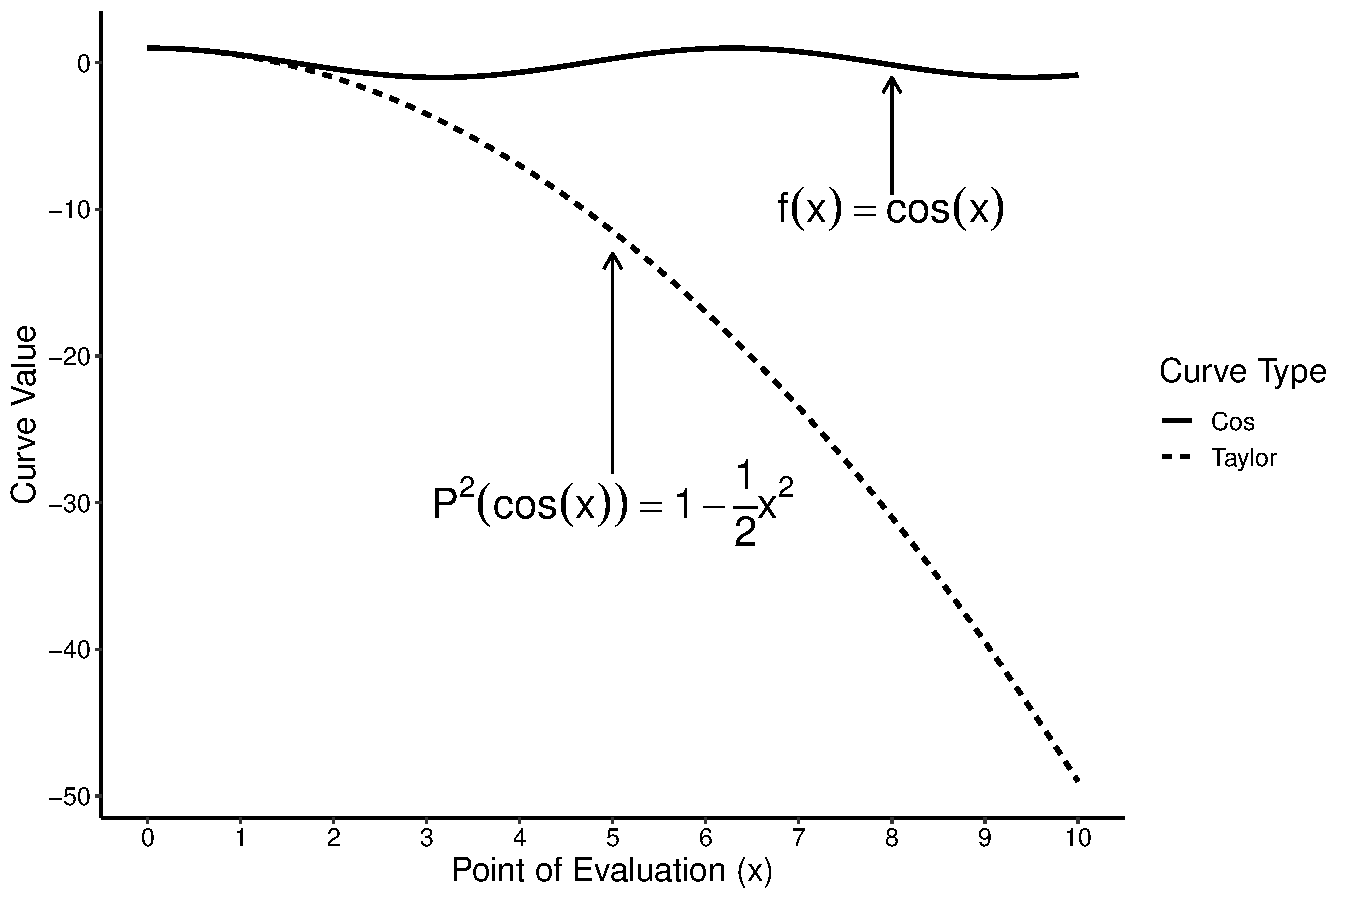
\includegraphics{Figures/taylor_vs_nonlin} \hfill{}
  \caption*{Note. \textup{The second order Taylor series perfectly estimates $\cos(x)$ when the point of evaluation ($x$) equals the point of derivation ($a$; $x = a = 0$), but incurs an increasingly large amount of error as the difference between the point of evaluation and the point of derivation increases. For example, at $x = 10$, $\cos(x) = -0.84$, but the Taylor series outputs a value of -49.50 ($P^2(cos(50)) = 1- \frac{1}{2}10^2 = -49.50$). }}
\end{figure}
\subsubapp{Taylor Series Approximation of the Logistic Function}

Given that a Taylor series provides a linear approximation of a
nonlinear function and the structural equation modelling framework is linear, the structured latent curve modelling approach uses Taylor series approximations to construct linear representations of nonlinear functions (Browne, 1993; Browne \& Du Toit, 1991). In the current simulations, a Taylor series approximation was constructed for the logistic function (Equation \ref{eq:logistic}). Note that, because the logistic function had four parameters (\(\uptheta\),
\(\upalpha\), \(\upbeta\), \(\upgamma\)), derivatives were computed with
respect to each of the parameters. Using a derivative order set to one
(\(n = 1\)), the following Taylor series was constructed for the logistic
function (Equation \ref{eq:logistic-approx}):
\begin{align}
 P^1(L(\Uptheta, t)) = L + \frac{\partial L}{\partial \uptheta}(x_{\uptheta}-a_{\uptheta})^1 + \frac{\partial L}{\partial \upalpha}(x_{\upalpha}-a_{\upalpha})^1 + \frac{\partial L}{\partial \upbeta}(x_{\upbeta}-a_{\upbeta})^1 + \frac{\partial L}{\partial \upgamma_{\upgamma}}(x-a_{\upgamma})^1, 
\label{eq:logistic-approx}
\end{align}
\noindent where \(\mathbf{L(\Uptheta, t)}\) represents the logistic function shown below in
Equation \ref{eq:logistic}:
\begin{align}
  \mathbf{L(\Uptheta, t)} = \uptheta + \frac{\upalpha - \uptheta}{{1 + e^\frac{\upbeta - t}{\upgamma}}} + \upepsilon, 
\label{eq:logistic}
\end{align}
\noindent with \(\Uptheta = [\uptheta, \upalpha, \upbeta, \upgamma]\) and \(\mathbf{L(\Uptheta, t)}\) being a vector of scores at all \(\mathbf{t}\) time points. In the current context, because each parameter of the logistic function had a unique meaning (see section on \protect\hyperlink{data-generation-1}{data generation}), the point of derivation \(a\) differed for each parameter---using the same \(a\) value for each parameter to construct the
Taylor series approximation of the logistic function would have yielded
a practically useless equation. Because the logistic Taylor series
approximation (Equation \ref{eq:logistic-approx}) was deployed in a
statistical model (i.e., the structural equation modelling framework), the derivation values
(\(a_{\uptheta}\), \(a_{\upalpha}\), \(a_{\upbeta}\), \(a_{\upgamma}\)) were set
to the mean values estimated by the analysis for each parameter. Thus, the
derivation values were replaced with the following terms:
\begin{itemize}
\tightlist
\item
  \(a_{\uptheta} = \hat{\uptheta}\)
\item
  \(a_{\upalpha} = \hat{\upalpha}\)
\item
  \(a_{\upbeta} = \hat{\upbeta}\)
\item
  \(a_{\upgamma} = \hat{\upgamma}\)
\end{itemize}
\noindent where that a caret \(\hat{}\) indicates the mean value estimated for a parameter by the analysis. In order to estimate curves for each \(p\) person, the values of
evaluation (\(x_{\uptheta}\), \(x_{\upalpha}\), \(x_{\upbeta}\),
\(x_{\upgamma}\)) corresponded to the parameter values computed for a
given person (\(\uptheta_p\), \(\upalpha_p\), \(\upbeta_p\), \(\upgamma_p\)). Thus, the evaluation values were replaced with the following terms:
\begin{itemize}
\tightlist
\item
  \(x_{\uptheta} = \uptheta_p\)
\item
  \(x_{\upalpha} = \upalpha_p\)
\item
  \(x_{\upbeta} = \upbeta_p\)
\item
  \(x_{\upgamma} = \upgamma_p\)
\end{itemize}
\noindent Substituting the above values for the derivation and evaluation values of \(x\) and \(a\) in the initial logistic Taylor series approximation (Equation \ref{eq:logistic-approx}) yielded the following expression for the logistic Taylor series approximation (Equation \ref{eq:taylor-full}):
\begin{align}
 P^1(L(\Uptheta, t)) = L(\Uptheta, t) + \frac{\partial L}{\partial \uptheta}(\uptheta_i-\hat{\uptheta})^1 + \frac{\partial L}{\partial \upalpha}(\upalpha_i-\hat{\upalpha_i})^1 + \frac{\partial L}{\partial \upbeta}(\upbeta-\hat{\upbeta})^1 + \frac{\partial L}{\partial \upgamma_{\upgamma}}(\upbeta-\hat{\upbeta})^1.
\label{eq:taylor-full}
\end{align}
\noindent Therefore, because the Taylor series was derived using the mean values estimated for each parameter (\(\hat{\uptheta}\), \(\hat{\upalpha}\), \(\hat{\upbeta}\),
\(\hat{\upgamma}\)), it provided a perfect approximation of the estimated
population curve---the evaluation values for each parameter would have
been set to their corresponding mean estimated value. To estimate the curve of any given \(p\) person, the evaluation values could be offset from their corresponding derivation value (i.e., mean estimated value for a parameter) by using the set of parameter values computed for that person (\(\uptheta_p\), \(\upalpha_p\), \(\upbeta_p\), \(\upgamma_p\)). Note that, because Taylor series approximations are only locally accurate, the predicted curves for any given \(p\) person become increasingly inaccurate curves as the difference between the derivation and evaluation values increases (e.g., \(\uptheta_i-\hat{\uptheta}\)).

\subsubapp{Fitting the Logistic Taylor Series Approximation Into the Structual Equation Modelling Framework}

Although the logistic Taylor series approximation provides an accurate
estimation of the logistic function, the function in (Equation
\ref{eq:taylor-full}) is modified in the structured latent curve
modelling approach so that it can more effectively fit into the structural equation modelling framework (Equation \ref{eq:sem-framework}). The partial derivative information is stored in the matrix \(\mathbf{\Uplambda}\) such that

\[ 
\mathbf{\Uplambda} = 
\begin{bmatrix}
\frac{\partial L(\Uptheta, t_1)}{\partial \uptheta} & \frac{\partial L(\Uptheta, t_1)}{\partial \upalpha}  &  \frac{\partial L(\Uptheta, t_1)}{\partial \upbeta} & \frac{\partial L(\Uptheta, t_1)}{\partial \upgamma}   \\ 
\frac{\partial L(\Uptheta, t_2)}{\partial \uptheta}  & \frac{\partial L(\Uptheta, t_2)}{\partial \upalpha} &  \frac{\partial L(\Uptheta, t_2)}{\partial \upbeta} & \frac{\partial L(\Uptheta, t_2)}{\partial \upgamma} & \\ 
\vdots & \vdots & \vdots & \vdots \\ 
\frac{\partial L(\Uptheta, t_n)}{\partial \uptheta} & \frac{\partial L(\Uptheta, t_n)}{\partial \upalpha}  & \frac{\partial L(\Uptheta, t_n)}{\partial \upbeta} & \frac{\partial L(\Uptheta, t_n)}{\partial \upgamma} \\
\end{bmatrix}.
\]

\noindent As in the structural equation modelling framework where each column of
\(\mathbf{\Uplambda}\) specified a basis curve (i.e., a loading of a
growth parameter onto all time points), each column of \(\mathbf{\Uplambda}\) here
in the structured latent curve modelling approach contains the loadings
of a logistic function parameter onto all the \(n\) time points, with the loadings being determined by the partial derivative of logistic function with respect to that parameter. To predict unique curves for each person, each column can be multiplied by a specific weight \(\mathbf{\upiota_p}\) that contains person-specific deviations from each mean estimated parameter value as shown below:

\[ 
\mathbf{\upiota_p} = 
\begin{bmatrix}
\hat{\uptheta} - \uptheta_p   \\ 
\hat{\upalpha} - \upalpha_p   \\ 
\hat{\upbeta} - \upbeta_p \\ 
\hat{\upgamma_i} - \upgamma_p \\
\end{bmatrix},
\]

\noindent where a caret (\(\hat{}\)) indicates the mean value estimated
for a given parameter and a subscript \(p\) indicates a parameter value
computed for a person. With a matrix \(\mathbf{\Uplambda}\) containing
logistic function parameter loadings and a vector \(\mathbf{\upiota_p}\) containing
person-specific weights, the Taylor series of Equation
\ref{eq:taylor-full} that predicted a person's scores over time can be
rewritten to become the following expression of Equation
\ref{eq:slcm-nonsem}:
\begin{align}
 \mathbf{y_p} = \mathbf{L(\Uptheta, t)} + \mathbf{\Uplambda\upiota_p} + \mathbf{\mathcal{E}_p}.
 \label{eq:slcm-nonsem}
\end{align}
\noindent Importantly, because of the logistic function (\(\mathbf{L(\Uptheta, t)}\)) in the
above expression (Equation \ref{eq:slcm-nonsem}), the model no longer
fits into the general structural equation modelling framework (Equation \ref{eq:sem-framework}). To modify Equation \ref{eq:slcm-nonsem} such that it fits into the structural equation modelling framework, the structured latent curve modelling approach recognizes that the logistic function (\(\mathbf{L(\Uptheta, t)}\)) is invariant under a scaling constant and uses this property to rewrite \(\mathbf{L(\Uptheta, t)}\) as a weighted sum of the partial derivative loading matrix (\(\mathbf{\Uplambda}\); Shapiro \& Browne, 1987). Briefly, the
logistic function vector \(\mathbf{L(\Uptheta, t)}\) is invariant under a constant scaling
property because, given some constant scalar value \(k \ge 0\) and a set
of parameter values (\(\Uptheta\)), there exists another set of parameter
values (\(\tilde{\Uptheta}\)) that can produce the same values (see
Equation \ref{eq:icsf} and Example \ref{exm:icsf-ex} below).
\begin{align}
 k\mathbf{L(\Uptheta, t)} = \mathbf{L(\tilde{\Uptheta}, t)}
 \label{eq:icsf}
\end{align}
\begin{example}
\protect\hypertarget{exm:icsf-ex}{}\label{exm:icsf-ex}Invariability under a constant scaling factor of logistic function (Equation \ref{eq:logistic}).

\noindent \textup{Given $t = [0, 1, 2, 3]$, $\Uptheta = [\uptheta = 3.00$, $\upalpha = 3.32$, $\upbeta = 180.00$, $\upgamma = 20.00$], and some constant scaling factor $k = 2.00$, then there exists some set of parameter values $\tilde{\Uptheta}$ that produces the same values as $kL(\Uptheta)$. In the current example, $\tilde{\Uptheta} = [\uptheta = 6.00$, $\upalpha = 6.64$, $\upbeta = 180.00$, $\upgamma = 20.00$].}
\begin{align*}
\mathbf{kL(\Uptheta, t)} &= \mathbf{L(\tilde{\Uptheta}, t)} \nonumber \\ 
2*[3.00, 3.02, 3.30, 3.32] &=  [6.00, 6.04, 6.60, 6.64] \nonumber \\ 
[6.00, 6.04, 6.60, 6.64]  &= [6.00, 6.04, 6.60, 6.64] 1 \nonumber \\ 
\end{align*}
\vspace*{-25mm}

\noindent \hrulefill
\end{example}
\noindent If a function has the property of being invariant under a
scaling factor, then it can also be expressed as the following
matrix-vector product shown in Equation \ref{eq:logistic-matrix-vector}
(Shapiro \& Browne, 1987):
\begin{align}
 \mathbf{L(\Uptheta, t)} = \mathbf{\Lambda\uptau},
\label{eq:logistic-matrix-vector}
\end{align}
\noindent where \(\mathbf{\Uplambda}\) contains the partial derivative loadings\footnote{This is also known as a Jacobian matrix.} and
\(\mathbf{\uptau}\) is a vector whose values are otbained by pre-multiplying the output of the logistic function (\(\mathbf{L(\Uptheta, t)}\)) by the inverse of the partial derivative loading matrix \({\Lambda\uptau}^{-1}\). Solving for \(\mathbf{\uptau}\) yields a vector whose contents contain the mean values estimated for parameters that enter the logistic function in a linear way and
zeroes for parameters that enter the function in a nonlinear way (i.e.,
parameters that exist within their own partial derivative). Hence, \(\mathbf{\uptau}\) is often called a mean vector (Blozis, 2004; K. J. Preacher \& Hancock, 2015). In the current example, \(\uptheta\) and \(\upalpha\) enter the logistic function
in a linear way and \(\upbeta\) and \(\upgamma\) enter the logistic function
in a nonlinear way and so the first two entries of \(\mathbf{\uptau}\)
contain the values estimated for \(\uptheta\) and \(\upalpha\) (i.e.,
\(\hat{\uptheta}\) and \(\hat{\upalpha}\)) and the last two entries contain zeroes. Example \ref{exm:tau-vector} below shows that the first two
values of \(\mathbf{\uptau}\) are indeed the values estimated for
\(\uptheta\) and \(\upalpha\) and the last two values are zero.
\begin{example}
\protect\hypertarget{exm:tau-vector}{}\label{exm:tau-vector}Computation of mean vector \(\mathbf{\uptau}\).

\noindent \textup{Given the parameter estimates of $\hat{\uptheta} = 3.00$, $\hat{\upalpha} = 3.32$, $\hat{\upbeta} = 180.00$, and $\hat{\upgamma} = 20.00$ and $\mathbf{t}$ = [0, 1, 2, 3], $\mathbf{\uptau}$ = [3.00, 3.32, 0, 0], then }
\begin{align*}
\mathbf{L(\Uptheta, t)} &= \mathbf{\Lambda\uptau} \\ 
[3.00, 3.02, 3.30, 3.32] &= \begin{bmatrix}
1.00 & 0.00 & 0.00  & 0.00 \\ 
0.95  & 0.05 & -0.00 & 0.00 \\ 
0.05 & 0.95 & -0.00 & -0.00 \\ 
0.00 & 1.00  & 0.00 & 0.00 \\
\end{bmatrix} \mathbf{\uptau} \\ 
\begin{bmatrix}
1.00 & 0.00 & 0.00  & 0.00 \\ 
0.95  & 0.05 & -0.00 & 0.00 \\ 
0.05 & 0.95 & -0.00 & -0.00 \\ 
0.00 & 1.00  & 0.00 & 0.00 \\
\end{bmatrix}^{-1}
\begin{bmatrix} 
3.00 \\ 3.02 \\ 3.30 \\ 3.32
\end{bmatrix} &=  \mathbf{\Lambda\uptau} \\ 
 \mathbf{\uptau} &= [3.00, 3.32, 0, 0]\\
\end{align*}
\vspace*{-25mm}

\noindent \hrulefill
\end{example}
\noindent With \(\mathbf{L(\Uptheta, t)} = \mathbf{\Uplambda\uptau}\), Equation \ref{eq:slcm-nonsem} can be rewritten in a linear equation as shown below in Equation \ref{eq:taylor-linear}:
\begin{align}
 \mathbf{y_p} = \mathbf{\Uplambda\uptau} + \mathbf{\Uplambda\upiota_p} + \mathbf{\mathcal{E}_p}.
 \label{eq:taylor-linear}
 \end{align}
\noindent The mean vector \(\mathbf{\uptau}\) and vector of
person-specific deviations \(\mathbf{\upiota_p}\) can be combined into a
new vector \(\mathbf{s_p}\) that represents the person-specific weights
applied to the basis curves in \(\mathbf{\Uplambda}\) such that

\[  
\mathbf{s_p} = \mathbf{\uptau + \upiota_p} =
\begin{bmatrix} 
\hat{\uptheta} + \hat{\uptheta} - \uptheta_p \\ 
\hat{\upalpha} + \hat{\upalpha} - \upalpha_p \\ 
0 + \hat{\upbeta} - \upbeta_p \\ 
0 + \hat{\upgamma} - \upgamma_p \\ 
\end{bmatrix}
\]

\noindent and
\begin{align}
\mathbf{y_p} = \mathbf{\Uplambda s_p} + \mathbf{\mathcal{E}_p}. 
\label{eq:taylor-final}
\end{align}
\noindent Because the expected value of the person-specific weights
(\(\mathbf{s_p}\)) is the mean vector (\(\mathbf{\uptau}\);
\(\mathbb{E}[{\mathbf{s_p}}] = \mathbf{\uptau}\), the expected set
of scores predicted across all people (\(\mathbb{E}[{\mathbf{y_p}}]\)) gives back the original expression for the logistic function matrix-vector product in Equation
\ref{eq:logistic-matrix-vector} as shown below in Equation \ref{eq:expected-value}:
\begin{align}
 \mathbb{E}[{\mathbf{y_p}}] = \mathbf{\Uplambda\uptau} = \mathbf{L(\Uptheta, t)}. 
\label{eq:expected-value}
\end{align}
\noindent Therefore, the structured latent curve modelling approach
successfully reproduces the output of the nonlinear logistic function
(Equation \ref{eq:logistic}) with the linear function of Equation
\ref{eq:taylor-final}. Note that that no error term exists in Equation \ref{eq:expected-value} because the expected value of the error
values is zero (\(\mathbb{E}[{\mathbf{\mathcal{E}_p}}] = 0\)).

\subsubapp{Estimating Parameters in the Structured Latent Curve Modelling Approach}

To estimate parameter values, the full-information maximum
likelihood shown in Equation \ref{eq:fiml-person} was computed for each
person (i.e., likelihood of observing a \(p\) person's data given the
estimated parameter values):
\begin{align}
\mathcal{L}_p = k_p \ln(2\pi) + \ln(|\mathbf{\Sigma_p}| + (\mathbf{y_p} - \mathbf{\upmu_p})^\top \mathbf{\Sigma_p}^{-1}(\mathbf{y_p} - \mathbf{\upmu_p}),
\label{eq:fiml-person}
\end{align}
\noindent where \(k_p\) is the number of non-missing values for a given
\(p\) person, \(\mathbf{\Sigma_p}\) is the model-implied covariance matrix
with rows and columns filtered at time points where person \(p\) has
missing data, \(\mathbf{y_p}\) is a vector containing the data points that
were collected for a \(p\) person (i.e., filtered data), and
\(\mathbf{\upmu_p}\) is the model-implied mean vector that is filtered at
time points where person \(p\) has missing data. Note that, because all
simulations assumed complete data across all times points, no filtering
procedures were executed (for a review of the filtering procedure, see Boker et al., 2020, Chapter 5). Thus, computing the above full-information
maximum likelihood in Equation \ref{eq:fiml-person} was equivalent to
computing the below likelihood function in Equation
\ref{eq:ml-estimation}:
\begin{align}
\mathcal{L}_p = k_p \ln(2\pi) + \ln(|\mathbf{\Sigma}| + (\mathbf{y_p} - \mathbf{\upmu})^\top \mathbf{\Sigma}^{-1}(\mathbf{y_p} - \mathbf{\upmu}),  
\label{eq:ml-estimation}
\end{align}
\noindent where \(\mathbf{\Sigma}\) is the model-implied covariance matrix,
\(\mathbf{y_p}\) contains the data collected from a \(p\) person, and
\(\mathbf{\upmu}\) is the model-implied mean vector. The model-implied
covariance matrix \(\mathbf{\Sigma}\) is computed using Equation
\ref{eq:covariance} below:
\begin{align}
\mathbf{\Sigma} = \mathbf{\Uplambda\Uppsi\Uplambda} + \mathbf{\Upomega}_{\mathcal{E}},   
\label{eq:covariance}
\end{align}
\noindent where \(\mathbf{\Uppsi}\) is the random-effect covariance matrix
and \(\mathbf{\Upomega}_{\mathcal{E}}\) contains the error variances at
each time point. The mean vector \(\mathbf{\upmu}\) was computed using
Equation \ref{eq:mean-structure} shown below:
\begin{align}
\mathbf{\upmu} = \mathbf{\Uplambda\uptau}. 
\label{eq:mean-structure}
\end{align}
\noindent Parameter estimation was conducted by finding values for the model-implied
covariance matrix \(\mathbf{\Sigma}\) and the model-implied mean vector
\(\mathbf{\upmu}\) that maximized the sum of log-likelihoods across all \(P\) people
(see Equation \ref{eq:max-ll} below):
\begin{align}
\mathcal{L} = \underset{\mathbf{\Sigma},\mathbf{\upmu} }{\argmax} \sum^P_{p = 1} \mathcal{L}_p.
\label{eq:max-ll}
\end{align}
\noindent In OpenMx, the above problem was solved using the sequential
least squares quadratic program (for a review, see Kraft, 1994).

\app{Procedure for Generating Measurement Schedules Measurement SchedulesMeasurement Schedules}

Given that no procedure existed (to my knowledge) for creating
measurement schedules, I devised a method for generating measurement
schedules for the four spacing conditions (equal, time-interval
increasing, time-interval decreasing, and middle-and-extreme spacing).
For each measurement spacing conditions across all measurement number
levels, a two-step procedure was employed to generate measurement
schedules in Experiments 2--3. At a broad level, the first step involved
computing setup variables and the second step computed the interval
lengths.

\secapp{Procedure for Constructing Measurement Schedules With Equal Spacing}

Figure @ref\{fig:equal\_spacing\_diagram\} shows how the two-step procedure
was implemented to construct a measurement schedule with equal spacing
and five measurements. In the first step, the number of intervals (\(NI\))
was computed by subtracting one from the number of measurements (\(NM\)),
giving five measurements (\(NM = 5\)) and four intervals (\(NI = 4\)). In
the second step, interval lengths were calculated by dividing the length
of the measurement period (\(MP\)) by the number of intervals (\(NI\)),
yielding an interval length of 90 days
(\(\frac{MP}{NI} = \frac{360}{4} = 90\)).
\begin{apaFigure}
[landscape]
[samepage]
{Procedure for Generating Equal Spacing Schedules With Equal Spacing}
{equal_spacing_diagram}
{0.75}
{Figures/equal_spacing_diagram}
{}
\end{apaFigure}
\secapp{Procedure for Constructing Measurement Schedules With Time-Interval Increasing Spacing}

Figure @ref\{fig:time\_inc\_diagram\} shows how the two-step procedure was
used to calculate the interval lengths for measurement schedules defined
by time-interval increasing spacing with five measurements. In the first
step, the number of intervals was determined by subtracting one from the
number of measurements, yielding a value of four for the number of
intervals (\(NI = NM - 1 = 5 - 1 = 4\)). Importantly, the length of each
interval increased by a constant value \(c\) over time as shown below in
Equation \ref{eq:time-inc-length}:
\begin{align}
\text{Interval length} = x + \#IN(c)
\label{eq:time-inc-length}
\end{align}
\noindent where \(\#IN\) represents the interval number in increasing
order such that
\(\#IN \in \{0, ..., \text{number of intervals (NI)} - 1\}\). In the
second step, the constant value by which interval lengths increased
(\(c\)) was computed by first subtracting the smallest interval length
from each interval (i.e., \(x = 36\) days) from the measurement period
(\(MP\)), yielding 216 remaining days
(\(N_{remain} = MP - NIx = 360 - 4(36) = 216\)). The number of remaining
days then had to be divided across the constant interval lengths.
Because each interval increased by some constant value (\(c\) after each
measurement point, the total number of constant-value interval lengths
was obtained by computing the following sum in Equation
\ref{eq:time-sum-constants}:
\begin{align}
\text{Number constant intervals} = \sum^{\#IN}_{i = 0} i.
\label{eq:time-sum-constants}
\end{align}
\noindent With \(\#IN = 3\), the number of constant intervals was 6, and
so the constant value was obtained by using Equation
\ref{eq:constant-length} below:
\begin{align}
\text{Number constant intervals} = \frac{N_{remain}}{\sum^{\#IN}_{i = 0} i},
\label{eq:constant-length}
\end{align}
\noindent giving a length of 36 days for the constant value
(\(c = \frac{216}{6} = 36\) days). Having computed the value for \(c\), the
following interval lengths were obtained:
\begin{itemize}
\tightlist
\item
  \(i_{1} = x + \#IN(c) = 36 + 0(36)\) = 36 days
\item
  \(i_{2} = x + \#IN(c) = 36 + 1(36)\) = 72 days
\item
  \(i_{3} = x + \#IN(c) = 36 + 2(36)\) = 108 days
\item
  \(i_{4} = x + \#IN(c) = 36 + 3(36)\) = 144 days
\end{itemize}
\begin{apaFigure}
[landscape]
[samepage]
{Procedure for Generating Equal Spacing Schedules With Time-Interval Increasing Spacing}
{time_inc_diagram}
{0.75}
{Figures/time_inc_diagram}
{}
\end{apaFigure}
\secapp{Procedure for Constructing Measurement Schedules With Time-Interval Decreasing Spacing}

Figure @ref\{fig:time\_dec\_diagram\} shows how the two-step procedure was
used to calculate the interval lengths for measurement schedules defined
by time-interval decreasing spacing with five measurements. In the first
step, the number of intervals was determined by subtracting one from the
number of measurements, yielding a value of four for the number of
intervals (\(NI = NM - 1 = 5 - 1 = 4\)). Importantly, the length of each
interval decreased by a constant value \(c\) over time as shown below in
Equation \ref{eq:time-dec-length}:
\begin{align}
\text{Interval length} = x + \#INT(c)
\label{eq:time-dec-length}
\end{align}
\noindent where \(\#IN\) represents the interval number in decreasing
order such that
\(\#IN \in \{\text{number of intervals (NI)} - 1, ... , 0\}\). In the
second step, the constant value by which interval lengths decreased
(\(c\)) was computed by first subtracting the smallest interval length
from each interval (i.e., \(x = 36\) days) from the measurement period
(\(MP\)), yielding 216 remaining days
(\(N_{remain} = MP - NIx = 360 - 4(36) = 216\)). The number of remaining
days then had to be divided across the constant interval lengths.
Because each interval decreased by some constant value (\(c\) after each
measurement point, the total number of constant-value interval lengths
was obtained by computing the following sum in Equation
\ref{eq:dec-sum-constants}:
\begin{align}
\text{Number constant intervals} = \sum_{\#IN}^{i = 0} i.
\label{eq:dec-sum-constants}
\end{align}
\noindent With \(\#IN = 3\), the number of constant intervals was 6, and
so the constant value was obtained by using Equation
\ref{eq:constant-length-2} below:
\begin{align}
\text{Number constant intervals} = \frac{N_{remain}}{\sum^{\#IN}_{i = 0} i},
\label{eq:constant-length-2}
\end{align}
\noindent giving a length of 36 days for the constant value
(\(c = \frac{216}{6} = 36\) days). Having computed the value for \(c\), the
following interval lengths were obtained:
\begin{itemize}
\tightlist
\item
  \(i_{1} = x + \#IN(c) = 36 + 3(36)\) = 144 days
\item
  \(i_{4} = x + \#IN(c) = 36 + 0(36)\) = 36 days
\item
  \(i_{3} = x + \#IN(c) = 36 + 1(36)\) = 72 days
\item
  \(i_{2} = x + \#IN(c) = 36 + 2(36)\) = 108 days
\end{itemize}
\begin{apaFigure}
[landscape]
[samepage]
{Procedure for Generating Equal Spacing Schedules With Time-Interval Decreasing Spacing}
{time_dec_diagram}
{0.75}
{Figures/time_dec_diagram}
{}
\end{apaFigure}
\secapp{Procedure for Constructing Measurement Schedules With Middle-and-Extreme Spacing}

Figure @ref\{fig:mid\_ext\_diagram\} shows how the two-step procedure was
used to calculate the interval lengths for measurement schedules defined
by middle-and-extreme spacing with five measurements. In the first step,
the number of intervals was determined by subtracting one from the
number of measurements, yielding a value of four for the number of
intervals (\(NI = NM - 1 = 5 - 1 = 4\))\ldots{}

\app{Convergence Success Rates}
\begin{ThreePartTable}
\begin{TableNotes}
\item \textit{Note. }Cells shaded in gray indicate conditions where less than 90\% of models converged.
\end{TableNotes}
\begin{longtable}[l]{>{\raggedright\arraybackslash}p{3cm}>{\raggedright\arraybackslash}p{3cm}>{\centering\arraybackslash}p{1cm}>{\centering\arraybackslash}p{1cm}>{\centering\arraybackslash}p{1cm}>{}p{1cm}>{}p{1cm}>{}p{1cm}>{}p{1cm}>{}p{1cm}>{}p{1cm}>{}p{1cm}>{}p{1cm}>{}p{1cm}>{}p{1cm}>{}p{1cm}}
\caption{\label{tab:conv-exp-1}Convergence Success in Experiment 1}\\
\toprule
\multicolumn{1}{c}{} & \multicolumn{1}{c}{} & \multicolumn{3}{c}{Days to halfway elevation} \\
\cmidrule(l{3pt}r{3pt}){3-5}
Measurement Spacing & Number of Measurements & 80 & 180 & 280\\
\midrule
 & 5 & \cellcolor[HTML]{ffffff}{1.00} & \cellcolor[HTML]{ffffff}{0.98} & \cellcolor[HTML]{ffffff}{0.95}\\
\nopagebreak
 & 7 & \cellcolor[HTML]{ffffff}{1.00} & \cellcolor[HTML]{ffffff}{1.00} & \cellcolor[HTML]{ffffff}{0.99}\\
\nopagebreak
 & 9 & \cellcolor[HTML]{ffffff}{1.00} & \cellcolor[HTML]{ffffff}{1.00} & \cellcolor[HTML]{ffffff}{1.00}\\
\nopagebreak
\multirow{-4}{3cm}{\raggedright\arraybackslash Equal} & 11 & \cellcolor[HTML]{ffffff}{1.00} & \cellcolor[HTML]{ffffff}{1.00} & \cellcolor[HTML]{ffffff}{1.00}\\
\cmidrule{1-5}\pagebreak[0]
 & 5 & \cellcolor[HTML]{ffffff}{1.00} & \cellcolor[HTML]{ffffff}{1.00} & \cellcolor[HTML]{ffffff}{1.00}\\
\nopagebreak
 & 7 & \cellcolor[HTML]{ffffff}{1.00} & \cellcolor[HTML]{ffffff}{1.00} & \cellcolor[HTML]{ffffff}{1.00}\\
\nopagebreak
 & 9 & \cellcolor[HTML]{ffffff}{1.00} & \cellcolor[HTML]{ffffff}{1.00} & \cellcolor[HTML]{ffffff}{1.00}\\
\nopagebreak
\multirow{-4}{3cm}{\raggedright\arraybackslash Time-interval increasing} & 11 & \cellcolor[HTML]{ffffff}{1.00} & \cellcolor[HTML]{ffffff}{1.00} & \cellcolor[HTML]{ffffff}{1.00}\\
\cmidrule{1-5}\pagebreak[0]
 & 5 & \cellcolor[HTML]{ffffff}{1.00} & \cellcolor[HTML]{ffffff}{0.96} & \cellcolor[HTML]{eeeeee}{0.82}\\
\nopagebreak
 & 7 & \cellcolor[HTML]{ffffff}{1.00} & \cellcolor[HTML]{ffffff}{0.99} & \cellcolor[HTML]{ffffff}{0.98}\\
\nopagebreak
 & 9 & \cellcolor[HTML]{ffffff}{1.00} & \cellcolor[HTML]{ffffff}{1.00} & \cellcolor[HTML]{ffffff}{1.00}\\
\nopagebreak
\multirow{-4}{3cm}{\raggedright\arraybackslash Time-interval decreasing} & 11 & \cellcolor[HTML]{ffffff}{1.00} & \cellcolor[HTML]{ffffff}{1.00} & \cellcolor[HTML]{ffffff}{1.00}\\
\cmidrule{1-5}\pagebreak[0]
 & 5 & \cellcolor[HTML]{ffffff}{1.00} & \cellcolor[HTML]{ffffff}{0.96} & \cellcolor[HTML]{eeeeee}{0.86}\\
\nopagebreak
 & 7 & \cellcolor[HTML]{ffffff}{1.00} & \cellcolor[HTML]{ffffff}{1.00} & \cellcolor[HTML]{ffffff}{1.00}\\
\nopagebreak
 & 9 & \cellcolor[HTML]{ffffff}{1.00} & \cellcolor[HTML]{ffffff}{1.00} & \cellcolor[HTML]{ffffff}{1.00}\\
\nopagebreak
\multirow{-4}{3cm}{\raggedright\arraybackslash Middle-and-extreme} & 11 & \cellcolor[HTML]{ffffff}{1.00} & \cellcolor[HTML]{ffffff}{1.00} & \cellcolor[HTML]{ffffff}{1.00}\\
\bottomrule
\insertTableNotes
\end{longtable}
\end{ThreePartTable}
\begin{ThreePartTable}
\begin{TableNotes}
\item \textit{Note. }Cells shaded in gray indicate conditions where less than 90\% of models converged.
\end{TableNotes}
\begin{longtable}[l]{>{\raggedright\arraybackslash}p{3cm}>{\raggedright\arraybackslash}p{3cm}>{\centering\arraybackslash}p{1cm}>{\centering\arraybackslash}p{1cm}>{\centering\arraybackslash}p{1cm}>{\centering\arraybackslash}p{1cm}>{\centering\arraybackslash}p{1cm}>{\centering\arraybackslash}p{1cm}>{}p{1cm}>{}p{1cm}>{}p{1cm}>{}p{1cm}>{}p{1cm}>{}p{1cm}>{}p{1cm}>{}p{1cm}}
\caption{\label{tab:conv-exp-2}Convergence Success in Experiment 2}\\
\toprule
\multicolumn{1}{c}{} & \multicolumn{1}{c}{} & \multicolumn{6}{c}{Sample size (\textit{N})} \\
\cmidrule(l{3pt}r{3pt}){3-8}
Measurement Spacing & Number of Measurements & 30 & 50 & 100 & 200 & 500 & 1000\\
\midrule
 & 5 & \cellcolor[HTML]{ffffff}{1.00} & \cellcolor[HTML]{ffffff}{1.00} & \cellcolor[HTML]{ffffff}{0.99} & \cellcolor[HTML]{ffffff}{0.98} & \cellcolor[HTML]{ffffff}{0.95} & \cellcolor[HTML]{ffffff}{0.92}\\
\nopagebreak
 & 7 & \cellcolor[HTML]{ffffff}{1.00} & \cellcolor[HTML]{ffffff}{1.00} & \cellcolor[HTML]{ffffff}{1.00} & \cellcolor[HTML]{ffffff}{1.00} & \cellcolor[HTML]{ffffff}{0.99} & \cellcolor[HTML]{ffffff}{0.98}\\
\nopagebreak
 & 9 & \cellcolor[HTML]{ffffff}{1.00} & \cellcolor[HTML]{ffffff}{1.00} & \cellcolor[HTML]{ffffff}{1.00} & \cellcolor[HTML]{ffffff}{1.00} & \cellcolor[HTML]{ffffff}{1.00} & \cellcolor[HTML]{ffffff}{1.00}\\
\nopagebreak
\multirow{-4}{3cm}{\raggedright\arraybackslash Equal} & 11 & \cellcolor[HTML]{ffffff}{1.00} & \cellcolor[HTML]{ffffff}{1.00} & \cellcolor[HTML]{ffffff}{1.00} & \cellcolor[HTML]{ffffff}{1.00} & \cellcolor[HTML]{ffffff}{1.00} & \cellcolor[HTML]{ffffff}{1.00}\\
\cmidrule{1-8}\pagebreak[0]
 & 5 & \cellcolor[HTML]{ffffff}{1.00} & \cellcolor[HTML]{ffffff}{1.00} & \cellcolor[HTML]{ffffff}{1.00} & \cellcolor[HTML]{ffffff}{1.00} & \cellcolor[HTML]{ffffff}{1.00} & \cellcolor[HTML]{ffffff}{1.00}\\
\nopagebreak
 & 7 & \cellcolor[HTML]{ffffff}{1.00} & \cellcolor[HTML]{ffffff}{1.00} & \cellcolor[HTML]{ffffff}{1.00} & \cellcolor[HTML]{ffffff}{1.00} & \cellcolor[HTML]{ffffff}{1.00} & \cellcolor[HTML]{ffffff}{1.00}\\
\nopagebreak
 & 9 & \cellcolor[HTML]{ffffff}{1.00} & \cellcolor[HTML]{ffffff}{1.00} & \cellcolor[HTML]{ffffff}{1.00} & \cellcolor[HTML]{ffffff}{1.00} & \cellcolor[HTML]{ffffff}{1.00} & \cellcolor[HTML]{ffffff}{1.00}\\
\nopagebreak
\multirow{-4}{3cm}{\raggedright\arraybackslash Time-interval increasing} & 11 & \cellcolor[HTML]{ffffff}{1.00} & \cellcolor[HTML]{ffffff}{1.00} & \cellcolor[HTML]{ffffff}{1.00} & \cellcolor[HTML]{ffffff}{1.00} & \cellcolor[HTML]{ffffff}{1.00} & \cellcolor[HTML]{ffffff}{1.00}\\
\cmidrule{1-8}\pagebreak[0]
 & 5 & \cellcolor[HTML]{ffffff}{1.00} & \cellcolor[HTML]{ffffff}{0.99} & \cellcolor[HTML]{ffffff}{0.98} & \cellcolor[HTML]{ffffff}{0.95} & \cellcolor[HTML]{ffffff}{0.93} & \cellcolor[HTML]{eeeeee}{0.88}\\
\nopagebreak
 & 7 & \cellcolor[HTML]{ffffff}{1.00} & \cellcolor[HTML]{ffffff}{1.00} & \cellcolor[HTML]{ffffff}{0.99} & \cellcolor[HTML]{ffffff}{0.99} & \cellcolor[HTML]{ffffff}{0.98} & \cellcolor[HTML]{ffffff}{0.95}\\
\nopagebreak
 & 9 & \cellcolor[HTML]{ffffff}{1.00} & \cellcolor[HTML]{ffffff}{1.00} & \cellcolor[HTML]{ffffff}{1.00} & \cellcolor[HTML]{ffffff}{1.00} & \cellcolor[HTML]{ffffff}{1.00} & \cellcolor[HTML]{ffffff}{0.99}\\
\nopagebreak
\multirow{-4}{3cm}{\raggedright\arraybackslash Time-interval decreasing} & 11 & \cellcolor[HTML]{ffffff}{1.00} & \cellcolor[HTML]{ffffff}{1.00} & \cellcolor[HTML]{ffffff}{1.00} & \cellcolor[HTML]{ffffff}{1.00} & \cellcolor[HTML]{ffffff}{1.00} & \cellcolor[HTML]{ffffff}{1.00}\\
\cmidrule{1-8}\pagebreak[0]
 & 5 & \cellcolor[HTML]{ffffff}{1.00} & \cellcolor[HTML]{ffffff}{0.99} & \cellcolor[HTML]{ffffff}{0.98} & \cellcolor[HTML]{ffffff}{0.96} & \cellcolor[HTML]{eeeeee}{0.90} & \cellcolor[HTML]{eeeeee}{0.81}\\
\nopagebreak
 & 7 & \cellcolor[HTML]{ffffff}{1.00} & \cellcolor[HTML]{ffffff}{1.00} & \cellcolor[HTML]{ffffff}{1.00} & \cellcolor[HTML]{ffffff}{1.00} & \cellcolor[HTML]{ffffff}{1.00} & \cellcolor[HTML]{ffffff}{1.00}\\
\nopagebreak
 & 9 & \cellcolor[HTML]{ffffff}{1.00} & \cellcolor[HTML]{ffffff}{1.00} & \cellcolor[HTML]{ffffff}{1.00} & \cellcolor[HTML]{ffffff}{1.00} & \cellcolor[HTML]{ffffff}{1.00} & \cellcolor[HTML]{ffffff}{1.00}\\
\nopagebreak
\multirow{-4}{3cm}{\raggedright\arraybackslash Middle-and-extreme} & 11 & \cellcolor[HTML]{ffffff}{1.00} & \cellcolor[HTML]{ffffff}{1.00} & \cellcolor[HTML]{ffffff}{1.00} & \cellcolor[HTML]{ffffff}{1.00} & \cellcolor[HTML]{ffffff}{1.00} & \cellcolor[HTML]{ffffff}{1.00}\\
\bottomrule
\insertTableNotes
\end{longtable}
\end{ThreePartTable}
\begin{ThreePartTable}
\begin{TableNotes}
\item \textit{Note. }Cells shaded in gray indicate conditions where less than 90\% of models converged.
\end{TableNotes}
\begin{longtable}[l]{>{\raggedright\arraybackslash}p{3cm}>{\raggedright\arraybackslash}p{3cm}>{\centering\arraybackslash}p{1cm}>{\centering\arraybackslash}p{1cm}>{\centering\arraybackslash}p{1cm}>{\centering\arraybackslash}p{1cm}>{\centering\arraybackslash}p{1cm}>{\centering\arraybackslash}p{1cm}>{}p{1cm}>{}p{1cm}>{}p{1cm}>{}p{1cm}}
\caption{\label{tab:conv-exp-3}Convergence Success in Experiment 3}\\
\toprule
\multicolumn{1}{c}{} & \multicolumn{1}{c}{} & \multicolumn{6}{c}{Sample size (\textit{N})} \\
\cmidrule(l{3pt}r{3pt}){3-8}
Time Structuredness & Number of Measurements & 30 & 50 & 100 & 200 & 500 & 1000\\
\midrule
 & 5 & \cellcolor[HTML]{ffffff}{1.00} & \cellcolor[HTML]{ffffff}{0.99} & \cellcolor[HTML]{ffffff}{0.99} & \cellcolor[HTML]{ffffff}{0.98} & \cellcolor[HTML]{ffffff}{0.96} & \cellcolor[HTML]{eeeeee}{0.90}\\
\nopagebreak
 & 7 & \cellcolor[HTML]{ffffff}{1.00} & \cellcolor[HTML]{ffffff}{1.00} & \cellcolor[HTML]{ffffff}{1.00} & \cellcolor[HTML]{ffffff}{1.00} & \cellcolor[HTML]{ffffff}{0.99} & \cellcolor[HTML]{ffffff}{0.98}\\
\nopagebreak
 & 9 & \cellcolor[HTML]{ffffff}{1.00} & \cellcolor[HTML]{ffffff}{1.00} & \cellcolor[HTML]{ffffff}{1.00} & \cellcolor[HTML]{ffffff}{1.00} & \cellcolor[HTML]{ffffff}{1.00} & \cellcolor[HTML]{ffffff}{1.00}\\
\nopagebreak
\multirow{-4}{3cm}{\raggedright\arraybackslash Time structured} & 11 & \cellcolor[HTML]{ffffff}{1.00} & \cellcolor[HTML]{ffffff}{1.00} & \cellcolor[HTML]{ffffff}{1.00} & \cellcolor[HTML]{ffffff}{1.00} & \cellcolor[HTML]{ffffff}{1.00} & \cellcolor[HTML]{ffffff}{1.00}\\
\cmidrule{1-8}\pagebreak[0]
 & 5 & \cellcolor[HTML]{ffffff}{1.00} & \cellcolor[HTML]{ffffff}{1.00} & \cellcolor[HTML]{ffffff}{0.98} & \cellcolor[HTML]{ffffff}{0.99} & \cellcolor[HTML]{ffffff}{0.96} & \cellcolor[HTML]{ffffff}{0.90}\\
\nopagebreak
 & 7 & \cellcolor[HTML]{ffffff}{1.00} & \cellcolor[HTML]{ffffff}{1.00} & \cellcolor[HTML]{ffffff}{1.00} & \cellcolor[HTML]{ffffff}{0.99} & \cellcolor[HTML]{ffffff}{0.98} & \cellcolor[HTML]{ffffff}{0.99}\\
\nopagebreak
 & 9 & \cellcolor[HTML]{ffffff}{1.00} & \cellcolor[HTML]{ffffff}{1.00} & \cellcolor[HTML]{ffffff}{1.00} & \cellcolor[HTML]{ffffff}{1.00} & \cellcolor[HTML]{ffffff}{1.00} & \cellcolor[HTML]{ffffff}{1.00}\\
\nopagebreak
\multirow{-4}{3cm}{\raggedright\arraybackslash Time unstructured (fast response)} & 11 & \cellcolor[HTML]{ffffff}{1.00} & \cellcolor[HTML]{ffffff}{1.00} & \cellcolor[HTML]{ffffff}{1.00} & \cellcolor[HTML]{ffffff}{1.00} & \cellcolor[HTML]{ffffff}{1.00} & \cellcolor[HTML]{ffffff}{1.00}\\
\cmidrule{1-8}\pagebreak[0]
 & 5 & \cellcolor[HTML]{ffffff}{1.00} & \cellcolor[HTML]{ffffff}{1.00} & \cellcolor[HTML]{ffffff}{0.99} & \cellcolor[HTML]{ffffff}{1.00} & \cellcolor[HTML]{ffffff}{0.95} & \cellcolor[HTML]{ffffff}{0.92}\\
\nopagebreak
 & 7 & \cellcolor[HTML]{ffffff}{1.00} & \cellcolor[HTML]{ffffff}{1.00} & \cellcolor[HTML]{ffffff}{1.00} & \cellcolor[HTML]{ffffff}{0.99} & \cellcolor[HTML]{ffffff}{0.99} & \cellcolor[HTML]{ffffff}{0.98}\\
\nopagebreak
 & 9 & \cellcolor[HTML]{ffffff}{1.00} & \cellcolor[HTML]{ffffff}{1.00} & \cellcolor[HTML]{ffffff}{1.00} & \cellcolor[HTML]{ffffff}{1.00} & \cellcolor[HTML]{ffffff}{1.00} & \cellcolor[HTML]{ffffff}{1.00}\\
\nopagebreak
\multirow{-4}{3cm}{\raggedright\arraybackslash Time unstructured (slow response)} & 11 & \cellcolor[HTML]{ffffff}{1.00} & \cellcolor[HTML]{ffffff}{1.00} & \cellcolor[HTML]{ffffff}{1.00} & \cellcolor[HTML]{ffffff}{1.00} & \cellcolor[HTML]{ffffff}{1.00} & \cellcolor[HTML]{ffffff}{1.00}\\
\bottomrule
\insertTableNotes
\end{longtable}
\end{ThreePartTable}
\app{Complete Versions of Parameter Estimation Plots (Day- and Likert-Unit Parameters)}

\secapp{Experiment 1}
\subapp{Equal Spacing}
\begin{apaFigure}
[portrait]
[samepage]
[0cm]
{Parameter Estimation Plots for Day- and Likert-Unit Parameters With Equal Spacing in Experiment 1}
{exp1_plot_equal_app}
{0.16}
{Figures/exp1_plot_days_equal spacing}
{}
\end{apaFigure}
\addtocounter{figure}{-1}
\begin{apaFigure}
[portrait]
[samepage]
[0cm]
{Parameter Estimation Plots for Day- and Likert-Unit Parameters With Equal Spacing in Experiment 1 (continued)}
{exp1_plot_equal_app}
{0.16}
{Figures/exp1_plot_likert_equal spacing}
{Panels A--B:  Parameter estimation plots for the fixed- and random-effect days-to-halfway elevation parameters, respectively ($\upbeta_{fixed}$ and $\upbeta_{random}$). Panels C--D: Parameter estimation plots for the fixed- and random-effect triquarter-halfway elevation parameters, respectively ($\upgamma_{fixed}$ and $\upgamma_{random}$). Panels E--F: Parameter estimation plots for the fixed- and random-effect baseline parameters, respectively ($\uptheta_{fixed}$ and $\uptheta_{random}$). Panels G--H: Parameter estimation plots for the fixed- and random-effect maximal elevation parameters, respectively ($\upalpha_{fixed}$ and $\upalpha_{random}$). Blue horizontal lines in each panel represent the population value for each parameter. Population values for each day-unit parameter are as follows: $\upbeta_{fixed} \in$ {80, 180, 280}, $\upbeta_{random}$ = 10.00, $\upgamma_{fixed}$ = 20.00, $\upgamma_{random}$ = 4.00, $\uptheta_{fixed}$ = 3.00, $\uptheta_{random}$ = 0.05, $\upalpha_{fixed}$ = 3.32, $\upalpha_{random}$ = 0.05, $\upepsilon$ = 0.05. Gray bands indicate the $\pm 10\%$ margin of error for each parameter and unfilled dots indicate cells with average parameter estimates outside of the margin or biased estimates. Error bars represent the middle 95\% of estimated values, with light blue error bars indicating imprecise estimation. I considered dots that fell outside the gray bands as biased and error bar lengths with at least one whisker length exceeding the 10\% cutoff (i.e., or longer than the portion of the gray band underlying the whisker) as imprecise. Note that random-effect parameter units are in standard deviation units. Importantly, across all nature-of-change values (i.e., population values used for $\upbeta_{fixed}$), the acceptable amount of bias and precision was based on a population value of 180. See Table \ref{tab:param-exp-1} for specific values estimated for each parameter.}
[notrack]
\end{apaFigure}
\subapp{Time-Interval Increasing Spacing}
\begin{apaFigure}
[portrait]
[samepage]
[0cm]
{Parameter Estimation Plots for Day- and Likert-Unit Parameters With Time-Interval Increasing Spacing in Experiment 1}
{exp1_plot_equal_app}
{0.16}
{Figures/exp1_plot_days_time-interval increasing}
{}
\end{apaFigure}
\addtocounter{figure}{-1}
\begin{apaFigure}
[portrait]
[samepage]
[0cm]
{Parameter Estimation Plots for Day- and Likert-Unit Parameters With Time-Interval Increasing Spacing in Experiment 1 (continued)}
{exp1_plot_equal_app}
{0.16}
{Figures/exp1_plot_likert_time-interval increasing}
{Panels A--B:  Parameter estimation plots for the fixed- and random-effect days-to-halfway elevation parameters, respectively ($\upbeta_{fixed}$ and $\upbeta_{random}$). Panels C--D: Parameter estimation plots for the fixed- and random-effect triquarter-halfway elevation parameters, respectively ($\upgamma_{fixed}$ and $\upgamma_{random}$). Panels E--F: Parameter estimation plots for the fixed- and random-effect baseline parameters, respectively ($\uptheta_{fixed}$ and $\uptheta_{random}$). Panels G--H: Parameter estimation plots for the fixed- and random-effect maximal elevation parameters, respectively ($\upalpha_{fixed}$ and $\upalpha_{random}$). Blue horizontal lines in each panel represent the population value for each parameter. Population values for each day-unit parameter are as follows: $\upbeta_{fixed} \in$ {80, 180, 280}, $\upbeta_{random}$ = 10.00, $\upgamma_{fixed}$ = 20.00, $\upgamma_{random}$ = 4.00, $\uptheta_{fixed}$ = 3.00, $\uptheta_{random}$ = 0.05, $\upalpha_{fixed}$ = 3.32, $\upalpha_{random}$ = 0.05, $\upepsilon$ = 0.05. Gray bands indicate the $\pm 10\%$ margin of error for each parameter and unfilled dots indicate cells with average parameter estimates outside of the margin or biased estimates. Error bars represent the middle 95\% of estimated values, with light blue error bars indicating imprecise estimation. I considered dots that fell outside the gray bands as biased and error bar lengths with at least one whisker length exceeding the 10\% cutoff (i.e., or longer than the portion of the gray band underlying the whisker) as imprecise. Note that random-effect parameter units are in standard deviation units. Importantly, across all nature-of-change values (i.e., population values used for $\upbeta_{fixed}$), the acceptable amount of bias and precision was based on a population value of 180. See Table \ref{tab:param-exp-1} for specific values estimated for each parameter.}
[notrack]
\end{apaFigure}
\subapp{Time-Interval Decreasing Spacing}
\begin{apaFigure}
[portrait]
[samepage]
[0cm]
{Parameter Estimation Plots for Day- and Likert-Unit Parameters With Time-Interval Decreasing Spacing in Experiment 1}
{exp1_plot_equal_app}
{0.16}
{Figures/exp1_plot_days_time-interval decreasing}
{}
\end{apaFigure}
\addtocounter{figure}{-1}
\begin{apaFigure}
[portrait]
[samepage]
[0cm]
{Parameter Estimation Plots for Day- and Likert-Unit Parameters With Time-Interval Decreasing Spacing in Experiment 1 (continued)}
{exp1_plot_equal_app}
{0.16}
{Figures/exp1_plot_likert_time-interval decreasing}
{Panels A--B:  Parameter estimation plots for the fixed- and random-effect days-to-halfway elevation parameters, respectively ($\upbeta_{fixed}$ and $\upbeta_{random}$). Panels C--D: Parameter estimation plots for the fixed- and random-effect triquarter-halfway elevation parameters, respectively ($\upgamma_{fixed}$ and $\upgamma_{random}$). Panels E--F: Parameter estimation plots for the fixed- and random-effect baseline parameters, respectively ($\uptheta_{fixed}$ and $\uptheta_{random}$). Panels G--H: Parameter estimation plots for the fixed- and random-effect maximal elevation parameters, respectively ($\upalpha_{fixed}$ and $\upalpha_{random}$). Blue horizontal lines in each panel represent the population value for each parameter. Population values for each day-unit parameter are as follows: $\upbeta_{fixed} \in$ {80, 180, 280}, $\upbeta_{random}$ = 10.00, $\upgamma_{fixed}$ = 20.00, $\upgamma_{random}$ = 4.00, $\uptheta_{fixed}$ = 3.00, $\uptheta_{random}$ = 0.05, $\upalpha_{fixed}$ = 3.32, $\upalpha_{random}$ = 0.05, $\upepsilon$ = 0.05. Gray bands indicate the $\pm 10\%$ margin of error for each parameter and unfilled dots indicate cells with average parameter estimates outside of the margin or biased estimates. Error bars represent the middle 95\% of estimated values, with light blue error bars indicating imprecise estimation. I considered dots that fell outside the gray bands as biased and error bar lengths with at least one whisker length exceeding the 10\% cutoff (i.e., or longer than the portion of the gray band underlying the whisker) as imprecise. Note that random-effect parameter units are in standard deviation units. Importantly, across all nature-of-change values (i.e., population values used for $\upbeta_{fixed}$), the acceptable amount of bias and precision was based on a population value of 180. See Table \ref{tab:param-exp-1} for specific values estimated for each parameter.}
[notrack]
\end{apaFigure}
\subapp{Middle-and-Extreme Spacing}
\begin{apaFigure}
[portrait]
[samepage]
[0cm]
{Parameter Estimation Plots for Day- and Likert-Unit Parameters With Middle-and-Extreme Spacing in Experiment 1}
{exp1_plot_equal_app}
{0.16}
{Figures/exp1_plot_days_middle-and-extreme spacing}
{}
\end{apaFigure}
\addtocounter{figure}{-1}
\begin{apaFigure}
[portrait]
[samepage]
[0cm]
{Parameter Estimation Plots for Day- and Likert-Unit Parameters With Middle-and-Extreme Spacing in Experiment 1 (continued)}
{exp1_plot_equal_app}
{0.16}
{Figures/exp1_plot_likert_middle-and-extreme spacing}
{Panels A--B:  Parameter estimation plots for the fixed- and random-effect days-to-halfway elevation parameters, respectively ($\upbeta_{fixed}$ and $\upbeta_{random}$). Panels C--D: Parameter estimation plots for the fixed- and random-effect triquarter-halfway elevation parameters, respectively ($\upgamma_{fixed}$ and $\upgamma_{random}$). Panels E--F: Parameter estimation plots for the fixed- and random-effect baseline parameters, respectively ($\uptheta_{fixed}$ and $\uptheta_{random}$). Panels G--H: Parameter estimation plots for the fixed- and random-effect maximal elevation parameters, respectively ($\upalpha_{fixed}$ and $\upalpha_{random}$). Blue horizontal lines in each panel represent the population value for each parameter. Population values for each day-unit parameter are as follows: $\upbeta_{fixed} \in$ {80, 180, 280}, $\upbeta_{random}$ = 10.00, $\upgamma_{fixed}$ = 20.00, $\upgamma_{random}$ = 4.00, $\uptheta_{fixed}$ = 3.00, $\uptheta_{random}$ = 0.05, $\upalpha_{fixed}$ = 3.32, $\upalpha_{random}$ = 0.05, $\upepsilon$ = 0.05. Gray bands indicate the $\pm 10\%$ margin of error for each parameter and unfilled dots indicate cells with average parameter estimates outside of the margin or biased estimates. Error bars represent the middle 95\% of estimated values, with light blue error bars indicating imprecise estimation. I considered dots that fell outside the gray bands as biased and error bar lengths with at least one whisker length exceeding the 10\% cutoff (i.e., or longer than the portion of the gray band underlying the whisker) as imprecise. Note that random-effect parameter units are in standard deviation units. Importantly, across all nature-of-change values (i.e., population values used for $\upbeta_{fixed}$), the acceptable amount of bias and precision was based on a population value of 180. See Table \ref{tab:param-exp-1} for specific values estimated for each parameter.}
[notrack]
\end{apaFigure}
\secapp{Experiment 1}
\subapp{Equal Spacing}
\begin{apaFigure}
[portrait]
[samepage]
[0cm]
{Parameter Estimation Plots for Day- and Likert-Unit Parameters With Equal Spacing in Experiment 2}
{exp2_plot_equal_app}
{0.16}
{Figures/exp2_plot_days_equal spacing}
{}
\end{apaFigure}
\addtocounter{figure}{-1}
\begin{apaFigure}
[portrait]
[samepage]
[0cm]
{Parameter Estimation Plots for Day- and Likert-Unit Parameters With Equal Spacing in Experiment 2 (continued)}
{exp2_plot_equal_app}
{0.16}
{Figures/exp2_plot_likert_equal spacing}
{Panels A--B: Parameter estimation plots for the fixed- and random-effect days-to-halfway elevation parameters, respectively ($\upbeta_{fixed}$ and $\upbeta_{random}$). Panels C--D: Parameter estimation plots for the fixed- and random-effect triquarter-halfway elevation parameters, respectively ($\upgamma_{fixed}$ and $\upgamma_{random}$). Panels E--F: Parameter estimation plots for the fixed- and random-effect baseline parameters, respectively ($\uptheta_{fixed}$ and $\uptheta_{random}$). Panels G--H: Parameter estimation plots for the fixed- and random-effect maximal elevation parameters, respectively ($\upalpha_{fixed}$ and $\upalpha_{random}$). Blue horizontal lines in each panel represent the population value for each parameter. Population values for each day-unit parameter are as follows: $\upbeta_{fixed} \in$ {80, 180, 280}, $\upbeta_{random}$ = 10.00, $\upgamma_{fixed}$ = 20.00, $\upgamma_{random}$ = 4.00, $\uptheta_{fixed}$ = 3.00, $\uptheta_{random}$ = 0.05, $\upalpha_{fixed}$ = 3.32, $\upalpha_{random}$ = 0.05, $\upepsilon$ = 0.05. Gray bands indicate the $\pm 10\%$ margin of error for each parameter and unfilled dots indicate cells with average parameter estimates outside of the margin or biased estimates. Error bars represent the middle 95\% of estimated values, with light blue error bars indicating imprecise estimation. I considered dots that fell outside the gray bands as biased and error bar lengths with at least one whisker length exceeding the 10\% cutoff (i.e., or longer than the portion of the gray band underlying the whisker) as imprecise. Note that random-effect parameter units are in standard deviation units. See Table \ref{tab:param-exp-2} for specific values estimated for each parameter.}
[notrack]
\end{apaFigure}
\subapp{Time-Interval Increasing Spacing}
\begin{apaFigure}
[portrait]
[samepage]
[0cm]
{Parameter Estimation Plots for Day- and Likert-Unit Parameters With Time-Interval Increasing Spacing in Experiment 2}
{exp2_plot_time_inc_app}
{0.16}
{Figures/exp2_plot_days_time-interval increasing}
{}
\end{apaFigure}
\addtocounter{figure}{-1}
\begin{apaFigure}
[portrait]
[samepage]
[0cm]
{Parameter Estimation Plots for Day- and Likert-Unit Parameters With Time-Interval Increasing Spacing in Experiment 2 (continued)}
{exp2_plot_time_inc_app}
{0.16}
{Figures/exp2_plot_likert_time-interval increasing}
{Panels A--B:  Parameter estimation plots for the fixed- and random-effect days-to-halfway elevation parameters, respectively ($\upbeta_{fixed}$ and $\upbeta_{random}$). Panels C--D: Parameter estimation plots for the fixed- and random-effect triquarter-halfway elevation parameters, respectively ($\upgamma_{fixed}$ and $\upgamma_{random}$). Panels E--F: Parameter estimation plots for the fixed- and random-effect baseline parameters, respectively ($\uptheta_{fixed}$ and $\uptheta_{random}$). Panels G--H: Parameter estimation plots for the fixed- and random-effect maximal elevation parameters, respectively ($\upalpha_{fixed}$ and $\upalpha_{random}$). Blue horizontal lines in each panel represent the population value for each parameter. Population values for each day-unit parameter are as follows: $\upbeta_{fixed} \in$ {80, 180, 280}, $\upbeta_{random}$ = 10.00, $\upgamma_{fixed}$ = 20.00, $\upgamma_{random}$ = 4.00, $\uptheta_{fixed}$ = 3.00, $\uptheta_{random}$ = 0.05, $\upalpha_{fixed}$ = 3.32, $\upalpha_{random}$ = 0.05, $\upepsilon$ = 0.05. Gray bands indicate the $\pm 10\%$ margin of error for each parameter and unfilled dots indicate cells with average parameter estimates outside of the margin or biased estimates. Error bars represent the middle 95\% of estimated values, with light blue error bars indicating imprecise estimation. I considered dots that fell outside the gray bands as biased and error bar lengths with at least one whisker length exceeding the 10\% cutoff (i.e., or longer than the portion of the gray band underlying the whisker) as imprecise. Note that random-effect parameter units are in standard deviation units. See Table \ref{tab:param-exp-2} for specific values estimated for each parameter.}
[notrack]
\end{apaFigure}
\subapp{Time-Interval Decreasing Spacing}
\begin{apaFigure}
[portrait]
[samepage]
[0cm]
{[]{Parameter Estimation Plots for Day- and Likert-Unit Parameters With Time-Interval Decreasing Spacing in Experiment 2}}
{exp2_plot_time_dec_app}
{0.16}
{Figures/exp2_plot_days_time-interval decreasing}
{}
\end{apaFigure}
\addtocounter{figure}{-1}
\begin{apaFigure}
[portrait]
[samepage]
[0cm]
{Parameter Estimation Plots for Day- and Likert-Unit Parameters With Time-Interval Decreasing Spacing in Experiment 2 (continued)}
{exp2_plot_time_dec_app}
{0.16}
{Figures/exp1_plot_likert_time-interval decreasing}
{Panels A--B: Parameter estimation plots for the fixed- and random-effect days-to-halfway elevation parameters, respectively ($\upbeta_{fixed}$ and $\upbeta_{random}$). Panels C--D: Parameter estimation plots for the fixed- and random-effect triquarter-halfway elevation parameters, respectively ($\upgamma_{fixed}$ and $\upgamma_{random}$). Panels E--F: Parameter estimation plots for the fixed- and random-effect baseline parameters, respectively ($\uptheta_{fixed}$ and $\uptheta_{random}$). Panels G--H: Parameter estimation plots for the fixed- and random-effect maximal elevation parameters, respectively ($\upalpha_{fixed}$ and $\upalpha_{random}$). Blue horizontal lines in each panel represent the population value for each parameter. Population values for each day-unit parameter are as follows: $\upbeta_{fixed} \in$ {80, 180, 280}, $\upbeta_{random}$ = 10.00, $\upgamma_{fixed}$ = 20.00, $\upgamma_{random}$ = 4.00, $\uptheta_{fixed}$ = 3.00, $\uptheta_{random}$ = 0.05, $\upalpha_{fixed}$ = 3.32, $\upalpha_{random}$ = 0.05, $\upepsilon$ = 0.05. Gray bands indicate the $\pm 10\%$ margin of error for each parameter and unfilled dots indicate cells with average parameter estimates outside of the margin or biased estimates. Error bars represent the middle 95\% of estimated values, with light blue error bars indicating imprecise estimation. I considered dots that fell outside the gray bands as biased and error bar lengths with at least one whisker length exceeding the 10\% cutoff (i.e., or longer than the portion of the gray band underlying the whisker) as imprecise. Note that random-effect parameter units are in standard deviation units. See Table \ref{tab:param-exp-2} for specific values estimated for each parameter.}
[notrack]
\end{apaFigure}
\subapp{Middle-and-Extreme Spacing}
\begin{apaFigure}
[portrait]
[samepage]
[0cm]
{Parameter Estimation Plots for Day- and Likert-Unit Parameters With Middle-and-Extreme Spacing in Experiment 2}
{exp2_plot_mid_ext_app}
{0.16}
{Figures/exp2_plot_days_middle-and-extreme spacing}
{}
\end{apaFigure}
\addtocounter{figure}{-1}
\begin{apaFigure}
[portrait]
[samepage]
[0cm]
{Parameter Estimation Plots for Day- and Likert-Unit Parameters With Middle-and-Extreme Spacing in Experiment 2 (continued)}
{exp2_plot_mid_ext_app}
{0.16}
{Figures/exp2_plot_likert_middle-and-extreme spacing}
{Panels A--B:  Parameter estimation plots for the fixed- and random-effect days-to-halfway elevation parameters, respectively ($\upbeta_{fixed}$ and $\upbeta_{random}$). Panels C--D: Parameter estimation plots for the fixed- and random-effect triquarter-halfway elevation parameters, respectively ($\upgamma_{fixed}$ and $\upgamma_{random}$). Panels E--F: Parameter estimation plots for the fixed- and random-effect baseline parameters, respectively ($\uptheta_{fixed}$ and $\uptheta_{random}$). Panels G--H: Parameter estimation plots for the fixed- and random-effect maximal elevation parameters, respectively ($\upalpha_{fixed}$ and $\upalpha_{random}$). Blue horizontal lines in each panel represent the population value for each parameter. Population values for each day-unit parameter are as follows: $\upbeta_{fixed} \in$ {80, 180, 280}, $\upbeta_{random}$ = 10.00, $\upgamma_{fixed}$ = 20.00, $\upgamma_{random}$ = 4.00, $\uptheta_{fixed}$ = 3.00, $\uptheta_{random}$ = 0.05, $\upalpha_{fixed}$ = 3.32, $\upalpha_{random}$ = 0.05, $\upepsilon$ = 0.05. Gray bands indicate the $\pm 10\%$ margin of error for each parameter and unfilled dots indicate cells with average parameter estimates outside of the margin or biased estimates. Error bars represent the middle 95\% of estimated values, with light blue error bars indicating imprecise estimation. I considered dots that fell outside the gray bands as biased and error bar lengths with at least one whisker length exceeding the 10\% cutoff (i.e., or longer than the portion of the gray band underlying the whisker) as imprecise. Note that random-effect parameter units are in standard deviation units. See Table \ref{tab:param-exp-2} for specific values estimated for each parameter.}
[notrack]
\end{apaFigure}
\app{Parameter Estimate Tables}

\secapp{Experiment 1}

\newgeometry{margin=2.54cm}
\begin{landscape}
\begin{ThreePartTable}
\begin{longtable}[l]{>{\raggedright\arraybackslash}p{3cm}>{\raggedright\arraybackslash}p{3cm}cccccccccccc}
\caption{Parameter Values Estimated for Day- and Likert-Unit Parameters in Experiment 1}\label{tab:param-exp-1}\\
\toprule
\multicolumn{1}{c}{} & \multicolumn{1}{c}{} & \multicolumn{3}{c}{\thead{$\upbeta_{fixed}$ (Days to \\ halfway elevation)}} & \multicolumn{3}{c}{\thead{$\upbeta_{random}$ (Days to \\ halfway elevation) \\ Pop value = 10.00}} & \multicolumn{3}{c}{\thead{$\upgamma_{fixed}$ (Triquarter- \\ halfway delta) \\ Pop value = 20.00}} & \multicolumn{3}{c}{\thead{$\upgamma_{random}$ (Triquarter- \\ halfway delta) \\ Pop value = 4.00}} \\
\cmidrule(l{3pt}r{3pt}){3-5} \cmidrule(l{3pt}r{3pt}){6-8} \cmidrule(l{3pt}r{3pt}){9-11} \cmidrule(l{3pt}r{3pt}){12-14}
Measurement Spacing & Number of Measurements & 80 & 180 & 280 & 80 & 180 & 280 & 80 & 180 & 280 & 80 & 180 & 280\\
\midrule
 & 5 & \cellcolor[HTML]{ffffff}{79.73} & \cellcolor[HTML]{ffffff}{179.78} & \cellcolor[HTML]{ffffff}{279.81$^{\square}$} & \cellcolor[HTML]{8cb9e3}{10.14} & \cellcolor[HTML]{8cb9e3}{10.40} & \cellcolor[HTML]{8cb9e3}{10.08} & \cellcolor[HTML]{8cb9e3}{19.37} & \cellcolor[HTML]{8cb9e3}{19.49} & \cellcolor[HTML]{8cb9e3}{19.71} & \cellcolor[HTML]{8cb9e3}{7.41$^{\square}$} & \cellcolor[HTML]{8cb9e3}{14.53$^{\square}$} & \cellcolor[HTML]{8cb9e3}{8.11$^{\square}$}\\
\nopagebreak
 & 7 & \cellcolor[HTML]{ffffff}{80.21} & \cellcolor[HTML]{ffffff}{178.99} & \cellcolor[HTML]{ffffff}{279.55$^{\square}$} & \cellcolor[HTML]{8cb9e3}{10.16} & \cellcolor[HTML]{8cb9e3}{10.55} & \cellcolor[HTML]{8cb9e3}{10.13} & \cellcolor[HTML]{8cb9e3}{20.67} & \cellcolor[HTML]{8cb9e3}{20.83} & \cellcolor[HTML]{8cb9e3}{20.60} & \cellcolor[HTML]{8cb9e3}{4.37} & \cellcolor[HTML]{8cb9e3}{ 5.14$^{\square}$} & \cellcolor[HTML]{8cb9e3}{4.41$^{\square}$}\\
\nopagebreak
 & 9 & \cellcolor[HTML]{ffffff}{80.00} & \cellcolor[HTML]{ffffff}{179.94} & \cellcolor[HTML]{ffffff}{279.99$^{\square}$} & \cellcolor[HTML]{8cb9e3}{10.29} & \cellcolor[HTML]{8cb9e3}{10.37} & \cellcolor[HTML]{8cb9e3}{10.34} & \cellcolor[HTML]{8cb9e3}{20.77} & \cellcolor[HTML]{8cb9e3}{20.76} & \cellcolor[HTML]{8cb9e3}{20.67} & \cellcolor[HTML]{8cb9e3}{4.24} & \cellcolor[HTML]{8cb9e3}{ 4.14} & \cellcolor[HTML]{8cb9e3}{4.30}\\
\nopagebreak
\multirow{-4}{3cm}{\raggedright\arraybackslash Equal spacing} & 11 & \cellcolor[HTML]{ffffff}{80.03} & \cellcolor[HTML]{ffffff}{180.01} & \cellcolor[HTML]{ffffff}{279.88$^{\square}$} & \cellcolor[HTML]{8cb9e3}{10.27} & \cellcolor[HTML]{8cb9e3}{10.29} & \cellcolor[HTML]{8cb9e3}{10.32} & \cellcolor[HTML]{8cb9e3}{20.64} & \cellcolor[HTML]{8cb9e3}{20.70} & \cellcolor[HTML]{8cb9e3}{20.64} & \cellcolor[HTML]{8cb9e3}{4.13} & \cellcolor[HTML]{8cb9e3}{ 4.08} & \cellcolor[HTML]{8cb9e3}{4.18}\\
\cmidrule{1-14}\pagebreak[0]
 & 5 & \cellcolor[HTML]{ffffff}{79.88} & \cellcolor[HTML]{8cb9e3}{180.10} & \cellcolor[HTML]{8cb9e3}{274.37$^{\square}$} & \cellcolor[HTML]{8cb9e3}{10.32} & \cellcolor[HTML]{8cb9e3}{ 9.73} & \cellcolor[HTML]{8cb9e3}{13.04$^{\square}$} & \cellcolor[HTML]{8cb9e3}{20.71} & \cellcolor[HTML]{8cb9e3}{20.39} & \cellcolor[HTML]{8cb9e3}{18.32} & \cellcolor[HTML]{8cb9e3}{4.57$^{\square}$} & \cellcolor[HTML]{8cb9e3}{ 4.99$^{\square}$} & \cellcolor[HTML]{8cb9e3}{6.20$^{\square}$}\\
\nopagebreak
 & 7 & \cellcolor[HTML]{ffffff}{80.19} & \cellcolor[HTML]{ffffff}{179.82} & \cellcolor[HTML]{ffffff}{279.86$^{\square}$} & \cellcolor[HTML]{8cb9e3}{10.42} & \cellcolor[HTML]{8cb9e3}{10.47} & \cellcolor[HTML]{8cb9e3}{10.14} & \cellcolor[HTML]{8cb9e3}{20.66} & \cellcolor[HTML]{8cb9e3}{20.79} & \cellcolor[HTML]{8cb9e3}{19.78} & \cellcolor[HTML]{8cb9e3}{4.29} & \cellcolor[HTML]{8cb9e3}{ 4.87$^{\square}$} & \cellcolor[HTML]{8cb9e3}{7.03$^{\square}$}\\
\nopagebreak
 & 9 & \cellcolor[HTML]{ffffff}{79.59} & \cellcolor[HTML]{ffffff}{179.06} & \cellcolor[HTML]{ffffff}{279.70$^{\square}$} & \cellcolor[HTML]{8cb9e3}{10.07} & \cellcolor[HTML]{8cb9e3}{10.22} & \cellcolor[HTML]{8cb9e3}{10.20} & \cellcolor[HTML]{8cb9e3}{20.33} & \cellcolor[HTML]{8cb9e3}{20.66} & \cellcolor[HTML]{8cb9e3}{20.72} & \cellcolor[HTML]{8cb9e3}{4.17} & \cellcolor[HTML]{8cb9e3}{ 4.25} & \cellcolor[HTML]{8cb9e3}{4.32}\\
\nopagebreak
\multirow{-4}{3cm}{\raggedright\arraybackslash Time-interval increasing} & 11 & \cellcolor[HTML]{ffffff}{79.89} & \cellcolor[HTML]{ffffff}{179.84} & \cellcolor[HTML]{ffffff}{279.62$^{\square}$} & \cellcolor[HTML]{8cb9e3}{10.38} & \cellcolor[HTML]{8cb9e3}{10.30} & \cellcolor[HTML]{8cb9e3}{10.47} & \cellcolor[HTML]{8cb9e3}{20.78} & \cellcolor[HTML]{8cb9e3}{20.75} & \cellcolor[HTML]{8cb9e3}{20.68} & \cellcolor[HTML]{8cb9e3}{4.23} & \cellcolor[HTML]{8cb9e3}{ 4.18} & \cellcolor[HTML]{8cb9e3}{4.13}\\
\cmidrule{1-14}\pagebreak[0]
 & 5 & \cellcolor[HTML]{8cb9e3}{70.67} & \cellcolor[HTML]{8cb9e3}{179.92} & \cellcolor[HTML]{ffffff}{279.63$^{\square}$} & \cellcolor[HTML]{8cb9e3}{15.28$^{\square}$} & \cellcolor[HTML]{8cb9e3}{ 9.80} & \cellcolor[HTML]{8cb9e3}{10.22} & \cellcolor[HTML]{8cb9e3}{16.63} & \cellcolor[HTML]{8cb9e3}{20.07} & \cellcolor[HTML]{8cb9e3}{20.55} & \cellcolor[HTML]{8cb9e3}{5.48$^{\square}$} & \cellcolor[HTML]{8cb9e3}{ 5.17$^{\square}$} & \cellcolor[HTML]{8cb9e3}{4.59$^{\square}$}\\
\nopagebreak
 & 7 & \cellcolor[HTML]{8cb9e3}{78.23} & \cellcolor[HTML]{ffffff}{178.22} & \cellcolor[HTML]{ffffff}{279.84$^{\square}$} & \cellcolor[HTML]{8cb9e3}{10.08} & \cellcolor[HTML]{8cb9e3}{10.46} & \cellcolor[HTML]{8cb9e3}{10.39} & \cellcolor[HTML]{8cb9e3}{19.38} & \cellcolor[HTML]{8cb9e3}{20.59} & \cellcolor[HTML]{8cb9e3}{20.69} & \cellcolor[HTML]{8cb9e3}{6.80$^{\square}$} & \cellcolor[HTML]{8cb9e3}{ 5.09$^{\square}$} & \cellcolor[HTML]{8cb9e3}{4.24}\\
\nopagebreak
 & 9 & \cellcolor[HTML]{ffffff}{79.95} & \cellcolor[HTML]{ffffff}{179.34} & \cellcolor[HTML]{ffffff}{278.98$^{\square}$} & \cellcolor[HTML]{8cb9e3}{10.03} & \cellcolor[HTML]{8cb9e3}{10.20} & \cellcolor[HTML]{8cb9e3}{10.05} & \cellcolor[HTML]{8cb9e3}{20.42} & \cellcolor[HTML]{8cb9e3}{20.54} & \cellcolor[HTML]{8cb9e3}{20.28} & \cellcolor[HTML]{8cb9e3}{4.37} & \cellcolor[HTML]{8cb9e3}{ 4.32} & \cellcolor[HTML]{8cb9e3}{4.19}\\
\nopagebreak
\multirow{-4}{3cm}{\raggedright\arraybackslash Time-interval decreasing} & 11 & \cellcolor[HTML]{ffffff}{79.42} & \cellcolor[HTML]{ffffff}{179.70} & \cellcolor[HTML]{ffffff}{279.52$^{\square}$} & \cellcolor[HTML]{8cb9e3}{10.38} & \cellcolor[HTML]{8cb9e3}{10.13} & \cellcolor[HTML]{8cb9e3}{10.06} & \cellcolor[HTML]{8cb9e3}{20.75} & \cellcolor[HTML]{8cb9e3}{20.45} & \cellcolor[HTML]{8cb9e3}{20.31} & \cellcolor[HTML]{8cb9e3}{4.17} & \cellcolor[HTML]{8cb9e3}{ 4.16} & \cellcolor[HTML]{8cb9e3}{4.17}\\
\cmidrule{1-14}\pagebreak[0]
 & 5 & \cellcolor[HTML]{8cb9e3}{71.95} & \cellcolor[HTML]{ffffff}{179.61} & \cellcolor[HTML]{8cb9e3}{287.73$^{\square}$} & \cellcolor[HTML]{8cb9e3}{16.78$^{\square}$} & \cellcolor[HTML]{8cb9e3}{10.26} & \cellcolor[HTML]{8cb9e3}{16.74$^{\square}$} & \cellcolor[HTML]{8cb9e3}{15.59} & \cellcolor[HTML]{8cb9e3}{20.61} & \cellcolor[HTML]{8cb9e3}{17.09} & \cellcolor[HTML]{8cb9e3}{6.54$^{\square}$} & \cellcolor[HTML]{8cb9e3}{ 4.24} & \cellcolor[HTML]{8cb9e3}{8.61$^{\square}$}\\
\nopagebreak
 & 7 & \cellcolor[HTML]{ffffff}{80.45} & \cellcolor[HTML]{ffffff}{180.00} & \cellcolor[HTML]{ffffff}{279.15$^{\square}$} & \cellcolor[HTML]{8cb9e3}{13.93$^{\square}$} & \cellcolor[HTML]{8cb9e3}{10.25} & \cellcolor[HTML]{8cb9e3}{13.69$^{\square}$} & \cellcolor[HTML]{8cb9e3}{20.71} & \cellcolor[HTML]{8cb9e3}{20.58} & \cellcolor[HTML]{8cb9e3}{20.61} & \cellcolor[HTML]{8cb9e3}{5.21$^{\square}$} & \cellcolor[HTML]{8cb9e3}{ 4.16} & \cellcolor[HTML]{8cb9e3}{4.98$^{\square}$}\\
\nopagebreak
 & 9 & \cellcolor[HTML]{ffffff}{80.28} & \cellcolor[HTML]{ffffff}{180.05} & \cellcolor[HTML]{ffffff}{279.63$^{\square}$} & \cellcolor[HTML]{8cb9e3}{10.42} & \cellcolor[HTML]{8cb9e3}{10.24} & \cellcolor[HTML]{8cb9e3}{10.24} & \cellcolor[HTML]{8cb9e3}{20.91} & \cellcolor[HTML]{8cb9e3}{20.65} & \cellcolor[HTML]{8cb9e3}{20.85} & \cellcolor[HTML]{8cb9e3}{4.74$^{\square}$} & \cellcolor[HTML]{8cb9e3}{ 4.26} & \cellcolor[HTML]{8cb9e3}{4.72$^{\square}$}\\
\nopagebreak
\multirow{-4}{3cm}{\raggedright\arraybackslash Middle-and-extreme spacing} & 11 & \cellcolor[HTML]{ffffff}{80.19} & \cellcolor[HTML]{ffffff}{179.96} & \cellcolor[HTML]{ffffff}{279.86$^{\square}$} & \cellcolor[HTML]{8cb9e3}{10.27} & \cellcolor[HTML]{8cb9e3}{10.28} & \cellcolor[HTML]{8cb9e3}{10.15} & \cellcolor[HTML]{8cb9e3}{20.71} & \cellcolor[HTML]{8cb9e3}{20.70} & \cellcolor[HTML]{8cb9e3}{20.71} & \cellcolor[HTML]{8cb9e3}{4.14} & \cellcolor[HTML]{8cb9e3}{ 4.08} & \cellcolor[HTML]{8cb9e3}{4.16}\\
\bottomrule
\end{longtable}
\end{ThreePartTable}
\addtocounter{table}{-1}
\begin{ThreePartTable}
\begin{TableNotes}
\item \textit{Note. }Cells shaded in light blue indicate cells where estimation is imprecise (i.e., lower and/or upper whisker lengths exceeding 10\% of the parameter's population value. Empty superscript squares ($^{\square}$) indicate biased estimates (i.e., bias exceeding 10\% of parameter's population value). Importantly, bias and precision cutoff values for the days-to-halfway elevation parameter ($\upbeta_{fixed}$) are based on a value of 180.00.
\end{TableNotes}
\begin{longtable}[l]{>{\raggedright\arraybackslash}p{3cm}>{\raggedright\arraybackslash}p{3cm}ccccccccccccccc}
\caption[]{Parameter Values Estimated for Day- and Likert-Unit Parameters in Experiment 1 (continued)}\\
\toprule
\multicolumn{1}{c}{} & \multicolumn{1}{c}{} & \multicolumn{3}{c}{\thead{$\uptheta_{fixed}$ (Baseline)  \\ Pop value = 3.00}} & \multicolumn{3}{c}{\thead{$\uptheta_{random}$ (Baseline) \\ Pop value = 0.05}} & \multicolumn{3}{c}{\thead{$\upalpha_{fixed}$ (Maximal \\ elevation)  \\ Pop value = 3.32}} & \multicolumn{3}{c}{\thead{$\upalpha_{random}$ (Maximal \\ elevation) \\ Pop value = 0.05}} & \multicolumn{3}{c}{\thead{$\upepsilon$(error) \\ Pop value = 0.03}} \\
\cmidrule(l{3pt}r{3pt}){3-5} \cmidrule(l{3pt}r{3pt}){6-8} \cmidrule(l{3pt}r{3pt}){9-11} \cmidrule(l{3pt}r{3pt}){12-14} \cmidrule(l{3pt}r{3pt}){15-17}
Measurement Spacing & Number of Measurements & 80 & 180 & 280 & 80 & 180 & 280 & 80 & 180 & 280 & 80 & 180 & 280 & 80 & 180 & 280\\
\midrule
 & 5 & \cellcolor[HTML]{ffffff}{3.00} & \cellcolor[HTML]{ffffff}{3.00} & \cellcolor[HTML]{ffffff}{3.00} & \cellcolor[HTML]{8cb9e3}{0.05} & \cellcolor[HTML]{8cb9e3}{0.05} & \cellcolor[HTML]{8cb9e3}{0.05} & \cellcolor[HTML]{ffffff}{3.32} & \cellcolor[HTML]{ffffff}{3.32} & \cellcolor[HTML]{ffffff}{3.32} & \cellcolor[HTML]{8cb9e3}{0.05} & \cellcolor[HTML]{8cb9e3}{0.05} & \cellcolor[HTML]{8cb9e3}{0.05} & \cellcolor[HTML]{ffffff}{0.05} & \cellcolor[HTML]{ffffff}{0.05} & \cellcolor[HTML]{ffffff}{0.05}\\
\nopagebreak
 & 7 & \cellcolor[HTML]{ffffff}{3.00} & \cellcolor[HTML]{ffffff}{3.00} & \cellcolor[HTML]{ffffff}{3.00} & \cellcolor[HTML]{8cb9e3}{0.05} & \cellcolor[HTML]{8cb9e3}{0.05} & \cellcolor[HTML]{8cb9e3}{0.05} & \cellcolor[HTML]{ffffff}{3.32} & \cellcolor[HTML]{ffffff}{3.32} & \cellcolor[HTML]{ffffff}{3.32} & \cellcolor[HTML]{8cb9e3}{0.05} & \cellcolor[HTML]{8cb9e3}{0.05} & \cellcolor[HTML]{8cb9e3}{0.05} & \cellcolor[HTML]{ffffff}{0.05} & \cellcolor[HTML]{ffffff}{0.05} & \cellcolor[HTML]{ffffff}{0.05}\\
\nopagebreak
 & 9 & \cellcolor[HTML]{ffffff}{3.00} & \cellcolor[HTML]{ffffff}{3.00} & \cellcolor[HTML]{ffffff}{3.00} & \cellcolor[HTML]{8cb9e3}{0.05} & \cellcolor[HTML]{8cb9e3}{0.05} & \cellcolor[HTML]{8cb9e3}{0.05} & \cellcolor[HTML]{ffffff}{3.32} & \cellcolor[HTML]{ffffff}{3.32} & \cellcolor[HTML]{ffffff}{3.32} & \cellcolor[HTML]{8cb9e3}{0.05} & \cellcolor[HTML]{8cb9e3}{0.05} & \cellcolor[HTML]{8cb9e3}{0.05} & \cellcolor[HTML]{ffffff}{0.05} & \cellcolor[HTML]{ffffff}{0.05} & \cellcolor[HTML]{ffffff}{0.05}\\
\nopagebreak
\multirow{-4}{3cm}{\raggedright\arraybackslash Equal spacing} & 11 & \cellcolor[HTML]{ffffff}{3.00} & \cellcolor[HTML]{ffffff}{3.00} & \cellcolor[HTML]{ffffff}{3.00} & \cellcolor[HTML]{8cb9e3}{0.05} & \cellcolor[HTML]{8cb9e3}{0.05} & \cellcolor[HTML]{8cb9e3}{0.05} & \cellcolor[HTML]{ffffff}{3.32} & \cellcolor[HTML]{ffffff}{3.32} & \cellcolor[HTML]{ffffff}{3.32} & \cellcolor[HTML]{8cb9e3}{0.05} & \cellcolor[HTML]{8cb9e3}{0.05} & \cellcolor[HTML]{8cb9e3}{0.05} & \cellcolor[HTML]{ffffff}{0.05} & \cellcolor[HTML]{ffffff}{0.05} & \cellcolor[HTML]{ffffff}{0.05}\\
\cmidrule{1-17}\pagebreak[0]
 & 5 & \cellcolor[HTML]{ffffff}{3.00} & \cellcolor[HTML]{ffffff}{3.00} & \cellcolor[HTML]{ffffff}{3.00} & \cellcolor[HTML]{8cb9e3}{0.05} & \cellcolor[HTML]{8cb9e3}{0.05} & \cellcolor[HTML]{8cb9e3}{0.05} & \cellcolor[HTML]{ffffff}{3.32} & \cellcolor[HTML]{ffffff}{3.32} & \cellcolor[HTML]{ffffff}{3.33} & \cellcolor[HTML]{8cb9e3}{0.05} & \cellcolor[HTML]{8cb9e3}{0.05} & \cellcolor[HTML]{8cb9e3}{0.05} & \cellcolor[HTML]{ffffff}{0.05} & \cellcolor[HTML]{ffffff}{0.05} & \cellcolor[HTML]{ffffff}{0.05}\\
\nopagebreak
 & 7 & \cellcolor[HTML]{ffffff}{3.00} & \cellcolor[HTML]{ffffff}{3.00} & \cellcolor[HTML]{ffffff}{3.00} & \cellcolor[HTML]{8cb9e3}{0.05} & \cellcolor[HTML]{8cb9e3}{0.05} & \cellcolor[HTML]{8cb9e3}{0.05} & \cellcolor[HTML]{ffffff}{3.32} & \cellcolor[HTML]{ffffff}{3.32} & \cellcolor[HTML]{ffffff}{3.32} & \cellcolor[HTML]{8cb9e3}{0.05} & \cellcolor[HTML]{8cb9e3}{0.05} & \cellcolor[HTML]{8cb9e3}{0.05} & \cellcolor[HTML]{ffffff}{0.05} & \cellcolor[HTML]{ffffff}{0.05} & \cellcolor[HTML]{ffffff}{0.05}\\
\nopagebreak
 & 9 & \cellcolor[HTML]{ffffff}{3.00} & \cellcolor[HTML]{ffffff}{3.00} & \cellcolor[HTML]{ffffff}{3.00} & \cellcolor[HTML]{8cb9e3}{0.05} & \cellcolor[HTML]{8cb9e3}{0.05} & \cellcolor[HTML]{8cb9e3}{0.05} & \cellcolor[HTML]{ffffff}{3.32} & \cellcolor[HTML]{ffffff}{3.32} & \cellcolor[HTML]{ffffff}{3.32} & \cellcolor[HTML]{8cb9e3}{0.05} & \cellcolor[HTML]{8cb9e3}{0.05} & \cellcolor[HTML]{8cb9e3}{0.05} & \cellcolor[HTML]{ffffff}{0.05} & \cellcolor[HTML]{ffffff}{0.05} & \cellcolor[HTML]{ffffff}{0.05}\\
\nopagebreak
\multirow{-4}{3cm}{\raggedright\arraybackslash Time-interval increasing} & 11 & \cellcolor[HTML]{ffffff}{3.00} & \cellcolor[HTML]{ffffff}{3.00} & \cellcolor[HTML]{ffffff}{3.00} & \cellcolor[HTML]{8cb9e3}{0.05} & \cellcolor[HTML]{8cb9e3}{0.05} & \cellcolor[HTML]{8cb9e3}{0.05} & \cellcolor[HTML]{ffffff}{3.32} & \cellcolor[HTML]{ffffff}{3.32} & \cellcolor[HTML]{ffffff}{3.32} & \cellcolor[HTML]{8cb9e3}{0.05} & \cellcolor[HTML]{8cb9e3}{0.05} & \cellcolor[HTML]{8cb9e3}{0.05} & \cellcolor[HTML]{ffffff}{0.05} & \cellcolor[HTML]{ffffff}{0.05} & \cellcolor[HTML]{ffffff}{0.05}\\
\cmidrule{1-17}\pagebreak[0]
 & 5 & \cellcolor[HTML]{ffffff}{2.99} & \cellcolor[HTML]{ffffff}{3.00} & \cellcolor[HTML]{ffffff}{3.00} & \cellcolor[HTML]{8cb9e3}{0.05} & \cellcolor[HTML]{8cb9e3}{0.05} & \cellcolor[HTML]{8cb9e3}{0.05} & \cellcolor[HTML]{ffffff}{3.32} & \cellcolor[HTML]{ffffff}{3.32} & \cellcolor[HTML]{ffffff}{3.32} & \cellcolor[HTML]{8cb9e3}{0.05} & \cellcolor[HTML]{8cb9e3}{0.05} & \cellcolor[HTML]{8cb9e3}{0.05} & \cellcolor[HTML]{ffffff}{0.05} & \cellcolor[HTML]{ffffff}{0.05} & \cellcolor[HTML]{ffffff}{0.05}\\
\nopagebreak
 & 7 & \cellcolor[HTML]{ffffff}{3.00} & \cellcolor[HTML]{ffffff}{3.00} & \cellcolor[HTML]{ffffff}{3.00} & \cellcolor[HTML]{8cb9e3}{0.05} & \cellcolor[HTML]{8cb9e3}{0.05} & \cellcolor[HTML]{8cb9e3}{0.05} & \cellcolor[HTML]{ffffff}{3.32} & \cellcolor[HTML]{ffffff}{3.32} & \cellcolor[HTML]{ffffff}{3.32} & \cellcolor[HTML]{8cb9e3}{0.05} & \cellcolor[HTML]{8cb9e3}{0.05} & \cellcolor[HTML]{8cb9e3}{0.05} & \cellcolor[HTML]{8cb9e3}{0.05} & \cellcolor[HTML]{ffffff}{0.05} & \cellcolor[HTML]{ffffff}{0.05}\\
\nopagebreak
 & 9 & \cellcolor[HTML]{ffffff}{3.00} & \cellcolor[HTML]{ffffff}{3.00} & \cellcolor[HTML]{ffffff}{3.00} & \cellcolor[HTML]{8cb9e3}{0.05} & \cellcolor[HTML]{8cb9e3}{0.05} & \cellcolor[HTML]{8cb9e3}{0.05} & \cellcolor[HTML]{ffffff}{3.32} & \cellcolor[HTML]{ffffff}{3.32} & \cellcolor[HTML]{ffffff}{3.32} & \cellcolor[HTML]{8cb9e3}{0.05} & \cellcolor[HTML]{8cb9e3}{0.05} & \cellcolor[HTML]{8cb9e3}{0.05} & \cellcolor[HTML]{ffffff}{0.05} & \cellcolor[HTML]{ffffff}{0.05} & \cellcolor[HTML]{ffffff}{0.05}\\
\nopagebreak
\multirow{-4}{3cm}{\raggedright\arraybackslash Time-interval decreasing} & 11 & \cellcolor[HTML]{ffffff}{3.00} & \cellcolor[HTML]{ffffff}{3.00} & \cellcolor[HTML]{ffffff}{3.00} & \cellcolor[HTML]{8cb9e3}{0.05} & \cellcolor[HTML]{8cb9e3}{0.05} & \cellcolor[HTML]{8cb9e3}{0.05} & \cellcolor[HTML]{ffffff}{3.32} & \cellcolor[HTML]{ffffff}{3.32} & \cellcolor[HTML]{ffffff}{3.32} & \cellcolor[HTML]{8cb9e3}{0.05} & \cellcolor[HTML]{8cb9e3}{0.05} & \cellcolor[HTML]{8cb9e3}{0.05} & \cellcolor[HTML]{ffffff}{0.05} & \cellcolor[HTML]{ffffff}{0.05} & \cellcolor[HTML]{ffffff}{0.05}\\
\cmidrule{1-17}\pagebreak[0]
 & 5 & \cellcolor[HTML]{ffffff}{2.99} & \cellcolor[HTML]{ffffff}{3.00} & \cellcolor[HTML]{ffffff}{3.00} & \cellcolor[HTML]{8cb9e3}{0.05} & \cellcolor[HTML]{8cb9e3}{0.05} & \cellcolor[HTML]{8cb9e3}{0.05} & \cellcolor[HTML]{ffffff}{3.32} & \cellcolor[HTML]{ffffff}{3.32} & \cellcolor[HTML]{ffffff}{3.33} & \cellcolor[HTML]{8cb9e3}{0.05} & \cellcolor[HTML]{8cb9e3}{0.05} & \cellcolor[HTML]{8cb9e3}{0.05} & \cellcolor[HTML]{ffffff}{0.05} & \cellcolor[HTML]{ffffff}{0.05} & \cellcolor[HTML]{ffffff}{0.05}\\
\nopagebreak
 & 7 & \cellcolor[HTML]{ffffff}{3.00} & \cellcolor[HTML]{ffffff}{3.00} & \cellcolor[HTML]{ffffff}{3.00} & \cellcolor[HTML]{8cb9e3}{0.05} & \cellcolor[HTML]{8cb9e3}{0.05} & \cellcolor[HTML]{8cb9e3}{0.05} & \cellcolor[HTML]{ffffff}{3.32} & \cellcolor[HTML]{ffffff}{3.32} & \cellcolor[HTML]{ffffff}{3.32} & \cellcolor[HTML]{8cb9e3}{0.05} & \cellcolor[HTML]{8cb9e3}{0.05} & \cellcolor[HTML]{8cb9e3}{0.05} & \cellcolor[HTML]{ffffff}{0.05} & \cellcolor[HTML]{ffffff}{0.05} & \cellcolor[HTML]{ffffff}{0.05}\\
\nopagebreak
 & 9 & \cellcolor[HTML]{ffffff}{3.00} & \cellcolor[HTML]{ffffff}{3.00} & \cellcolor[HTML]{ffffff}{3.00} & \cellcolor[HTML]{8cb9e3}{0.05} & \cellcolor[HTML]{8cb9e3}{0.05} & \cellcolor[HTML]{8cb9e3}{0.05} & \cellcolor[HTML]{ffffff}{3.32} & \cellcolor[HTML]{ffffff}{3.32} & \cellcolor[HTML]{ffffff}{3.32} & \cellcolor[HTML]{8cb9e3}{0.05} & \cellcolor[HTML]{8cb9e3}{0.05} & \cellcolor[HTML]{8cb9e3}{0.05} & \cellcolor[HTML]{ffffff}{0.05} & \cellcolor[HTML]{ffffff}{0.05} & \cellcolor[HTML]{ffffff}{0.05}\\
\nopagebreak
\multirow{-4}{3cm}{\raggedright\arraybackslash Middle-and-extreme spacing} & 11 & \cellcolor[HTML]{ffffff}{3.00} & \cellcolor[HTML]{ffffff}{3.00} & \cellcolor[HTML]{ffffff}{3.00} & \cellcolor[HTML]{8cb9e3}{0.05} & \cellcolor[HTML]{8cb9e3}{0.05} & \cellcolor[HTML]{8cb9e3}{0.05} & \cellcolor[HTML]{ffffff}{3.32} & \cellcolor[HTML]{ffffff}{3.32} & \cellcolor[HTML]{ffffff}{3.32} & \cellcolor[HTML]{8cb9e3}{0.05} & \cellcolor[HTML]{8cb9e3}{0.05} & \cellcolor[HTML]{8cb9e3}{0.05} & \cellcolor[HTML]{ffffff}{0.05} & \cellcolor[HTML]{ffffff}{0.05} & \cellcolor[HTML]{ffffff}{0.05}\\
\bottomrule
\insertTableNotes
\end{longtable}
\end{ThreePartTable}
\end{landscape}
\restoregeometry

\newgeometry{margin=2.54cm}
\begin{landscape}
\begin{ThreePartTable}
\begin{TableNotes}
\item 
\end{TableNotes}
\begin{longtable}[l]{>{\raggedright\arraybackslash}p{3cm}>{\raggedright\arraybackslash}p{3cm}cccccccccccc}
\caption{Parameter Values Estimated in Experiment 2}\label{tab:param-exp-2}\\
\toprule
\multicolumn{1}{c}{} & \multicolumn{1}{c}{} & \multicolumn{6}{c}{\thead{$\upbeta_{fixed}$ (Days to halfway elevation) \\ Pop value = 180.00}} & \multicolumn{6}{c}{\thead{$\upbeta_{random}$ (Days to halfway elevation) \\ Pop value = 10.00}} \\
\cmidrule(l{3pt}r{3pt}){3-8} \cmidrule(l{3pt}r{3pt}){9-14}
Measurement Spacing & Number of Measurements & 30 & 50 & 100 & 200 & 500 & 1000 & 30 & 50 & 100 & 200 & 500 & 1000\\
\midrule
 & 5 & \cellcolor[HTML]{ffffff}{179.71} & \cellcolor[HTML]{ffffff}{179.82} & \cellcolor[HTML]{ffffff}{179.53} & \cellcolor[HTML]{ffffff}{180.00} & \cellcolor[HTML]{ffffff}{179.99} & \cellcolor[HTML]{ffffff}{179.64} & \cellcolor[HTML]{8cb9e3}{10.40} & \cellcolor[HTML]{8cb9e3}{10.36} & \cellcolor[HTML]{8cb9e3}{10.04} & \cellcolor[HTML]{8cb9e3}{10.51} & \cellcolor[HTML]{8cb9e3}{10.65} & \cellcolor[HTML]{8cb9e3}{10.74}\\
\nopagebreak
 & 7 & \cellcolor[HTML]{ffffff}{180.05} & \cellcolor[HTML]{ffffff}{179.65} & \cellcolor[HTML]{ffffff}{179.53} & \cellcolor[HTML]{ffffff}{179.75} & \cellcolor[HTML]{ffffff}{179.76} & \cellcolor[HTML]{ffffff}{179.99} & \cellcolor[HTML]{8cb9e3}{10.18} & \cellcolor[HTML]{8cb9e3}{10.59} & \cellcolor[HTML]{8cb9e3}{10.49} & \cellcolor[HTML]{8cb9e3}{10.54} & \cellcolor[HTML]{8cb9e3}{10.60} & \cellcolor[HTML]{8cb9e3}{10.58}\\
\nopagebreak
 & 9 & \cellcolor[HTML]{ffffff}{179.84} & \cellcolor[HTML]{ffffff}{180.07} & \cellcolor[HTML]{ffffff}{179.94} & \cellcolor[HTML]{ffffff}{180.00} & \cellcolor[HTML]{ffffff}{180.02} & \cellcolor[HTML]{ffffff}{180.03} & \cellcolor[HTML]{8cb9e3}{10.28} & \cellcolor[HTML]{8cb9e3}{10.20} & \cellcolor[HTML]{8cb9e3}{10.30} & \cellcolor[HTML]{8cb9e3}{10.40} & \cellcolor[HTML]{8cb9e3}{10.39} & \cellcolor[HTML]{8cb9e3}{10.36}\\
\nopagebreak
\multirow{-4}{3cm}{\raggedright\arraybackslash Equal spacing} & 11 & \cellcolor[HTML]{ffffff}{180.11} & \cellcolor[HTML]{ffffff}{180.11} & \cellcolor[HTML]{ffffff}{180.01} & \cellcolor[HTML]{ffffff}{180.03} & \cellcolor[HTML]{ffffff}{179.98} & \cellcolor[HTML]{ffffff}{179.98} & \cellcolor[HTML]{8cb9e3}{10.08} & \cellcolor[HTML]{8cb9e3}{10.04} & \cellcolor[HTML]{8cb9e3}{10.28} & \cellcolor[HTML]{8cb9e3}{10.29} & \cellcolor[HTML]{8cb9e3}{10.38} & \cellcolor[HTML]{8cb9e3}{10.29}\\
\cmidrule{1-14}\pagebreak[0]
 & 5 & \cellcolor[HTML]{8cb9e3}{181.81} & \cellcolor[HTML]{8cb9e3}{181.16} & \cellcolor[HTML]{8cb9e3}{181.14} & \cellcolor[HTML]{8cb9e3}{180.27} & \cellcolor[HTML]{ffffff}{179.78} & \cellcolor[HTML]{ffffff}{179.57} & \cellcolor[HTML]{8cb9e3}{11.24$^{\square}$} & \cellcolor[HTML]{8cb9e3}{10.24} & \cellcolor[HTML]{8cb9e3}{ 9.93} & \cellcolor[HTML]{8cb9e3}{ 9.59} & \cellcolor[HTML]{8cb9e3}{ 9.91} & \cellcolor[HTML]{8cb9e3}{10.22}\\
\nopagebreak
 & 7 & \cellcolor[HTML]{ffffff}{179.99} & \cellcolor[HTML]{ffffff}{179.96} & \cellcolor[HTML]{ffffff}{179.73} & \cellcolor[HTML]{ffffff}{179.77} & \cellcolor[HTML]{ffffff}{179.79} & \cellcolor[HTML]{ffffff}{179.83} & \cellcolor[HTML]{8cb9e3}{10.26} & \cellcolor[HTML]{8cb9e3}{10.43} & \cellcolor[HTML]{8cb9e3}{10.50} & \cellcolor[HTML]{8cb9e3}{10.43} & \cellcolor[HTML]{8cb9e3}{10.47} & \cellcolor[HTML]{8cb9e3}{10.47}\\
\nopagebreak
 & 9 & \cellcolor[HTML]{ffffff}{179.33} & \cellcolor[HTML]{ffffff}{179.18} & \cellcolor[HTML]{ffffff}{178.99} & \cellcolor[HTML]{ffffff}{179.07} & \cellcolor[HTML]{ffffff}{179.11} & \cellcolor[HTML]{ffffff}{179.13} & \cellcolor[HTML]{8cb9e3}{10.15} & \cellcolor[HTML]{8cb9e3}{10.10} & \cellcolor[HTML]{8cb9e3}{10.17} & \cellcolor[HTML]{8cb9e3}{10.18} & \cellcolor[HTML]{8cb9e3}{10.21} & \cellcolor[HTML]{8cb9e3}{10.29}\\
\nopagebreak
\multirow{-4}{3cm}{\raggedright\arraybackslash Time-interval increasing} & 11 & \cellcolor[HTML]{ffffff}{179.81} & \cellcolor[HTML]{ffffff}{179.79} & \cellcolor[HTML]{ffffff}{179.86} & \cellcolor[HTML]{ffffff}{179.88} & \cellcolor[HTML]{ffffff}{179.81} & \cellcolor[HTML]{ffffff}{179.82} & \cellcolor[HTML]{8cb9e3}{ 9.99} & \cellcolor[HTML]{8cb9e3}{10.19} & \cellcolor[HTML]{8cb9e3}{10.32} & \cellcolor[HTML]{8cb9e3}{10.27} & \cellcolor[HTML]{8cb9e3}{10.30} & \cellcolor[HTML]{8cb9e3}{10.30}\\
\cmidrule{1-14}\pagebreak[0]
 & 5 & \cellcolor[HTML]{8cb9e3}{177.01} & \cellcolor[HTML]{8cb9e3}{178.48} & \cellcolor[HTML]{8cb9e3}{179.13} & \cellcolor[HTML]{8cb9e3}{179.23} & \cellcolor[HTML]{8cb9e3}{179.86} & \cellcolor[HTML]{ffffff}{180.37} & \cellcolor[HTML]{8cb9e3}{10.95} & \cellcolor[HTML]{8cb9e3}{11.38$^{\square}$} & \cellcolor[HTML]{8cb9e3}{ 9.97} & \cellcolor[HTML]{8cb9e3}{ 9.55} & \cellcolor[HTML]{8cb9e3}{10.36} & \cellcolor[HTML]{8cb9e3}{10.11}\\
\nopagebreak
 & 7 & \cellcolor[HTML]{ffffff}{178.98} & \cellcolor[HTML]{ffffff}{179.68} & \cellcolor[HTML]{ffffff}{179.12} & \cellcolor[HTML]{ffffff}{179.53} & \cellcolor[HTML]{ffffff}{180.07} & \cellcolor[HTML]{ffffff}{179.75} & \cellcolor[HTML]{8cb9e3}{10.07} & \cellcolor[HTML]{8cb9e3}{10.31} & \cellcolor[HTML]{8cb9e3}{10.48} & \cellcolor[HTML]{8cb9e3}{10.37} & \cellcolor[HTML]{8cb9e3}{10.46} & \cellcolor[HTML]{8cb9e3}{10.51}\\
\nopagebreak
 & 9 & \cellcolor[HTML]{ffffff}{179.65} & \cellcolor[HTML]{ffffff}{179.01} & \cellcolor[HTML]{ffffff}{178.46} & \cellcolor[HTML]{ffffff}{179.47} & \cellcolor[HTML]{ffffff}{179.64} & \cellcolor[HTML]{ffffff}{179.75} & \cellcolor[HTML]{8cb9e3}{10.11} & \cellcolor[HTML]{8cb9e3}{10.16} & \cellcolor[HTML]{8cb9e3}{10.20} & \cellcolor[HTML]{8cb9e3}{10.17} & \cellcolor[HTML]{8cb9e3}{10.28} & \cellcolor[HTML]{8cb9e3}{10.26}\\
\nopagebreak
\multirow{-4}{3cm}{\raggedright\arraybackslash Time-interval decreasing} & 11 & \cellcolor[HTML]{ffffff}{179.48} & \cellcolor[HTML]{ffffff}{179.68} & \cellcolor[HTML]{ffffff}{179.70} & \cellcolor[HTML]{ffffff}{179.65} & \cellcolor[HTML]{ffffff}{179.64} & \cellcolor[HTML]{ffffff}{179.68} & \cellcolor[HTML]{8cb9e3}{ 9.85} & \cellcolor[HTML]{8cb9e3}{ 9.98} & \cellcolor[HTML]{8cb9e3}{10.03} & \cellcolor[HTML]{8cb9e3}{10.12} & \cellcolor[HTML]{8cb9e3}{10.13} & \cellcolor[HTML]{8cb9e3}{10.11}\\
\cmidrule{1-14}\pagebreak[0]
 & 5 & \cellcolor[HTML]{ffffff}{177.99} & \cellcolor[HTML]{ffffff}{179.65} & \cellcolor[HTML]{ffffff}{179.15} & \cellcolor[HTML]{ffffff}{179.83} & \cellcolor[HTML]{ffffff}{179.61} & \cellcolor[HTML]{ffffff}{178.74} & \cellcolor[HTML]{8cb9e3}{10.30} & \cellcolor[HTML]{8cb9e3}{10.24} & \cellcolor[HTML]{8cb9e3}{10.40} & \cellcolor[HTML]{8cb9e3}{10.24} & \cellcolor[HTML]{8cb9e3}{10.28} & \cellcolor[HTML]{8cb9e3}{10.26}\\
\nopagebreak
 & 7 & \cellcolor[HTML]{ffffff}{179.96} & \cellcolor[HTML]{ffffff}{179.82} & \cellcolor[HTML]{ffffff}{179.97} & \cellcolor[HTML]{ffffff}{179.98} & \cellcolor[HTML]{ffffff}{180.02} & \cellcolor[HTML]{ffffff}{179.98} & \cellcolor[HTML]{8cb9e3}{10.25} & \cellcolor[HTML]{8cb9e3}{10.20} & \cellcolor[HTML]{8cb9e3}{10.32} & \cellcolor[HTML]{8cb9e3}{10.26} & \cellcolor[HTML]{8cb9e3}{10.29} & \cellcolor[HTML]{8cb9e3}{10.27}\\
\nopagebreak
 & 9 & \cellcolor[HTML]{ffffff}{179.88} & \cellcolor[HTML]{ffffff}{180.07} & \cellcolor[HTML]{ffffff}{179.89} & \cellcolor[HTML]{ffffff}{179.98} & \cellcolor[HTML]{ffffff}{179.98} & \cellcolor[HTML]{ffffff}{179.99} & \cellcolor[HTML]{8cb9e3}{10.12} & \cellcolor[HTML]{8cb9e3}{10.16} & \cellcolor[HTML]{8cb9e3}{10.24} & \cellcolor[HTML]{8cb9e3}{10.30} & \cellcolor[HTML]{8cb9e3}{10.24} & \cellcolor[HTML]{8cb9e3}{10.29}\\
\nopagebreak
\multirow{-4}{3cm}{\raggedright\arraybackslash Middle-and-extreme spacing} & 11 & \cellcolor[HTML]{ffffff}{180.02} & \cellcolor[HTML]{ffffff}{179.96} & \cellcolor[HTML]{ffffff}{180.01} & \cellcolor[HTML]{ffffff}{179.98} & \cellcolor[HTML]{ffffff}{180.01} & \cellcolor[HTML]{ffffff}{179.99} & \cellcolor[HTML]{8cb9e3}{10.08} & \cellcolor[HTML]{8cb9e3}{10.35} & \cellcolor[HTML]{8cb9e3}{10.15} & \cellcolor[HTML]{8cb9e3}{10.35} & \cellcolor[HTML]{8cb9e3}{10.30} & \cellcolor[HTML]{8cb9e3}{10.28}\\
\bottomrule
\end{longtable}
\end{ThreePartTable}
\addtocounter{table}{-1}
\begin{ThreePartTable}
\begin{TableNotes}
\item 
\end{TableNotes}
\begin{longtable}[l]{>{\raggedright\arraybackslash}p{3cm}>{\raggedright\arraybackslash}p{3cm}cccccccccccc}
\caption[]{Parameter Values Estimated in Experiment 2 (continued)}\\
\toprule
\multicolumn{1}{c}{} & \multicolumn{1}{c}{} & \multicolumn{6}{c}{\thead{$\upgamma_{fixed}$ (Triquarter-halfway delta) \\ Pop value = 20.00}} & \multicolumn{6}{c}{\thead{$\upgamma_{random}$ (Triquarter-halfway delta) \\ Pop value = 4.00}} \\
\cmidrule(l{3pt}r{3pt}){3-8} \cmidrule(l{3pt}r{3pt}){9-14}
Measurement Spacing & Number of Measurements & 30 & 50 & 100 & 200 & 500 & 1000 & 30 & 50 & 100 & 200 & 500 & 1000\\
\midrule
 & 5 & \cellcolor[HTML]{8cb9e3}{18.25} & \cellcolor[HTML]{8cb9e3}{18.11} & \cellcolor[HTML]{8cb9e3}{18.27} & \cellcolor[HTML]{8cb9e3}{19.59} & \cellcolor[HTML]{8cb9e3}{20.27} & \cellcolor[HTML]{8cb9e3}{20.60} & \cellcolor[HTML]{8cb9e3}{17.69$^{\square}$} & \cellcolor[HTML]{8cb9e3}{16.95$^{\square}$} & \cellcolor[HTML]{8cb9e3}{16.41$^{\square}$} & \cellcolor[HTML]{8cb9e3}{15.19$^{\square}$} & \cellcolor[HTML]{8cb9e3}{12.19$^{\square}$} & \cellcolor[HTML]{8cb9e3}{8.51$^{\square}$}\\
\nopagebreak
 & 7 & \cellcolor[HTML]{8cb9e3}{20.25} & \cellcolor[HTML]{8cb9e3}{20.53} & \cellcolor[HTML]{8cb9e3}{20.66} & \cellcolor[HTML]{8cb9e3}{20.75} & \cellcolor[HTML]{8cb9e3}{20.81} & \cellcolor[HTML]{8cb9e3}{20.74} & \cellcolor[HTML]{8cb9e3}{ 9.22$^{\square}$} & \cellcolor[HTML]{8cb9e3}{ 7.70$^{\square}$} & \cellcolor[HTML]{8cb9e3}{ 5.77$^{\square}$} & \cellcolor[HTML]{8cb9e3}{ 4.89$^{\square}$} & \cellcolor[HTML]{8cb9e3}{ 4.98$^{\square}$} & \cellcolor[HTML]{8cb9e3}{4.34}\\
\nopagebreak
 & 9 & \cellcolor[HTML]{8cb9e3}{20.88} & \cellcolor[HTML]{8cb9e3}{20.72} & \cellcolor[HTML]{8cb9e3}{20.73} & \cellcolor[HTML]{8cb9e3}{20.76} & \cellcolor[HTML]{ffffff}{20.75} & \cellcolor[HTML]{ffffff}{20.73} & \cellcolor[HTML]{8cb9e3}{ 5.30$^{\square}$} & \cellcolor[HTML]{8cb9e3}{ 4.99$^{\square}$} & \cellcolor[HTML]{8cb9e3}{ 4.44$^{\square}$} & \cellcolor[HTML]{8cb9e3}{ 4.27} & \cellcolor[HTML]{8cb9e3}{ 4.03} & \cellcolor[HTML]{8cb9e3}{4.00}\\
\nopagebreak
\multirow{-4}{3cm}{\raggedright\arraybackslash Equal spacing} & 11 & \cellcolor[HTML]{8cb9e3}{20.65} & \cellcolor[HTML]{8cb9e3}{20.66} & \cellcolor[HTML]{8cb9e3}{20.73} & \cellcolor[HTML]{8cb9e3}{20.70} & \cellcolor[HTML]{ffffff}{20.69} & \cellcolor[HTML]{ffffff}{20.71} & \cellcolor[HTML]{8cb9e3}{ 4.86$^{\square}$} & \cellcolor[HTML]{8cb9e3}{ 4.49$^{\square}$} & \cellcolor[HTML]{8cb9e3}{ 4.20} & \cellcolor[HTML]{8cb9e3}{ 4.10} & \cellcolor[HTML]{8cb9e3}{ 4.02} & \cellcolor[HTML]{8cb9e3}{4.07}\\
\cmidrule{1-14}\pagebreak[0]
 & 5 & \cellcolor[HTML]{8cb9e3}{18.81} & \cellcolor[HTML]{8cb9e3}{19.11} & \cellcolor[HTML]{8cb9e3}{19.56} & \cellcolor[HTML]{8cb9e3}{20.25} & \cellcolor[HTML]{8cb9e3}{20.80} & \cellcolor[HTML]{8cb9e3}{20.92} & \cellcolor[HTML]{8cb9e3}{ 6.18$^{\square}$} & \cellcolor[HTML]{8cb9e3}{ 5.88$^{\square}$} & \cellcolor[HTML]{8cb9e3}{ 5.25$^{\square}$} & \cellcolor[HTML]{8cb9e3}{ 4.94$^{\square}$} & \cellcolor[HTML]{8cb9e3}{ 4.68$^{\square}$} & \cellcolor[HTML]{8cb9e3}{4.42$^{\square}$}\\
\nopagebreak
 & 7 & \cellcolor[HTML]{8cb9e3}{20.74} & \cellcolor[HTML]{8cb9e3}{20.74} & \cellcolor[HTML]{8cb9e3}{20.94} & \cellcolor[HTML]{8cb9e3}{20.83} & \cellcolor[HTML]{8cb9e3}{20.83} & \cellcolor[HTML]{ffffff}{20.82} & \cellcolor[HTML]{8cb9e3}{ 7.38$^{\square}$} & \cellcolor[HTML]{8cb9e3}{ 6.31$^{\square}$} & \cellcolor[HTML]{8cb9e3}{ 5.45$^{\square}$} & \cellcolor[HTML]{8cb9e3}{ 5.06$^{\square}$} & \cellcolor[HTML]{8cb9e3}{ 4.66$^{\square}$} & \cellcolor[HTML]{8cb9e3}{4.45$^{\square}$}\\
\nopagebreak
 & 9 & \cellcolor[HTML]{8cb9e3}{20.72} & \cellcolor[HTML]{8cb9e3}{20.65} & \cellcolor[HTML]{8cb9e3}{20.69} & \cellcolor[HTML]{8cb9e3}{20.65} & \cellcolor[HTML]{ffffff}{20.63} & \cellcolor[HTML]{ffffff}{20.65} & \cellcolor[HTML]{8cb9e3}{ 5.15$^{\square}$} & \cellcolor[HTML]{8cb9e3}{ 4.83$^{\square}$} & \cellcolor[HTML]{8cb9e3}{ 4.44$^{\square}$} & \cellcolor[HTML]{8cb9e3}{ 4.26} & \cellcolor[HTML]{8cb9e3}{ 4.16} & \cellcolor[HTML]{8cb9e3}{4.23}\\
\nopagebreak
\multirow{-4}{3cm}{\raggedright\arraybackslash Time-interval increasing} & 11 & \cellcolor[HTML]{8cb9e3}{20.80} & \cellcolor[HTML]{8cb9e3}{20.69} & \cellcolor[HTML]{8cb9e3}{20.84} & \cellcolor[HTML]{8cb9e3}{20.76} & \cellcolor[HTML]{ffffff}{20.78} & \cellcolor[HTML]{ffffff}{20.76} & \cellcolor[HTML]{8cb9e3}{ 4.84$^{\square}$} & \cellcolor[HTML]{8cb9e3}{ 4.43$^{\square}$} & \cellcolor[HTML]{8cb9e3}{ 4.25} & \cellcolor[HTML]{8cb9e3}{ 4.26} & \cellcolor[HTML]{8cb9e3}{ 4.17} & \cellcolor[HTML]{8cb9e3}{4.14}\\
\cmidrule{1-14}\pagebreak[0]
 & 5 & \cellcolor[HTML]{8cb9e3}{19.21} & \cellcolor[HTML]{8cb9e3}{18.50} & \cellcolor[HTML]{8cb9e3}{19.21} & \cellcolor[HTML]{8cb9e3}{19.90} & \cellcolor[HTML]{8cb9e3}{20.50} & \cellcolor[HTML]{8cb9e3}{20.79} & \cellcolor[HTML]{8cb9e3}{ 7.17$^{\square}$} & \cellcolor[HTML]{8cb9e3}{ 6.01$^{\square}$} & \cellcolor[HTML]{8cb9e3}{ 5.18$^{\square}$} & \cellcolor[HTML]{8cb9e3}{ 5.12$^{\square}$} & \cellcolor[HTML]{8cb9e3}{ 4.91$^{\square}$} & \cellcolor[HTML]{8cb9e3}{4.66$^{\square}$}\\
\nopagebreak
 & 7 & \cellcolor[HTML]{8cb9e3}{20.36} & \cellcolor[HTML]{8cb9e3}{20.49} & \cellcolor[HTML]{8cb9e3}{20.57} & \cellcolor[HTML]{8cb9e3}{20.69} & \cellcolor[HTML]{8cb9e3}{21.03} & \cellcolor[HTML]{ffffff}{20.76} & \cellcolor[HTML]{8cb9e3}{ 6.98$^{\square}$} & \cellcolor[HTML]{8cb9e3}{ 6.18$^{\square}$} & \cellcolor[HTML]{8cb9e3}{ 5.43$^{\square}$} & \cellcolor[HTML]{8cb9e3}{ 5.20$^{\square}$} & \cellcolor[HTML]{8cb9e3}{ 4.67$^{\square}$} & \cellcolor[HTML]{8cb9e3}{4.68$^{\square}$}\\
\nopagebreak
 & 9 & \cellcolor[HTML]{8cb9e3}{20.69} & \cellcolor[HTML]{8cb9e3}{20.60} & \cellcolor[HTML]{8cb9e3}{20.55} & \cellcolor[HTML]{8cb9e3}{20.62} & \cellcolor[HTML]{ffffff}{20.70} & \cellcolor[HTML]{ffffff}{20.63} & \cellcolor[HTML]{8cb9e3}{ 5.48$^{\square}$} & \cellcolor[HTML]{8cb9e3}{ 5.12$^{\square}$} & \cellcolor[HTML]{8cb9e3}{ 4.72$^{\square}$} & \cellcolor[HTML]{8cb9e3}{ 4.52$^{\square}$} & \cellcolor[HTML]{8cb9e3}{ 4.72$^{\square}$} & \cellcolor[HTML]{8cb9e3}{4.83$^{\square}$}\\
\nopagebreak
\multirow{-4}{3cm}{\raggedright\arraybackslash Time-interval decreasing} & 11 & \cellcolor[HTML]{8cb9e3}{20.49} & \cellcolor[HTML]{8cb9e3}{20.53} & \cellcolor[HTML]{8cb9e3}{20.38} & \cellcolor[HTML]{8cb9e3}{20.41} & \cellcolor[HTML]{ffffff}{20.47} & \cellcolor[HTML]{ffffff}{20.41} & \cellcolor[HTML]{8cb9e3}{ 4.66$^{\square}$} & \cellcolor[HTML]{8cb9e3}{ 4.57$^{\square}$} & \cellcolor[HTML]{8cb9e3}{ 4.34} & \cellcolor[HTML]{8cb9e3}{ 4.20} & \cellcolor[HTML]{8cb9e3}{ 4.18} & \cellcolor[HTML]{8cb9e3}{4.17}\\
\cmidrule{1-14}\pagebreak[0]
 & 5 & \cellcolor[HTML]{8cb9e3}{20.80} & \cellcolor[HTML]{8cb9e3}{20.69} & \cellcolor[HTML]{8cb9e3}{20.65} & \cellcolor[HTML]{8cb9e3}{20.67} & \cellcolor[HTML]{ffffff}{20.64} & \cellcolor[HTML]{ffffff}{20.59} & \cellcolor[HTML]{8cb9e3}{ 5.21$^{\square}$} & \cellcolor[HTML]{8cb9e3}{ 4.68$^{\square}$} & \cellcolor[HTML]{8cb9e3}{ 4.43$^{\square}$} & \cellcolor[HTML]{8cb9e3}{ 4.18} & \cellcolor[HTML]{8cb9e3}{ 4.15} & \cellcolor[HTML]{8cb9e3}{4.11}\\
\nopagebreak
 & 7 & \cellcolor[HTML]{8cb9e3}{20.76} & \cellcolor[HTML]{8cb9e3}{20.55} & \cellcolor[HTML]{8cb9e3}{20.70} & \cellcolor[HTML]{8cb9e3}{20.63} & \cellcolor[HTML]{ffffff}{20.60} & \cellcolor[HTML]{ffffff}{20.63} & \cellcolor[HTML]{8cb9e3}{ 5.07$^{\square}$} & \cellcolor[HTML]{8cb9e3}{ 4.60$^{\square}$} & \cellcolor[HTML]{8cb9e3}{ 4.39} & \cellcolor[HTML]{8cb9e3}{ 4.23} & \cellcolor[HTML]{8cb9e3}{ 4.19} & \cellcolor[HTML]{8cb9e3}{4.15}\\
\nopagebreak
 & 9 & \cellcolor[HTML]{8cb9e3}{20.68} & \cellcolor[HTML]{8cb9e3}{20.71} & \cellcolor[HTML]{8cb9e3}{20.67} & \cellcolor[HTML]{8cb9e3}{20.63} & \cellcolor[HTML]{ffffff}{20.58} & \cellcolor[HTML]{ffffff}{20.63} & \cellcolor[HTML]{8cb9e3}{ 4.99$^{\square}$} & \cellcolor[HTML]{8cb9e3}{ 4.67$^{\square}$} & \cellcolor[HTML]{8cb9e3}{ 4.49$^{\square}$} & \cellcolor[HTML]{8cb9e3}{ 4.17} & \cellcolor[HTML]{8cb9e3}{ 4.13} & \cellcolor[HTML]{8cb9e3}{4.15}\\
\nopagebreak
\multirow{-4}{3cm}{\raggedright\arraybackslash Middle-and-extreme spacing} & 11 & \cellcolor[HTML]{8cb9e3}{20.64} & \cellcolor[HTML]{8cb9e3}{20.74} & \cellcolor[HTML]{8cb9e3}{20.67} & \cellcolor[HTML]{8cb9e3}{20.70} & \cellcolor[HTML]{ffffff}{20.66} & \cellcolor[HTML]{ffffff}{20.68} & \cellcolor[HTML]{8cb9e3}{ 4.57$^{\square}$} & \cellcolor[HTML]{8cb9e3}{ 4.47$^{\square}$} & \cellcolor[HTML]{8cb9e3}{ 4.22} & \cellcolor[HTML]{8cb9e3}{ 4.19} & \cellcolor[HTML]{8cb9e3}{ 4.09} & \cellcolor[HTML]{8cb9e3}{4.07}\\
\bottomrule
\end{longtable}
\end{ThreePartTable}
\addtocounter{table}{-1}
\begin{ThreePartTable}
\begin{TableNotes}
\item 
\end{TableNotes}
\begin{longtable}[l]{>{\raggedright\arraybackslash}p{3cm}>{\raggedright\arraybackslash}p{3cm}cccccccccccc}
\caption[]{Parameter Values Estimated in Experiment 2 (continued)}\\
\toprule
\multicolumn{1}{c}{} & \multicolumn{1}{c}{} & \multicolumn{6}{c}{\thead{$\uptheta_{fixed}$ (Baseline) \\ Pop value = 3.00}} & \multicolumn{6}{c}{\thead{$\uptheta_{random}$ (Baseline) \\ Pop value = 0.05}} \\
\cmidrule(l{3pt}r{3pt}){3-8} \cmidrule(l{3pt}r{3pt}){9-14}
Measurement Spacing & Number of Measurements & 30 & 50 & 100 & 200 & 500 & 1000 & 30 & 50 & 100 & 200 & 500 & 1000\\
\midrule
 & 5 & \cellcolor[HTML]{ffffff}{3.00} & \cellcolor[HTML]{ffffff}{3.00} & \cellcolor[HTML]{ffffff}{3.00} & \cellcolor[HTML]{ffffff}{3.00} & \cellcolor[HTML]{ffffff}{3.00} & \cellcolor[HTML]{ffffff}{3.00} & \cellcolor[HTML]{8cb9e3}{0.05} & \cellcolor[HTML]{8cb9e3}{0.05} & \cellcolor[HTML]{8cb9e3}{0.05} & \cellcolor[HTML]{8cb9e3}{0.05} & \cellcolor[HTML]{ffffff}{0.05} & \cellcolor[HTML]{ffffff}{0.05}\\
\nopagebreak
 & 7 & \cellcolor[HTML]{ffffff}{3.00} & \cellcolor[HTML]{ffffff}{3.00} & \cellcolor[HTML]{ffffff}{3.00} & \cellcolor[HTML]{ffffff}{3.00} & \cellcolor[HTML]{ffffff}{3.00} & \cellcolor[HTML]{ffffff}{3.00} & \cellcolor[HTML]{8cb9e3}{0.05} & \cellcolor[HTML]{8cb9e3}{0.05} & \cellcolor[HTML]{8cb9e3}{0.05} & \cellcolor[HTML]{8cb9e3}{0.05} & \cellcolor[HTML]{ffffff}{0.05} & \cellcolor[HTML]{ffffff}{0.05}\\
\nopagebreak
 & 9 & \cellcolor[HTML]{ffffff}{3.00} & \cellcolor[HTML]{ffffff}{3.00} & \cellcolor[HTML]{ffffff}{3.00} & \cellcolor[HTML]{ffffff}{3.00} & \cellcolor[HTML]{ffffff}{3.00} & \cellcolor[HTML]{ffffff}{3.00} & \cellcolor[HTML]{8cb9e3}{0.05} & \cellcolor[HTML]{8cb9e3}{0.05} & \cellcolor[HTML]{8cb9e3}{0.05} & \cellcolor[HTML]{8cb9e3}{0.05} & \cellcolor[HTML]{ffffff}{0.05} & \cellcolor[HTML]{ffffff}{0.05}\\
\nopagebreak
\multirow{-4}{3cm}{\raggedright\arraybackslash Equal spacing} & 11 & \cellcolor[HTML]{ffffff}{3.00} & \cellcolor[HTML]{ffffff}{3.00} & \cellcolor[HTML]{ffffff}{3.00} & \cellcolor[HTML]{ffffff}{3.00} & \cellcolor[HTML]{ffffff}{3.00} & \cellcolor[HTML]{ffffff}{3.00} & \cellcolor[HTML]{8cb9e3}{0.05} & \cellcolor[HTML]{8cb9e3}{0.05} & \cellcolor[HTML]{8cb9e3}{0.05} & \cellcolor[HTML]{8cb9e3}{0.05} & \cellcolor[HTML]{ffffff}{0.05} & \cellcolor[HTML]{ffffff}{0.05}\\
\cmidrule{1-14}\pagebreak[0]
 & 5 & \cellcolor[HTML]{ffffff}{3.00} & \cellcolor[HTML]{ffffff}{3.00} & \cellcolor[HTML]{ffffff}{3.00} & \cellcolor[HTML]{ffffff}{3.00} & \cellcolor[HTML]{ffffff}{3.00} & \cellcolor[HTML]{ffffff}{3.00} & \cellcolor[HTML]{8cb9e3}{0.05} & \cellcolor[HTML]{8cb9e3}{0.05} & \cellcolor[HTML]{8cb9e3}{0.05} & \cellcolor[HTML]{8cb9e3}{0.05} & \cellcolor[HTML]{ffffff}{0.05} & \cellcolor[HTML]{ffffff}{0.05}\\
\nopagebreak
 & 7 & \cellcolor[HTML]{ffffff}{3.00} & \cellcolor[HTML]{ffffff}{3.00} & \cellcolor[HTML]{ffffff}{3.00} & \cellcolor[HTML]{ffffff}{3.00} & \cellcolor[HTML]{ffffff}{3.00} & \cellcolor[HTML]{ffffff}{3.00} & \cellcolor[HTML]{8cb9e3}{0.05} & \cellcolor[HTML]{8cb9e3}{0.05} & \cellcolor[HTML]{8cb9e3}{0.05} & \cellcolor[HTML]{8cb9e3}{0.05} & \cellcolor[HTML]{ffffff}{0.05} & \cellcolor[HTML]{ffffff}{0.05}\\
\nopagebreak
 & 9 & \cellcolor[HTML]{ffffff}{3.00} & \cellcolor[HTML]{ffffff}{3.00} & \cellcolor[HTML]{ffffff}{3.00} & \cellcolor[HTML]{ffffff}{3.00} & \cellcolor[HTML]{ffffff}{3.00} & \cellcolor[HTML]{ffffff}{3.00} & \cellcolor[HTML]{8cb9e3}{0.05} & \cellcolor[HTML]{8cb9e3}{0.05} & \cellcolor[HTML]{8cb9e3}{0.05} & \cellcolor[HTML]{8cb9e3}{0.05} & \cellcolor[HTML]{ffffff}{0.05} & \cellcolor[HTML]{ffffff}{0.05}\\
\nopagebreak
\multirow{-4}{3cm}{\raggedright\arraybackslash Time-interval increasing} & 11 & \cellcolor[HTML]{ffffff}{3.00} & \cellcolor[HTML]{ffffff}{3.00} & \cellcolor[HTML]{ffffff}{3.00} & \cellcolor[HTML]{ffffff}{3.00} & \cellcolor[HTML]{ffffff}{3.00} & \cellcolor[HTML]{ffffff}{3.00} & \cellcolor[HTML]{8cb9e3}{0.05} & \cellcolor[HTML]{8cb9e3}{0.05} & \cellcolor[HTML]{8cb9e3}{0.05} & \cellcolor[HTML]{8cb9e3}{0.05} & \cellcolor[HTML]{ffffff}{0.05} & \cellcolor[HTML]{ffffff}{0.05}\\
\cmidrule{1-14}\pagebreak[0]
 & 5 & \cellcolor[HTML]{ffffff}{3.00} & \cellcolor[HTML]{ffffff}{3.00} & \cellcolor[HTML]{ffffff}{3.00} & \cellcolor[HTML]{ffffff}{3.00} & \cellcolor[HTML]{ffffff}{3.00} & \cellcolor[HTML]{ffffff}{3.00} & \cellcolor[HTML]{8cb9e3}{0.05} & \cellcolor[HTML]{8cb9e3}{0.05} & \cellcolor[HTML]{8cb9e3}{0.05} & \cellcolor[HTML]{8cb9e3}{0.05} & \cellcolor[HTML]{8cb9e3}{0.05} & \cellcolor[HTML]{ffffff}{0.05}\\
\nopagebreak
 & 7 & \cellcolor[HTML]{ffffff}{3.00} & \cellcolor[HTML]{ffffff}{3.00} & \cellcolor[HTML]{ffffff}{3.00} & \cellcolor[HTML]{ffffff}{3.00} & \cellcolor[HTML]{ffffff}{3.00} & \cellcolor[HTML]{ffffff}{3.00} & \cellcolor[HTML]{8cb9e3}{0.05} & \cellcolor[HTML]{8cb9e3}{0.05} & \cellcolor[HTML]{8cb9e3}{0.05} & \cellcolor[HTML]{8cb9e3}{0.05} & \cellcolor[HTML]{ffffff}{0.05} & \cellcolor[HTML]{ffffff}{0.05}\\
\nopagebreak
 & 9 & \cellcolor[HTML]{ffffff}{3.00} & \cellcolor[HTML]{ffffff}{3.00} & \cellcolor[HTML]{ffffff}{3.00} & \cellcolor[HTML]{ffffff}{3.00} & \cellcolor[HTML]{ffffff}{3.00} & \cellcolor[HTML]{ffffff}{3.00} & \cellcolor[HTML]{8cb9e3}{0.05} & \cellcolor[HTML]{8cb9e3}{0.05} & \cellcolor[HTML]{8cb9e3}{0.05} & \cellcolor[HTML]{8cb9e3}{0.05} & \cellcolor[HTML]{ffffff}{0.05} & \cellcolor[HTML]{ffffff}{0.05}\\
\nopagebreak
\multirow{-4}{3cm}{\raggedright\arraybackslash Time-interval decreasing} & 11 & \cellcolor[HTML]{ffffff}{3.00} & \cellcolor[HTML]{ffffff}{3.00} & \cellcolor[HTML]{ffffff}{3.00} & \cellcolor[HTML]{ffffff}{3.00} & \cellcolor[HTML]{ffffff}{3.00} & \cellcolor[HTML]{ffffff}{3.00} & \cellcolor[HTML]{8cb9e3}{0.05} & \cellcolor[HTML]{8cb9e3}{0.05} & \cellcolor[HTML]{8cb9e3}{0.05} & \cellcolor[HTML]{8cb9e3}{0.05} & \cellcolor[HTML]{ffffff}{0.05} & \cellcolor[HTML]{ffffff}{0.05}\\
\cmidrule{1-14}\pagebreak[0]
 & 5 & \cellcolor[HTML]{ffffff}{3.00} & \cellcolor[HTML]{ffffff}{3.00} & \cellcolor[HTML]{ffffff}{3.00} & \cellcolor[HTML]{ffffff}{3.00} & \cellcolor[HTML]{ffffff}{3.00} & \cellcolor[HTML]{ffffff}{3.00} & \cellcolor[HTML]{8cb9e3}{0.05} & \cellcolor[HTML]{8cb9e3}{0.05} & \cellcolor[HTML]{8cb9e3}{0.05} & \cellcolor[HTML]{8cb9e3}{0.05} & \cellcolor[HTML]{8cb9e3}{0.05} & \cellcolor[HTML]{ffffff}{0.05}\\
\nopagebreak
 & 7 & \cellcolor[HTML]{ffffff}{3.00} & \cellcolor[HTML]{ffffff}{3.00} & \cellcolor[HTML]{ffffff}{3.00} & \cellcolor[HTML]{ffffff}{3.00} & \cellcolor[HTML]{ffffff}{3.00} & \cellcolor[HTML]{ffffff}{3.00} & \cellcolor[HTML]{8cb9e3}{0.05} & \cellcolor[HTML]{8cb9e3}{0.05} & \cellcolor[HTML]{8cb9e3}{0.05} & \cellcolor[HTML]{8cb9e3}{0.05} & \cellcolor[HTML]{ffffff}{0.05} & \cellcolor[HTML]{ffffff}{0.05}\\
\nopagebreak
 & 9 & \cellcolor[HTML]{ffffff}{3.00} & \cellcolor[HTML]{ffffff}{3.00} & \cellcolor[HTML]{ffffff}{3.00} & \cellcolor[HTML]{ffffff}{3.00} & \cellcolor[HTML]{ffffff}{3.00} & \cellcolor[HTML]{ffffff}{3.00} & \cellcolor[HTML]{8cb9e3}{0.05} & \cellcolor[HTML]{8cb9e3}{0.05} & \cellcolor[HTML]{8cb9e3}{0.05} & \cellcolor[HTML]{8cb9e3}{0.05} & \cellcolor[HTML]{ffffff}{0.05} & \cellcolor[HTML]{ffffff}{0.05}\\
\nopagebreak
\multirow{-4}{3cm}{\raggedright\arraybackslash Middle-and-extreme spacing} & 11 & \cellcolor[HTML]{ffffff}{3.00} & \cellcolor[HTML]{ffffff}{3.00} & \cellcolor[HTML]{ffffff}{3.00} & \cellcolor[HTML]{ffffff}{3.00} & \cellcolor[HTML]{ffffff}{3.00} & \cellcolor[HTML]{ffffff}{3.00} & \cellcolor[HTML]{8cb9e3}{0.05} & \cellcolor[HTML]{8cb9e3}{0.05} & \cellcolor[HTML]{8cb9e3}{0.05} & \cellcolor[HTML]{8cb9e3}{0.05} & \cellcolor[HTML]{ffffff}{0.05} & \cellcolor[HTML]{ffffff}{0.05}\\
\bottomrule
\end{longtable}
\end{ThreePartTable}
\addtocounter{table}{-1}
\begin{ThreePartTable}
\begin{TableNotes}
\item 
\end{TableNotes}
\begin{longtable}[l]{>{\raggedright\arraybackslash}p{3cm}>{\raggedright\arraybackslash}p{3cm}cccccccccccc}
\caption[]{Parameter Values Estimated in Experiment 2 (continued)}\\
\toprule
\multicolumn{1}{c}{} & \multicolumn{1}{c}{} & \multicolumn{6}{c}{\thead{$\upalpha_{fixed}$ (Maximal elevation) \\ Pop value = 3.32}} & \multicolumn{6}{c}{\thead{$\upalpha_{random}$ (Maximal elevation) \\ Pop value = 0.05}} \\
\cmidrule(l{3pt}r{3pt}){3-8} \cmidrule(l{3pt}r{3pt}){9-14}
Measurement Spacing & Number of Measurements & 30 & 50 & 100 & 200 & 500 & 1000 & 30 & 50 & 100 & 200 & 500 & 1000\\
\midrule
 & 5 & \cellcolor[HTML]{ffffff}{3.32} & \cellcolor[HTML]{ffffff}{3.32} & \cellcolor[HTML]{ffffff}{3.32} & \cellcolor[HTML]{ffffff}{3.32} & \cellcolor[HTML]{ffffff}{3.32} & \cellcolor[HTML]{ffffff}{3.32} & \cellcolor[HTML]{8cb9e3}{0.05} & \cellcolor[HTML]{8cb9e3}{0.05} & \cellcolor[HTML]{8cb9e3}{0.05} & \cellcolor[HTML]{8cb9e3}{0.05} & \cellcolor[HTML]{ffffff}{0.05} & \cellcolor[HTML]{ffffff}{0.05}\\
\nopagebreak
 & 7 & \cellcolor[HTML]{ffffff}{3.32} & \cellcolor[HTML]{ffffff}{3.32} & \cellcolor[HTML]{ffffff}{3.32} & \cellcolor[HTML]{ffffff}{3.32} & \cellcolor[HTML]{ffffff}{3.32} & \cellcolor[HTML]{ffffff}{3.32} & \cellcolor[HTML]{8cb9e3}{0.05} & \cellcolor[HTML]{8cb9e3}{0.05} & \cellcolor[HTML]{8cb9e3}{0.05} & \cellcolor[HTML]{8cb9e3}{0.05} & \cellcolor[HTML]{ffffff}{0.05} & \cellcolor[HTML]{ffffff}{0.05}\\
\nopagebreak
 & 9 & \cellcolor[HTML]{ffffff}{3.32} & \cellcolor[HTML]{ffffff}{3.32} & \cellcolor[HTML]{ffffff}{3.32} & \cellcolor[HTML]{ffffff}{3.32} & \cellcolor[HTML]{ffffff}{3.32} & \cellcolor[HTML]{ffffff}{3.32} & \cellcolor[HTML]{8cb9e3}{0.05} & \cellcolor[HTML]{8cb9e3}{0.05} & \cellcolor[HTML]{8cb9e3}{0.05} & \cellcolor[HTML]{8cb9e3}{0.05} & \cellcolor[HTML]{ffffff}{0.05} & \cellcolor[HTML]{ffffff}{0.05}\\
\nopagebreak
\multirow{-4}{3cm}{\raggedright\arraybackslash Equal spacing} & 11 & \cellcolor[HTML]{ffffff}{3.32} & \cellcolor[HTML]{ffffff}{3.32} & \cellcolor[HTML]{ffffff}{3.32} & \cellcolor[HTML]{ffffff}{3.32} & \cellcolor[HTML]{ffffff}{3.32} & \cellcolor[HTML]{ffffff}{3.32} & \cellcolor[HTML]{8cb9e3}{0.05} & \cellcolor[HTML]{8cb9e3}{0.05} & \cellcolor[HTML]{8cb9e3}{0.05} & \cellcolor[HTML]{8cb9e3}{0.05} & \cellcolor[HTML]{ffffff}{0.05} & \cellcolor[HTML]{ffffff}{0.05}\\
\cmidrule{1-14}\pagebreak[0]
 & 5 & \cellcolor[HTML]{ffffff}{3.32} & \cellcolor[HTML]{ffffff}{3.32} & \cellcolor[HTML]{ffffff}{3.32} & \cellcolor[HTML]{ffffff}{3.32} & \cellcolor[HTML]{ffffff}{3.32} & \cellcolor[HTML]{ffffff}{3.32} & \cellcolor[HTML]{8cb9e3}{0.05} & \cellcolor[HTML]{8cb9e3}{0.05} & \cellcolor[HTML]{8cb9e3}{0.05} & \cellcolor[HTML]{8cb9e3}{0.05} & \cellcolor[HTML]{8cb9e3}{0.05} & \cellcolor[HTML]{ffffff}{0.05}\\
\nopagebreak
 & 7 & \cellcolor[HTML]{ffffff}{3.32} & \cellcolor[HTML]{ffffff}{3.32} & \cellcolor[HTML]{ffffff}{3.32} & \cellcolor[HTML]{ffffff}{3.32} & \cellcolor[HTML]{ffffff}{3.32} & \cellcolor[HTML]{ffffff}{3.32} & \cellcolor[HTML]{8cb9e3}{0.05} & \cellcolor[HTML]{8cb9e3}{0.05} & \cellcolor[HTML]{8cb9e3}{0.05} & \cellcolor[HTML]{8cb9e3}{0.05} & \cellcolor[HTML]{ffffff}{0.05} & \cellcolor[HTML]{ffffff}{0.05}\\
\nopagebreak
 & 9 & \cellcolor[HTML]{ffffff}{3.32} & \cellcolor[HTML]{ffffff}{3.32} & \cellcolor[HTML]{ffffff}{3.32} & \cellcolor[HTML]{ffffff}{3.32} & \cellcolor[HTML]{ffffff}{3.32} & \cellcolor[HTML]{ffffff}{3.32} & \cellcolor[HTML]{8cb9e3}{0.05} & \cellcolor[HTML]{8cb9e3}{0.05} & \cellcolor[HTML]{8cb9e3}{0.05} & \cellcolor[HTML]{8cb9e3}{0.05} & \cellcolor[HTML]{ffffff}{0.05} & \cellcolor[HTML]{ffffff}{0.05}\\
\nopagebreak
\multirow{-4}{3cm}{\raggedright\arraybackslash Time-interval increasing} & 11 & \cellcolor[HTML]{ffffff}{3.32} & \cellcolor[HTML]{ffffff}{3.32} & \cellcolor[HTML]{ffffff}{3.32} & \cellcolor[HTML]{ffffff}{3.32} & \cellcolor[HTML]{ffffff}{3.32} & \cellcolor[HTML]{ffffff}{3.32} & \cellcolor[HTML]{8cb9e3}{0.05} & \cellcolor[HTML]{8cb9e3}{0.05} & \cellcolor[HTML]{8cb9e3}{0.05} & \cellcolor[HTML]{8cb9e3}{0.05} & \cellcolor[HTML]{ffffff}{0.05} & \cellcolor[HTML]{ffffff}{0.05}\\
\cmidrule{1-14}\pagebreak[0]
 & 5 & \cellcolor[HTML]{ffffff}{3.32} & \cellcolor[HTML]{ffffff}{3.32} & \cellcolor[HTML]{ffffff}{3.32} & \cellcolor[HTML]{ffffff}{3.32} & \cellcolor[HTML]{ffffff}{3.32} & \cellcolor[HTML]{ffffff}{3.32} & \cellcolor[HTML]{8cb9e3}{0.05} & \cellcolor[HTML]{8cb9e3}{0.05} & \cellcolor[HTML]{8cb9e3}{0.05} & \cellcolor[HTML]{8cb9e3}{0.05} & \cellcolor[HTML]{ffffff}{0.05} & \cellcolor[HTML]{ffffff}{0.05}\\
\nopagebreak
 & 7 & \cellcolor[HTML]{ffffff}{3.32} & \cellcolor[HTML]{ffffff}{3.32} & \cellcolor[HTML]{ffffff}{3.32} & \cellcolor[HTML]{ffffff}{3.32} & \cellcolor[HTML]{ffffff}{3.32} & \cellcolor[HTML]{ffffff}{3.32} & \cellcolor[HTML]{8cb9e3}{0.05} & \cellcolor[HTML]{8cb9e3}{0.05} & \cellcolor[HTML]{8cb9e3}{0.05} & \cellcolor[HTML]{8cb9e3}{0.05} & \cellcolor[HTML]{ffffff}{0.05} & \cellcolor[HTML]{ffffff}{0.05}\\
\nopagebreak
 & 9 & \cellcolor[HTML]{ffffff}{3.32} & \cellcolor[HTML]{ffffff}{3.32} & \cellcolor[HTML]{ffffff}{3.32} & \cellcolor[HTML]{ffffff}{3.32} & \cellcolor[HTML]{ffffff}{3.32} & \cellcolor[HTML]{ffffff}{3.32} & \cellcolor[HTML]{8cb9e3}{0.05} & \cellcolor[HTML]{8cb9e3}{0.05} & \cellcolor[HTML]{8cb9e3}{0.05} & \cellcolor[HTML]{8cb9e3}{0.05} & \cellcolor[HTML]{ffffff}{0.05} & \cellcolor[HTML]{ffffff}{0.05}\\
\nopagebreak
\multirow{-4}{3cm}{\raggedright\arraybackslash Time-interval decreasing} & 11 & \cellcolor[HTML]{ffffff}{3.32} & \cellcolor[HTML]{ffffff}{3.32} & \cellcolor[HTML]{ffffff}{3.32} & \cellcolor[HTML]{ffffff}{3.32} & \cellcolor[HTML]{ffffff}{3.32} & \cellcolor[HTML]{ffffff}{3.32} & \cellcolor[HTML]{8cb9e3}{0.05} & \cellcolor[HTML]{8cb9e3}{0.05} & \cellcolor[HTML]{8cb9e3}{0.05} & \cellcolor[HTML]{8cb9e3}{0.05} & \cellcolor[HTML]{ffffff}{0.05} & \cellcolor[HTML]{ffffff}{0.05}\\
\cmidrule{1-14}\pagebreak[0]
 & 5 & \cellcolor[HTML]{ffffff}{3.32} & \cellcolor[HTML]{ffffff}{3.32} & \cellcolor[HTML]{ffffff}{3.32} & \cellcolor[HTML]{ffffff}{3.32} & \cellcolor[HTML]{ffffff}{3.32} & \cellcolor[HTML]{ffffff}{3.32} & \cellcolor[HTML]{8cb9e3}{0.05} & \cellcolor[HTML]{8cb9e3}{0.05} & \cellcolor[HTML]{8cb9e3}{0.05} & \cellcolor[HTML]{8cb9e3}{0.05} & \cellcolor[HTML]{8cb9e3}{0.05} & \cellcolor[HTML]{ffffff}{0.05}\\
\nopagebreak
 & 7 & \cellcolor[HTML]{ffffff}{3.32} & \cellcolor[HTML]{ffffff}{3.32} & \cellcolor[HTML]{ffffff}{3.32} & \cellcolor[HTML]{ffffff}{3.32} & \cellcolor[HTML]{ffffff}{3.32} & \cellcolor[HTML]{ffffff}{3.32} & \cellcolor[HTML]{8cb9e3}{0.05} & \cellcolor[HTML]{8cb9e3}{0.05} & \cellcolor[HTML]{8cb9e3}{0.05} & \cellcolor[HTML]{8cb9e3}{0.05} & \cellcolor[HTML]{ffffff}{0.05} & \cellcolor[HTML]{ffffff}{0.05}\\
\nopagebreak
 & 9 & \cellcolor[HTML]{ffffff}{3.32} & \cellcolor[HTML]{ffffff}{3.32} & \cellcolor[HTML]{ffffff}{3.32} & \cellcolor[HTML]{ffffff}{3.32} & \cellcolor[HTML]{ffffff}{3.32} & \cellcolor[HTML]{ffffff}{3.32} & \cellcolor[HTML]{8cb9e3}{0.05} & \cellcolor[HTML]{8cb9e3}{0.05} & \cellcolor[HTML]{8cb9e3}{0.05} & \cellcolor[HTML]{8cb9e3}{0.05} & \cellcolor[HTML]{ffffff}{0.05} & \cellcolor[HTML]{ffffff}{0.05}\\
\nopagebreak
\multirow{-4}{3cm}{\raggedright\arraybackslash Middle-and-extreme spacing} & 11 & \cellcolor[HTML]{ffffff}{3.32} & \cellcolor[HTML]{ffffff}{3.32} & \cellcolor[HTML]{ffffff}{3.32} & \cellcolor[HTML]{ffffff}{3.32} & \cellcolor[HTML]{ffffff}{3.32} & \cellcolor[HTML]{ffffff}{3.32} & \cellcolor[HTML]{8cb9e3}{0.05} & \cellcolor[HTML]{8cb9e3}{0.05} & \cellcolor[HTML]{8cb9e3}{0.05} & \cellcolor[HTML]{8cb9e3}{0.05} & \cellcolor[HTML]{ffffff}{0.05} & \cellcolor[HTML]{ffffff}{0.05}\\
\bottomrule
\end{longtable}
\end{ThreePartTable}
\addtocounter{table}{-1}

\begin{ThreePartTable}
\begin{TableNotes}
\item \textit{Note. }Cells shaded in light blue indicate cells where estimation is imprecise (i.e., lower and/or upper whisker lengths exceeding 10\% of the parameter's population value. Empty superscript squares ($^{\square}$) indicate biased estimates (i.e., bias exceeding 10\% of parameter's population value).
\end{TableNotes}
\begin{longtable}[l]{>{\raggedright\arraybackslash}p{3cm}>{\raggedright\arraybackslash}p{3cm}cccccc}
\caption[]{Parameter Values Estimated in Experiment 2 (continued)}\\
\toprule
\multicolumn{1}{c}{} & \multicolumn{1}{c}{} & \multicolumn{6}{c}{\thead{$\upepsilon$(error) \\ Pop value = 0.03}} \\
\cmidrule(l{3pt}r{3pt}){3-8}
Measurement Spacing & Number of Measurements & 30 & 50 & 100 & 200 & 500 & 1000\\
\midrule
 & 5 & \cellcolor[HTML]{8cb9e3}{0.05} & \cellcolor[HTML]{8cb9e3}{0.05} & \cellcolor[HTML]{8cb9e3}{0.05} & \cellcolor[HTML]{ffffff}{0.05} & \cellcolor[HTML]{ffffff}{0.05} & \cellcolor[HTML]{ffffff}{0.05}\\
\nopagebreak
 & 7 & \cellcolor[HTML]{8cb9e3}{0.05} & \cellcolor[HTML]{8cb9e3}{0.05} & \cellcolor[HTML]{ffffff}{0.05} & \cellcolor[HTML]{ffffff}{0.05} & \cellcolor[HTML]{ffffff}{0.05} & \cellcolor[HTML]{ffffff}{0.05}\\
\nopagebreak
 & 9 & \cellcolor[HTML]{8cb9e3}{0.05} & \cellcolor[HTML]{ffffff}{0.05} & \cellcolor[HTML]{ffffff}{0.05} & \cellcolor[HTML]{ffffff}{0.05} & \cellcolor[HTML]{ffffff}{0.05} & \cellcolor[HTML]{ffffff}{0.05}\\
\nopagebreak
\multirow{-4}{3cm}{\raggedright\arraybackslash Equal spacing} & 11 & \cellcolor[HTML]{ffffff}{0.05} & \cellcolor[HTML]{ffffff}{0.05} & \cellcolor[HTML]{ffffff}{0.05} & \cellcolor[HTML]{ffffff}{0.05} & \cellcolor[HTML]{ffffff}{0.05} & \cellcolor[HTML]{ffffff}{0.05}\\
\cmidrule{1-8}\pagebreak[0]
 & 5 & \cellcolor[HTML]{8cb9e3}{0.05} & \cellcolor[HTML]{8cb9e3}{0.05} & \cellcolor[HTML]{8cb9e3}{0.05} & \cellcolor[HTML]{ffffff}{0.05} & \cellcolor[HTML]{ffffff}{0.05} & \cellcolor[HTML]{ffffff}{0.05}\\
\nopagebreak
 & 7 & \cellcolor[HTML]{8cb9e3}{0.05} & \cellcolor[HTML]{8cb9e3}{0.05} & \cellcolor[HTML]{ffffff}{0.05} & \cellcolor[HTML]{ffffff}{0.05} & \cellcolor[HTML]{ffffff}{0.05} & \cellcolor[HTML]{ffffff}{0.05}\\
\nopagebreak
 & 9 & \cellcolor[HTML]{8cb9e3}{0.05} & \cellcolor[HTML]{ffffff}{0.05} & \cellcolor[HTML]{ffffff}{0.05} & \cellcolor[HTML]{ffffff}{0.05} & \cellcolor[HTML]{ffffff}{0.05} & \cellcolor[HTML]{ffffff}{0.05}\\
\nopagebreak
\multirow{-4}{3cm}{\raggedright\arraybackslash Time-interval increasing} & 11 & \cellcolor[HTML]{ffffff}{0.05} & \cellcolor[HTML]{ffffff}{0.05} & \cellcolor[HTML]{ffffff}{0.05} & \cellcolor[HTML]{ffffff}{0.05} & \cellcolor[HTML]{ffffff}{0.05} & \cellcolor[HTML]{ffffff}{0.05}\\
\cmidrule{1-8}\pagebreak[0]
 & 5 & \cellcolor[HTML]{8cb9e3}{0.05} & \cellcolor[HTML]{8cb9e3}{0.05} & \cellcolor[HTML]{8cb9e3}{0.05} & \cellcolor[HTML]{ffffff}{0.05} & \cellcolor[HTML]{ffffff}{0.05} & \cellcolor[HTML]{ffffff}{0.05}\\
\nopagebreak
 & 7 & \cellcolor[HTML]{8cb9e3}{0.05} & \cellcolor[HTML]{8cb9e3}{0.05} & \cellcolor[HTML]{ffffff}{0.05} & \cellcolor[HTML]{ffffff}{0.05} & \cellcolor[HTML]{ffffff}{0.05} & \cellcolor[HTML]{ffffff}{0.05}\\
\nopagebreak
 & 9 & \cellcolor[HTML]{8cb9e3}{0.05} & \cellcolor[HTML]{ffffff}{0.05} & \cellcolor[HTML]{ffffff}{0.05} & \cellcolor[HTML]{ffffff}{0.05} & \cellcolor[HTML]{ffffff}{0.05} & \cellcolor[HTML]{ffffff}{0.05}\\
\nopagebreak
\multirow{-4}{3cm}{\raggedright\arraybackslash Time-interval decreasing} & 11 & \cellcolor[HTML]{ffffff}{0.05} & \cellcolor[HTML]{ffffff}{0.05} & \cellcolor[HTML]{ffffff}{0.05} & \cellcolor[HTML]{ffffff}{0.05} & \cellcolor[HTML]{ffffff}{0.05} & \cellcolor[HTML]{ffffff}{0.05}\\
\cmidrule{1-8}\pagebreak[0]
 & 5 & \cellcolor[HTML]{8cb9e3}{0.05} & \cellcolor[HTML]{8cb9e3}{0.05} & \cellcolor[HTML]{8cb9e3}{0.05} & \cellcolor[HTML]{ffffff}{0.05} & \cellcolor[HTML]{ffffff}{0.05} & \cellcolor[HTML]{ffffff}{0.05}\\
\nopagebreak
 & 7 & \cellcolor[HTML]{8cb9e3}{0.05} & \cellcolor[HTML]{8cb9e3}{0.05} & \cellcolor[HTML]{ffffff}{0.05} & \cellcolor[HTML]{ffffff}{0.05} & \cellcolor[HTML]{ffffff}{0.05} & \cellcolor[HTML]{ffffff}{0.05}\\
\nopagebreak
 & 9 & \cellcolor[HTML]{8cb9e3}{0.05} & \cellcolor[HTML]{ffffff}{0.05} & \cellcolor[HTML]{ffffff}{0.05} & \cellcolor[HTML]{ffffff}{0.05} & \cellcolor[HTML]{ffffff}{0.05} & \cellcolor[HTML]{ffffff}{0.05}\\
\nopagebreak
\multirow{-4}{3cm}{\raggedright\arraybackslash Middle-and-extreme spacing} & 11 & \cellcolor[HTML]{8cb9e3}{0.05} & \cellcolor[HTML]{ffffff}{0.05} & \cellcolor[HTML]{ffffff}{0.05} & \cellcolor[HTML]{ffffff}{0.05} & \cellcolor[HTML]{ffffff}{0.05} & \cellcolor[HTML]{ffffff}{0.05}\\
\bottomrule
\insertTableNotes
\end{longtable}
\end{ThreePartTable}
\end{landscape}
\restoregeometry

\setlength{\tabcolsep}{5pt}

\newgeometry{margin=2.54cm}
\begin{landscape}
\begin{ThreePartTable}
\begin{TableNotes}
\item 
\end{TableNotes}
\begin{longtable}[l]{>{\raggedright\arraybackslash}p{3cm}>{\raggedright\arraybackslash}p{3cm}cccccccccccc}
\caption{Parameter Values Estimated in Experiment 3}\label{tab:param-exp-3}\\
\toprule
\multicolumn{1}{c}{} & \multicolumn{1}{c}{} & \multicolumn{6}{c}{\thead{$\upbeta_{fixed}$ (Days to halfway elevation) \\ Pop value = 180.00}} & \multicolumn{6}{c}{\thead{$\upbeta_{random}$ (Days to halfway elevation) \\ Pop value = 10.00}} \\
\cmidrule(l{3pt}r{3pt}){3-8} \cmidrule(l{3pt}r{3pt}){9-14}
Time Structuredness & Number of Measurements & 30 & 50 & 100 & 200 & 500 & 1000 & 30 & 50 & 100 & 200 & 500 & 1000\\
\midrule
 & 5 & \cellcolor[HTML]{ffffff}{179.71} & \cellcolor[HTML]{ffffff}{179.67} & \cellcolor[HTML]{ffffff}{179.75} & \cellcolor[HTML]{ffffff}{179.98} & \cellcolor[HTML]{ffffff}{180.00} & \cellcolor[HTML]{ffffff}{179.66} & \cellcolor[HTML]{8cb9e3}{10.40} & \cellcolor[HTML]{8cb9e3}{10.27} & \cellcolor[HTML]{8cb9e3}{10.37} & \cellcolor[HTML]{8cb9e3}{10.56} & \cellcolor[HTML]{8cb9e3}{10.73} & \cellcolor[HTML]{8cb9e3}{10.69}\\
\nopagebreak
 & 7 & \cellcolor[HTML]{ffffff}{180.05} & \cellcolor[HTML]{ffffff}{179.59} & \cellcolor[HTML]{ffffff}{179.02} & \cellcolor[HTML]{ffffff}{179.66} & \cellcolor[HTML]{ffffff}{180.03} & \cellcolor[HTML]{ffffff}{179.63} & \cellcolor[HTML]{8cb9e3}{10.18} & \cellcolor[HTML]{8cb9e3}{10.42} & \cellcolor[HTML]{8cb9e3}{10.65} & \cellcolor[HTML]{8cb9e3}{10.52} & \cellcolor[HTML]{8cb9e3}{10.76} & \cellcolor[HTML]{8cb9e3}{10.60}\\
\nopagebreak
 & 9 & \cellcolor[HTML]{ffffff}{179.84} & \cellcolor[HTML]{ffffff}{180.01} & \cellcolor[HTML]{ffffff}{180.01} & \cellcolor[HTML]{ffffff}{179.97} & \cellcolor[HTML]{ffffff}{180.01} & \cellcolor[HTML]{ffffff}{180.00} & \cellcolor[HTML]{8cb9e3}{10.28} & \cellcolor[HTML]{8cb9e3}{10.28} & \cellcolor[HTML]{8cb9e3}{10.37} & \cellcolor[HTML]{8cb9e3}{10.46} & \cellcolor[HTML]{8cb9e3}{10.42} & \cellcolor[HTML]{8cb9e3}{10.41}\\
\nopagebreak
\multirow{-4}{3cm}{\raggedright\arraybackslash Time structured} & 11 & \cellcolor[HTML]{ffffff}{180.11} & \cellcolor[HTML]{ffffff}{179.91} & \cellcolor[HTML]{ffffff}{179.94} & \cellcolor[HTML]{ffffff}{180.00} & \cellcolor[HTML]{ffffff}{180.00} & \cellcolor[HTML]{ffffff}{180.00} & \cellcolor[HTML]{8cb9e3}{10.08} & \cellcolor[HTML]{8cb9e3}{10.32} & \cellcolor[HTML]{8cb9e3}{10.21} & \cellcolor[HTML]{8cb9e3}{10.29} & \cellcolor[HTML]{8cb9e3}{10.36} & \cellcolor[HTML]{8cb9e3}{10.31}\\
\cmidrule{1-14}\pagebreak[0]
 & 5 & \cellcolor[HTML]{ffffff}{177.48} & \cellcolor[HTML]{ffffff}{177.24} & \cellcolor[HTML]{ffffff}{176.74} & \cellcolor[HTML]{ffffff}{177.50} & \cellcolor[HTML]{ffffff}{177.42} & \cellcolor[HTML]{ffffff}{177.06} & \cellcolor[HTML]{8cb9e3}{10.65} & \cellcolor[HTML]{8cb9e3}{10.36} & \cellcolor[HTML]{8cb9e3}{10.38} & \cellcolor[HTML]{8cb9e3}{10.65} & \cellcolor[HTML]{8cb9e3}{10.85} & \cellcolor[HTML]{8cb9e3}{10.96}\\
\nopagebreak
 & 7 & \cellcolor[HTML]{ffffff}{176.89} & \cellcolor[HTML]{ffffff}{177.03} & \cellcolor[HTML]{ffffff}{176.37} & \cellcolor[HTML]{ffffff}{175.92} & \cellcolor[HTML]{ffffff}{177.20} & \cellcolor[HTML]{ffffff}{176.95} & \cellcolor[HTML]{8cb9e3}{10.53} & \cellcolor[HTML]{8cb9e3}{10.60} & \cellcolor[HTML]{8cb9e3}{10.88} & \cellcolor[HTML]{8cb9e3}{10.83} & \cellcolor[HTML]{8cb9e3}{10.84} & \cellcolor[HTML]{8cb9e3}{10.84}\\
\nopagebreak
 & 9 & \cellcolor[HTML]{ffffff}{177.54} & \cellcolor[HTML]{ffffff}{177.28} & \cellcolor[HTML]{ffffff}{177.27} & \cellcolor[HTML]{ffffff}{177.31} & \cellcolor[HTML]{ffffff}{177.34} & \cellcolor[HTML]{ffffff}{177.33} & \cellcolor[HTML]{8cb9e3}{10.66} & \cellcolor[HTML]{8cb9e3}{10.43} & \cellcolor[HTML]{8cb9e3}{10.44} & \cellcolor[HTML]{8cb9e3}{10.61} & \cellcolor[HTML]{8cb9e3}{10.65} & \cellcolor[HTML]{8cb9e3}{10.59}\\
\nopagebreak
\multirow{-4}{3cm}{\raggedright\arraybackslash Time unstructured (fast response)} & 11 & \cellcolor[HTML]{ffffff}{177.25} & \cellcolor[HTML]{ffffff}{177.35} & \cellcolor[HTML]{ffffff}{177.27} & \cellcolor[HTML]{ffffff}{177.37} & \cellcolor[HTML]{ffffff}{177.35} & \cellcolor[HTML]{ffffff}{177.30} & \cellcolor[HTML]{8cb9e3}{10.41} & \cellcolor[HTML]{8cb9e3}{10.37} & \cellcolor[HTML]{8cb9e3}{10.37} & \cellcolor[HTML]{8cb9e3}{10.45} & \cellcolor[HTML]{8cb9e3}{10.52} & \cellcolor[HTML]{8cb9e3}{10.51}\\
\cmidrule{1-14}\pagebreak[0]
 & 5 & \cellcolor[HTML]{ffffff}{174.13} & \cellcolor[HTML]{ffffff}{174.02} & \cellcolor[HTML]{ffffff}{173.65} & \cellcolor[HTML]{ffffff}{173.85} & \cellcolor[HTML]{ffffff}{173.41} & \cellcolor[HTML]{ffffff}{173.63} & \cellcolor[HTML]{8cb9e3}{11.23$^{\square}$} & \cellcolor[HTML]{8cb9e3}{10.93} & \cellcolor[HTML]{8cb9e3}{11.22$^{\square}$} & \cellcolor[HTML]{8cb9e3}{11.80$^{\square}$} & \cellcolor[HTML]{8cb9e3}{12.10$^{\square}$} & \cellcolor[HTML]{8cb9e3}{12.07$^{\square}$}\\
\nopagebreak
 & 7 & \cellcolor[HTML]{ffffff}{173.31} & \cellcolor[HTML]{ffffff}{173.63} & \cellcolor[HTML]{ffffff}{173.01} & \cellcolor[HTML]{ffffff}{173.06} & \cellcolor[HTML]{ffffff}{173.55} & \cellcolor[HTML]{ffffff}{173.55} & \cellcolor[HTML]{8cb9e3}{11.71$^{\square}$} & \cellcolor[HTML]{8cb9e3}{11.67$^{\square}$} & \cellcolor[HTML]{8cb9e3}{11.88$^{\square}$} & \cellcolor[HTML]{8cb9e3}{11.97$^{\square}$} & \cellcolor[HTML]{8cb9e3}{11.91$^{\square}$} & \cellcolor[HTML]{8cb9e3}{11.94$^{\square}$}\\
\nopagebreak
 & 9 & \cellcolor[HTML]{ffffff}{173.37} & \cellcolor[HTML]{ffffff}{173.37} & \cellcolor[HTML]{ffffff}{173.54} & \cellcolor[HTML]{ffffff}{173.52} & \cellcolor[HTML]{ffffff}{173.50} & \cellcolor[HTML]{ffffff}{173.49} & \cellcolor[HTML]{8cb9e3}{11.26$^{\square}$} & \cellcolor[HTML]{8cb9e3}{11.38$^{\square}$} & \cellcolor[HTML]{8cb9e3}{11.42$^{\square}$} & \cellcolor[HTML]{8cb9e3}{11.40$^{\square}$} & \cellcolor[HTML]{8cb9e3}{11.47$^{\square}$} & \cellcolor[HTML]{8cb9e3}{11.46$^{\square}$}\\
\nopagebreak
\multirow{-4}{3cm}{\raggedright\arraybackslash Time unstructured (slow response)} & 11 & \cellcolor[HTML]{ffffff}{173.58} & \cellcolor[HTML]{ffffff}{173.56} & \cellcolor[HTML]{ffffff}{173.50} & \cellcolor[HTML]{ffffff}{173.51} & \cellcolor[HTML]{ffffff}{173.49} & \cellcolor[HTML]{ffffff}{173.47} & \cellcolor[HTML]{8cb9e3}{10.87} & \cellcolor[HTML]{8cb9e3}{10.98} & \cellcolor[HTML]{8cb9e3}{11.12$^{\square}$} & \cellcolor[HTML]{8cb9e3}{11.18$^{\square}$} & \cellcolor[HTML]{8cb9e3}{11.14$^{\square}$} & \cellcolor[HTML]{8cb9e3}{11.16$^{\square}$}\\
\bottomrule
\end{longtable}
\end{ThreePartTable}
\addtocounter{table}{-1}
\newpage
\begin{ThreePartTable}
\begin{TableNotes}
\item 
\end{TableNotes}
\begin{longtable}[l]{>{\raggedright\arraybackslash}p{3cm}>{\raggedright\arraybackslash}p{3cm}cccccccccccc}
\caption[]{Parameter Values Estimated in Experiment 3 (continued)}\\
\toprule
\multicolumn{1}{c}{} & \multicolumn{1}{c}{} & \multicolumn{6}{c}{\thead{$\upbeta_{fixed}$ (Days to halfway elevation) \\ Pop value = 180.00}} & \multicolumn{6}{c}{\thead{$\upbeta_{random}$ (Days to halfway elevation) \\ Pop value = 10.00}} \\
\cmidrule(l{3pt}r{3pt}){3-8} \cmidrule(l{3pt}r{3pt}){9-14}
Time Structuredness & Number of Measurements & 30 & 50 & 100 & 200 & 500 & 1000 & 30 & 50 & 100 & 200 & 500 & 1000\\
\midrule
 & 5 & \cellcolor[HTML]{8cb9e3}{18.25} & \cellcolor[HTML]{8cb9e3}{18.11} & \cellcolor[HTML]{8cb9e3}{18.46} & \cellcolor[HTML]{8cb9e3}{19.67} & \cellcolor[HTML]{8cb9e3}{20.55} & \cellcolor[HTML]{8cb9e3}{20.65} & \cellcolor[HTML]{8cb9e3}{17.69$^{\square}$} & \cellcolor[HTML]{8cb9e3}{17.05$^{\square}$} & \cellcolor[HTML]{8cb9e3}{16.38$^{\square}$} & \cellcolor[HTML]{8cb9e3}{15.03$^{\square}$} & \cellcolor[HTML]{8cb9e3}{11.63$^{\square}$} & \cellcolor[HTML]{8cb9e3}{9.02$^{\square}$}\\
\nopagebreak
 & 7 & \cellcolor[HTML]{8cb9e3}{20.25} & \cellcolor[HTML]{8cb9e3}{20.79} & \cellcolor[HTML]{8cb9e3}{20.67} & \cellcolor[HTML]{8cb9e3}{20.77} & \cellcolor[HTML]{8cb9e3}{20.98} & \cellcolor[HTML]{8cb9e3}{20.93} & \cellcolor[HTML]{8cb9e3}{ 9.22$^{\square}$} & \cellcolor[HTML]{8cb9e3}{ 7.32$^{\square}$} & \cellcolor[HTML]{8cb9e3}{ 6.12$^{\square}$} & \cellcolor[HTML]{8cb9e3}{ 4.99$^{\square}$} & \cellcolor[HTML]{8cb9e3}{ 4.45$^{\square}$} & \cellcolor[HTML]{8cb9e3}{4.69$^{\square}$}\\
\nopagebreak
 & 9 & \cellcolor[HTML]{8cb9e3}{20.88} & \cellcolor[HTML]{8cb9e3}{20.79} & \cellcolor[HTML]{8cb9e3}{20.84} & \cellcolor[HTML]{8cb9e3}{20.69} & \cellcolor[HTML]{ffffff}{20.74} & \cellcolor[HTML]{ffffff}{20.71} & \cellcolor[HTML]{8cb9e3}{ 5.30$^{\square}$} & \cellcolor[HTML]{8cb9e3}{ 4.95$^{\square}$} & \cellcolor[HTML]{8cb9e3}{ 4.34} & \cellcolor[HTML]{8cb9e3}{ 4.13} & \cellcolor[HTML]{8cb9e3}{ 4.05} & \cellcolor[HTML]{8cb9e3}{3.96}\\
\nopagebreak
\multirow{-4}{3cm}{\raggedright\arraybackslash Time structured} & 11 & \cellcolor[HTML]{8cb9e3}{20.65} & \cellcolor[HTML]{8cb9e3}{20.74} & \cellcolor[HTML]{8cb9e3}{20.73} & \cellcolor[HTML]{8cb9e3}{20.69} & \cellcolor[HTML]{ffffff}{20.71} & \cellcolor[HTML]{ffffff}{20.67} & \cellcolor[HTML]{8cb9e3}{ 4.86$^{\square}$} & \cellcolor[HTML]{8cb9e3}{ 4.41$^{\square}$} & \cellcolor[HTML]{8cb9e3}{ 4.17} & \cellcolor[HTML]{8cb9e3}{ 4.13} & \cellcolor[HTML]{8cb9e3}{ 4.09} & \cellcolor[HTML]{8cb9e3}{4.03}\\
\cmidrule{1-14}\pagebreak[0]
 & 5 & \cellcolor[HTML]{8cb9e3}{18.57} & \cellcolor[HTML]{8cb9e3}{18.16} & \cellcolor[HTML]{8cb9e3}{18.59} & \cellcolor[HTML]{8cb9e3}{19.45} & \cellcolor[HTML]{8cb9e3}{20.15} & \cellcolor[HTML]{8cb9e3}{20.58} & \cellcolor[HTML]{8cb9e3}{16.85$^{\square}$} & \cellcolor[HTML]{8cb9e3}{16.21$^{\square}$} & \cellcolor[HTML]{8cb9e3}{14.96$^{\square}$} & \cellcolor[HTML]{8cb9e3}{13.48$^{\square}$} & \cellcolor[HTML]{8cb9e3}{ 9.94$^{\square}$} & \cellcolor[HTML]{8cb9e3}{7.72$^{\square}$}\\
\nopagebreak
 & 7 & \cellcolor[HTML]{8cb9e3}{20.39} & \cellcolor[HTML]{8cb9e3}{20.44} & \cellcolor[HTML]{8cb9e3}{20.67} & \cellcolor[HTML]{8cb9e3}{20.73} & \cellcolor[HTML]{8cb9e3}{20.77} & \cellcolor[HTML]{8cb9e3}{20.77} & \cellcolor[HTML]{8cb9e3}{ 9.65$^{\square}$} & \cellcolor[HTML]{8cb9e3}{ 7.07$^{\square}$} & \cellcolor[HTML]{8cb9e3}{ 6.25$^{\square}$} & \cellcolor[HTML]{8cb9e3}{ 5.47$^{\square}$} & \cellcolor[HTML]{8cb9e3}{ 4.61$^{\square}$} & \cellcolor[HTML]{8cb9e3}{4.34}\\
\nopagebreak
 & 9 & \cellcolor[HTML]{8cb9e3}{20.54} & \cellcolor[HTML]{8cb9e3}{20.66} & \cellcolor[HTML]{8cb9e3}{20.75} & \cellcolor[HTML]{8cb9e3}{20.71} & \cellcolor[HTML]{ffffff}{20.72} & \cellcolor[HTML]{ffffff}{20.74} & \cellcolor[HTML]{8cb9e3}{ 5.27$^{\square}$} & \cellcolor[HTML]{8cb9e3}{ 4.68$^{\square}$} & \cellcolor[HTML]{8cb9e3}{ 4.59$^{\square}$} & \cellcolor[HTML]{8cb9e3}{ 4.08} & \cellcolor[HTML]{8cb9e3}{ 4.06} & \cellcolor[HTML]{8cb9e3}{4.05}\\
\nopagebreak
\multirow{-4}{3cm}{\raggedright\arraybackslash Time unstructured (fast response)} & 11 & \cellcolor[HTML]{8cb9e3}{20.77} & \cellcolor[HTML]{8cb9e3}{20.70} & \cellcolor[HTML]{8cb9e3}{20.72} & \cellcolor[HTML]{8cb9e3}{20.70} & \cellcolor[HTML]{ffffff}{20.71} & \cellcolor[HTML]{ffffff}{20.73} & \cellcolor[HTML]{8cb9e3}{ 4.85$^{\square}$} & \cellcolor[HTML]{8cb9e3}{ 4.68$^{\square}$} & \cellcolor[HTML]{8cb9e3}{ 4.29} & \cellcolor[HTML]{8cb9e3}{ 4.14} & \cellcolor[HTML]{8cb9e3}{ 4.16} & \cellcolor[HTML]{8cb9e3}{4.14}\\
\cmidrule{1-14}\pagebreak[0]
 & 5 & \cellcolor[HTML]{8cb9e3}{18.66} & \cellcolor[HTML]{8cb9e3}{17.88} & \cellcolor[HTML]{8cb9e3}{18.34} & \cellcolor[HTML]{8cb9e3}{19.83} & \cellcolor[HTML]{8cb9e3}{20.57} & \cellcolor[HTML]{8cb9e3}{20.67} & \cellcolor[HTML]{8cb9e3}{14.54$^{\square}$} & \cellcolor[HTML]{8cb9e3}{13.26$^{\square}$} & \cellcolor[HTML]{8cb9e3}{11.51$^{\square}$} & \cellcolor[HTML]{8cb9e3}{10.05$^{\square}$} & \cellcolor[HTML]{8cb9e3}{ 7.89$^{\square}$} & \cellcolor[HTML]{8cb9e3}{6.65$^{\square}$}\\
\nopagebreak
 & 7 & \cellcolor[HTML]{8cb9e3}{20.51} & \cellcolor[HTML]{8cb9e3}{20.73} & \cellcolor[HTML]{8cb9e3}{20.75} & \cellcolor[HTML]{8cb9e3}{20.89} & \cellcolor[HTML]{8cb9e3}{20.89} & \cellcolor[HTML]{8cb9e3}{20.86} & \cellcolor[HTML]{8cb9e3}{ 7.62$^{\square}$} & \cellcolor[HTML]{8cb9e3}{ 6.65$^{\square}$} & \cellcolor[HTML]{8cb9e3}{ 5.61$^{\square}$} & \cellcolor[HTML]{8cb9e3}{ 5.21$^{\square}$} & \cellcolor[HTML]{8cb9e3}{ 4.83$^{\square}$} & \cellcolor[HTML]{8cb9e3}{4.67$^{\square}$}\\
\nopagebreak
 & 9 & \cellcolor[HTML]{8cb9e3}{20.91} & \cellcolor[HTML]{8cb9e3}{20.82} & \cellcolor[HTML]{8cb9e3}{20.82} & \cellcolor[HTML]{8cb9e3}{20.89} & \cellcolor[HTML]{8cb9e3}{20.94} & \cellcolor[HTML]{ffffff}{20.89} & \cellcolor[HTML]{8cb9e3}{ 6.00$^{\square}$} & \cellcolor[HTML]{8cb9e3}{ 5.32$^{\square}$} & \cellcolor[HTML]{8cb9e3}{ 4.97$^{\square}$} & \cellcolor[HTML]{8cb9e3}{ 4.67$^{\square}$} & \cellcolor[HTML]{8cb9e3}{ 4.74$^{\square}$} & \cellcolor[HTML]{8cb9e3}{4.70$^{\square}$}\\
\nopagebreak
\multirow{-4}{3cm}{\raggedright\arraybackslash Time unstructured (slow response)} & 11 & \cellcolor[HTML]{8cb9e3}{20.98} & \cellcolor[HTML]{8cb9e3}{20.85} & \cellcolor[HTML]{8cb9e3}{20.90} & \cellcolor[HTML]{8cb9e3}{20.92} & \cellcolor[HTML]{ffffff}{20.90} & \cellcolor[HTML]{ffffff}{20.90} & \cellcolor[HTML]{8cb9e3}{ 5.26$^{\square}$} & \cellcolor[HTML]{8cb9e3}{ 4.92$^{\square}$} & \cellcolor[HTML]{8cb9e3}{ 4.83$^{\square}$} & \cellcolor[HTML]{8cb9e3}{ 4.69$^{\square}$} & \cellcolor[HTML]{8cb9e3}{ 4.75$^{\square}$} & \cellcolor[HTML]{8cb9e3}{4.71$^{\square}$}\\
\bottomrule
\end{longtable}
\end{ThreePartTable}
\addtocounter{table}{-1}
\newpage
\begin{ThreePartTable}
\begin{TableNotes}
\item 
\end{TableNotes}
\begin{longtable}[l]{>{\raggedright\arraybackslash}p{3cm}>{\raggedright\arraybackslash}p{3cm}cccccccccccc}
\caption[]{Parameter Values Estimated in Experiment 3 (continued)}\\
\toprule
\multicolumn{1}{c}{} & \multicolumn{1}{c}{} & \multicolumn{6}{c}{\thead{$\uptheta_{fixed}$ (Baseline) \\ Pop value = 3.00}} & \multicolumn{6}{c}{\thead{$\uptheta_{random}$ (Baseline) \\ Pop value = 0.05}} \\
\cmidrule(l{3pt}r{3pt}){3-8} \cmidrule(l{3pt}r{3pt}){9-14}
Time Structuredness & Number of Measurements & 30 & 50 & 100 & 200 & 500 & 1000 & 30 & 50 & 100 & 200 & 500 & 1000\\
\midrule
 & 5 & \cellcolor[HTML]{ffffff}{3.00} & \cellcolor[HTML]{ffffff}{3.00} & \cellcolor[HTML]{ffffff}{3.00} & \cellcolor[HTML]{ffffff}{3.00} & \cellcolor[HTML]{ffffff}{3.00} & \cellcolor[HTML]{ffffff}{3.00} & \cellcolor[HTML]{8cb9e3}{0.05} & \cellcolor[HTML]{8cb9e3}{0.05} & \cellcolor[HTML]{8cb9e3}{0.05} & \cellcolor[HTML]{8cb9e3}{0.05} & \cellcolor[HTML]{ffffff}{0.05} & \cellcolor[HTML]{ffffff}{0.05}\\
\nopagebreak
 & 7 & \cellcolor[HTML]{ffffff}{3.00} & \cellcolor[HTML]{ffffff}{3.00} & \cellcolor[HTML]{ffffff}{3.00} & \cellcolor[HTML]{ffffff}{3.00} & \cellcolor[HTML]{ffffff}{3.00} & \cellcolor[HTML]{ffffff}{3.00} & \cellcolor[HTML]{8cb9e3}{0.05} & \cellcolor[HTML]{8cb9e3}{0.05} & \cellcolor[HTML]{8cb9e3}{0.05} & \cellcolor[HTML]{8cb9e3}{0.05} & \cellcolor[HTML]{ffffff}{0.05} & \cellcolor[HTML]{ffffff}{0.05}\\
\nopagebreak
 & 9 & \cellcolor[HTML]{ffffff}{3.00} & \cellcolor[HTML]{ffffff}{3.00} & \cellcolor[HTML]{ffffff}{3.00} & \cellcolor[HTML]{ffffff}{3.00} & \cellcolor[HTML]{ffffff}{3.00} & \cellcolor[HTML]{ffffff}{3.00} & \cellcolor[HTML]{8cb9e3}{0.05} & \cellcolor[HTML]{8cb9e3}{0.05} & \cellcolor[HTML]{8cb9e3}{0.05} & \cellcolor[HTML]{8cb9e3}{0.05} & \cellcolor[HTML]{ffffff}{0.05} & \cellcolor[HTML]{ffffff}{0.05}\\
\nopagebreak
\multirow{-4}{3cm}{\raggedright\arraybackslash Time structured} & 11 & \cellcolor[HTML]{ffffff}{3.00} & \cellcolor[HTML]{ffffff}{3.00} & \cellcolor[HTML]{ffffff}{3.00} & \cellcolor[HTML]{ffffff}{3.00} & \cellcolor[HTML]{ffffff}{3.00} & \cellcolor[HTML]{ffffff}{3.00} & \cellcolor[HTML]{8cb9e3}{0.05} & \cellcolor[HTML]{8cb9e3}{0.05} & \cellcolor[HTML]{8cb9e3}{0.05} & \cellcolor[HTML]{8cb9e3}{0.05} & \cellcolor[HTML]{ffffff}{0.05} & \cellcolor[HTML]{ffffff}{0.05}\\
\cmidrule{1-14}\pagebreak[0]
 & 5 & \cellcolor[HTML]{ffffff}{3.00} & \cellcolor[HTML]{ffffff}{3.00} & \cellcolor[HTML]{ffffff}{3.00} & \cellcolor[HTML]{ffffff}{3.00} & \cellcolor[HTML]{ffffff}{3.00} & \cellcolor[HTML]{ffffff}{3.00} & \cellcolor[HTML]{8cb9e3}{0.05} & \cellcolor[HTML]{8cb9e3}{0.05} & \cellcolor[HTML]{8cb9e3}{0.05} & \cellcolor[HTML]{8cb9e3}{0.05} & \cellcolor[HTML]{ffffff}{0.05} & \cellcolor[HTML]{ffffff}{0.05}\\
\nopagebreak
 & 7 & \cellcolor[HTML]{ffffff}{3.00} & \cellcolor[HTML]{ffffff}{3.00} & \cellcolor[HTML]{ffffff}{3.00} & \cellcolor[HTML]{ffffff}{3.00} & \cellcolor[HTML]{ffffff}{3.00} & \cellcolor[HTML]{ffffff}{3.00} & \cellcolor[HTML]{8cb9e3}{0.05} & \cellcolor[HTML]{8cb9e3}{0.05} & \cellcolor[HTML]{8cb9e3}{0.05} & \cellcolor[HTML]{8cb9e3}{0.05} & \cellcolor[HTML]{ffffff}{0.05} & \cellcolor[HTML]{ffffff}{0.05}\\
\nopagebreak
 & 9 & \cellcolor[HTML]{ffffff}{3.00} & \cellcolor[HTML]{ffffff}{3.00} & \cellcolor[HTML]{ffffff}{3.00} & \cellcolor[HTML]{ffffff}{3.00} & \cellcolor[HTML]{ffffff}{3.00} & \cellcolor[HTML]{ffffff}{3.00} & \cellcolor[HTML]{8cb9e3}{0.05} & \cellcolor[HTML]{8cb9e3}{0.05} & \cellcolor[HTML]{8cb9e3}{0.05} & \cellcolor[HTML]{8cb9e3}{0.05} & \cellcolor[HTML]{ffffff}{0.05} & \cellcolor[HTML]{ffffff}{0.05}\\
\nopagebreak
\multirow{-4}{3cm}{\raggedright\arraybackslash Time unstructured (fast response)} & 11 & \cellcolor[HTML]{ffffff}{3.00} & \cellcolor[HTML]{ffffff}{3.00} & \cellcolor[HTML]{ffffff}{3.00} & \cellcolor[HTML]{ffffff}{3.00} & \cellcolor[HTML]{ffffff}{3.00} & \cellcolor[HTML]{ffffff}{3.00} & \cellcolor[HTML]{8cb9e3}{0.05} & \cellcolor[HTML]{8cb9e3}{0.05} & \cellcolor[HTML]{8cb9e3}{0.05} & \cellcolor[HTML]{8cb9e3}{0.05} & \cellcolor[HTML]{ffffff}{0.05} & \cellcolor[HTML]{ffffff}{0.05}\\
\cmidrule{1-14}\pagebreak[0]
 & 5 & \cellcolor[HTML]{ffffff}{3.00} & \cellcolor[HTML]{ffffff}{3.00} & \cellcolor[HTML]{ffffff}{3.00} & \cellcolor[HTML]{ffffff}{3.00} & \cellcolor[HTML]{ffffff}{3.00} & \cellcolor[HTML]{ffffff}{3.00} & \cellcolor[HTML]{8cb9e3}{0.05} & \cellcolor[HTML]{8cb9e3}{0.05} & \cellcolor[HTML]{8cb9e3}{0.05} & \cellcolor[HTML]{8cb9e3}{0.05} & \cellcolor[HTML]{8cb9e3}{0.05} & \cellcolor[HTML]{ffffff}{0.05}\\
\nopagebreak
 & 7 & \cellcolor[HTML]{ffffff}{3.00} & \cellcolor[HTML]{ffffff}{3.00} & \cellcolor[HTML]{ffffff}{3.00} & \cellcolor[HTML]{ffffff}{3.00} & \cellcolor[HTML]{ffffff}{3.00} & \cellcolor[HTML]{ffffff}{3.00} & \cellcolor[HTML]{8cb9e3}{0.05} & \cellcolor[HTML]{8cb9e3}{0.05} & \cellcolor[HTML]{8cb9e3}{0.05} & \cellcolor[HTML]{8cb9e3}{0.05} & \cellcolor[HTML]{ffffff}{0.05} & \cellcolor[HTML]{ffffff}{0.05}\\
\nopagebreak
 & 9 & \cellcolor[HTML]{ffffff}{3.00} & \cellcolor[HTML]{ffffff}{3.00} & \cellcolor[HTML]{ffffff}{3.00} & \cellcolor[HTML]{ffffff}{3.00} & \cellcolor[HTML]{ffffff}{3.00} & \cellcolor[HTML]{ffffff}{3.00} & \cellcolor[HTML]{8cb9e3}{0.05} & \cellcolor[HTML]{8cb9e3}{0.05} & \cellcolor[HTML]{8cb9e3}{0.05} & \cellcolor[HTML]{8cb9e3}{0.05} & \cellcolor[HTML]{ffffff}{0.05} & \cellcolor[HTML]{ffffff}{0.05}\\
\nopagebreak
\multirow{-4}{3cm}{\raggedright\arraybackslash Time unstructured (slow response)} & 11 & \cellcolor[HTML]{ffffff}{3.00} & \cellcolor[HTML]{ffffff}{3.00} & \cellcolor[HTML]{ffffff}{3.00} & \cellcolor[HTML]{ffffff}{3.00} & \cellcolor[HTML]{ffffff}{3.00} & \cellcolor[HTML]{ffffff}{3.00} & \cellcolor[HTML]{8cb9e3}{0.05} & \cellcolor[HTML]{8cb9e3}{0.05} & \cellcolor[HTML]{8cb9e3}{0.05} & \cellcolor[HTML]{8cb9e3}{0.05} & \cellcolor[HTML]{ffffff}{0.05} & \cellcolor[HTML]{ffffff}{0.05}\\
\bottomrule
\end{longtable}
\end{ThreePartTable}
\addtocounter{table}{-1}
\newpage
\begin{ThreePartTable}
\begin{TableNotes}
\item 
\end{TableNotes}
\begin{longtable}[l]{>{\raggedright\arraybackslash}p{3cm}>{\raggedright\arraybackslash}p{3cm}cccccccccccc}
\caption[]{Parameter Values Estimated in Experiment 3 (continued)}\\
\toprule
\multicolumn{1}{c}{} & \multicolumn{1}{c}{} & \multicolumn{6}{c}{\thead{$\upalpha_{fixed}$ (Maximal elevation) \\ Pop value = 3.32}} & \multicolumn{6}{c}{\thead{$\upalpha_{random}$ (Maximal elevation) \\ Pop value = 0.05}} \\
\cmidrule(l{3pt}r{3pt}){3-8} \cmidrule(l{3pt}r{3pt}){9-14}
Time Structuredness & Number of Measurements & 30 & 50 & 100 & 200 & 500 & 1000 & 30 & 50 & 100 & 200 & 500 & 1000\\
\midrule
 & 5 & \cellcolor[HTML]{ffffff}{3.32} & \cellcolor[HTML]{ffffff}{3.32} & \cellcolor[HTML]{ffffff}{3.32} & \cellcolor[HTML]{ffffff}{3.32} & \cellcolor[HTML]{ffffff}{3.32} & \cellcolor[HTML]{ffffff}{3.32} & \cellcolor[HTML]{8cb9e3}{0.05} & \cellcolor[HTML]{8cb9e3}{0.05} & \cellcolor[HTML]{8cb9e3}{0.05} & \cellcolor[HTML]{8cb9e3}{0.05} & \cellcolor[HTML]{ffffff}{0.05} & \cellcolor[HTML]{ffffff}{0.05}\\
\nopagebreak
 & 7 & \cellcolor[HTML]{ffffff}{3.32} & \cellcolor[HTML]{ffffff}{3.32} & \cellcolor[HTML]{ffffff}{3.32} & \cellcolor[HTML]{ffffff}{3.32} & \cellcolor[HTML]{ffffff}{3.32} & \cellcolor[HTML]{ffffff}{3.32} & \cellcolor[HTML]{8cb9e3}{0.05} & \cellcolor[HTML]{8cb9e3}{0.05} & \cellcolor[HTML]{8cb9e3}{0.05} & \cellcolor[HTML]{8cb9e3}{0.05} & \cellcolor[HTML]{ffffff}{0.05} & \cellcolor[HTML]{ffffff}{0.05}\\
\nopagebreak
 & 9 & \cellcolor[HTML]{ffffff}{3.32} & \cellcolor[HTML]{ffffff}{3.32} & \cellcolor[HTML]{ffffff}{3.32} & \cellcolor[HTML]{ffffff}{3.32} & \cellcolor[HTML]{ffffff}{3.32} & \cellcolor[HTML]{ffffff}{3.32} & \cellcolor[HTML]{8cb9e3}{0.05} & \cellcolor[HTML]{8cb9e3}{0.05} & \cellcolor[HTML]{8cb9e3}{0.05} & \cellcolor[HTML]{8cb9e3}{0.05} & \cellcolor[HTML]{ffffff}{0.05} & \cellcolor[HTML]{ffffff}{0.05}\\
\nopagebreak
\multirow{-4}{3cm}{\raggedright\arraybackslash Time structured} & 11 & \cellcolor[HTML]{ffffff}{3.32} & \cellcolor[HTML]{ffffff}{3.32} & \cellcolor[HTML]{ffffff}{3.32} & \cellcolor[HTML]{ffffff}{3.32} & \cellcolor[HTML]{ffffff}{3.32} & \cellcolor[HTML]{ffffff}{3.32} & \cellcolor[HTML]{8cb9e3}{0.05} & \cellcolor[HTML]{8cb9e3}{0.05} & \cellcolor[HTML]{8cb9e3}{0.05} & \cellcolor[HTML]{8cb9e3}{0.05} & \cellcolor[HTML]{ffffff}{0.05} & \cellcolor[HTML]{ffffff}{0.05}\\
\cmidrule{1-14}\pagebreak[0]
 & 5 & \cellcolor[HTML]{ffffff}{3.32} & \cellcolor[HTML]{ffffff}{3.32} & \cellcolor[HTML]{ffffff}{3.32} & \cellcolor[HTML]{ffffff}{3.32} & \cellcolor[HTML]{ffffff}{3.32} & \cellcolor[HTML]{ffffff}{3.32} & \cellcolor[HTML]{8cb9e3}{0.05} & \cellcolor[HTML]{8cb9e3}{0.05} & \cellcolor[HTML]{8cb9e3}{0.05} & \cellcolor[HTML]{8cb9e3}{0.05} & \cellcolor[HTML]{ffffff}{0.05} & \cellcolor[HTML]{ffffff}{0.05}\\
\nopagebreak
 & 7 & \cellcolor[HTML]{ffffff}{3.32} & \cellcolor[HTML]{ffffff}{3.32} & \cellcolor[HTML]{ffffff}{3.32} & \cellcolor[HTML]{ffffff}{3.32} & \cellcolor[HTML]{ffffff}{3.32} & \cellcolor[HTML]{ffffff}{3.32} & \cellcolor[HTML]{8cb9e3}{0.05} & \cellcolor[HTML]{8cb9e3}{0.05} & \cellcolor[HTML]{8cb9e3}{0.05} & \cellcolor[HTML]{8cb9e3}{0.05} & \cellcolor[HTML]{ffffff}{0.05} & \cellcolor[HTML]{ffffff}{0.05}\\
\nopagebreak
 & 9 & \cellcolor[HTML]{ffffff}{3.32} & \cellcolor[HTML]{ffffff}{3.32} & \cellcolor[HTML]{ffffff}{3.32} & \cellcolor[HTML]{ffffff}{3.32} & \cellcolor[HTML]{ffffff}{3.32} & \cellcolor[HTML]{ffffff}{3.32} & \cellcolor[HTML]{8cb9e3}{0.05} & \cellcolor[HTML]{8cb9e3}{0.05} & \cellcolor[HTML]{8cb9e3}{0.05} & \cellcolor[HTML]{8cb9e3}{0.05} & \cellcolor[HTML]{ffffff}{0.05} & \cellcolor[HTML]{ffffff}{0.05}\\
\nopagebreak
\multirow{-4}{3cm}{\raggedright\arraybackslash Time unstructured (fast response)} & 11 & \cellcolor[HTML]{ffffff}{3.32} & \cellcolor[HTML]{ffffff}{3.32} & \cellcolor[HTML]{ffffff}{3.32} & \cellcolor[HTML]{ffffff}{3.32} & \cellcolor[HTML]{ffffff}{3.32} & \cellcolor[HTML]{ffffff}{3.32} & \cellcolor[HTML]{8cb9e3}{0.05} & \cellcolor[HTML]{8cb9e3}{0.05} & \cellcolor[HTML]{8cb9e3}{0.05} & \cellcolor[HTML]{8cb9e3}{0.05} & \cellcolor[HTML]{ffffff}{0.05} & \cellcolor[HTML]{ffffff}{0.05}\\
\cmidrule{1-14}\pagebreak[0]
 & 5 & \cellcolor[HTML]{ffffff}{3.32} & \cellcolor[HTML]{ffffff}{3.32} & \cellcolor[HTML]{ffffff}{3.32} & \cellcolor[HTML]{ffffff}{3.32} & \cellcolor[HTML]{ffffff}{3.32} & \cellcolor[HTML]{ffffff}{3.32} & \cellcolor[HTML]{8cb9e3}{0.05} & \cellcolor[HTML]{8cb9e3}{0.05} & \cellcolor[HTML]{8cb9e3}{0.05} & \cellcolor[HTML]{8cb9e3}{0.05} & \cellcolor[HTML]{ffffff}{0.05} & \cellcolor[HTML]{ffffff}{0.05}\\
\nopagebreak
 & 7 & \cellcolor[HTML]{ffffff}{3.32} & \cellcolor[HTML]{ffffff}{3.32} & \cellcolor[HTML]{ffffff}{3.32} & \cellcolor[HTML]{ffffff}{3.32} & \cellcolor[HTML]{ffffff}{3.32} & \cellcolor[HTML]{ffffff}{3.32} & \cellcolor[HTML]{8cb9e3}{0.05} & \cellcolor[HTML]{8cb9e3}{0.05} & \cellcolor[HTML]{8cb9e3}{0.05} & \cellcolor[HTML]{8cb9e3}{0.05} & \cellcolor[HTML]{ffffff}{0.05} & \cellcolor[HTML]{ffffff}{0.05}\\
\nopagebreak
 & 9 & \cellcolor[HTML]{ffffff}{3.32} & \cellcolor[HTML]{ffffff}{3.32} & \cellcolor[HTML]{ffffff}{3.32} & \cellcolor[HTML]{ffffff}{3.32} & \cellcolor[HTML]{ffffff}{3.32} & \cellcolor[HTML]{ffffff}{3.32} & \cellcolor[HTML]{8cb9e3}{0.05} & \cellcolor[HTML]{8cb9e3}{0.05} & \cellcolor[HTML]{8cb9e3}{0.05} & \cellcolor[HTML]{8cb9e3}{0.05} & \cellcolor[HTML]{ffffff}{0.05} & \cellcolor[HTML]{ffffff}{0.05}\\
\nopagebreak
\multirow{-4}{3cm}{\raggedright\arraybackslash Time unstructured (slow response)} & 11 & \cellcolor[HTML]{ffffff}{3.32} & \cellcolor[HTML]{ffffff}{3.32} & \cellcolor[HTML]{ffffff}{3.32} & \cellcolor[HTML]{ffffff}{3.32} & \cellcolor[HTML]{ffffff}{3.32} & \cellcolor[HTML]{ffffff}{3.32} & \cellcolor[HTML]{8cb9e3}{0.05} & \cellcolor[HTML]{8cb9e3}{0.05} & \cellcolor[HTML]{8cb9e3}{0.05} & \cellcolor[HTML]{8cb9e3}{0.05} & \cellcolor[HTML]{ffffff}{0.05} & \cellcolor[HTML]{ffffff}{0.05}\\
\bottomrule
\end{longtable}
\end{ThreePartTable}
\addtocounter{table}{-1}
\newpage
\begin{ThreePartTable}
\begin{TableNotes}
\item \textit{Note. }Cells shaded in light blue indicate cells where estimation is imprecise (i.e., lower and/or upper whisker lengths exceeding 10\% of the parameter's population value. Empty superscript squares ($^{\square}$) indicate biased estimates (i.e., bias exceeding 10\% of parameter's population value).
\end{TableNotes}
\begin{longtable}[l]{>{\raggedright\arraybackslash}p{3cm}>{\raggedright\arraybackslash}p{3cm}cccccc}
\caption[]{Parameter Values Estimated in Experiment 3 (continued)}\\
\toprule
\multicolumn{1}{c}{} & \multicolumn{1}{c}{} & \multicolumn{6}{c}{\thead{$\upepsilon$(error) \\ Pop value = 0.03}} \\
\cmidrule(l{3pt}r{3pt}){3-8}
Time Structuredness & Number of Measurements & 30 & 50 & 100 & 200 & 500 & 1000\\
\midrule
 & 5 & \cellcolor[HTML]{8cb9e3}{0.05} & \cellcolor[HTML]{8cb9e3}{0.05} & \cellcolor[HTML]{8cb9e3}{0.05} & \cellcolor[HTML]{ffffff}{0.05} & \cellcolor[HTML]{ffffff}{0.05} & \cellcolor[HTML]{ffffff}{0.05}\\
\nopagebreak
 & 7 & \cellcolor[HTML]{8cb9e3}{0.05} & \cellcolor[HTML]{ffffff}{0.05} & \cellcolor[HTML]{ffffff}{0.05} & \cellcolor[HTML]{ffffff}{0.05} & \cellcolor[HTML]{ffffff}{0.05} & \cellcolor[HTML]{ffffff}{0.05}\\
\nopagebreak
 & 9 & \cellcolor[HTML]{8cb9e3}{0.05} & \cellcolor[HTML]{ffffff}{0.05} & \cellcolor[HTML]{ffffff}{0.05} & \cellcolor[HTML]{ffffff}{0.05} & \cellcolor[HTML]{ffffff}{0.05} & \cellcolor[HTML]{ffffff}{0.05}\\
\nopagebreak
\multirow{-4}{3cm}{\raggedright\arraybackslash Time structured} & 11 & \cellcolor[HTML]{ffffff}{0.05} & \cellcolor[HTML]{ffffff}{0.05} & \cellcolor[HTML]{ffffff}{0.05} & \cellcolor[HTML]{ffffff}{0.05} & \cellcolor[HTML]{ffffff}{0.05} & \cellcolor[HTML]{ffffff}{0.05}\\
\cmidrule{1-8}\pagebreak[0]
 & 5 & \cellcolor[HTML]{8cb9e3}{0.05} & \cellcolor[HTML]{8cb9e3}{0.05} & \cellcolor[HTML]{8cb9e3}{0.05} & \cellcolor[HTML]{ffffff}{0.05} & \cellcolor[HTML]{ffffff}{0.05} & \cellcolor[HTML]{ffffff}{0.05}\\
\nopagebreak
 & 7 & \cellcolor[HTML]{8cb9e3}{0.05} & \cellcolor[HTML]{8cb9e3}{0.05} & \cellcolor[HTML]{ffffff}{0.05} & \cellcolor[HTML]{ffffff}{0.05} & \cellcolor[HTML]{ffffff}{0.05} & \cellcolor[HTML]{ffffff}{0.05}\\
\nopagebreak
 & 9 & \cellcolor[HTML]{8cb9e3}{0.05} & \cellcolor[HTML]{ffffff}{0.05} & \cellcolor[HTML]{ffffff}{0.05} & \cellcolor[HTML]{ffffff}{0.05} & \cellcolor[HTML]{ffffff}{0.05} & \cellcolor[HTML]{ffffff}{0.05}\\
\nopagebreak
\multirow{-4}{3cm}{\raggedright\arraybackslash Time unstructured (fast response)} & 11 & \cellcolor[HTML]{ffffff}{0.05} & \cellcolor[HTML]{ffffff}{0.05} & \cellcolor[HTML]{ffffff}{0.05} & \cellcolor[HTML]{ffffff}{0.05} & \cellcolor[HTML]{ffffff}{0.05} & \cellcolor[HTML]{ffffff}{0.05}\\
\cmidrule{1-8}\pagebreak[0]
 & 5 & \cellcolor[HTML]{8cb9e3}{0.05} & \cellcolor[HTML]{8cb9e3}{0.05} & \cellcolor[HTML]{8cb9e3}{0.05} & \cellcolor[HTML]{ffffff}{0.05} & \cellcolor[HTML]{ffffff}{0.05} & \cellcolor[HTML]{ffffff}{0.05}\\
\nopagebreak
 & 7 & \cellcolor[HTML]{8cb9e3}{0.05} & \cellcolor[HTML]{ffffff}{0.05} & \cellcolor[HTML]{ffffff}{0.05} & \cellcolor[HTML]{ffffff}{0.05} & \cellcolor[HTML]{ffffff}{0.05} & \cellcolor[HTML]{ffffff}{0.05}\\
\nopagebreak
 & 9 & \cellcolor[HTML]{8cb9e3}{0.05} & \cellcolor[HTML]{ffffff}{0.05} & \cellcolor[HTML]{ffffff}{0.05} & \cellcolor[HTML]{ffffff}{0.05} & \cellcolor[HTML]{ffffff}{0.05} & \cellcolor[HTML]{ffffff}{0.05}\\
\nopagebreak
\multirow{-4}{3cm}{\raggedright\arraybackslash Time unstructured (slow response)} & 11 & \cellcolor[HTML]{8cb9e3}{0.05} & \cellcolor[HTML]{ffffff}{0.05} & \cellcolor[HTML]{ffffff}{0.05} & \cellcolor[HTML]{ffffff}{0.05} & \cellcolor[HTML]{ffffff}{0.05} & \cellcolor[HTML]{ffffff}{0.05}\\
\bottomrule
\insertTableNotes
\end{longtable}
\end{ThreePartTable}
\end{landscape}
\restoregeometry

\end{document}
